%% 
%% Copyright 2007-2020 Elsevier Ltd
%% 
%% This file is part of the 'Elsarticle Bundle'.
%% ---------------------------------------------
%% 
%% It may be distributed under the conditions of the LaTeX Project Public
%% License, either version 1.2 of this license or (at your option) any
%% later version.  The latest version of this license is in
%%    http://www.latex-project.org/lppl.txt
%% and version 1.2 or later is part of all distributions of LaTeX
%% version 1999/12/01 or later.
%% 
%% The list of all files belonging to the 'Elsarticle Bundle' is
%% given in the file `manifest.txt'.
%% 

%% Template article for Elsevier's document class `elsarticle'
%% with numbered style bibliographic references
%% SP 2008/03/01
%%
%% 
%%
%% $Id: elsarticle-template-num.tex 190 2020-11-23 11:12:32Z rishi $
%%
%%
\documentclass[preprint,12pt]{elsarticle}

%% Use the option review to obtain double line spacing
%% \documentclass[authoryear,preprint,review,12pt]{elsarticle}

%% Use the options 1p,twocolumn; 3p; 3p,twocolumn; 5p; or 5p,twocolumn
%% for a journal layout:
%% \documentclass[final,1p,times]{elsarticle}
%% \documentclass[final,1p,times,twocolumn]{elsarticle}
%% \documentclass[final,3p,times]{elsarticle}
%% \documentclass[final,3p,times,twocolumn]{elsarticle}
%% \documentclass[final,5p,times]{elsarticle}
%% \documentclass[final,5p,times,twocolumn]{elsarticle}

%% For including figures, graphicx.sty has been loaded in
%% elsarticle.cls. If you prefer to use the old commands
%% please give \usepackage{epsfig}

%% The amssymb package provides various useful mathematical symbols
\usepackage{amssymb}
\usepackage{mathbbol}
%% The amsthm package provides extended theorem environments
%% \usepackage{amsthm}

%% The lineno packages adds line numbers. Start line numbering with
%% \begin{linenumbers}, end it with \end{linenumbers}. Or switch it on
%% for the whole article with \linenumbers.
%% \usepackage{lineno}

%========================================================================                      % Other packages
%========================================================================
\usepackage{amsmath,amsthm,amsfonts,amscd,amsmath,amsfonts} % Some packages to write mathematics.
\usepackage{upgreek}
\usepackage{mdframed}
\usepackage{multicol}
%\usepackage{subcaption} 
\usepackage{graphicx}
\usepackage{nomencl}
\usepackage[nottoc]{tocbibind}
\usepackage{setspace}
%\usepackage[caption=false]{subfig}  % don't load caption or captcont
\usepackage{subfig}
\usepackage{verbatim}   	% Allows quoting source with commands.
\usepackage{makeidx}    	% Package to make an index.
\usepackage{color}
\usepackage{xcolor}
\usepackage{float}
\usepackage{enumerate}
\usepackage{booktabs,tabularx}
\usepackage{url}	
%\usepackage{algpseudocode}
\usepackage{booktabs,longtable,array}
\usepackage{tcolorbox}
\usepackage{xcolor}
\usepackage{multirow}
\usepackage[linesnumbered,ruled,vlined]{algorithm2e}
\usepackage{ulem}
\usepackage[pdftex,bookmarks]{hyperref}
\usepackage{multirow}
\usepackage{bbm, dsfont}
%\usepackage[table]{xcolor}
\usepackage[percent]{overpic}
%\usepackage{multirow}
%\usepackage{arydshln}
%\usepackage{bbm}
\usepackage[table]{xcolor}
\usepackage{booktabs} 


%========================================================================
% New Commands
%========================================================================
\newcommand{\todo}[1]{ {\color{red} TODO: #1} }
\newcommand{\blue}[1]{\textcolor{blue}{#1}}
\newcommand{\red}[1]{\textcolor{red}{#1}}
\newcommand{\hilight}[1]{\colorbox{yellow}{#1}}
\newcommand{\thetab}{\boldsymbol\theta}
\newcommand{\bs}{\boldsymbol}

\usepackage[margin=1.2in]{geometry} % Adjust margins here

\usepackage{etoolbox} % noindent after the sections/subsections
\makeatletter
\patchcmd{\@startsection}
  {\@afterindenttrue}
  {\@afterindentfalse}
  {}{}
\makeatother


\journal{Neural Networks}

\begin{document}

%========================================================================
% First Page
%========================================================================
\begin{frontmatter}

%% Title, authors and addresses

%% use the tnoteref command within \title for footnotes;
%% use the tnotetext command for theassociated footnote;
%% use the fnref command within \author or \address for footnotes;
%% use the fntext command for theassociated footnote;
%% use the corref command within \author for corresponding author footnotes;
%% use the cortext command for theassociated footnote;
%% use the ead command for the email address,
%% and the form \ead[url] for the home page:
%% \title{Title\tnoteref{label1}}
%% \tnotetext[label1]{}
%% \author{Name\corref{cor1}\fnref{label2}}
%% \ead{email address}
%% \ead[url]{home page}
%% \fntext[label2]{}
%% \cortext[cor1]{}
%% \affiliation{organization={},
%%             addressline={},
%%             city={},
%%             postcode={},
%%             state={},
%%             country={}}
%% \fntext[label3]{}

\title{
\large
\textbf{Evidence-Guided Neural Architecture Selection under Uncertainty for Subject-Specific Blood Glucose Forecasting}
}

%% use optional labels to link authors explicitly to addresses:
%% \author[label1,label2]{}
%% \affiliation[label1]{organization={},
%%             addressline={},
%%             city={},
%%             postcode={},
%%             state={},
%%             country={}}
%%
%% \affiliation[label2]{organization={},
%%             addressline={},
%%             city={},
%%             postcode={},
%%             state={},
%%             country={}}

\author[inst1]{Md Azharul Islam}
\author[inst2]{Dwyer Deighan}
\author[inst1]{Tarunraj Singh}
\author[inst1]{Danial Faghihi\corref{cor1}}

\affiliation[inst1]{organization={Department of Mechanical and Aerospace Engineering, \\University at Buffalo},%Department and Organization
            %addressline={Address One}, 
            city={Buffalo},
            %postcode={00000}, 
            state={NY},
            country={USA}}
            
\affiliation[inst2]{organization={
Computational and Data-Enabled Sciences, \\
University at Buffalo},%Department and Organization
            %addressline={Address One}, 
            city={Buffalo},
            %postcode={00000}, 
            state={NY},
            country={USA}}
           



\cortext[cor1]{Corresponding Author, \texttt{danialfa@buffalo.edu} (D. Faghihi)}            

%========================================================================
% Abstract
%========================================================================
\begin{abstract}
% Objective: Statement of the problem -- 1 sentence
Reliable neural architecture selection is an open challenge in time-series forecasting under limited, noisy, and heterogeneous data, where standard heuristic architecture design and validation approaches fail to ensure accurate and reliable prediction and generalization. 
%
% Methods: How you are going to attack this problem -- 2 sentences
We propose \textit{EVIDENT} (EVidence-based IDEntification of Neural archiTectures), a framework for architecture selection that integrates Bayesian training, evidence-based ranking, and task-specific validation under uncertainty. The framework explores the candidate architecture pool and identifies the lowest-capacity model that satisfies a prescribed validation criterion. We demonstrate this method using temporal convolutional networks (TCNs) for individualized blood glucose forecasting in type 1 diabetes patients.
%
% Summary of results -- 2 sentences
The results show that EVIDENT systematically rejects both under- and over-parameterized TCN architectures on population-level diabetes data, while identifying models that generalize reliably to unseen patients. When multiple architectures are competitive, the framework further supports plausibility-weighted ensemble predictions that enhance predictive performance.
Compared with a random-search baseline, EVIDENT identified smaller architectures with more consistent forecasting performance on unseen patients.
%
% Conclusion: "take home" message summarizing the study -- 1 sentence
These findings establish EVIDENT as a strategy to neural architecture discovery, enabling reliable model selection for high-consequence forecasting in data-limited and heterogeneous settings.

\end{abstract}

\begin{keyword}
%% keywords here, in the form: keyword \sep keyword
Bayesian neural networks,
Architecture selection,
Model evidence,
Time-series modeling,
Temporal convolutional networks
\end{keyword}

\end{frontmatter}

%%\linenumbers

% \clearpage
% \tableofcontents

%\newpage
%========================================================================
% Document body
%========================================================================
\section{Introduction}
\label{sec:introduction}
%------------------------------------------------------------------------------------------------
% 1. Identify the problem and say why it is important
%------------------------------------------------------------------------------------------------

%-- diabetes as an example
Neural network architecture and hyperparameter selection remains a central challenge in time-series learning \cite{ZHANG, LUCAS, HU}, particularly in regimes with limited, noisy, and heterogeneous data. This challenge becomes more pronounced when the objective extends beyond pointwise accuracy to reliable forecasting for consequential decision making in physical and biomedical systems. In such settings, architecture design must balance temporal expressivity, effective parameter learning from available data, and generalization to unseen conditions.
In practice, however, architecture choice often relies on trial-and-error tuning or heuristic selection based on held-out performance comparisons. While these approaches can yield accurate models for a given data split, they provide limited insight into whether the selected architecture's trainable parameters are appropriately informed by the available data, how sensitive the architecture choice is to data partitioning, and whether the resulting predictions are sufficiently reliable for the intended task.
%-- diabetes as an example
Subject-specific blood glucose forecasting in type 1 diabetic patients provides a high-consequence testbed for this problem. The goal is to predict future glucose trajectories from continuous glucose monitoring (CGM) data together with recorded meal intake and insulin delivery, enabling patient-specific treatment decisions such as optimizing insulin profile. This setting is particularly challenging due to complex and delayed glucose-insulin dynamics, strong inter- and intra-patient variability, and wearable sensor noise. Consequently, architectures that perform well on retrospective historical patient data may still fail to generalize to prospective, subject-specific predictions, making this application a stringent benchmark for neural architecture selection.


%------------------------------------------------------------------------------------------------
% 2. The current state of the field and current limitation(s) in the field
%------------------------------------------------------------------------------------------------
Despite rapid progress in neural architectures and training algorithms, current approaches for constructing and validating neural network prediction remain limited in several key aspects. Neural architecture search and related design strategies often rely on heuristic exploration or metaheuristic optimization \cite{elsken2019neural, wang2018hybrid, ghosh2022designing, optuna_2019, ALSABRI}, yielding architectures that are sensitive to data splits and may not generalize beyond the observed training distribution. More fundamentally, model validation is typically driven by empirical performance assessment, often under large-data assumptions, or by problem-specific heuristics \cite{yaseen2023quantification, twomey1997validation, arzani2023interpreting, samek2021explaining, zhong2022explainable}. These approaches provide limited insight into whether a given architecture is adequately supported by the available data or whether its predictive uncertainty is acceptable for the intended task. Such limitations are particularly pronounced in biomedical and clinical time-series forecasting, where inter-subject variability and limited patient data can lead to unstable architecture rankings, and where average test-set accuracy alone is insufficient to assess whether predictions are sufficiently accurate and reliable for the intended forecasting task.


%------------------------------------------------------------------------------------------------
% 3. How do you plan on filling this hole with a novel approach
%------------------------------------------------------------------------------------------------
To address these limitations, we propose EVIDENT (Evidence-based Identification of Neural network archiTectures), a framework for neural architecture selection that integrates Bayesian training \cite{li2025federated, jantre2021layer, mackay1995probable, islam2024predicting,sevilla2024bayesian}, evidence-based ranking \cite{immer2021scalable, tan2022toward}, and task-specific validation under uncertainty \cite{singh2024framework, oden2017predictive}. Instead of exhaustively searching large architecture spaces or selecting models solely based on held-out error, EVIDENT evaluates candidate architectures in a systematic level-wise manner and returns the lowest-capacity architecture, i.e., lowest number of trainable parameters, that satisfies a prescribed reliability criterion. 
The underlying idea is to decouple \textit{model ranking} from \textit{model validation}, such that Bayesian evidence is used to identify high model plausibility regions of the architecture space, while model acceptance is based on task-specific validation that explicitly accounts for predictive uncertainty. In this work, we instantiate EVIDENT using temporal convolutional networks (TCNs) for subject-specific blood glucose forecasting, and demonstrate that approximate evidence consistently localizes a narrow intermediate-capacity regime, within which validated predictors are identified.


%------------------------------------------------------------------------------------------------
% 4. The final paragraph: summary of sections
%------------------------------------------------------------------------------------------------
The remainder of the paper is organized as follows. 
Section \ref{sec:methods} develops the proposed methodology, including the glucose forecasting formulation, the feasible TCN architecture space, Bayesian learning, approximate evidence-based architecture ranking of TCN predictors, and the EVIDENT algorithmic framework. 
Section \ref{sec:results} presents the numerical results including a set of plausibility-guided analysis to examine the behavior of TCN architectures, and then apply EVIDENT to type 1 diabetes population-level architecture selection under patient-specific validation. 
Section \ref{sec:discussion} discusses the broader implications, limitations, and extensions of the approach, and Section \ref{sec:conclusions} provides concluding remarks.


%========================================================
% Methods
%========================================================
\section{Methods}\label{sec:methods}

%++++++++++++++++++++++++++++++++++++++++++++++++++++++++++++++++++++++++
\subsection{Glucose forecasting and feasible architecture space}
We consider multi-step blood-glucose (BG) forecasting from multichannel time series consisting of glucose, meal intake, and insulin delivery sequences. At discrete time index $k$, the model maps a window of recent observations to a future glucose trajectory over a prediction horizon of length $H$. Let \(G^{(k-d_G:k)} \in \mathbb{R}^{d_G}\), \(M^{(k-d_M:k)} \in \mathbb{R}^{d_M}\), and \(I^{(k-d_I:k)} \in \mathbb{R}^{d_I}\) denote the corresponding input histories of glucose, meal intake, and insulin delivery, respectively. The forecasting model is posed as a nonlinear operator
$
\mathcal{T}_{w, \xi} : \mathbb{R}^{d_G} \times \mathbb{R}^{d_M} \times \mathbb{R}^{d_I} \rightarrow \mathbb{R}^{H},
$
where \(\xi\) is the architecture parameters and \(w \in \mathbb{R}^{W}\) denotes all trainable parameters.
The predictor is then written as
%
\begin{equation}
{G}^{(k+1:k+H)}
=
\mathcal{T}_{w,\xi}\!\left(
G^{(k-d_G:k)},\,
M^{(k-d_M:k)},\,
I^{(k-d_I:k)}
\right),
\label{eq:tcn_operator}
\end{equation}
where \({G}^{(k+1:k+H)} \in \mathbb{R}^{H}\) denotes the predicted future BG trajectory.
%
%% --- explaning the TCN architecture
In this work, $\mathcal{T}_{w,\xi}$ is implemented using an encoder--decoder temporal convolutional network (TCN) \cite{bai2018empirical, zaidi2021multi}, as illustrated in Figure~\ref{fig:arch}. The input is represented as a multichannel sequence with three channels corresponding to $G^{(k-d_G:k)}$, $M^{(k-d_M:k)}$, and $I^{(k-d_I:k)}$. 
The encoder consists of $N$ stacked temporal blocks.
Each encoder block $j$ maps an input feature tensor to an output feature tensor with $c_j$ channels and is implemented as a temporal residual block composed of two Bayesian dilated causal 1D convolutional layers (Conv1D) with filter size $f$, followed by ReLU nonlinearities and a residual skip connection. When the input and output channel dimensions differ, a point-wise $1 \times 1$ Conv1D is applied on the skip path to linearly project the input channels before element-wise addition.
This residual-block structure is inspired by ResNets \cite{he2016deep} and improves training of deeper TCNs by facilitating gradient flow across blocks.
The convolutional layers use causal padding so that the temporal dimension is preserved within each block.
%
The dilation factor in encoder block $j$ is defined as $\delta_j = b^{j-1}$, where $b$ is the dilation base. 
Dilation determines the spacing between adjacent filter operations and when $\delta_j=1$, the convolution uses consecutive time samples, while for $\delta_j>1$, the filter skips intermediate samples and therefore covers a wider temporal range without increasing the filter size. The geometric growth of $\delta_j$ with depth $j$ enlarges the receptive field and enables the network to capture long-range temporal dependencies while preserving causality. Following each encoder block, except the last, an average pooling layer (AvgPool) reduces the temporal resolution, yielding a compact latent representation.
%
The decoder maps the latent sequence back to the forecast resolution through $N$ decoder blocks with number of channels $\tilde{c}_1,\ldots,\tilde{c}_N$. Each decoder block follows the same residual structure, consisting of two causal Conv1D layers with filter size $f$, ReLU activations, and a residual connection with a $1 \times 1$ projection when the block's input and the second convolution's output have different channel dimensions, so that the two tensors can be summed element-wise in the residual connection. In contrast to the encoder, the decoder convolutions use unit dilation (i.e., $\delta_j=1$ for all decoder blocks $j=1,\ldots,N$). Between successive decoder blocks, upsampling layers increase the temporal resolution.
Finally, a Bayesian Conv1D layer maps the decoder feature tensor to the predicted BG trajectory ${G}^{(k+1:k+H)}$.


\begin{figure}[!ht]
    \centering
    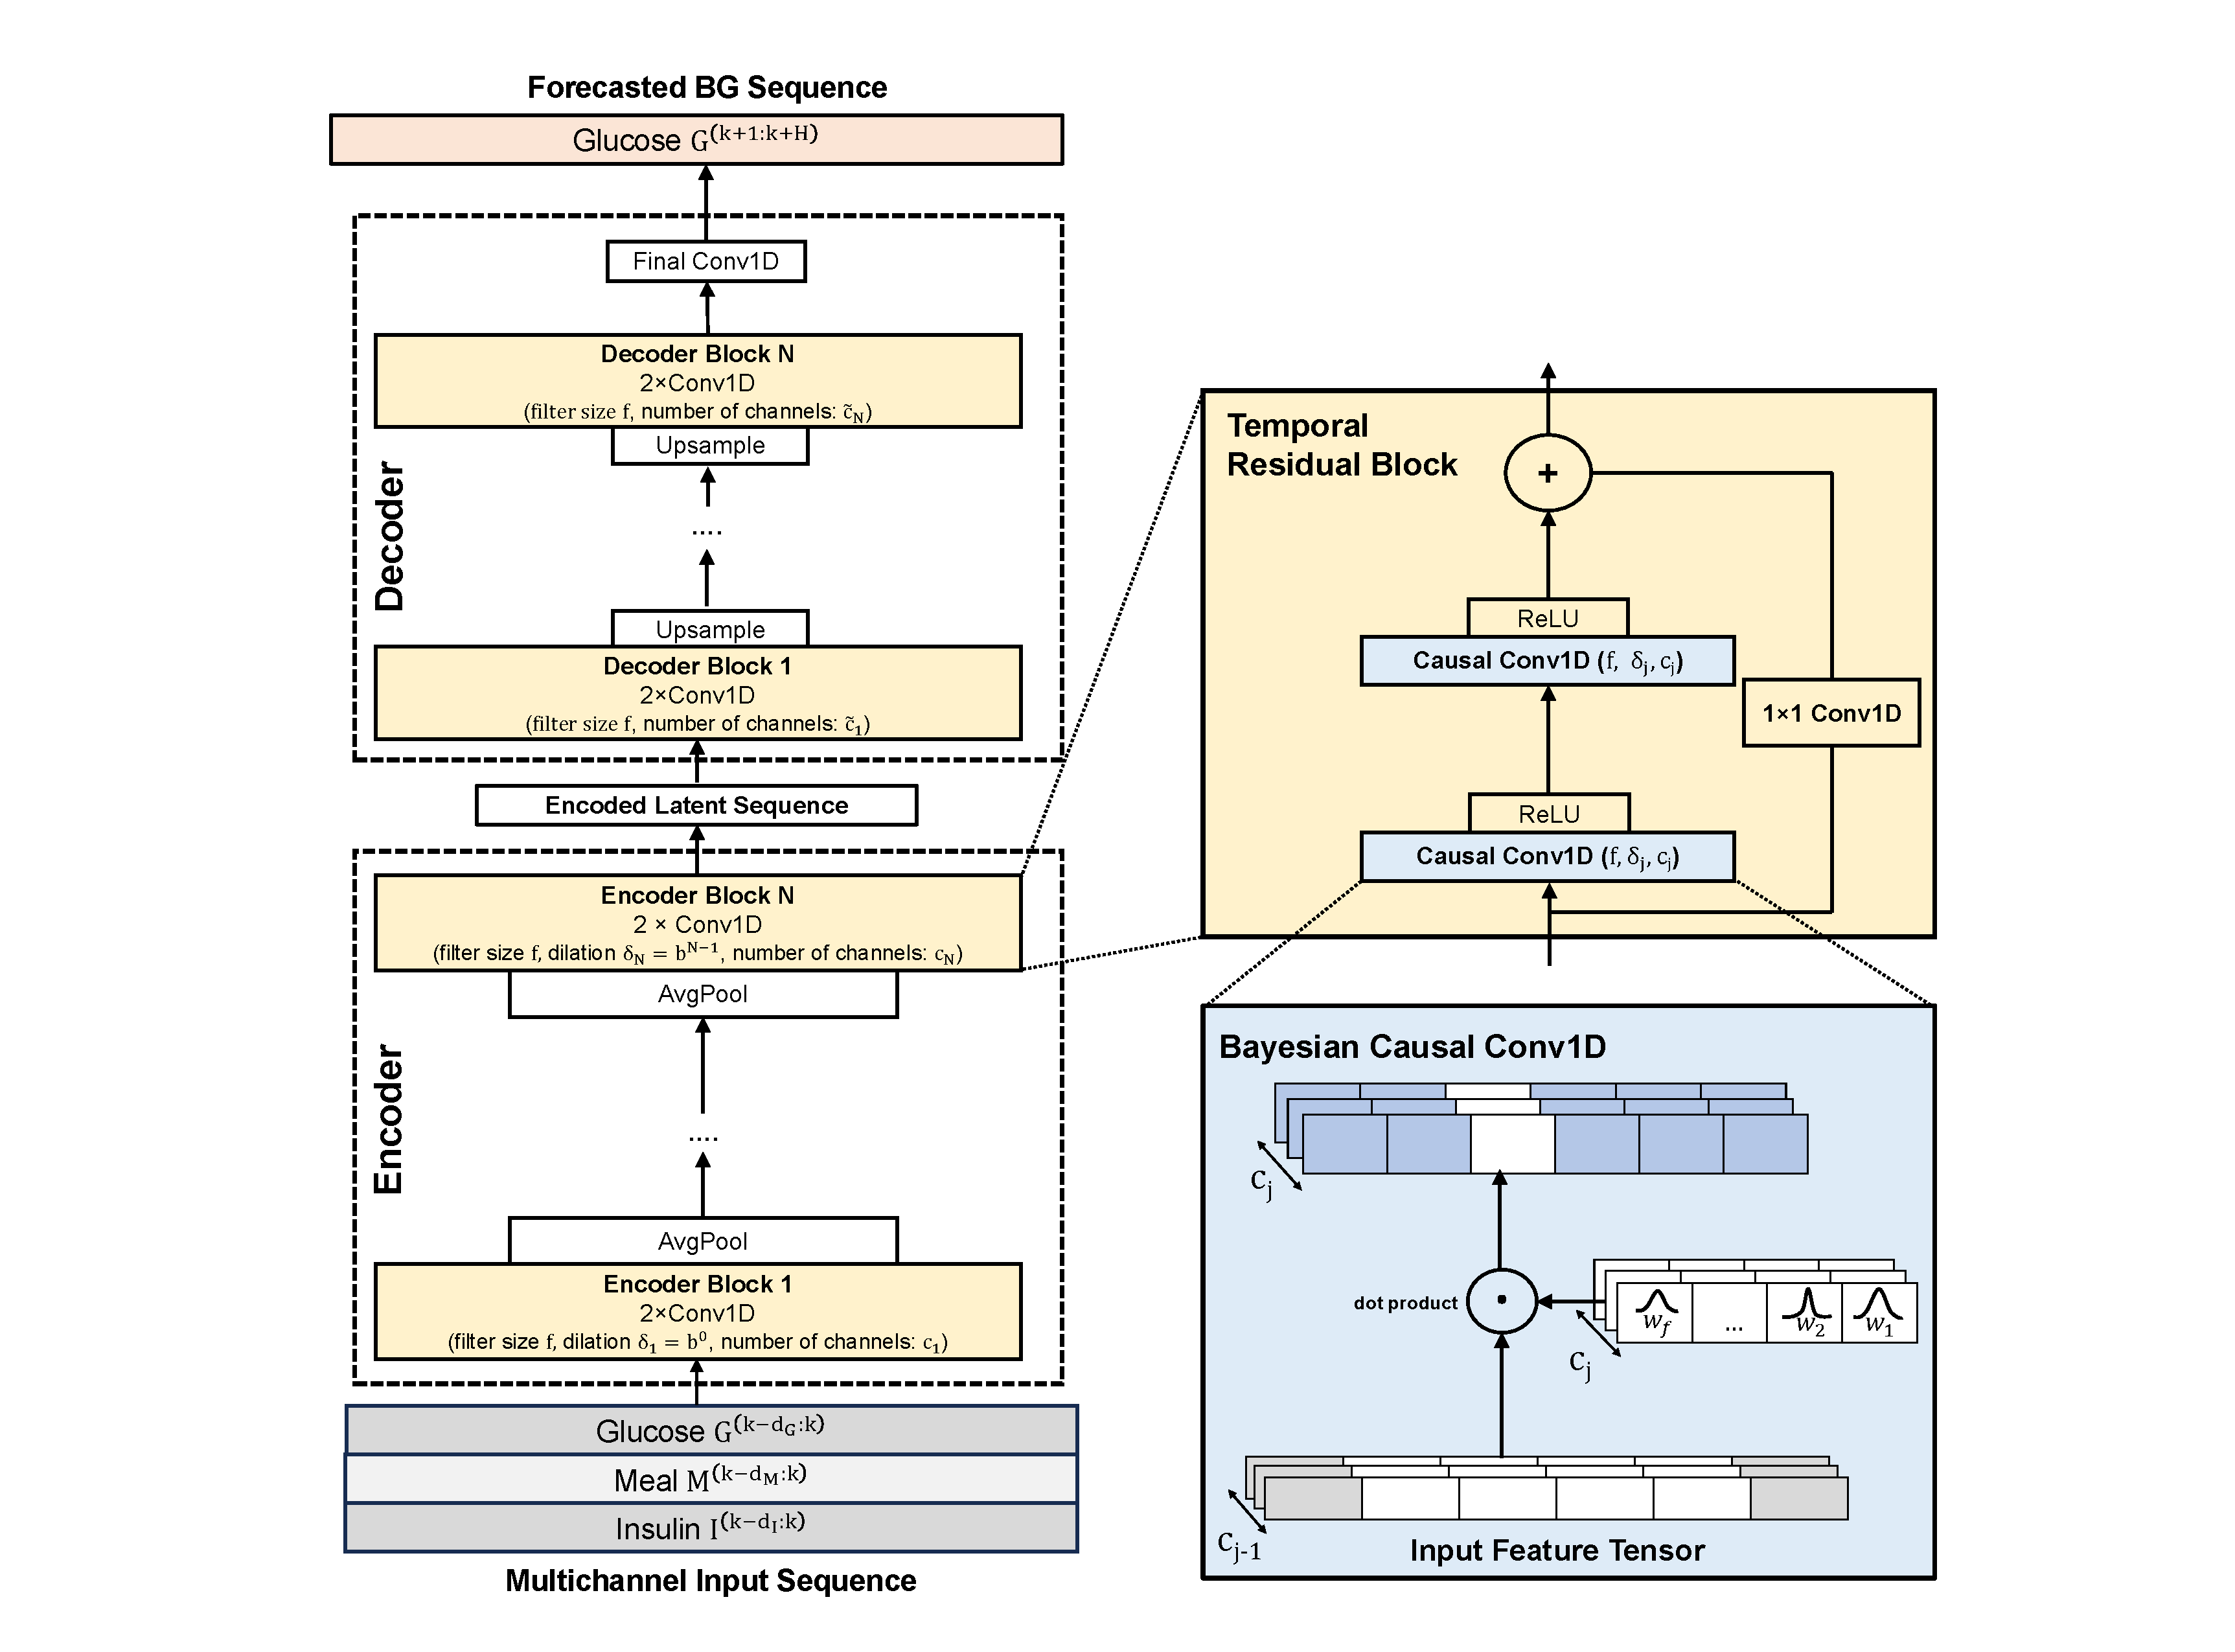
\includegraphics[trim={2.in 0in 2.in 0in}, clip, width=1\linewidth]{Figures_manuscript/full_archi.pdf}
    \vspace{-0.4in}
\caption{
(Left Panel) Bayesian temporal convolutional network (TCN) architecture used for multi-step blood-glucose (BG) forecasting 
${G}^{(k+1:k+H)} = \mathcal{T}_{w,\xi}\!(G^{(k-d_G:k)},\, M^{(k-d_M:k)},\, I^{(k-d_I:k)})$. 
The encoder contains $N$ temporal residual blocks with $c_j$ channels, filter size $f$, and dilation $\delta_j=b^{j-1}$; average-pooling layers between successive encoder blocks progressively reduce the temporal resolution and produce an encoded latent sequence. The decoder consists of $N$ residual convolutional blocks with $\tilde{c}_j$ channels, unit-dilation causal convolutions, and upsampling layers between successive decoder blocks. 
(Top-right Panel) Temporal residual block consisting of two Bayesian causal Conv1D layers with ReLU activations and a residual skip connection; a $1\times1$ Conv1D is used on the skip path when the input and output channel dimensions differ. 
(Bottom-right Panel) The Bayesian parameterization of a causal Conv1D layer, where the convolutional weights are represented by probability distribution determined by Bayesian training.
}
    \label{fig:arch}
\end{figure}

%

Within this architecture family, the receptive field is a derived quantity determined by \(\xi\), indicating set of entries of the input that affect a specific entry of the output. For the temporal blocks in Figure~\ref{fig:arch}, each of which contains two causal dilated convolutions, the resulting receptive field is
\begin{equation}
\mathrm{RF}
=
1+2(f-1)\sum_{j=0}^{N-1} b^j
=
1+2(f-1)\frac{b^N-1}{b-1}.
\label{eq:rf_closed}
\end{equation}
%
The feasible architecture space is defined by the finite combinations of discrete architecture parameters (number of blocks $N$, dilation base $b$, filter size $f$, number of channels in encoder $\{c_j\}_{j=1}^N$ and decoder $\{\tilde{c}_j\}_{j=1}^N$, stride $s$, input lengths $\{d_G, d_M, d_I\}$, and output horizon $H$), subject to structural and temporal constraints,
%
\begin{equation}
\Xi
=
\left\{
\xi :
\mathrm{RF}\geq \tau_{\min},
\;
f \geq b
\right\},
\label{eq:feasible_space}
\end{equation}
where \(\tau_{\min}\) denotes the minimum temporal extent required to capture relevant glucose dynamics (e.g., delayed effects of meals and insulin), and \(f \geq b\) enforces a no-holes condition for dilated convolutions such that every input in the sequence contributes to the output. Additional problem-specific constraints may be imposed based on the desired prediction horizon and computational budget. Despite these restrictions, the combinatorial structure of \(\xi\) induces a large candidate architecture space, motivating the need for a principled architecture discovery strategy.

%++++++++++++++++++++++++++++++++++++++++++++++++++++++++++++++++++++++++
\subsection{Bayesian learning of TCN predictors}\label{sec:tcn_bayes}
We pose the training of the TCN predictor in a Bayesian setting by placing a probability distribution over the trainable parameters, i.e., convolutional weights \(w\). The Bayesian training is motivated by the limited and heterogeneous nature of the data, the need for quantifying uncertainty in the forecasts, and the requirement that architecture selection be robust to overconfident data fits.
%
In our particular problem, training is performed using population-level data obtained from multichannel time series across multiple type 1 diabetes patients. The TCN is trained using a sliding-window procedure with stride \(s\), applied over the full dataset. 
The retrospective data associated with patient $i$ is written as
%
\begin{equation}
\mathcal{D}_i
=
\left\{
\left(
G_{\mathrm{data}, i}^{(k-d_G:k)},\,
M_{\mathrm{data}, i}^{(k-d_M:k)},\,
I_{\mathrm{data}, i}^{(k-d_I:k)},\,
G_{\mathrm{data}, i}^{(k+1:k+H)}
\right)
\right\}_{k=1}^{N_{D_i}}.
\end{equation}
%
Here, \(G_{\mathrm{data}, i}\) denotes the observed glucose trajectory from continuous glucose monitoring (CGM), \(M_{\mathrm{data}, i}\) denotes the recorded meal-related input, and \(I_{\mathrm{data}, i}\) denotes the recorded insulin delivery.
Each index \(k\) corresponds to a sliding temporal window extracted from the trajectory of patient \(i\), and \(N_{D_i}\) denotes the total number of admissible input-output windows obtained from that patient.
%
The complete population-based training dataset constructed from \(N_{\mathrm{patient}}\) patients is then given by
%
\begin{equation}
\mathcal{D}
=
\bigcup_{i=1}^{N_{\mathrm{patient}}}
\mathcal{D}_i .
\end{equation}
%
For a given architecture \(\xi\), Bayesian training is defined by a prior distribution on the weights and a likelihood function for the observed trajectories. We use a Gaussian prior
$
\pi_{\mathrm{pr}}(w | \sigma_{\mathrm{pr}},\xi)
=
\mathcal{N}\!\left(0,\sigma_{\mathrm{pr}}^2 I_{W}\right),
$
%
and assume additive Gaussian noise model with variance \(\sigma_{\mathrm{noise}}^2\), leading to log-likelihood being proportional to
%
\begin{equation}
\log \pi_{\mathrm{like}}(\mathcal{D} \mid w,\sigma_{\mathrm{noise}},\xi)
\;\propto\;
-\frac{1}{2\sigma_{\mathrm{noise}}^2}
\sum_{k=1}^{N_D}
\left\|
G_{\mathrm{data}}^{(k+1:k+H)}
-
\mathcal{T}_{w,\xi}\!\big(G^{(k-d_G:k)}, M^{(k-d_M:k)}, I^{(k-d_I:k)}\big)
\right\|_2^2,
\end{equation}
%
where \(\sigma=(\sigma_{\mathrm{pr}},\sigma_{\mathrm{noise}})\) is called inference hyperparameters and 
\(N_D\) denotes the number of training input--output windows
over all patients.
Under these assumptions, the posterior distribution over the  trainable parameters is given by
\begin{equation}
\label{eq:bayes_w}
\pi_{\mathrm{post}}(w\mid \mathcal{D},\sigma,\xi)
=
\frac{\pi_{\mathrm{like}}(\mathcal{D}\mid w,\sigma_{\mathrm{noise}},\xi)\,\pi_{\mathrm{pr}}(w\mid \sigma_{\mathrm{pr}},\xi)}
{\pi_{\mathrm{evid}}(\mathcal{D}\mid \sigma_{\mathrm{pr}},\sigma_{\mathrm{noise}},\xi)}.
\end{equation}
%
Bayesian inference is intractable for TCNs with high-dimensional parameters using sampling methods. We thus employ variational inference with a tractable variational distribution \(q_{\eta}(w)\), parameterized by \(\eta\), chosen here as a mean-field Gaussian. The optimal variational distribution is obtained by minimizing the Kullback--Leibler divergence to the true posterior, equivalently by maximizing the evidence lower bound (ELBO):
%
\begin{equation}
\eta^{\mathrm{opt}}
=
\arg\min_{\eta}
\left[
\mathrm{KL}\!\left(
q_{\eta}(w)\,\|\,\pi_{\mathrm{pr}}(w \mid \sigma_{\mathrm{pr}},\xi)
\right)
-
\mathbb{E}_{q_{\eta}(w)}
\left[
\log \pi_{\mathrm{like}}(\mathcal{D} \mid w,\sigma_{\mathrm{noise}},\xi)
\right]
\right].
\end{equation}
%
This yields an approximate posterior over the TCN weight parameters.
Given the posterior distribution over \(w\) and fixed \(\sigma\) and \(\xi\), the predictive distribution for a new input sequence is
\begin{align}
\pi\!\left(
G^{*(k+1:k+H)}
\,\middle|\,
G^{(k-d_G:k)},\, M^{(k-d_M:k)},\, I^{(k-d_I:k)},\, \mathcal{D},\, \sigma,\, \xi
\right) = 
\nonumber \\
\int
\pi\!\left(
G^{*(k+1:k+H)}
\,\middle|\,
G^{(k-d_G:k)},\, M^{(k-d_M:k)},\, I^{(k-d_I:k)},\, w,\, \sigma,\, \xi
\right)
\pi_{\mathrm{post}}(w\mid \mathcal{D},\sigma,\xi)\,dw,
\label{eq:posterior_predictive}
\end{align}
%
which integrates the TCN predictions over the learned weight posterior. In practice, this distribution is approximated via Monte Carlo sampling from \(q_{\eta^{\mathrm{opt}}}(w)\), yielding predictive mean trajectories and corresponding uncertainty.


%++++++++++++++++++++++++++++++++++++++++++++++++++++++++++++++++++++++++
\subsection{Evidence as an architecture selection criterion}
\label{sec:plausibility}

To move from single-model Bayesian training to architecture discovery, we use the evidence distribution in \eqref{eq:bayes_w} as the scoring function for selecting the inference hyperparameters \(\sigma=(\sigma_{\mathrm{pr}},\sigma_{\mathrm{noise}})\) and for comparing candidate architectures $\xi$. The evidence provides a principled trade-off between data fit and learned parameter uncertainty \cite{mackay1995probable, singh2024framework, immer2021scalable}, and thereby expected to favor models with robust predictive performance based on the available data.
%
For fixed \(\sigma\) and \(\xi\), the evidence is defined as
$
\pi_{\mathrm{evid}}(\mathcal{D} | \sigma,\xi)
=
\int
\pi_{\mathrm{like}}(\mathcal{D} | w,\sigma_{\mathrm{noise}},\xi)\,
\pi_{\mathrm{pr}}(w | \sigma_{\mathrm{pr}},\xi)\,dw.
$
This quantity evaluates how well the architecture \(\xi\), together with \(\sigma\), explains the training data after marginalizing over parameter uncertainty. The posterior over the inference hyperparameters is given by
\begin{equation}
\pi_{\mathrm{post}}(\sigma\mid \mathcal{D},\xi)
=
\frac{
\pi_{\mathrm{evid}}(\mathcal{D}\mid \sigma,\xi)\,
\pi_{\mathrm{pr}}(\sigma\mid \xi)
}{
\pi_{\mathrm{evid}}(\mathcal{D}\mid \xi)
}.
\label{eq:sigma_post}
\end{equation}
%
In this work, \eqref{eq:sigma_post} is approximated using a Laplace approximation, yielding a maximum a posteriori estimate of \(\sigma_{\mathrm{MAP}}\). Details of this approximation are provided in ~\ref{app:evidence} and follow \cite{singh2024framework}.
%
Given \(\sigma_{\mathrm{MAP}}\), the architecture-level evidence is obtained by marginalizing over \(\sigma\),
$
\pi_{\mathrm{evid}}(\mathcal{D}| \xi)
=
\int
\pi_{\mathrm{evid}}(\mathcal{D} | \sigma,\xi)\,
\pi_{\mathrm{pr}}(\sigma | \xi)\,d\sigma,
$
which is again approximated via Laplace Approximation (see~\ref{app:evidence}).
%
Let \(\mathcal{M}=\{\xi_m\}_{m=1}^{M}\) denote the finite candidate architecture set. The posterior plausibility of architecture \(\xi_m\) is defined as
\begin{equation}
\rho_m
=
\pi_{\mathrm{post}}(\xi_m\mid \mathcal{D})
=
\frac{
\pi_{\mathrm{evid}}(\mathcal{D}\mid \xi_m)\,
\pi_{\mathrm{pr}}(\xi_m)
}{
\sum_{j=1}^{M}
\pi_{\mathrm{evid}}(\mathcal{D}\mid \xi_j)\,
\pi_{\mathrm{pr}}(\xi_j)
},
\qquad m=1,\ldots,M.
\label{eq:rho_m}
\end{equation}
Under a uniform prior over architectures, \(\rho_m\) reduces to normalized evidence.
%
The plausibility weights \(\{\rho_m\}_{m=1}^{M}\) can be used either to select the most plausible architecture $\xi_{\mathrm{plausible}}=\arg\max_{\xi \in \Xi} \rho$ or to form a plausibility-weighted ensemble predictor:
\begin{eqnarray}
\pi\!\left(
G^{* (k+1:k+H)}
\,\middle|\,
G^{(k-d:k)},\,M^{(k-d:k)},\,I^{(k-d:k)},\,\mathcal{D}
\right) =
\nonumber \\
\sum_{m=1}^{M}
\rho_m\,
\pi\!\left(
G^{* (k+1:k+H)}
\,\middle|\,
G^{(k-d:k)},\,M^{(k-d:k)},\,I^{(k-d:k)},\,\mathcal{D},\,\xi_m
\right).
\label{eq:bma}
\end{eqnarray}


%++++++++++++++++++++++++++++++++++++++++++++++++++++++++++++++++++++++++
\subsection{EVIDENT: Evidence-based identification
of neural architectures}\label{sec:evident}
EVIDENT is a iterative architecture discovery strategy that combines Bayesian training, evidence-based ranking, and validation under uncertainty to identify TCN predictors with accurate and reliable task-specific performance. Rather than exhaustively searching a potentially large candidate pool, EVIDENT proceeds level by level, determining high-plausibility regions of the architecture space and testing whether the resulting models satisfy the prescribed validation criteria. In this way, the framework balances predictive performance and model complexity while avoiding unnecessary exploration of architectures that are either insufficiently expressive or overly parameterized. An algorithmic summary of EVIDENT is provided in Figure~\ref{fig:algorithm} and various components are described here.

%

\paragraph{Candidate pool and capacity levels}
Let \(\mathcal{M}_{\mathrm{initial}}=\{\xi_m\}_{m=1}^{M}\) denote the finite, but potentially large, candidate architecture set induced by the feasible architecture space. EVIDENT partitions this set into ordered capacity levels,
$
\mathcal{M}_{\mathrm{initial}}
=
\bigcup_{l=1}^{L}\mathcal{M}^{(l)},
\;
\mathcal{M}^{(l)}\cap \mathcal{M}^{(r)}=\varnothing
\ \text{for}\ l\neq r,
$
where the levels are arranged from lower to higher model capacity according to a prescribed complexity measure, such as the number of trainable parameters. This construction avoids committing apriori to either overly small architectures, which may lack sufficient expressive power, or highly over-parameterized architectures, whose parameters cannot be reliably informed by the available data. Instead, EVIDENT searches progressively over increasingly expressive architecture classes guided by posterior plausibility.

%

\paragraph{Level-wise architecture ranking}
For each level \(l\), every candidate architecture \(\xi \in \mathcal{M}^{(l)}\) is trained using the Bayesian learning procedure in \eqref{eq:bayes_w}. The corresponding posterior plausibility values \(\rho(\xi)\) are then computed from \eqref{eq:rho_m}, and the architectures are ranked accordingly. 
Let \(\widehat{\mathcal{M}}^{(l)} \subseteq \mathcal{M}^{(l)}\) denote the resulting shortlist of top-ranked architectures. In the simplest case, \(\widehat{\mathcal{M}}^{(l)}\) contains only the most plausible architecture in level \(l\); more generally, it may include several architectures with comparable evidence. Only the architectures in \(\widehat{\mathcal{M}}^{(l)}\) are then advanced to the validation process.

%

%---------------
\begin{figure}[t]
\centering
\fbox{
\begin{minipage}{0.92\linewidth}
\textbf{EVIDENT: EVidence-based IDEntification of Neural archiTectures}

\vspace{0.3em}
\textbf{Input:} Initial architecture pool \(\mathcal{M}_{\mathrm{initial}}=\{\xi_m\}_{m=1}^M\), 
training data \(\mathcal{D}\), 
validation data \(\mathcal{D}_{\mathrm{val}}\), 
tolerance \(Tol\).

\textbf{Output:} Architectures identified as trustworthy predictors.

\vspace{0.3em}
\textbf{Procedure:}
\begin{enumerate}
\item Partition \(\mathcal{M}_{\mathrm{initial}}\) into levels \(\{\mathcal{M}^{(l)}\}_{l=1}^L\).
\item For \(l=1,\dots,L\):
\begin{enumerate}
\item Train \(\xi \in \mathcal{M}^{(l)}\) on \(\mathcal{D}\) via Bayesian inference.
\item Rank by plausibility \(\rho(\xi)\) and retain top-ranked in \(\widehat{\mathcal{M}}^{(l)} \subseteq \mathcal{M}^{(l)}\).
\item Validate \(\xi \in \widehat{\mathcal{M}}^{(l)}\) on \(\mathcal{D}_{\mathrm{val}}\):
\[
\mathbb{d}\!\left(\mathcal{D}_{\mathrm{val}},\,\mathcal{T}_{\xi}\right)\leq Tol.
\]
\item Return accepted architecture(s) as trustworthy predictor(s) and terminate.
\end{enumerate}
\item If none accepted, expand \(\mathcal{M}_{\mathrm{initial}}\) and repeat.
\end{enumerate}
\end{minipage}
}
\caption{EVIDENT workflow. Architectures are explored from lower to higher capacity, ranked by evidence, and validated using a task-specific probabilistic metric \(\mathbb{d}\) (e.g., NLPD). The procedure returns the simplest architecture(s) satisfying the validation criterion, yielding trustworthy predictors.}
\label{fig:algorithm}
\end{figure}
%---------------

\paragraph{Task-specific validation under uncertainty}
This stage is the central step in EVIDENT as it is not intended to measure prediction accuracy on arbitrary held-out dataset; rather, it tests whether an architecture delivers sufficiently accurate and reliable predictions for the intended deployment regime. Accordingly, the validation design must be problem-specific and aligned with the target use case. In the diabetes application considered in the next section, validation is designed to identify TCN architectures that generalize from population-level training data to unseen individual patients and remain trustworthy for insulin-control decisions. Validation is performed across holdout folds. In each fold, the posterior predictive distribution of competitive architectures, is compared against the observed trajectories of the held-out individual patients.
%
Acceptance is determined using one or more probabilistic validation criteria together with a prescribed tolerance $Tol$.
In this work, the primary validation metric is the negative log predictive density (NLPD),
%
\begin{equation} 
\mathrm{NLPD} = \frac{1}{N_{\mathrm{val}}} \sum_{i=1}^{N_{\mathrm{val}}} \left[ \frac{ \left\| G_{\mathrm{data},i}^{(k+1:k+H)} - \overline{\mathcal{T}}_{w,\xi}\!\left( G_{\mathrm{data},i}^{(k-d_G:k)}, M_{\mathrm{data},i}^{(k-d_M:k)}, I_{\mathrm{data},i}^{(k-d_I:k)} \right) \right\|_2^2 }{2\sigma_i^2} + \frac{H}{2}\log \sigma_i^2 \right], 
\label{eq:nlpd} 
\end{equation} 
%
where \(N_{\mathrm{val}}\) is the number of validation windows in the holdout fold, \(\overline{\mathcal{T}}_{w,\xi}\) denotes the posterior predictive mean of the TCN forecast, and 
%
\begin{equation} 
\sigma_i^2 = \sigma_{\mathrm{data}}^2 + \mathrm{Var}\!\left[ \mathcal{T}_{w,\xi}\!\left( G_{\mathrm{data},i}^{(k-d_G:k)}, M_{\mathrm{data},i}^{(k-d_M:k)}, I_{\mathrm{data},i}^{(k-d_I:k)} \right) \right]. 
\label{eq:sigma_nlpd} 
\end{equation} 
%
Here, \(\sigma_{\mathrm{data}}^2\) represents the intrinsic uncertainty of the glucose measurements such as CGM sensor noise, while the second term captures predictive variance induced by the Bayesian TCN.
NLPD penalizes both inaccurate forecasts and unreliable predictive, making it a natural criterion for assessing probabilistic forecasting. A candidate architecture is accepted as ``trustworthy predictor'' if it satisfies a prescribed tolerance, i.e., \(\mathrm{NLPD} \leq Tol\), possibly together with additional task-dependent validation requirements.

%

\paragraph{Iterative search and stopping criteria}
If at least one candidate in level \(l\) satisfies the validation criteria, the search terminates and EVIDENT returns the corresponding architecture as trustworthy predictor(s). Otherwise, the algorithm advances to the next level, \(l \leftarrow l+1\), and repeats the training, architecture ranking, and validation under uncertainty cycle. EVIDENT therefore discovers the lowest-capacity architecture that satisfies the fit-for-purpose validation requirements under predictive uncertainty. If no candidate passes validation in the final level, the candidate architecture set must be expanded. The resulting workflow favors plausible architectures supported by the training data and validated for the intended predictive task.






%========================================================
% Results
%========================================================
\section{Results}\label{sec:results}

This section evaluates the Bayesian TCN and the proposed EVIDENT framework through two numerical studies. We first consider a single-patient setting to analyze how evidence varies across the TCN architecture space and whether it identifies architectures that balance expressivity and reliable forecasting. We then apply EVIDENT to population-based type 1 diabetes data from in silico patients to perform architecture discovery under inter-patient variability, with the goal of identifying TCN predictors that generalize reliably to unseen subjects.
%
All Bayesian TCN models were implemented in PyTorch \cite{paszke2019pytorch} and trained using the variational inference code adapted from the open-source repository by  \cite{shridhar2019comprehensive, deighan_2026_20044677}.

%++++++++++++++++++++++++++++++++++++++++++++++++++++++++++++++++++++++++
\subsection{Bayesian plausibility analyses of TCN architectures}
\label{sec:plausibility_results}
We begin with a single-patient forecasting study to examine how Bayesian evidence responds to TCN architecture choices and whether it provides a consistent criterion for navigating the architecture space. This includes the analyses of how evidence varies with architectural complexity and its relationship to accuracy and uncertainty in predicted blood glucose trajectories. This experiment isolates the role of evidence as a selection metric before moving to population-level architecture discovery in the next section.
%
\begin{figure}[!ht]
    \centering
        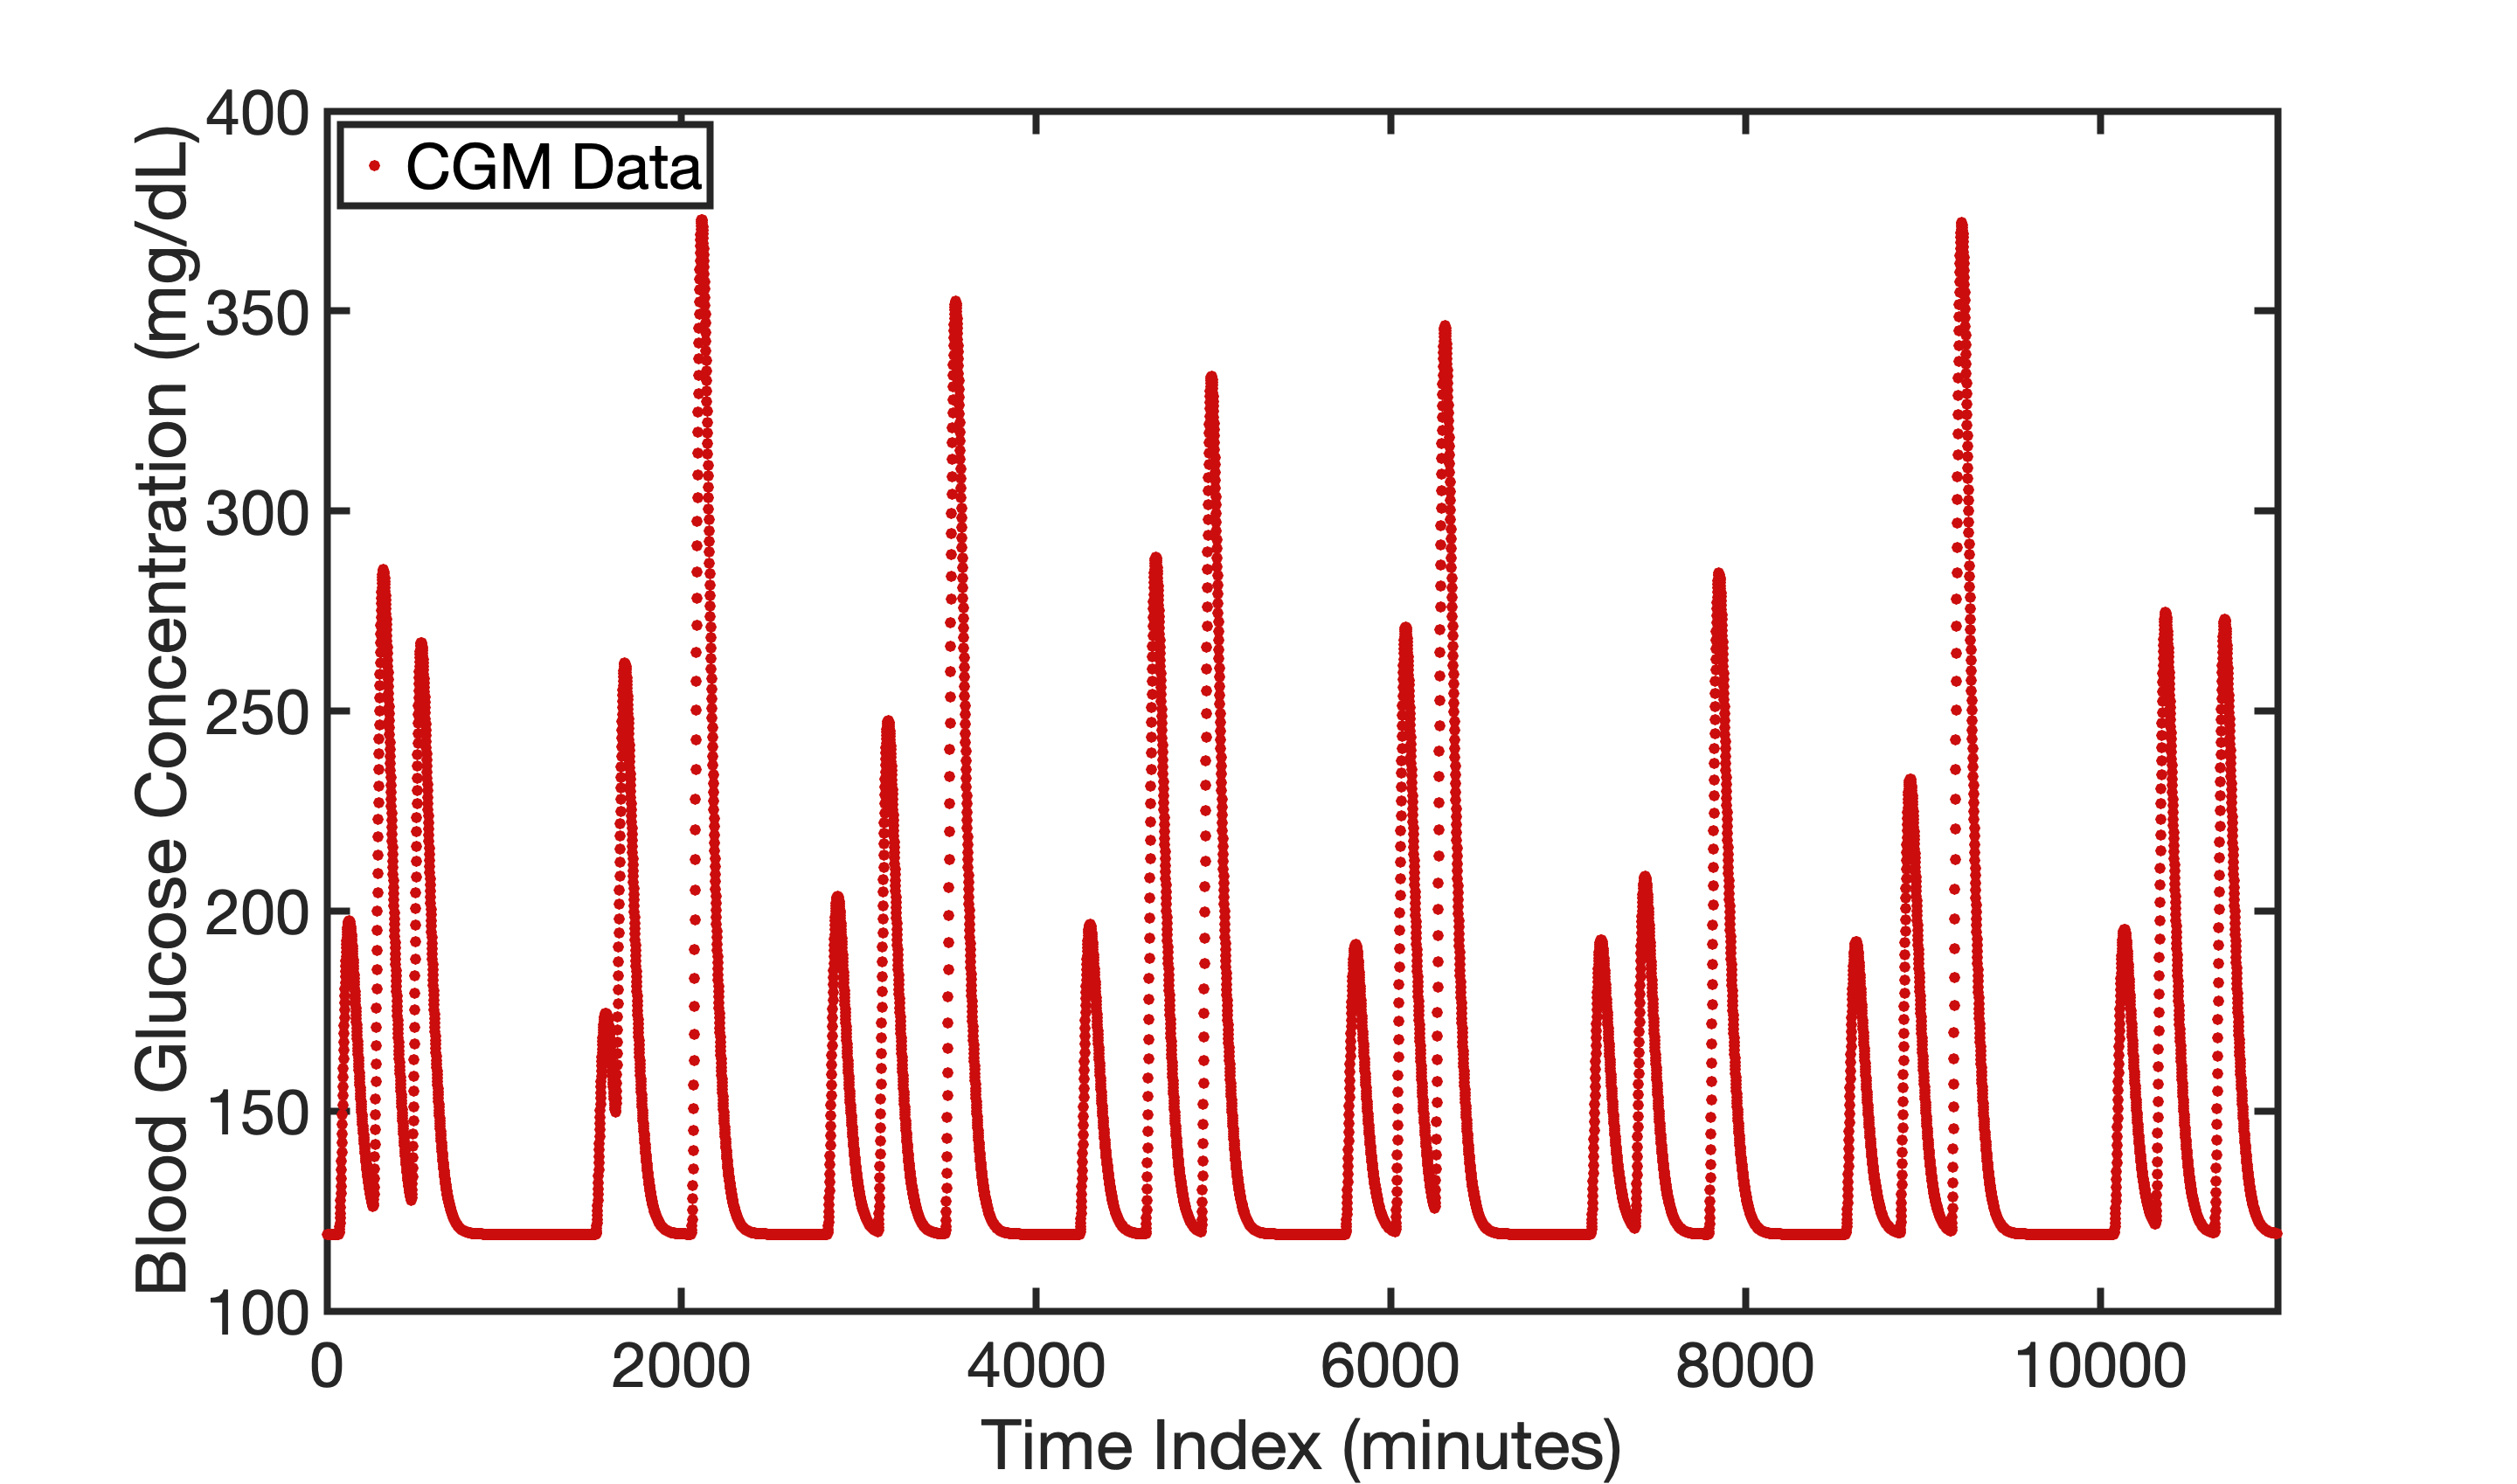
\includegraphics[width=0.5\linewidth]{Figures_manuscript/bergman_data.png}
        \\{\small (a)}\\
        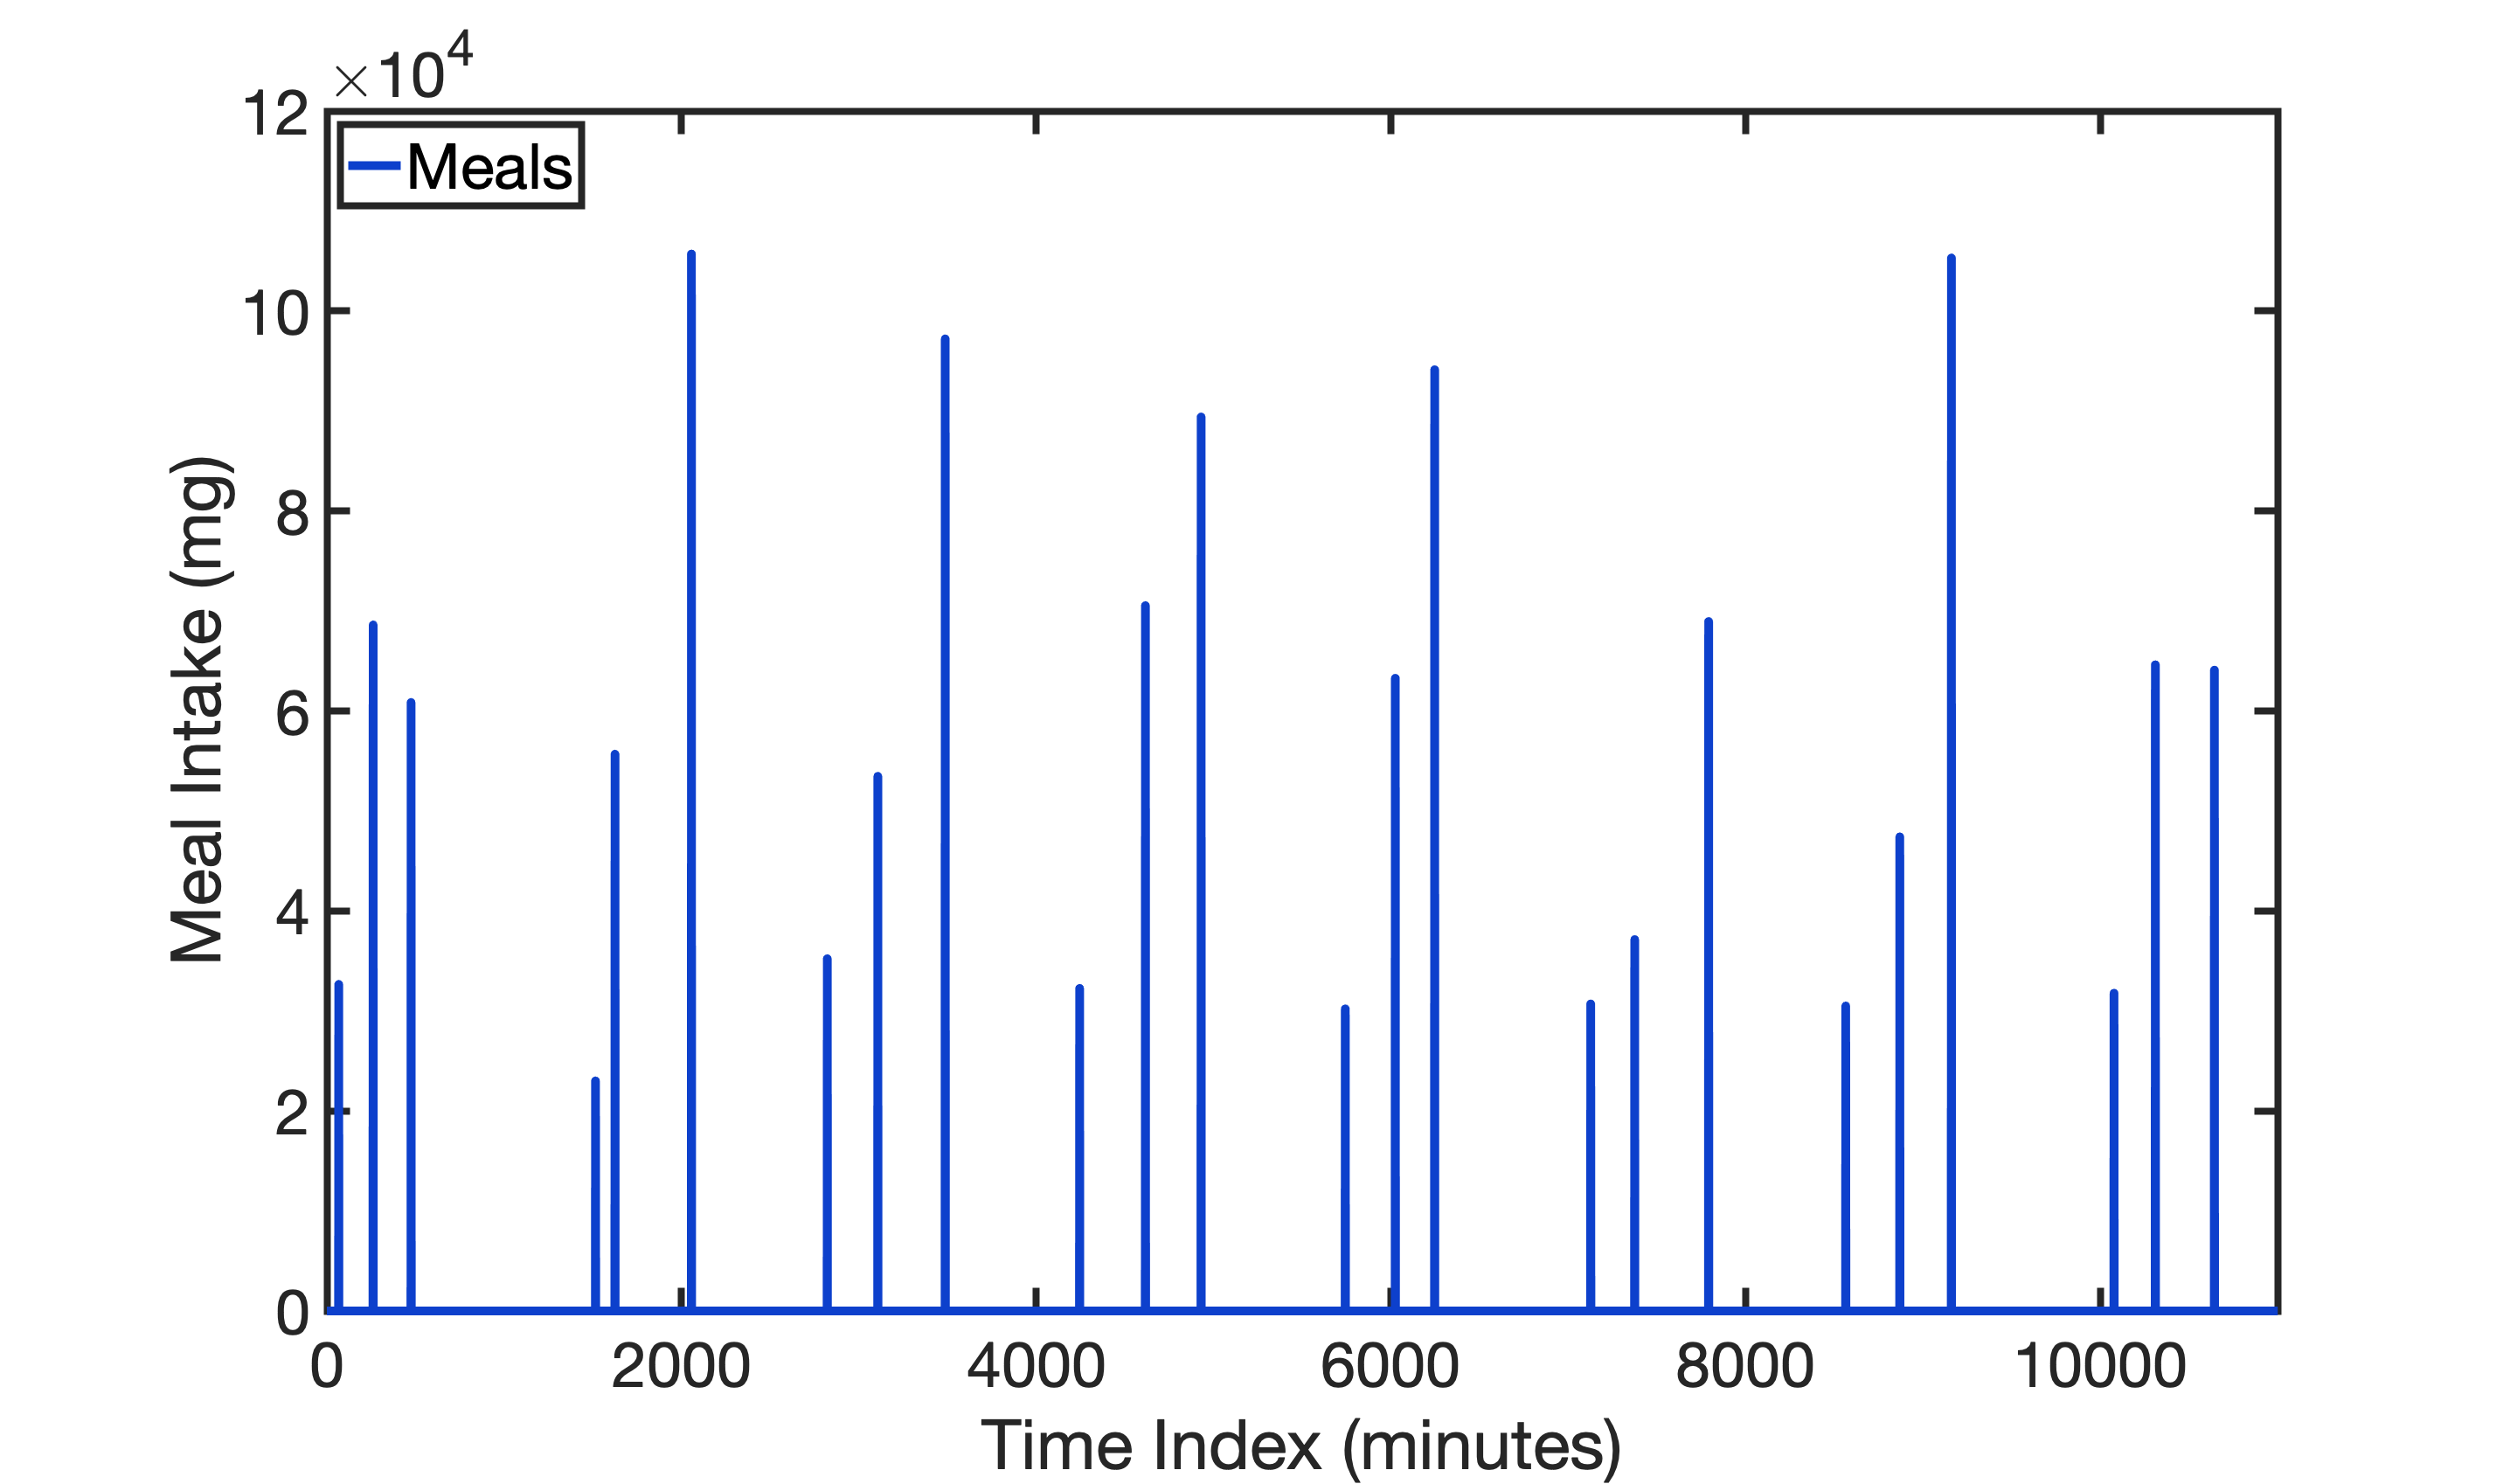
\includegraphics[width=0.4\linewidth]{Figures_manuscript/meal_bergman.png}
        ~
        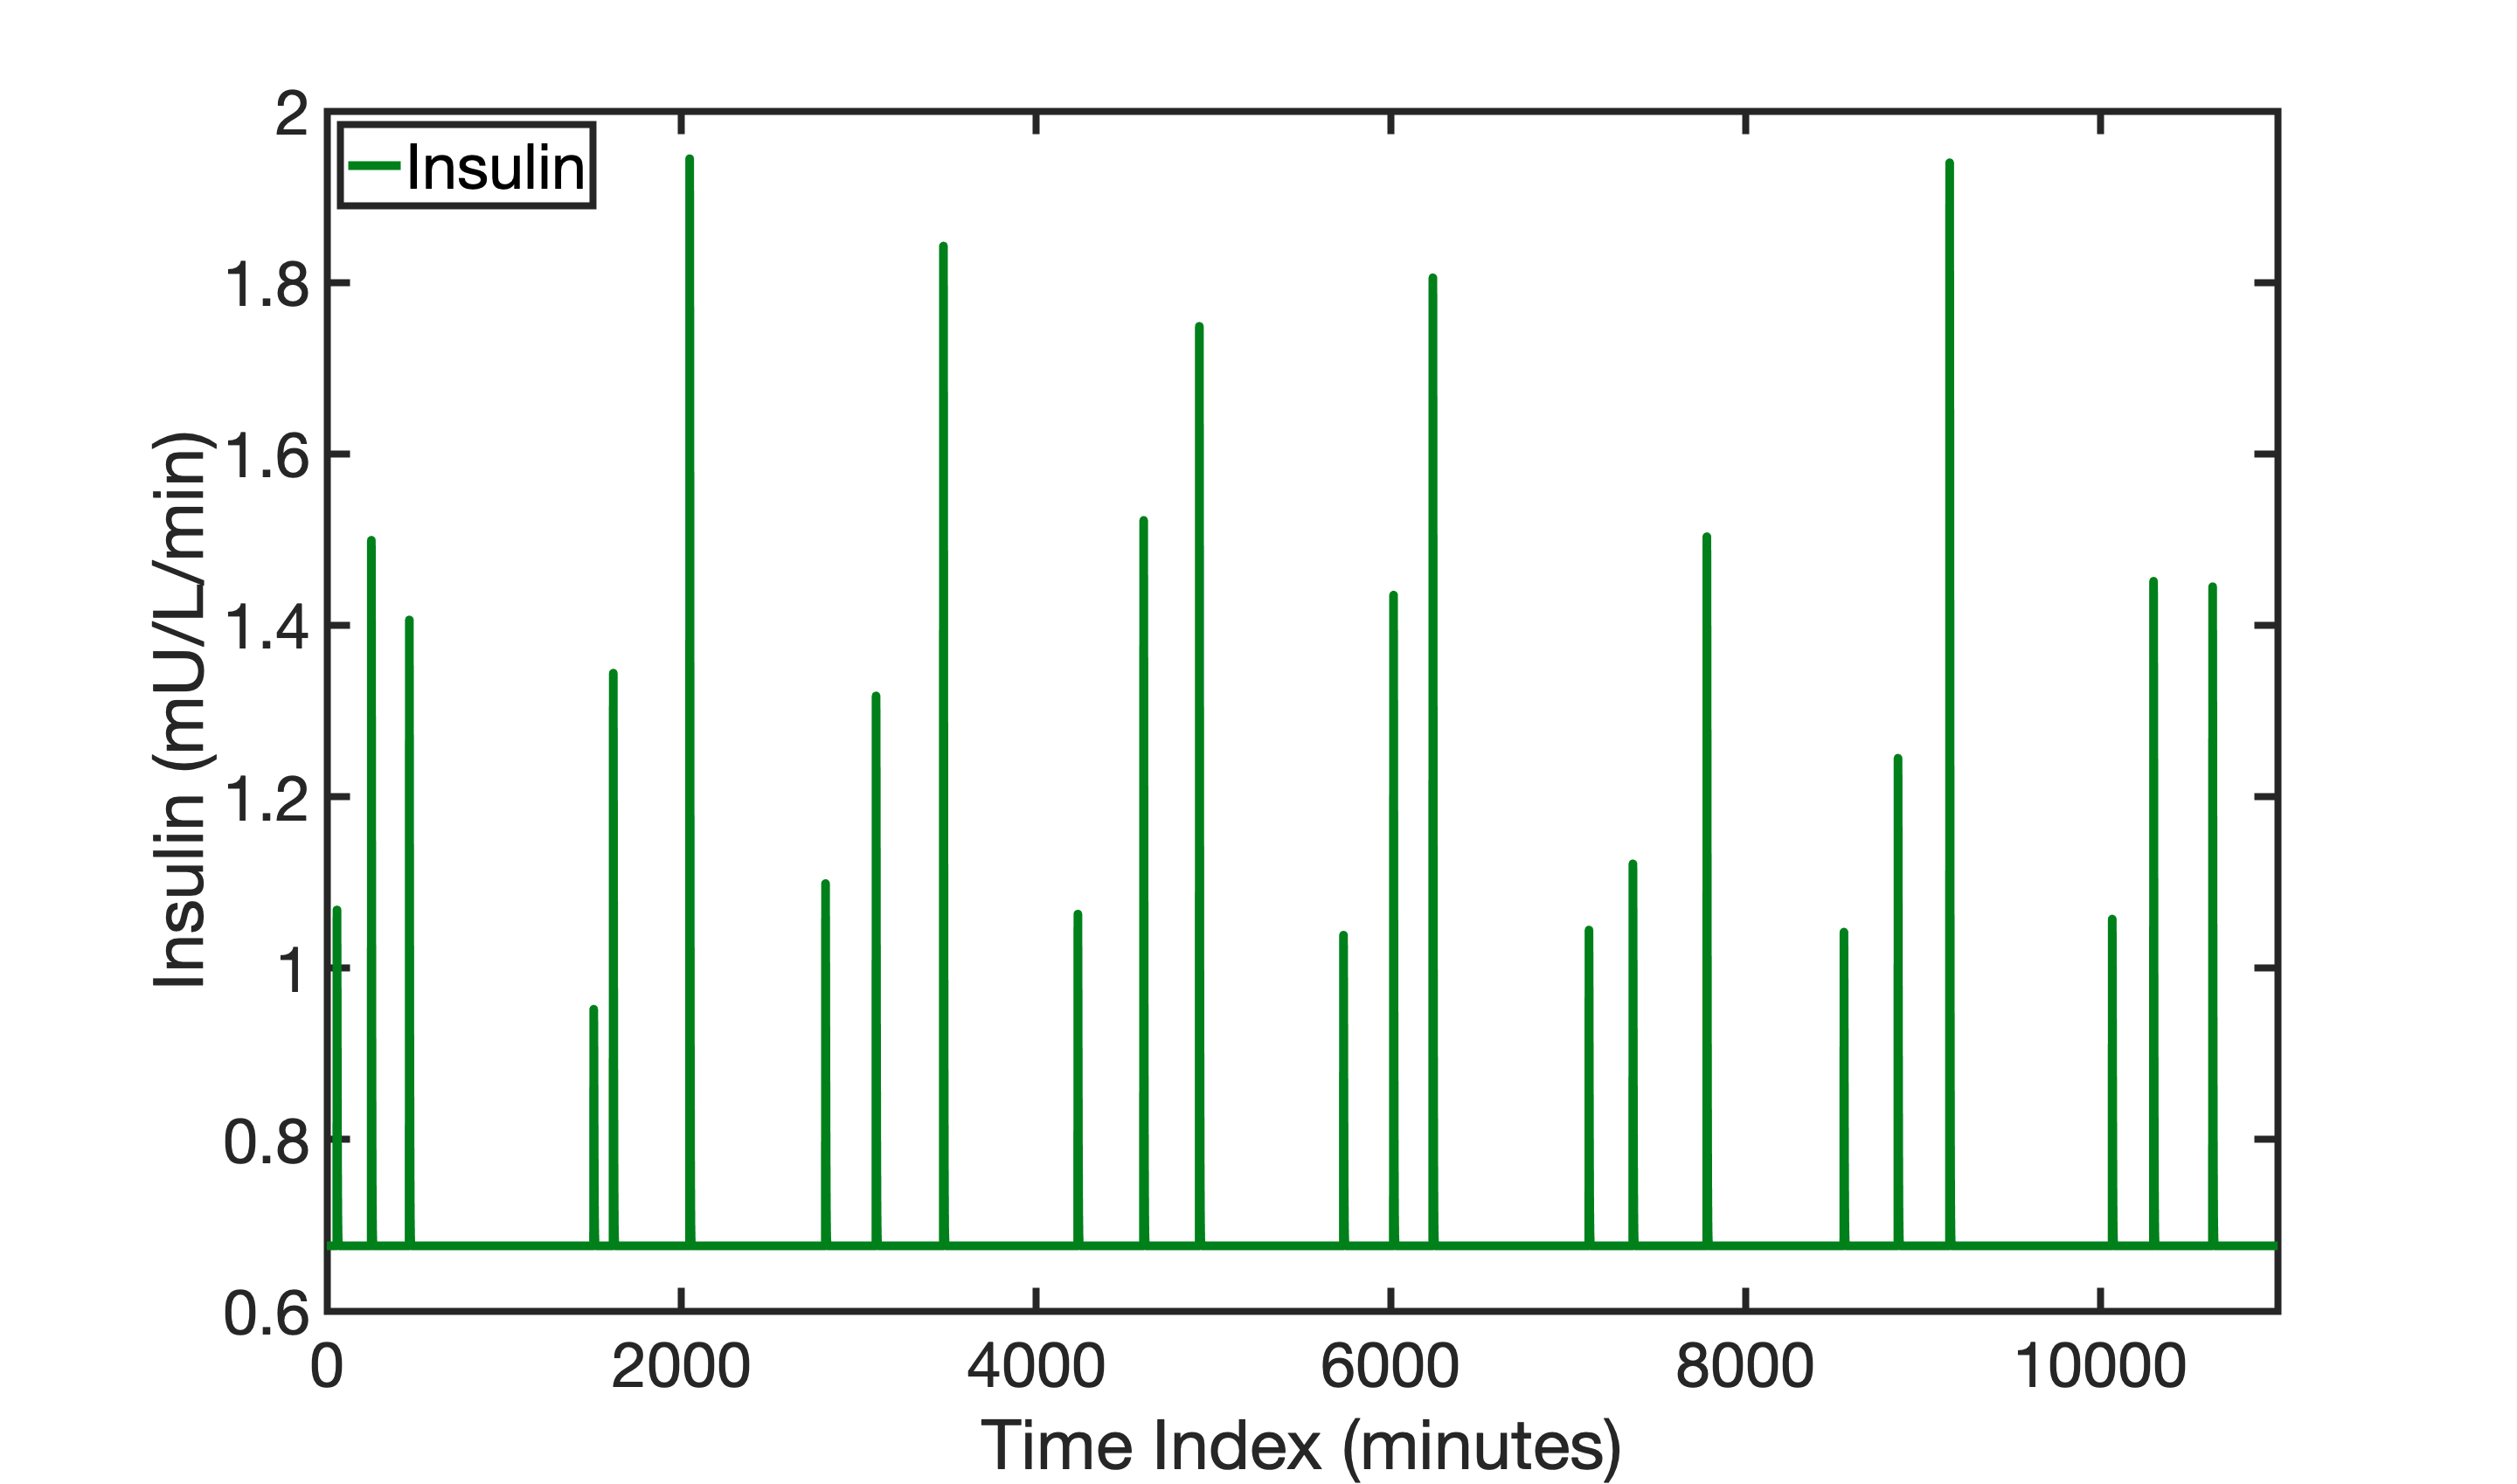
\includegraphics[width=0.4\linewidth]{Figures_manuscript/insulin_bergman.png}
        \\{\small (b) \hspace{2.6in} (c)}\\
    \caption{Single-patient training data used in the plausibility analysis: (a) blood glucose (CGM), (b) meal intake, and (c) insulin delivery, generated using the Bergman minimal model with Dalla Man meal absorption dynamics.}
    \label{fig:bergman}
\end{figure}
%
Figure~\ref{fig:bergman} shows the dataset generated from the Bergman minimal model with meal disturbances modeled via the Dalla Man absorption model \cite{bergman1981physiologic, dalla2006system}. To introduce variability, meal size and timing are randomly perturbed around nominal values, while insulin is administered using a deterministic basal–bolus protocol. Detailed model equations and parameter values are provided in the ~\ref{app:bergman}. 
In all TCNs, the input sequences for glucose $G$, meal $M$, and insulin $I$ share a common history window, i.e., $d_G = d_M = d_I$ in \eqref{eq:tcn_operator}.
All the upcoming results in this section were obtained using the same 90\% train and 10\% test split of the time series shown in Figure~\ref{fig:bergman}. 
%For the dataset underlying Figure~\ref{fig:bergman}, the data spans from \(0\) to \(11520\) minutes. 
The training set corresponds to \(0\text{--}10000\) minutes ($\approx 7$ days) and the test set corresponds to \(10000\text{--}11520\) minutes ($\approx 1$ day).

% -- Evidence vs # blocks/dilation
\begin{figure}[!ht]
\centering
\setlength{\tabcolsep}{4pt}
\renewcommand{\arraystretch}{1.0}

% Top row: architecture descriptors
\begin{tabular}{ccc}
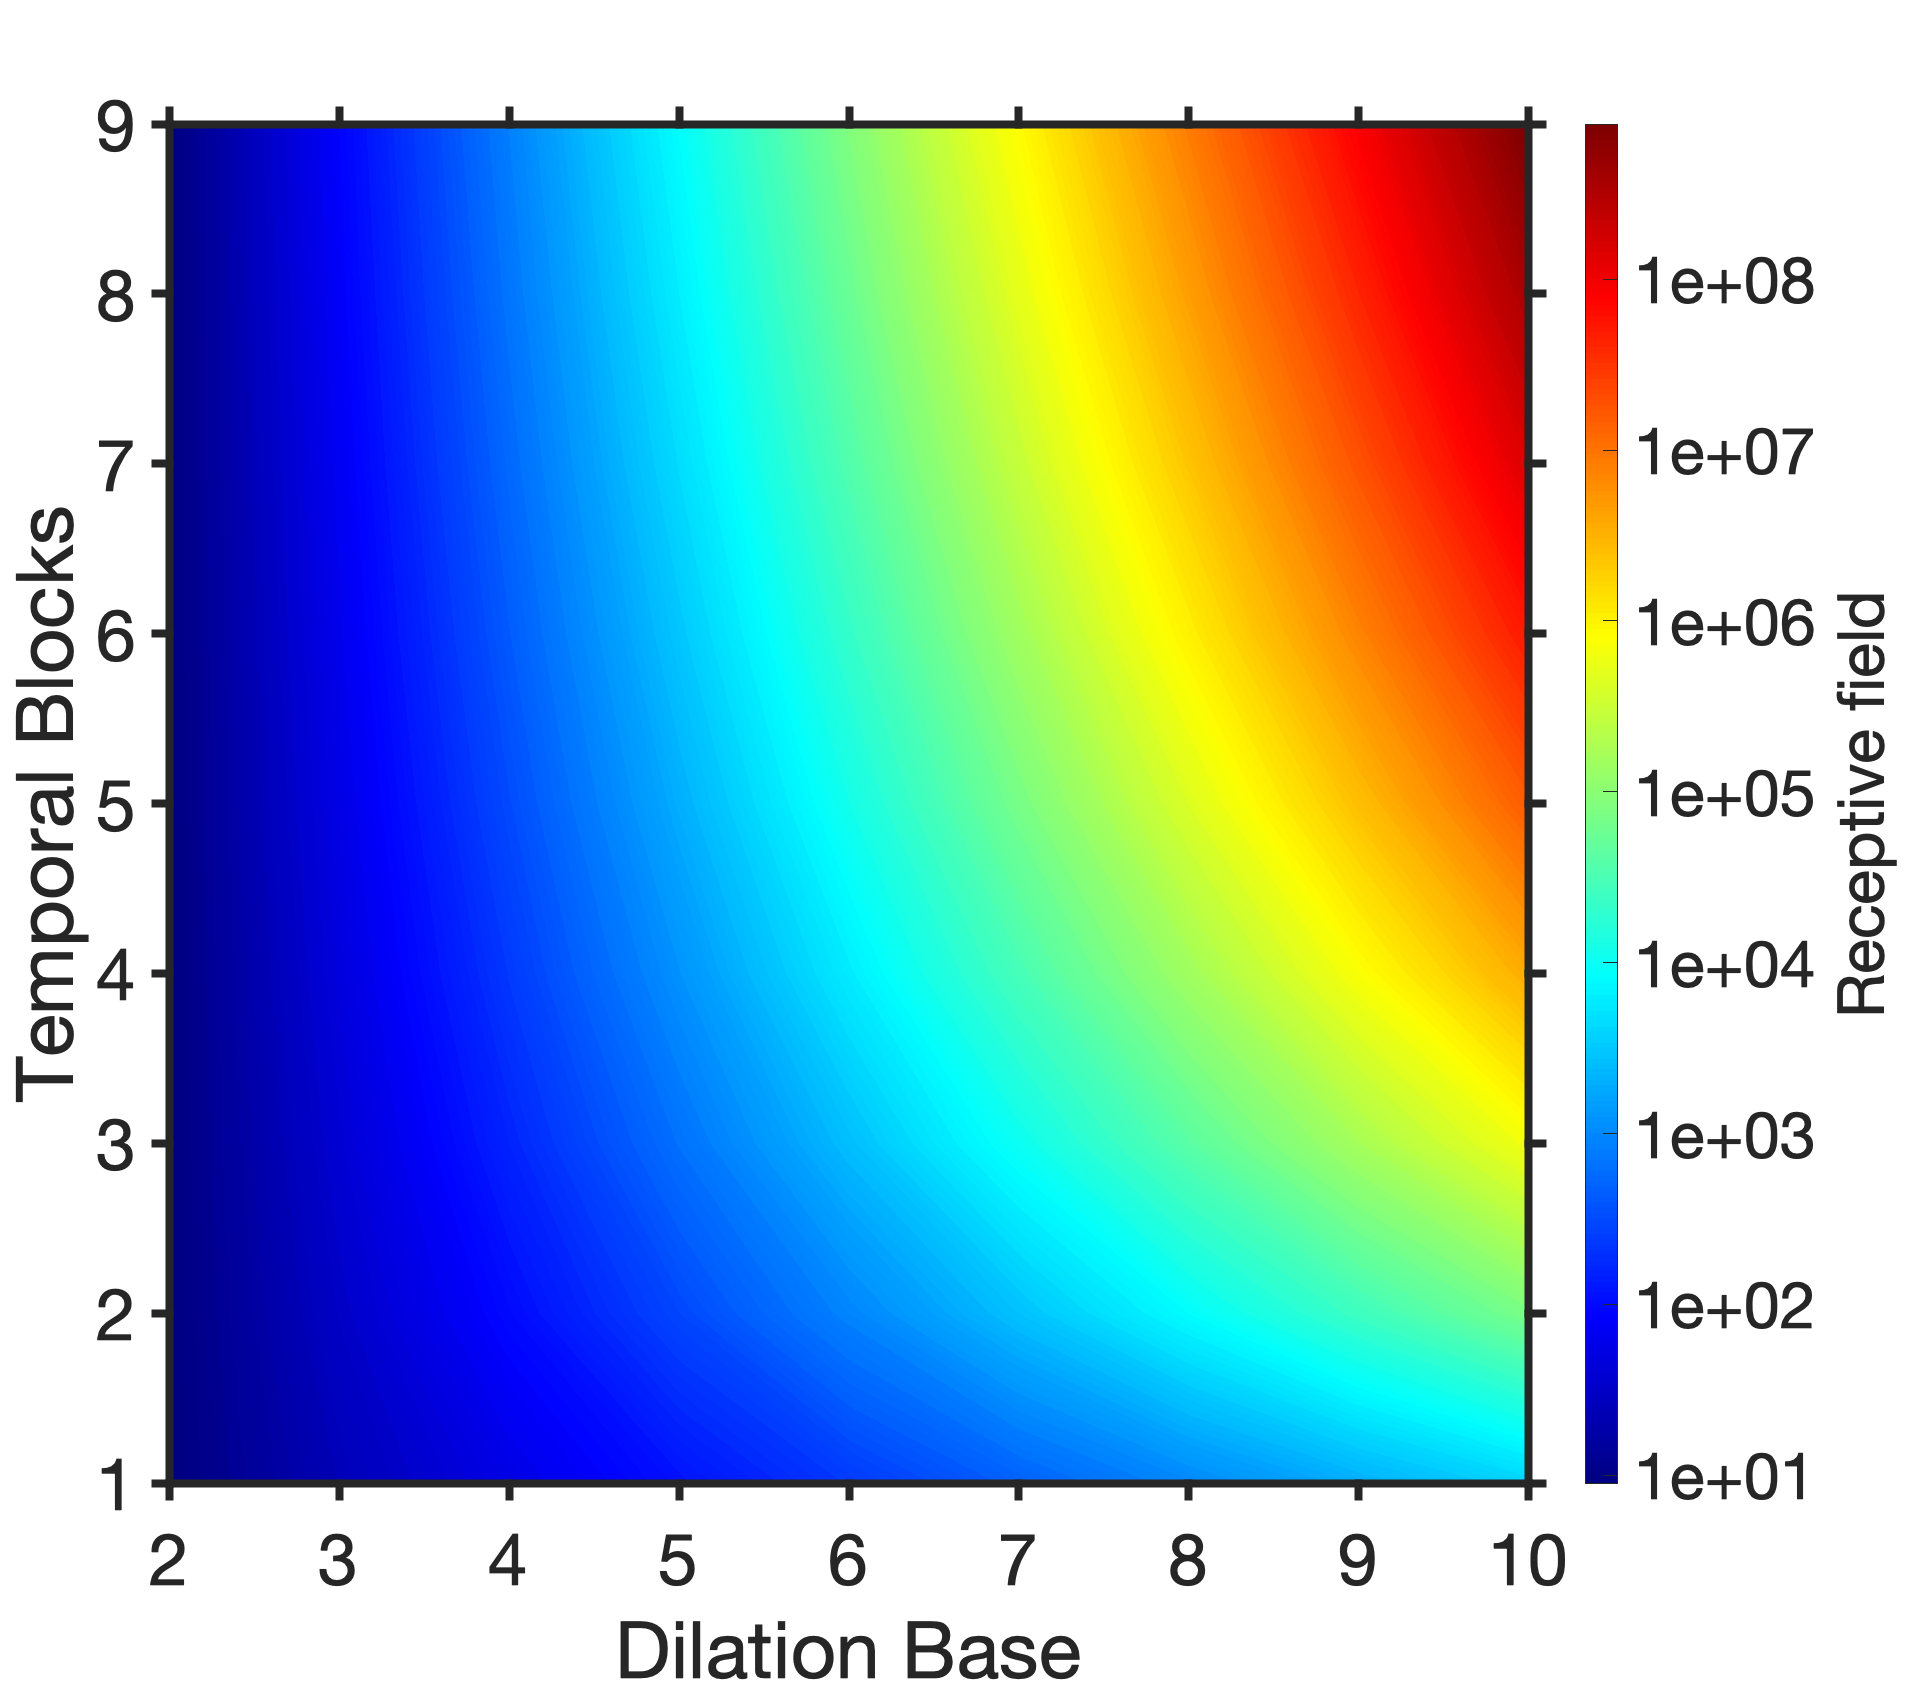
\includegraphics[width=0.28\textwidth]{Figures_manuscript/temp_dil_rf.png} &
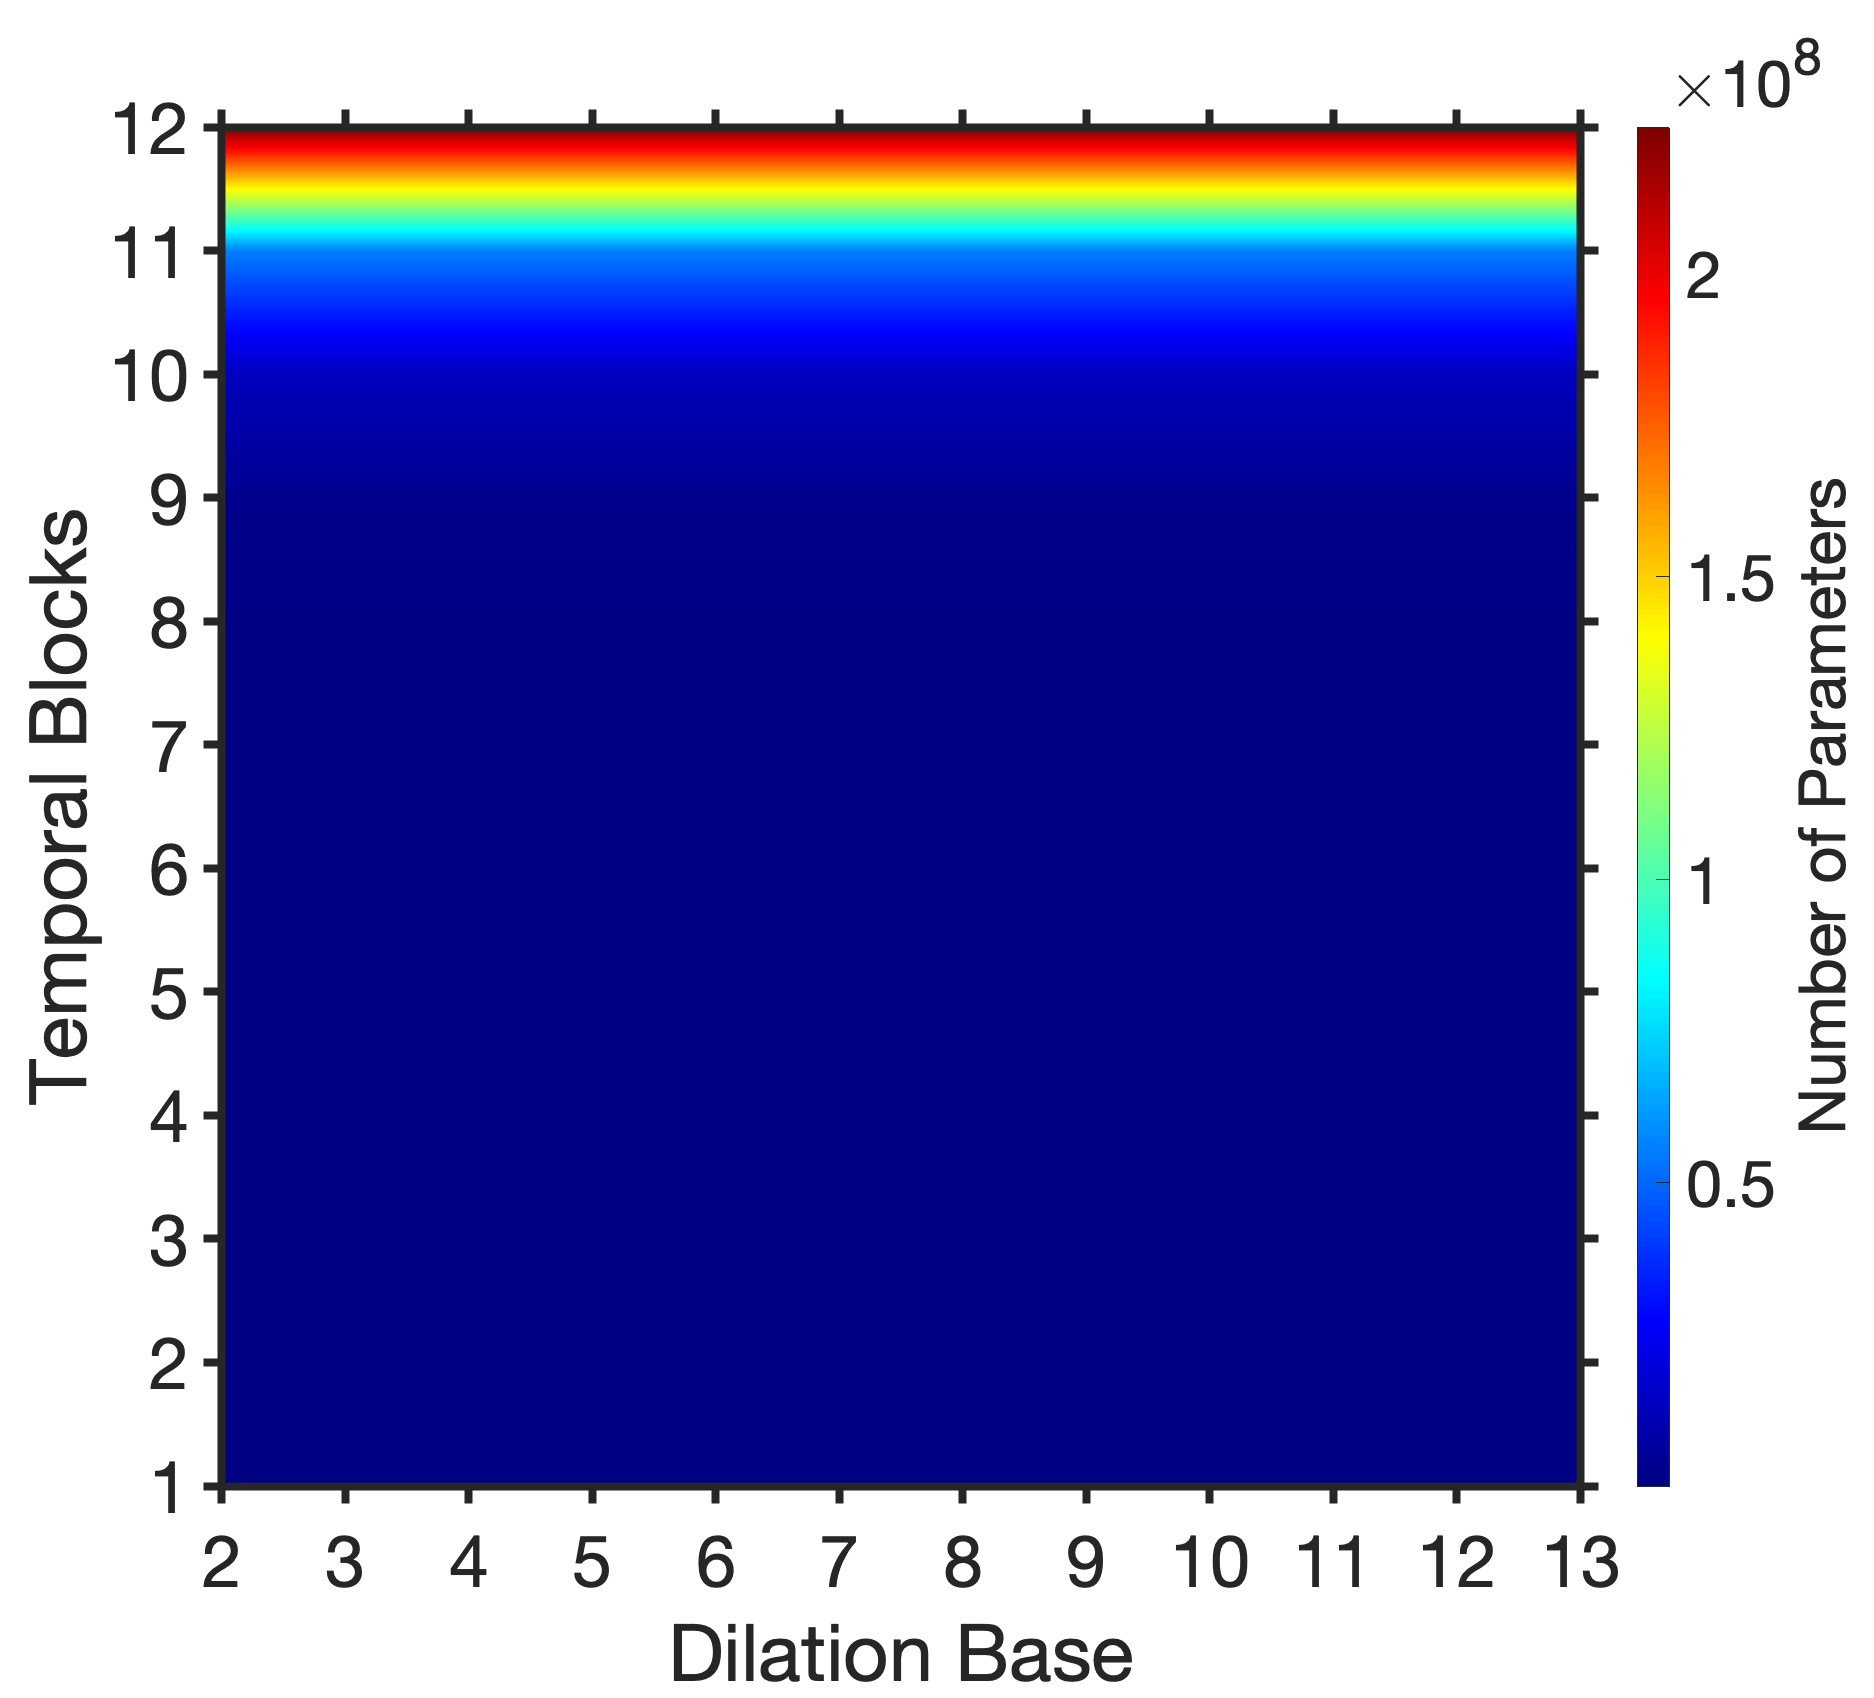
\includegraphics[width=0.28\textwidth]{Figures_manuscript/temp_dil_param.png} &
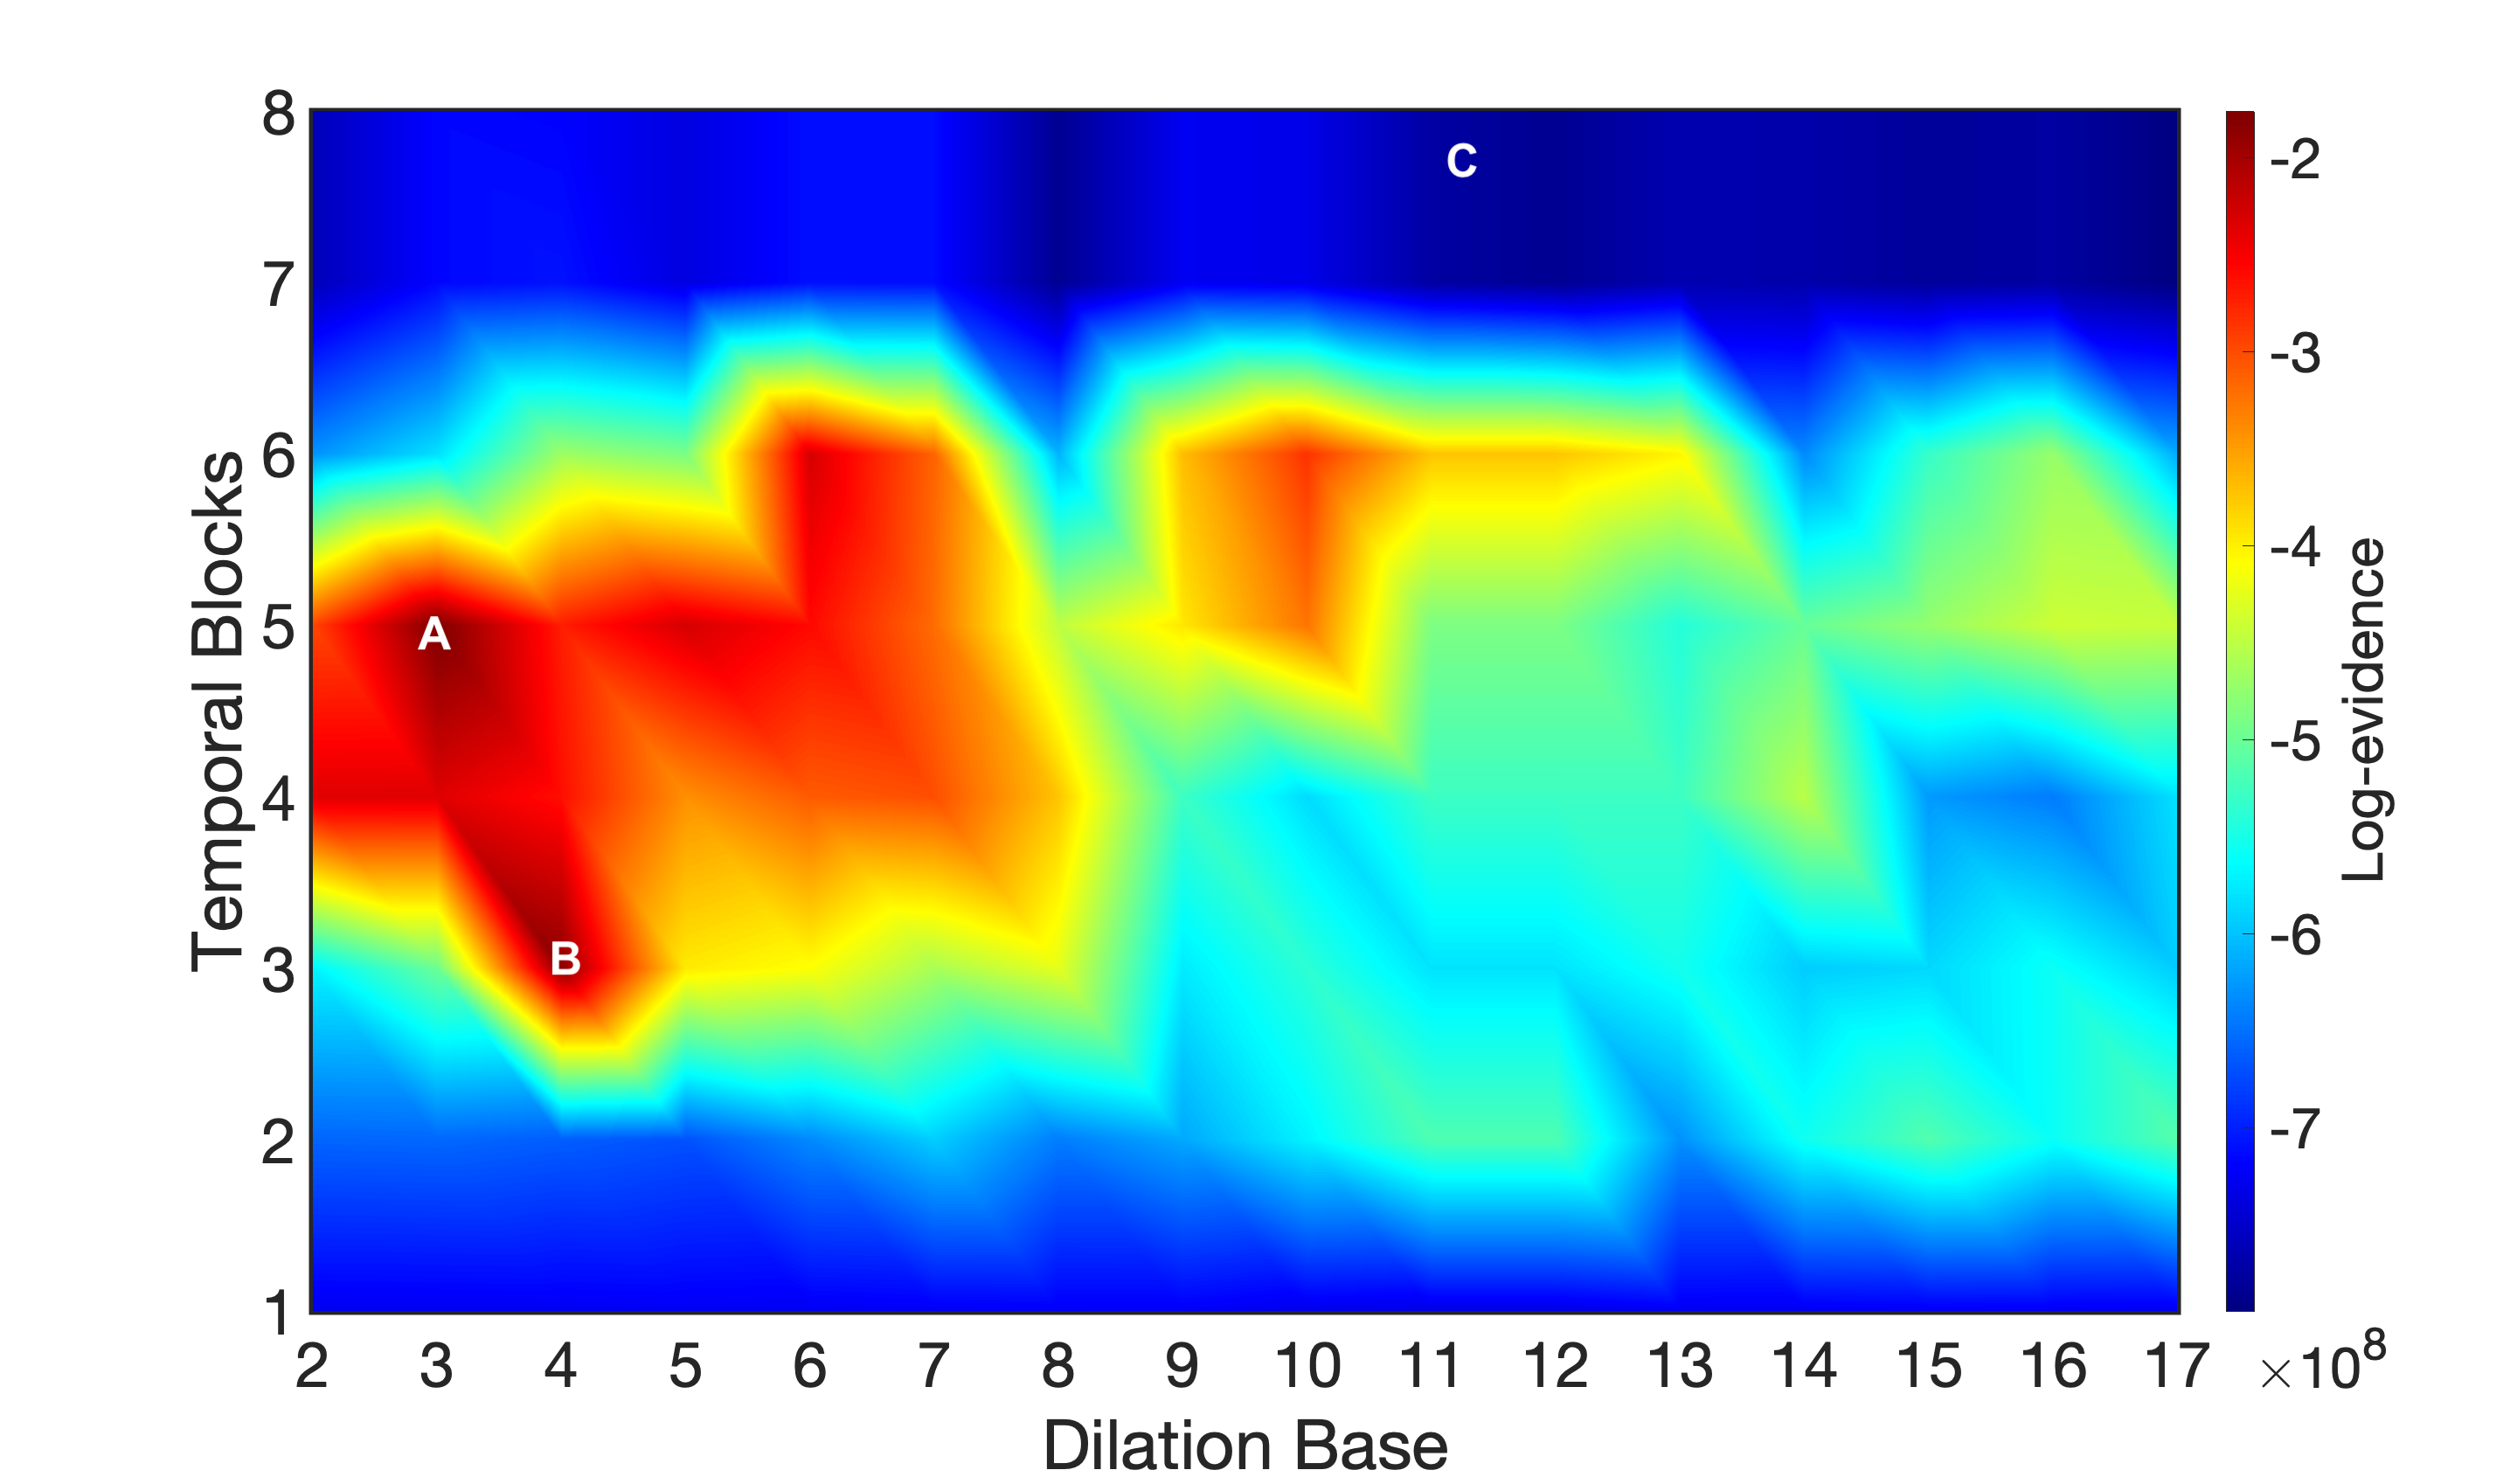
\includegraphics[width=0.45\textwidth]{Figures_manuscript/temp_dil_evid.png}
\\
(a) & (b) & (c)
\end{tabular}
% Bottom row: representative predictions
\begin{tabular}{ccc}
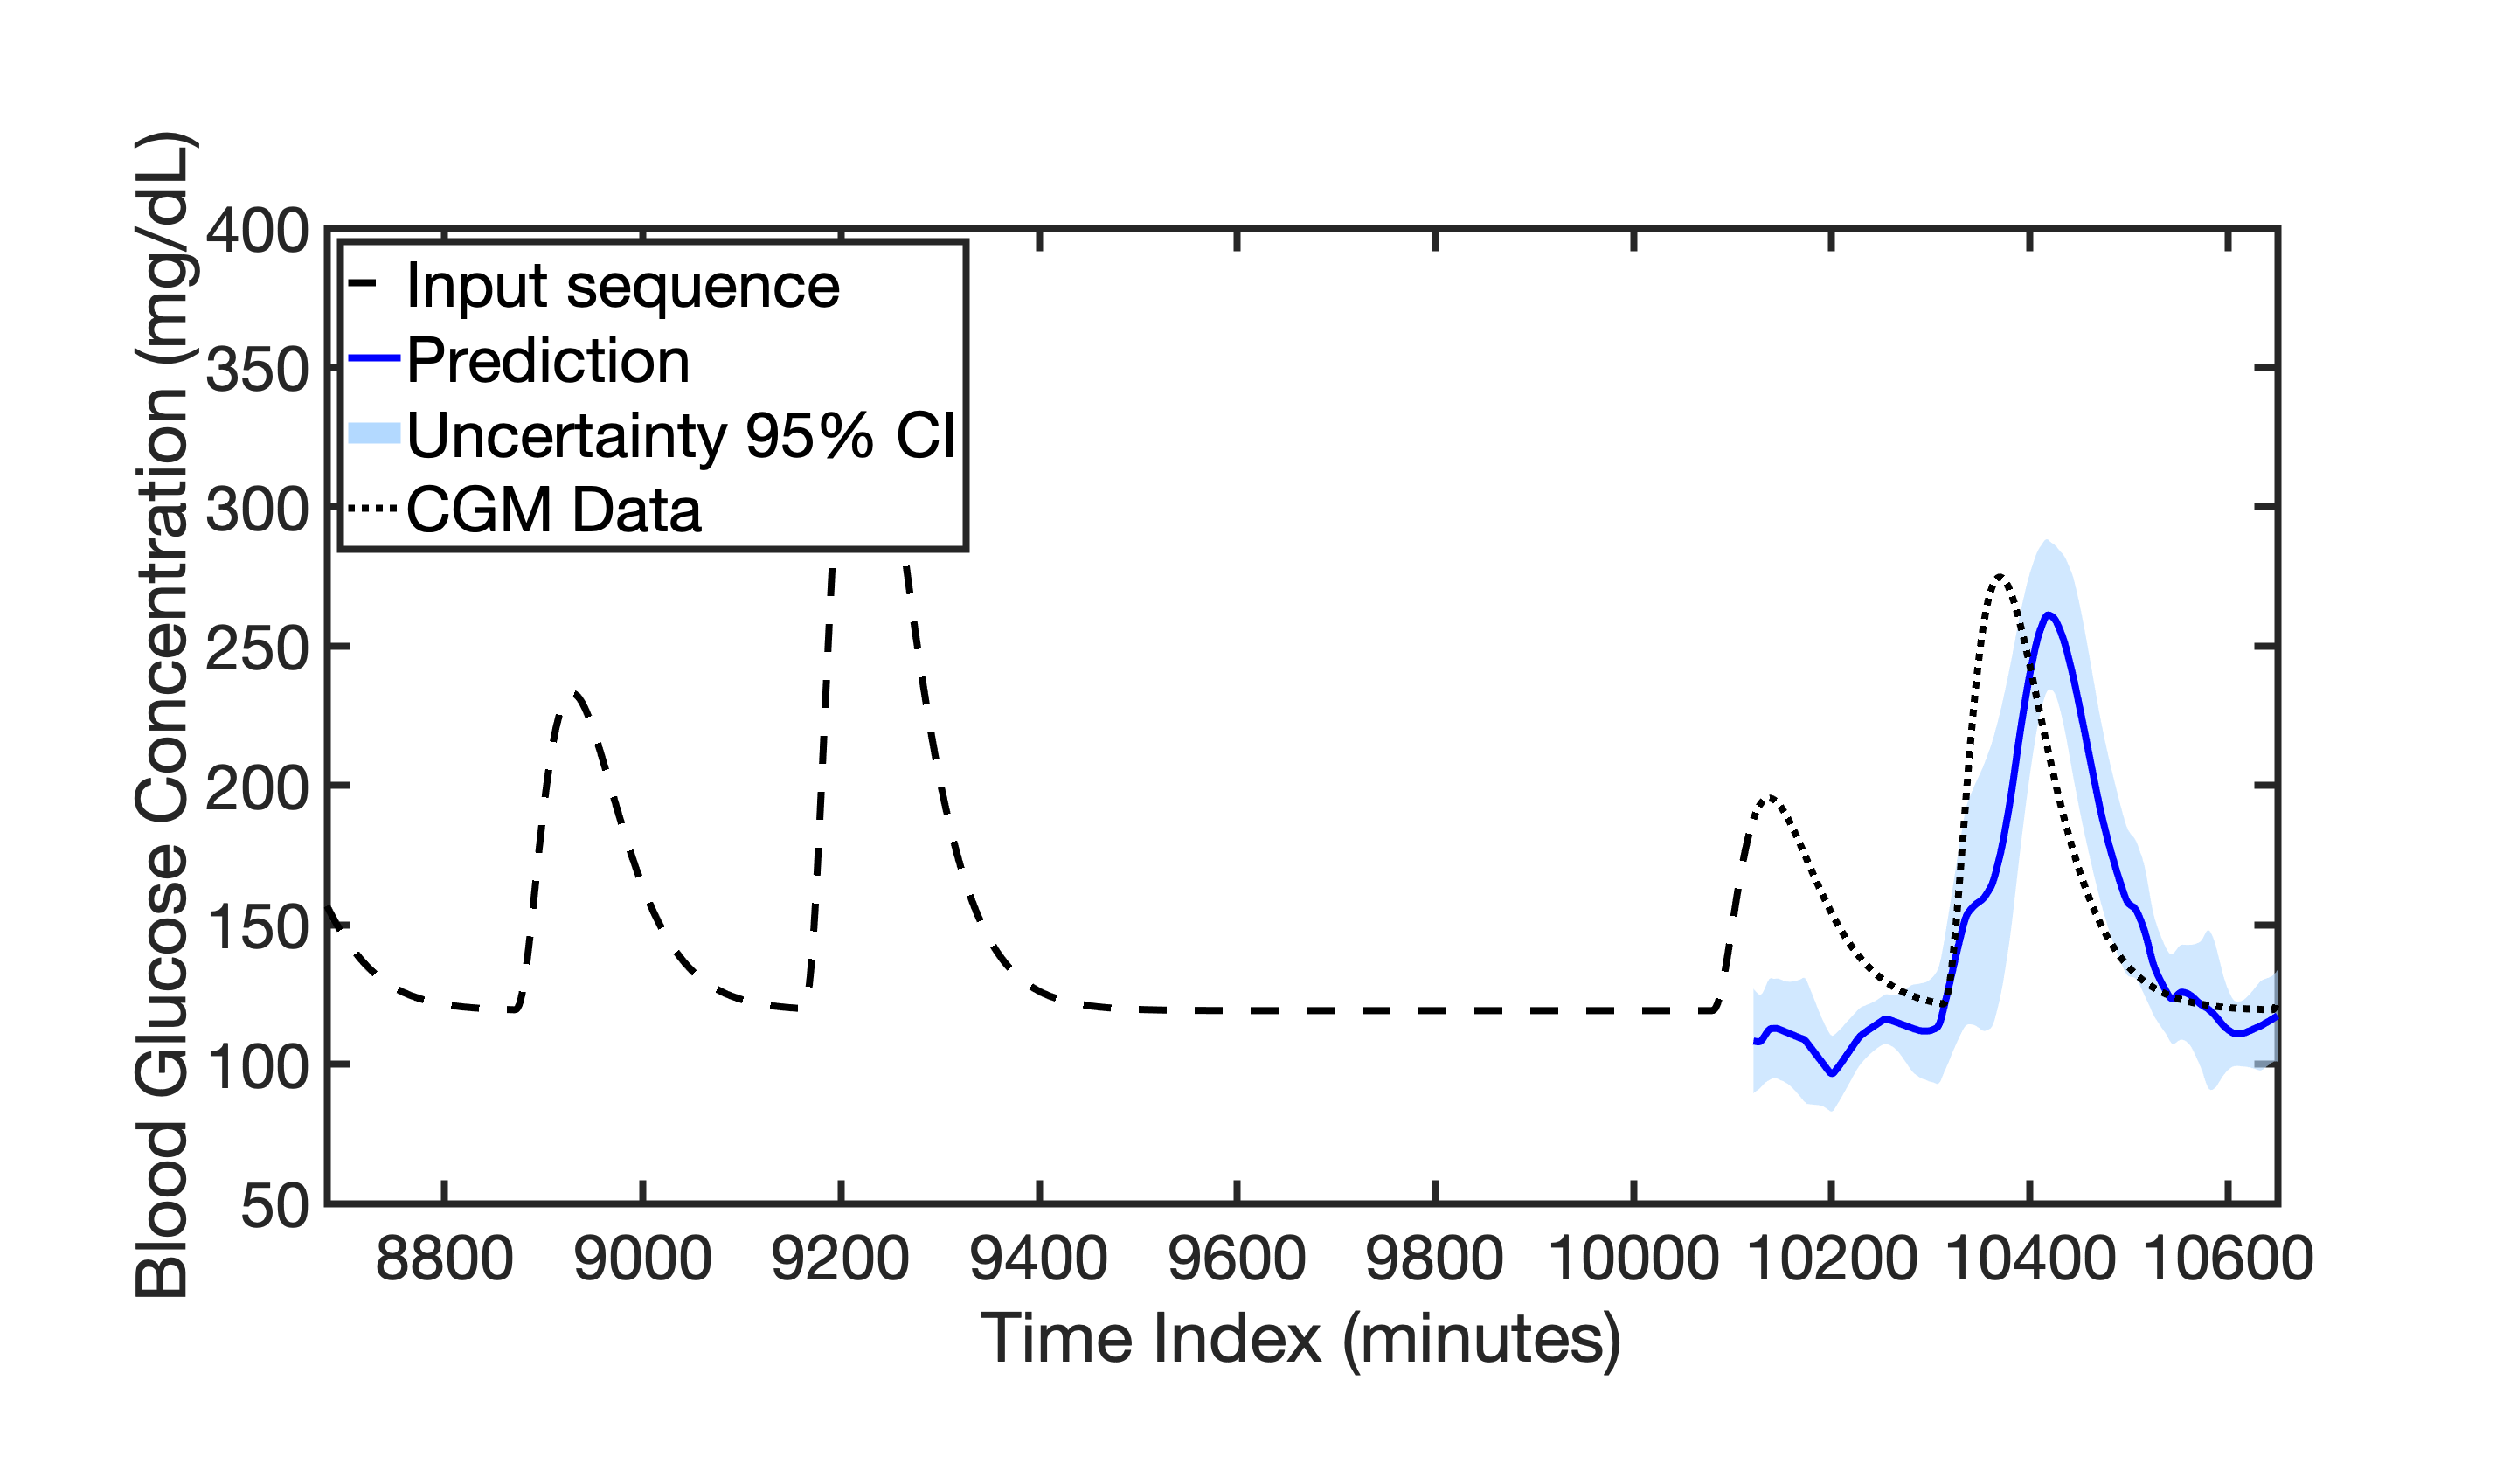
\includegraphics[width=0.30\textwidth]{Figures_manuscript/pred_pointA.png} &
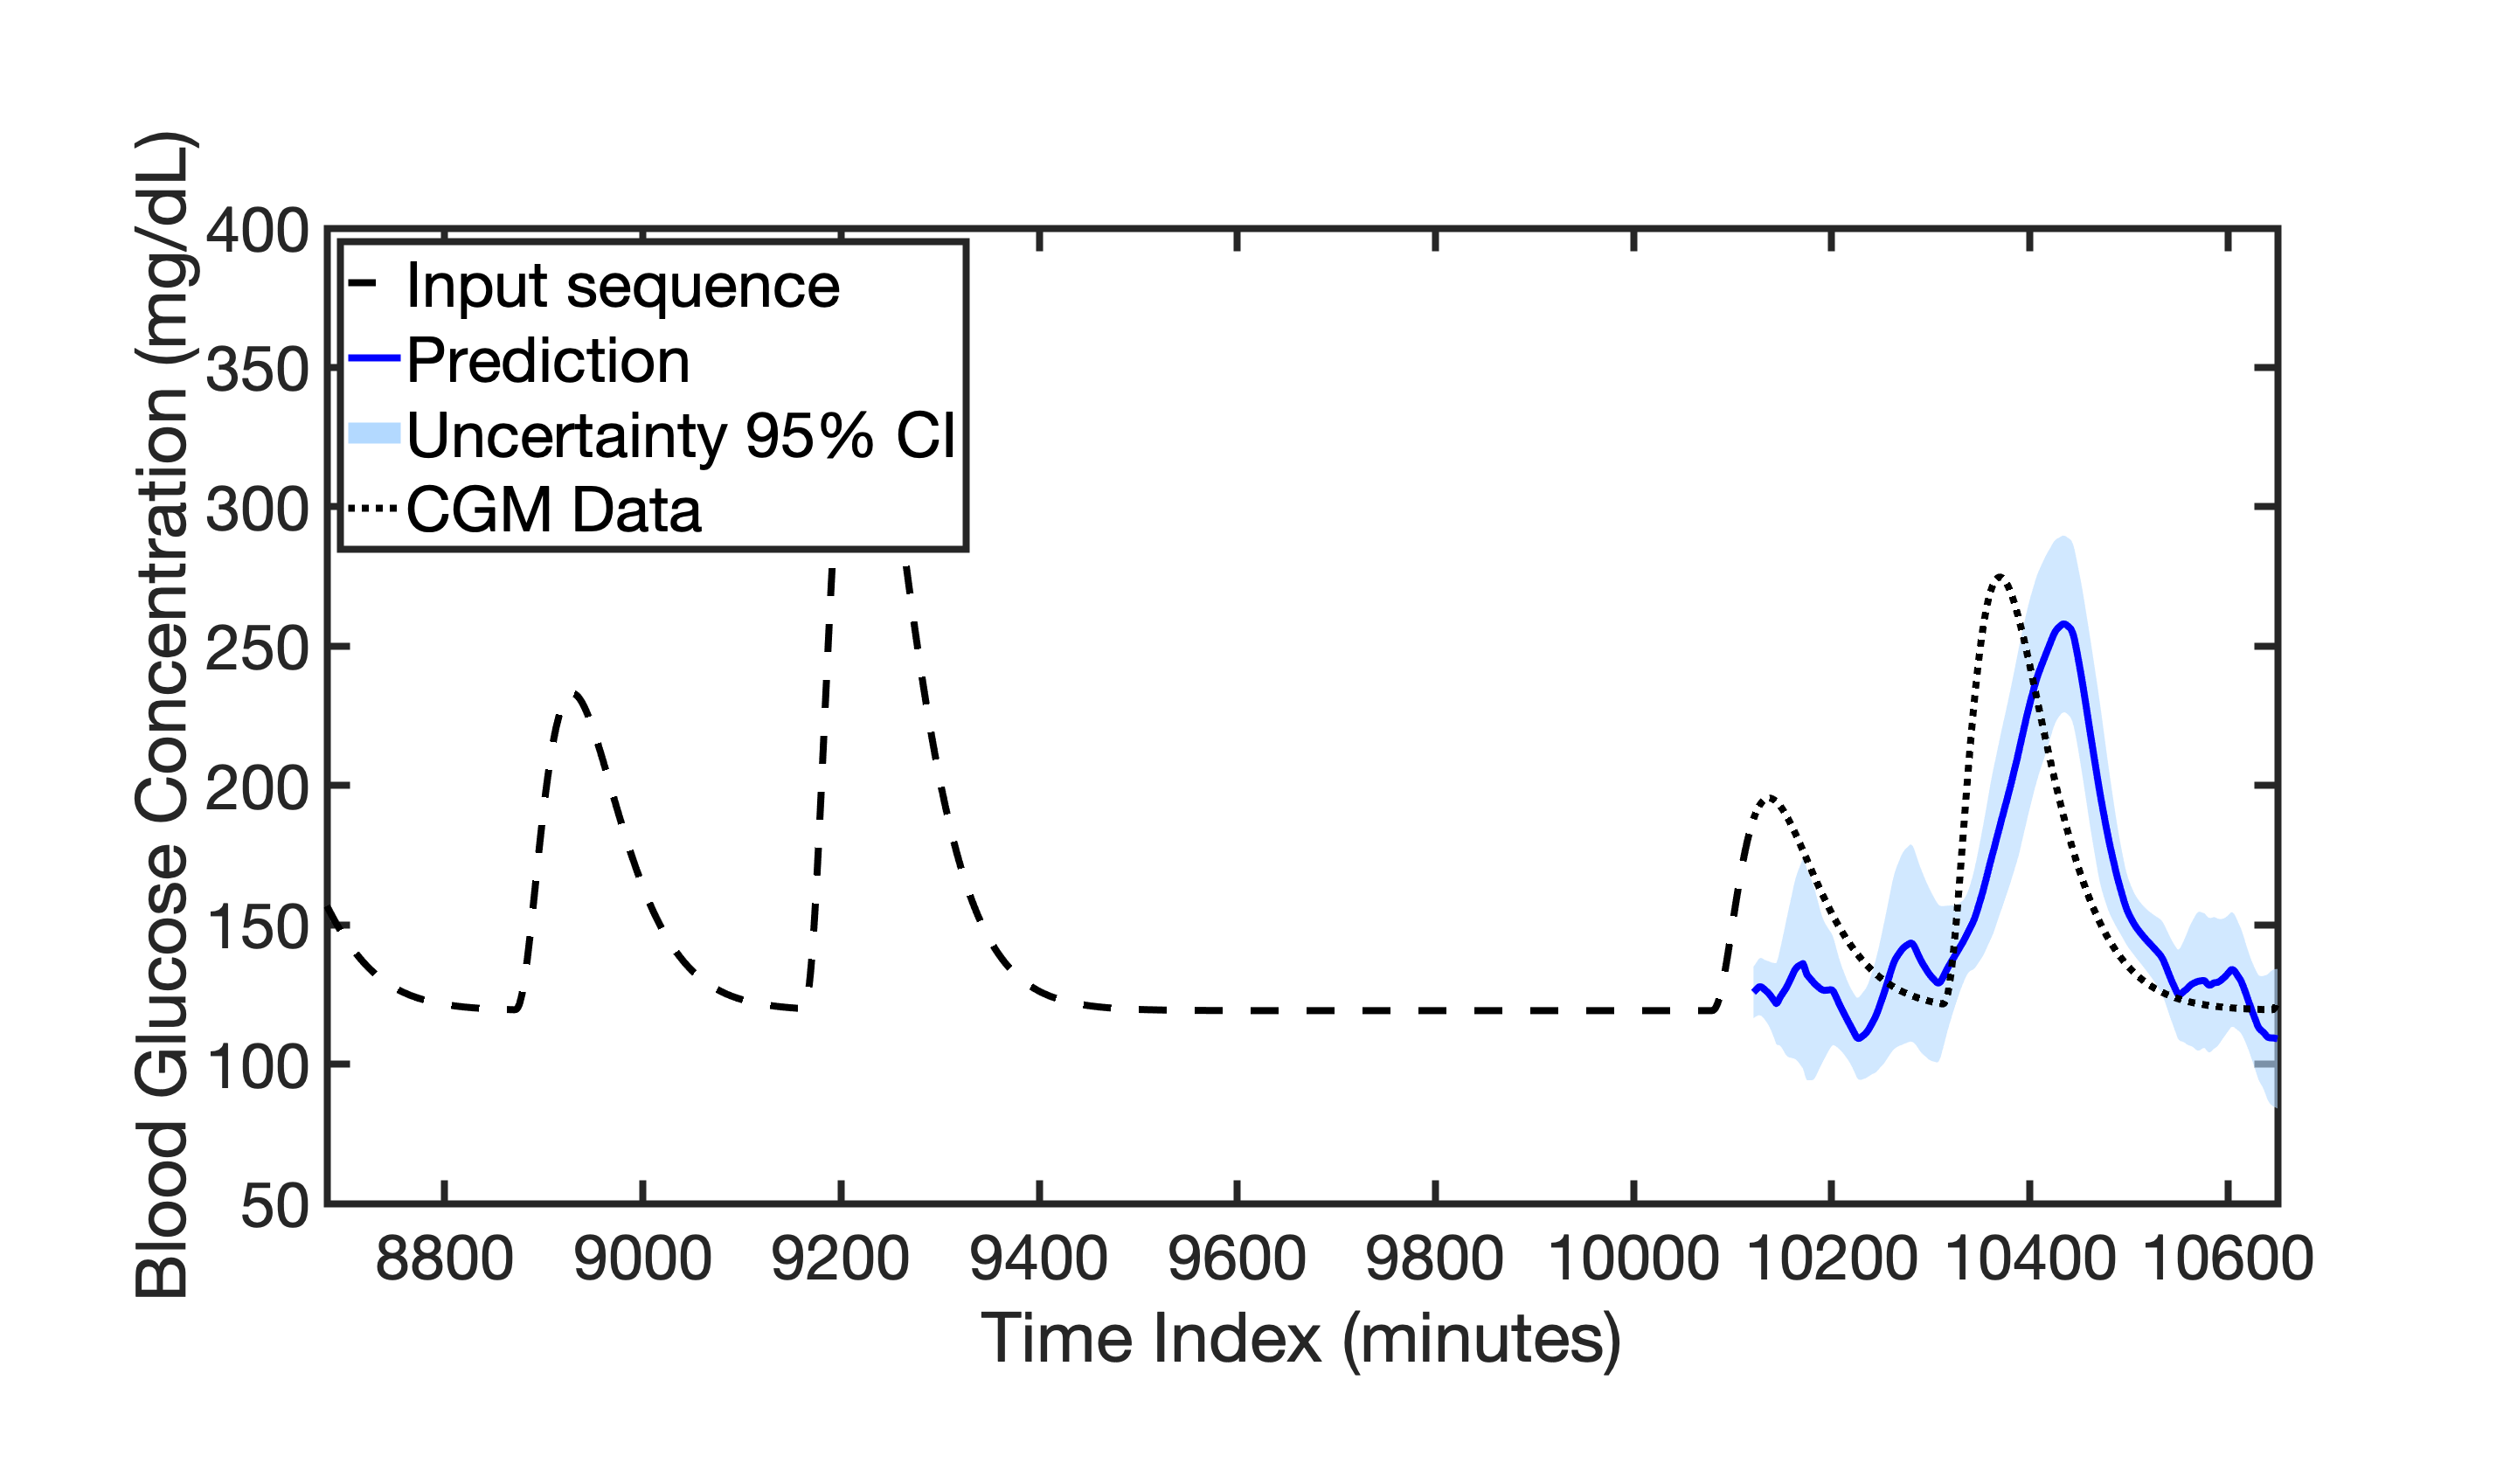
\includegraphics[width=0.30\textwidth]{Figures_manuscript/pred_pointB.png} &
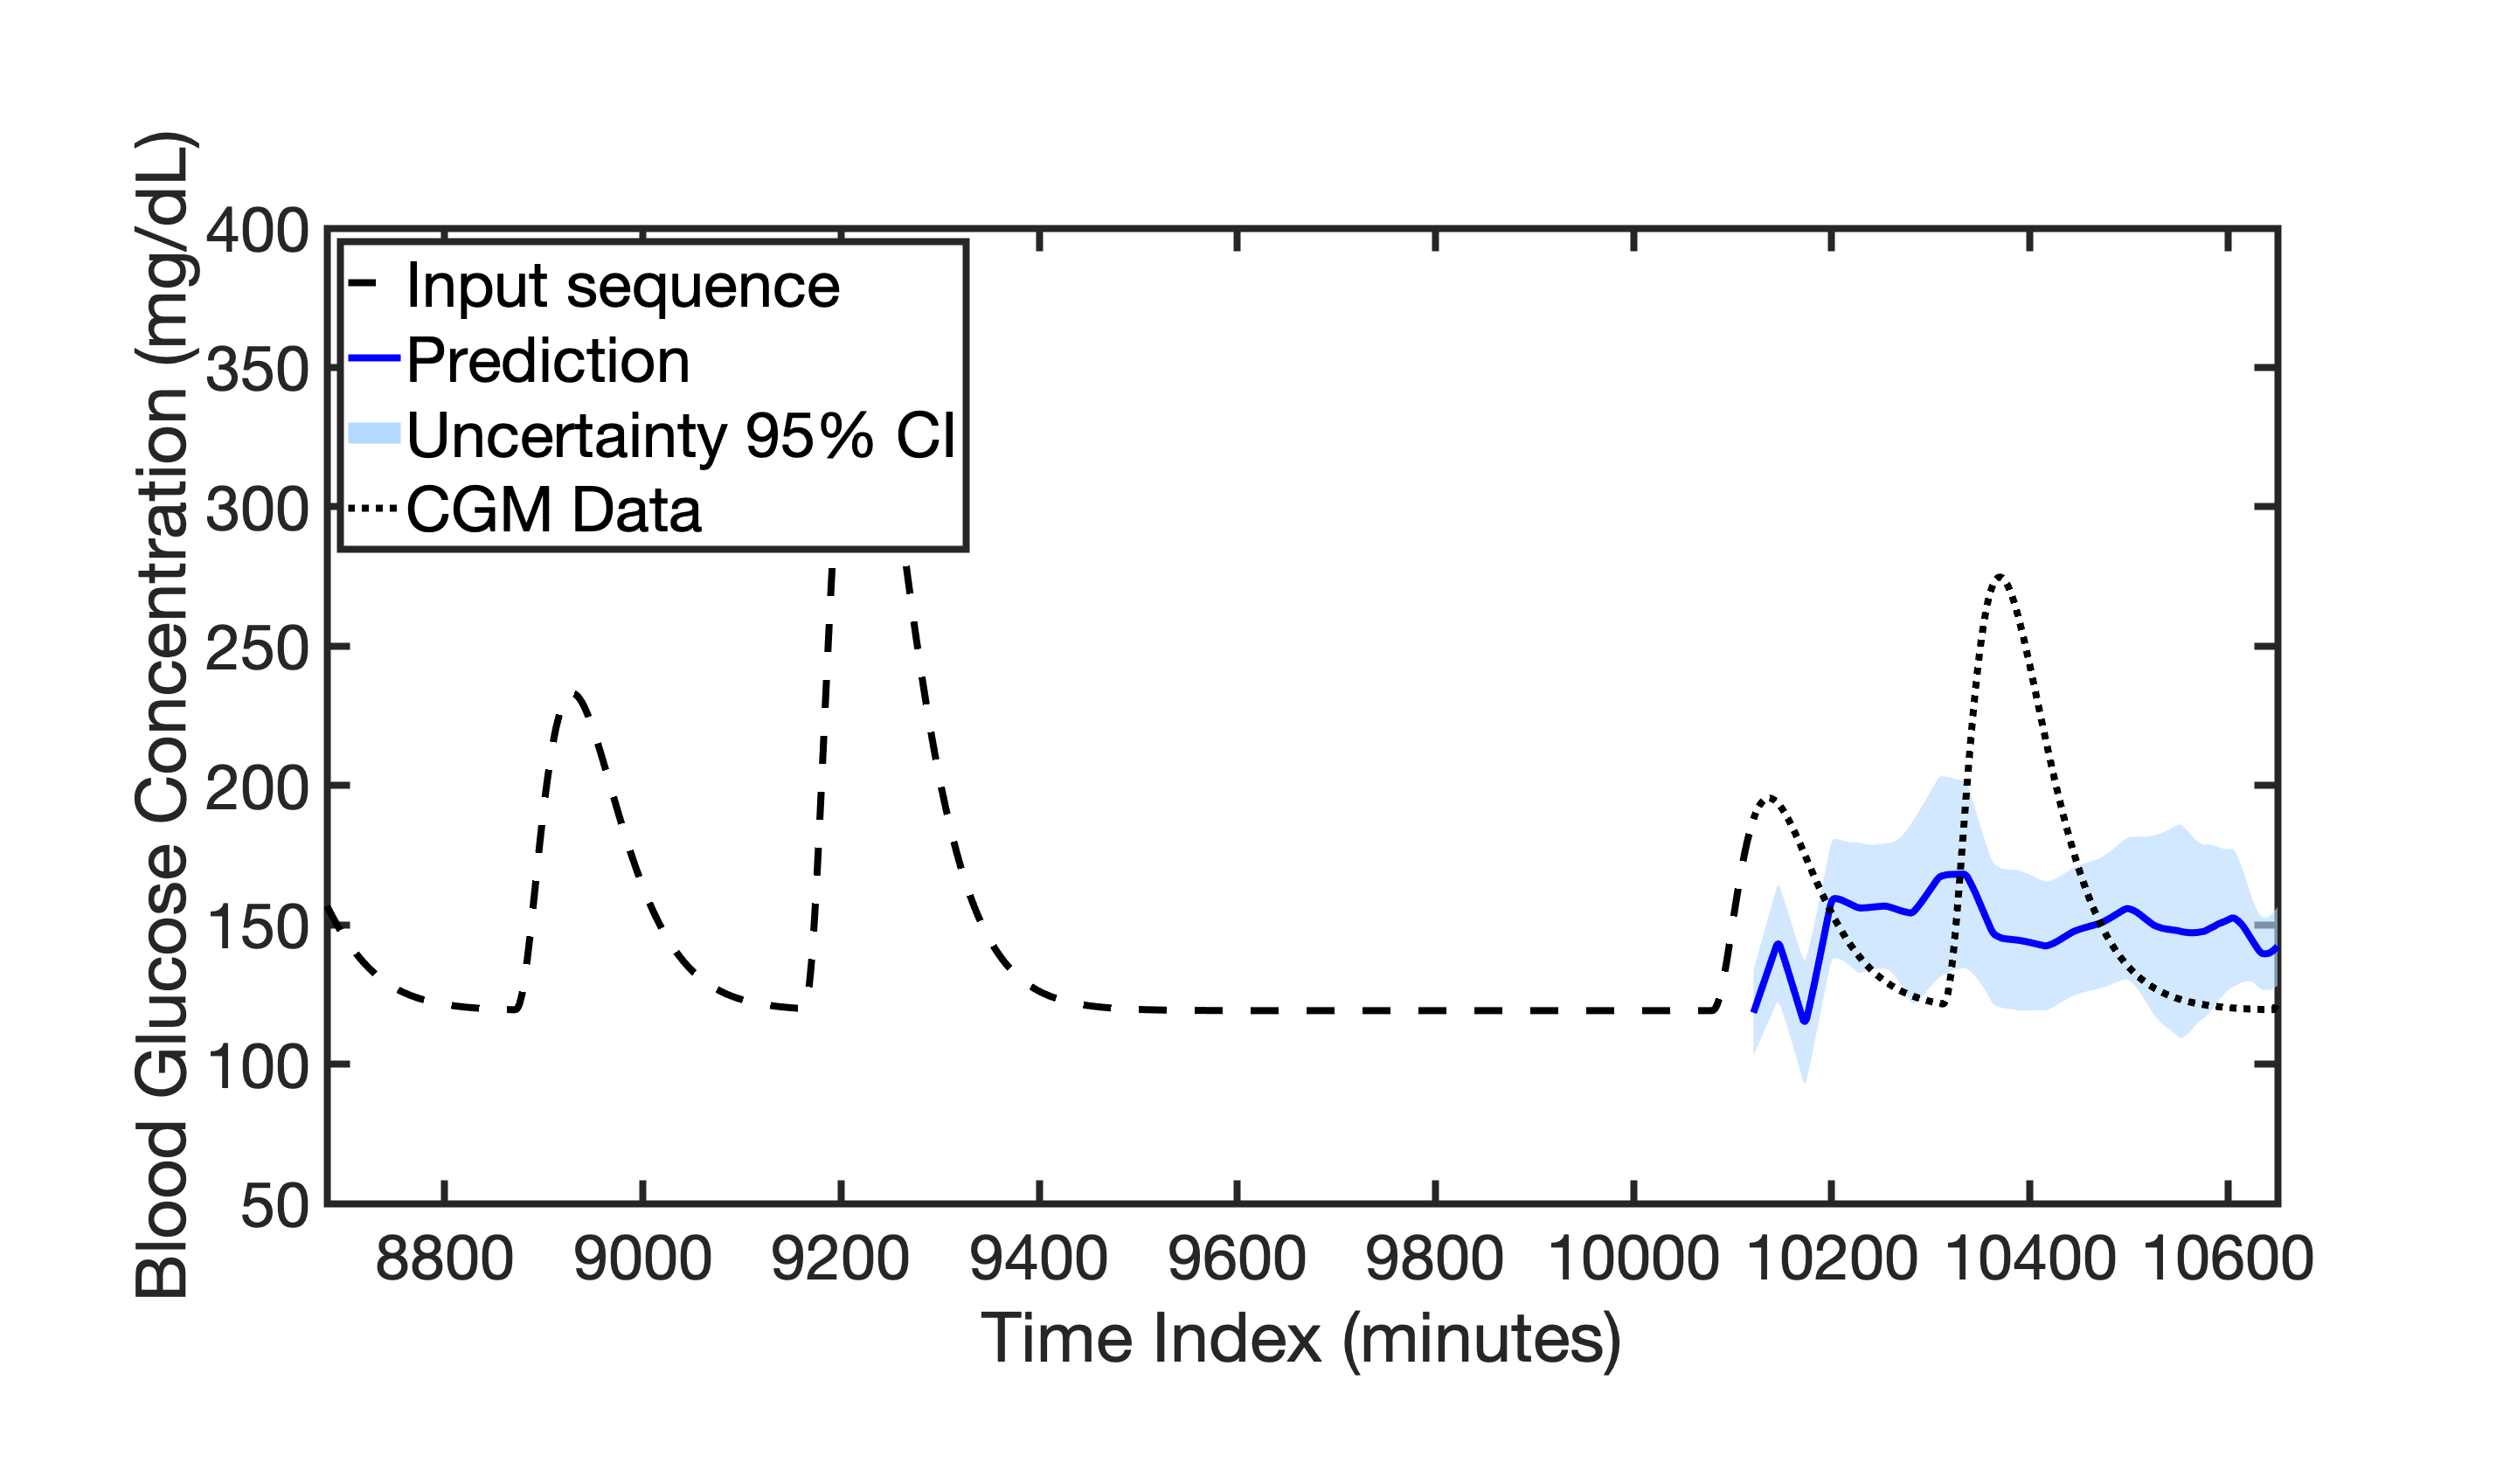
\includegraphics[width=0.30\textwidth]{Figures_manuscript/pred_pointC.png} \\
(d) architecture A & (e) architecture B & (f) architecture C
\end{tabular}

\caption{
Evidence landscape and representative predictive behavior across the TCN architecture space.
(a,b) Receptive field and number of trainable parameters as a function of the number of temporal blocks $N$ and dilation base $b$.
(c) Log-evidence surface over $N$ and $b$, showing a highly non-uniform structure with high-evidence architectures concentrated in an intermediate region of the architecture space.
(d--f) Prediction horizons for representative architectures A, B, and C selected from distinct regions of the evidence landscape in (c). 
In all architectures filter size $f=5$, stride $s=3$, encoder/decoder channels $\{c_j\}=\{\tilde{c}_j\}=\{8\}$ repeated across blocks, input history $d_G=d_M=d_I=1400$~min, and prediction horizon $H=500$~min.
}
\label{fig:dil_evid_pred}
\end{figure}


%
We first examine how Bayesian evidence varies across TCN architectures with different receptive fields and model capacities. 
Figure~\ref{fig:dil_evid_pred}(a and b) show that both the number of temporal blocks \(N\) and the dilation base \(b\) increase the receptive field, while model size, measured by the number of trainable parameters, is primarily driven by \(N\). 
%
The evidence landscape of the 136 architectures in Figure~\ref{fig:dil_evid_pred}(c) is highly non-uniform, with high-evidence models concentrated in an intermediate region of the \((N,b)\) architecture space. This indicates that neither larger receptive fields nor larger model sizes alone improve model plausibility. Instead, evidence favors architectures that provide sufficient temporal context to capture meal and insulin dynamics while avoiding weakly informed parameters.
%
The forecast behavior of three representative architectures (A, B, and C) from different regions of the architecture space is shown in Figure~\ref{fig:dil_evid_pred}(d--f). Architectures A and B, located in high-evidence regions, produce accurate forecasts with tighter uncertainty bands. In contrast, architecture C, selected from a low-evidence region, yields less reliable predictions despite its larger number of temporal blocks. These results suggest that evidence is not merely measuring goodness-of-fit, but also identifying architectures with improved predictive reliability under uncertainty.

%


% -- Evidence vs stride/input/output
\begin{figure}[!ht]
\centering
\setlength{\tabcolsep}{4pt}
\renewcommand{\arraystretch}{1.0}
% ==================== TOP BLOCK: STRIDE ====================
\begin{tabular}{ccc}
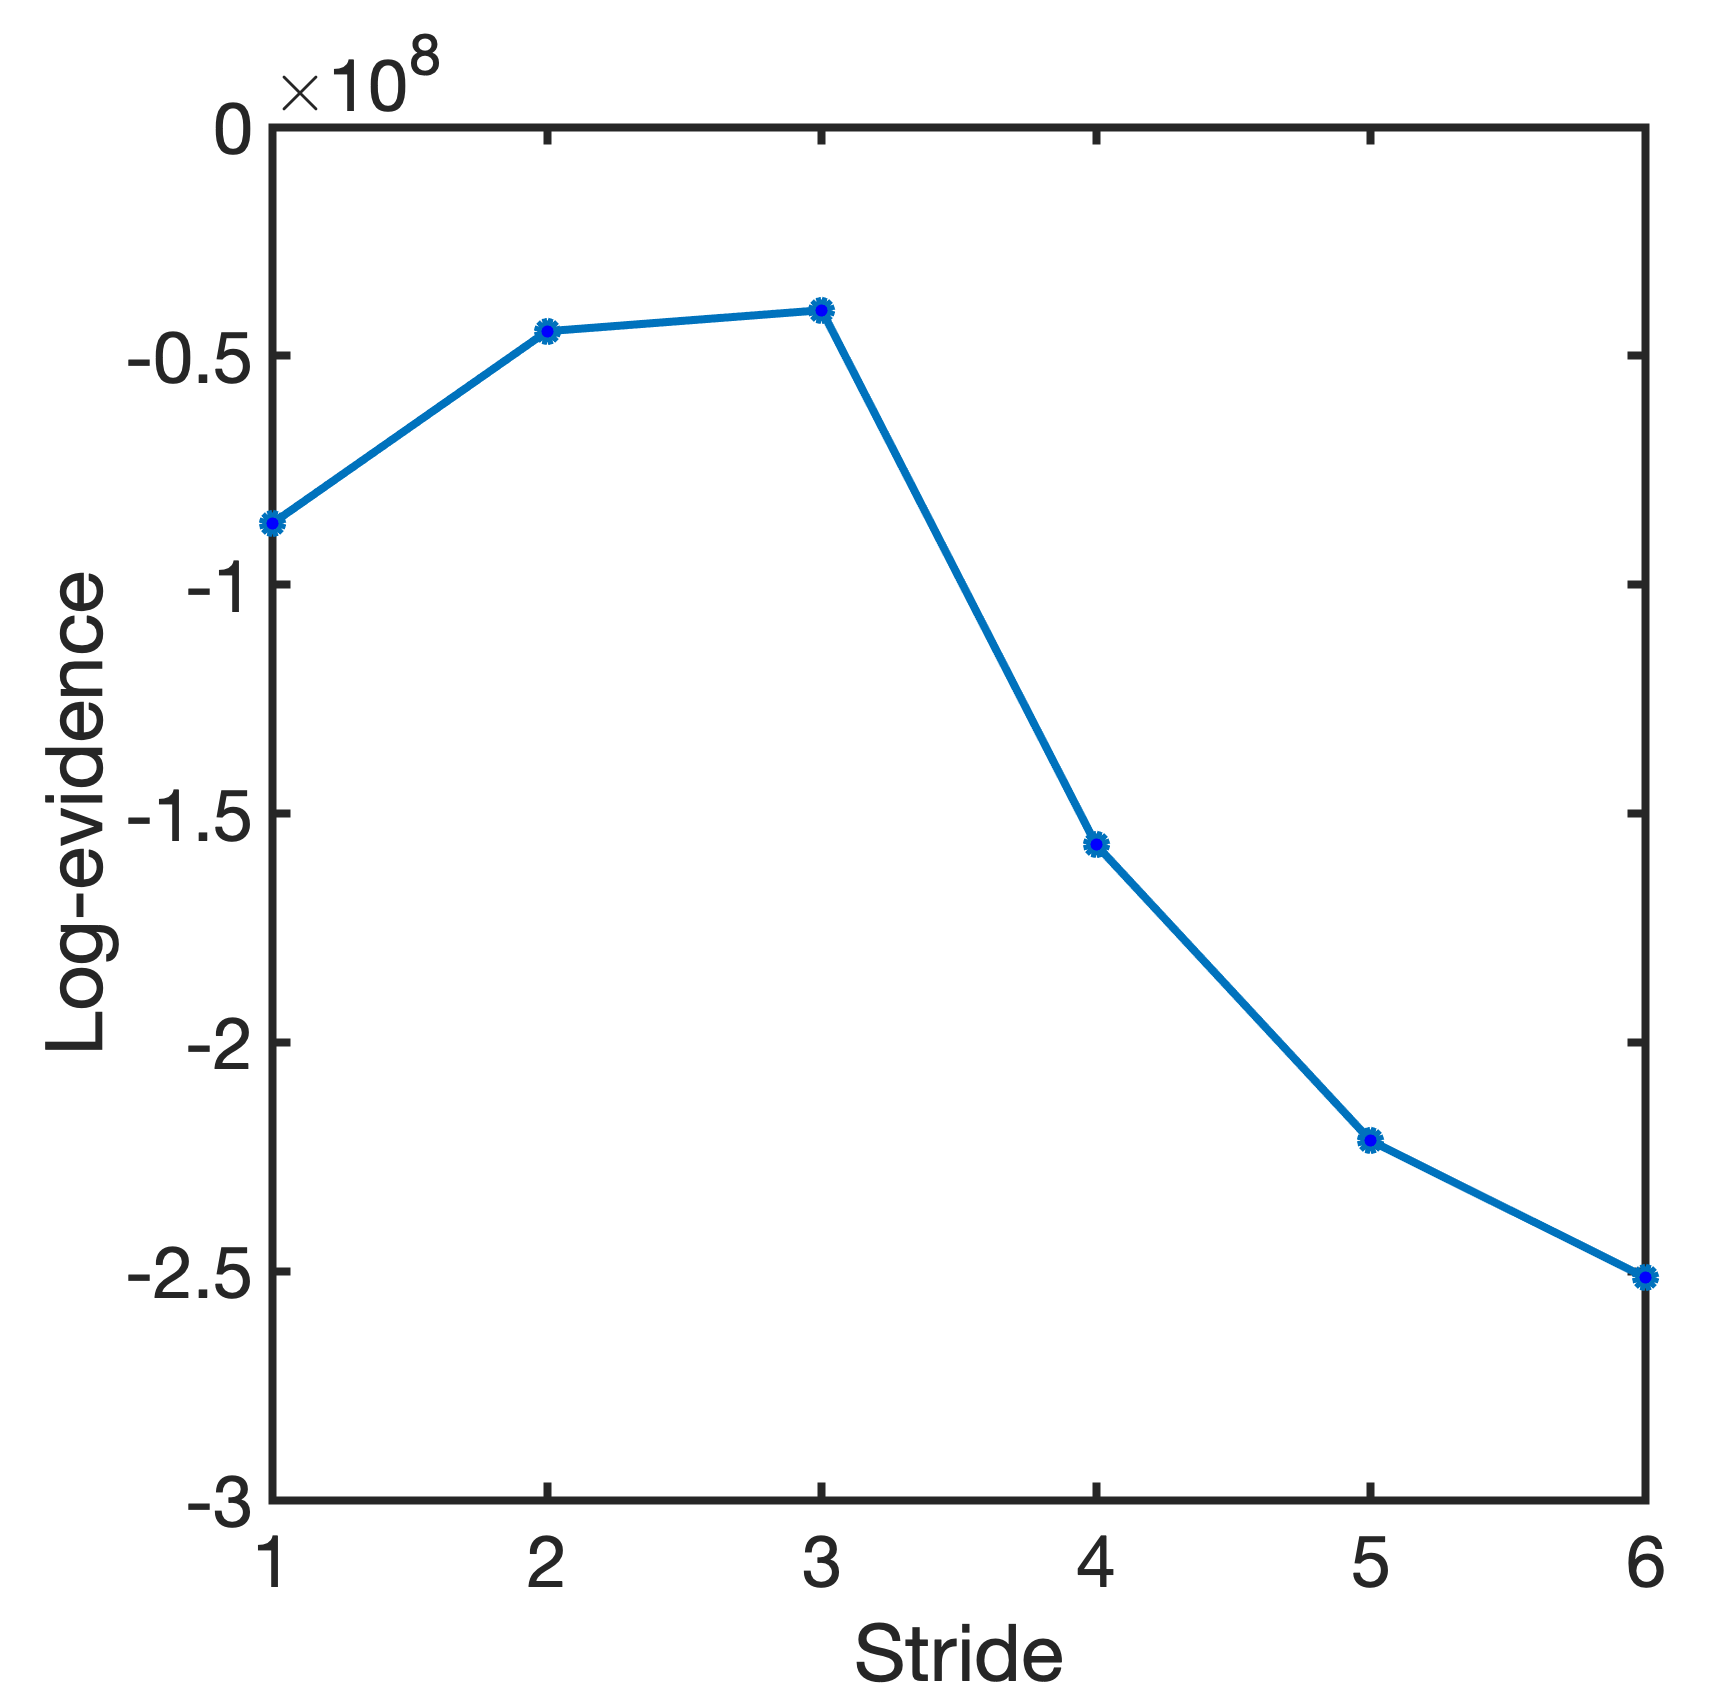
\includegraphics[width=0.323\textwidth]{Figures_manuscript/stride_vs_evid.png} &
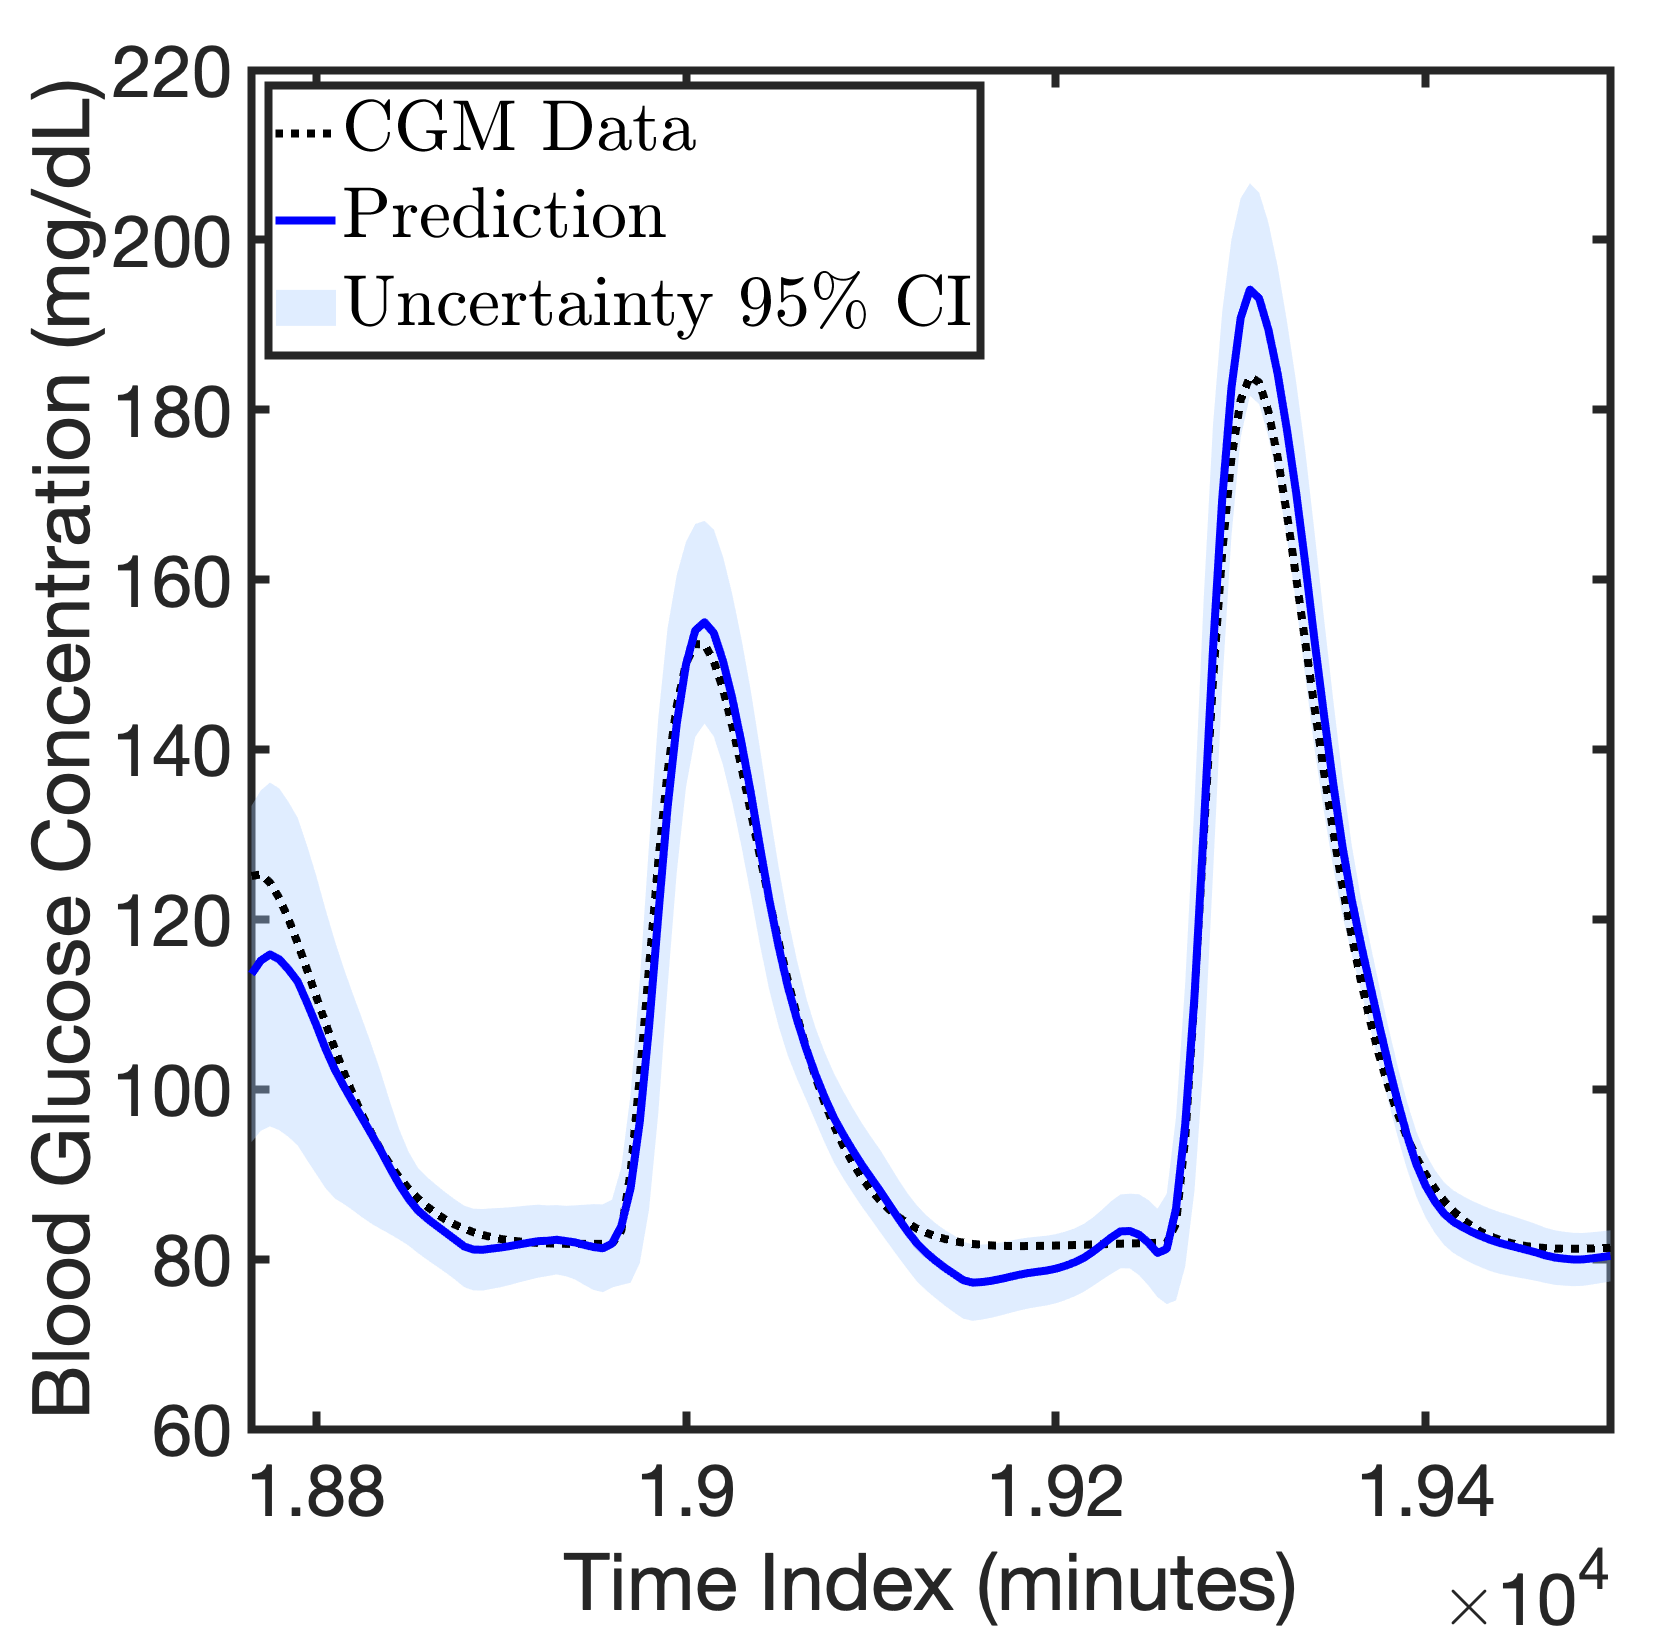
\includegraphics[width=0.31\textwidth]{Figures_manuscript/stride_3.png} &
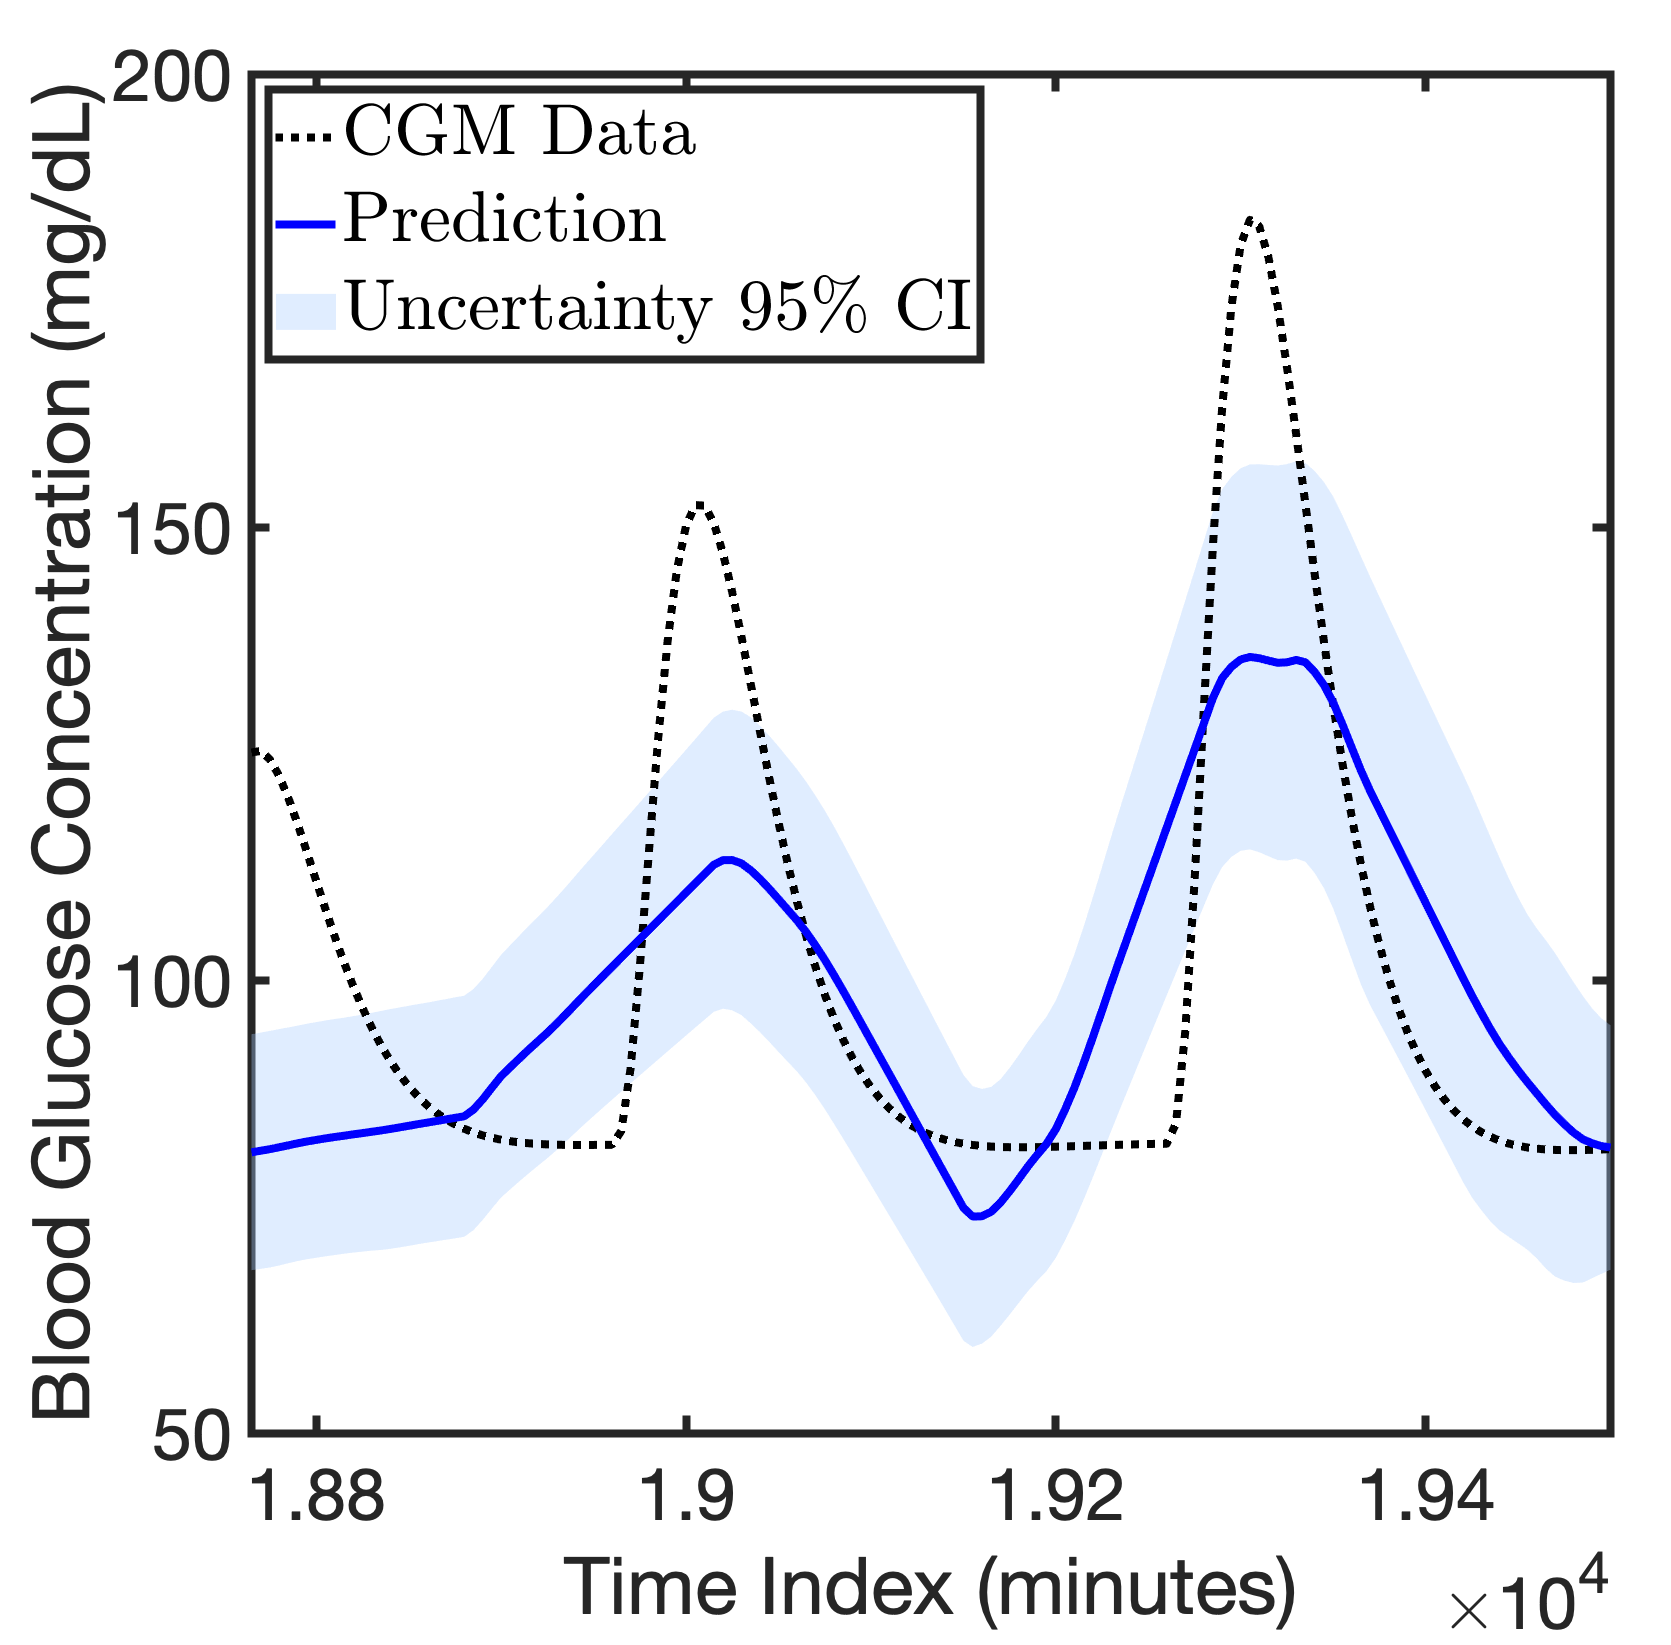
\includegraphics[width=0.31\textwidth]{Figures_manuscript/stride_6.png} \\
(a) & (b) $s=3$ & (c) $s=6$
\end{tabular}
% ==================== BOTTOM BLOCK: INPUT-OUTPUT ====================
\begin{tabular}{c}
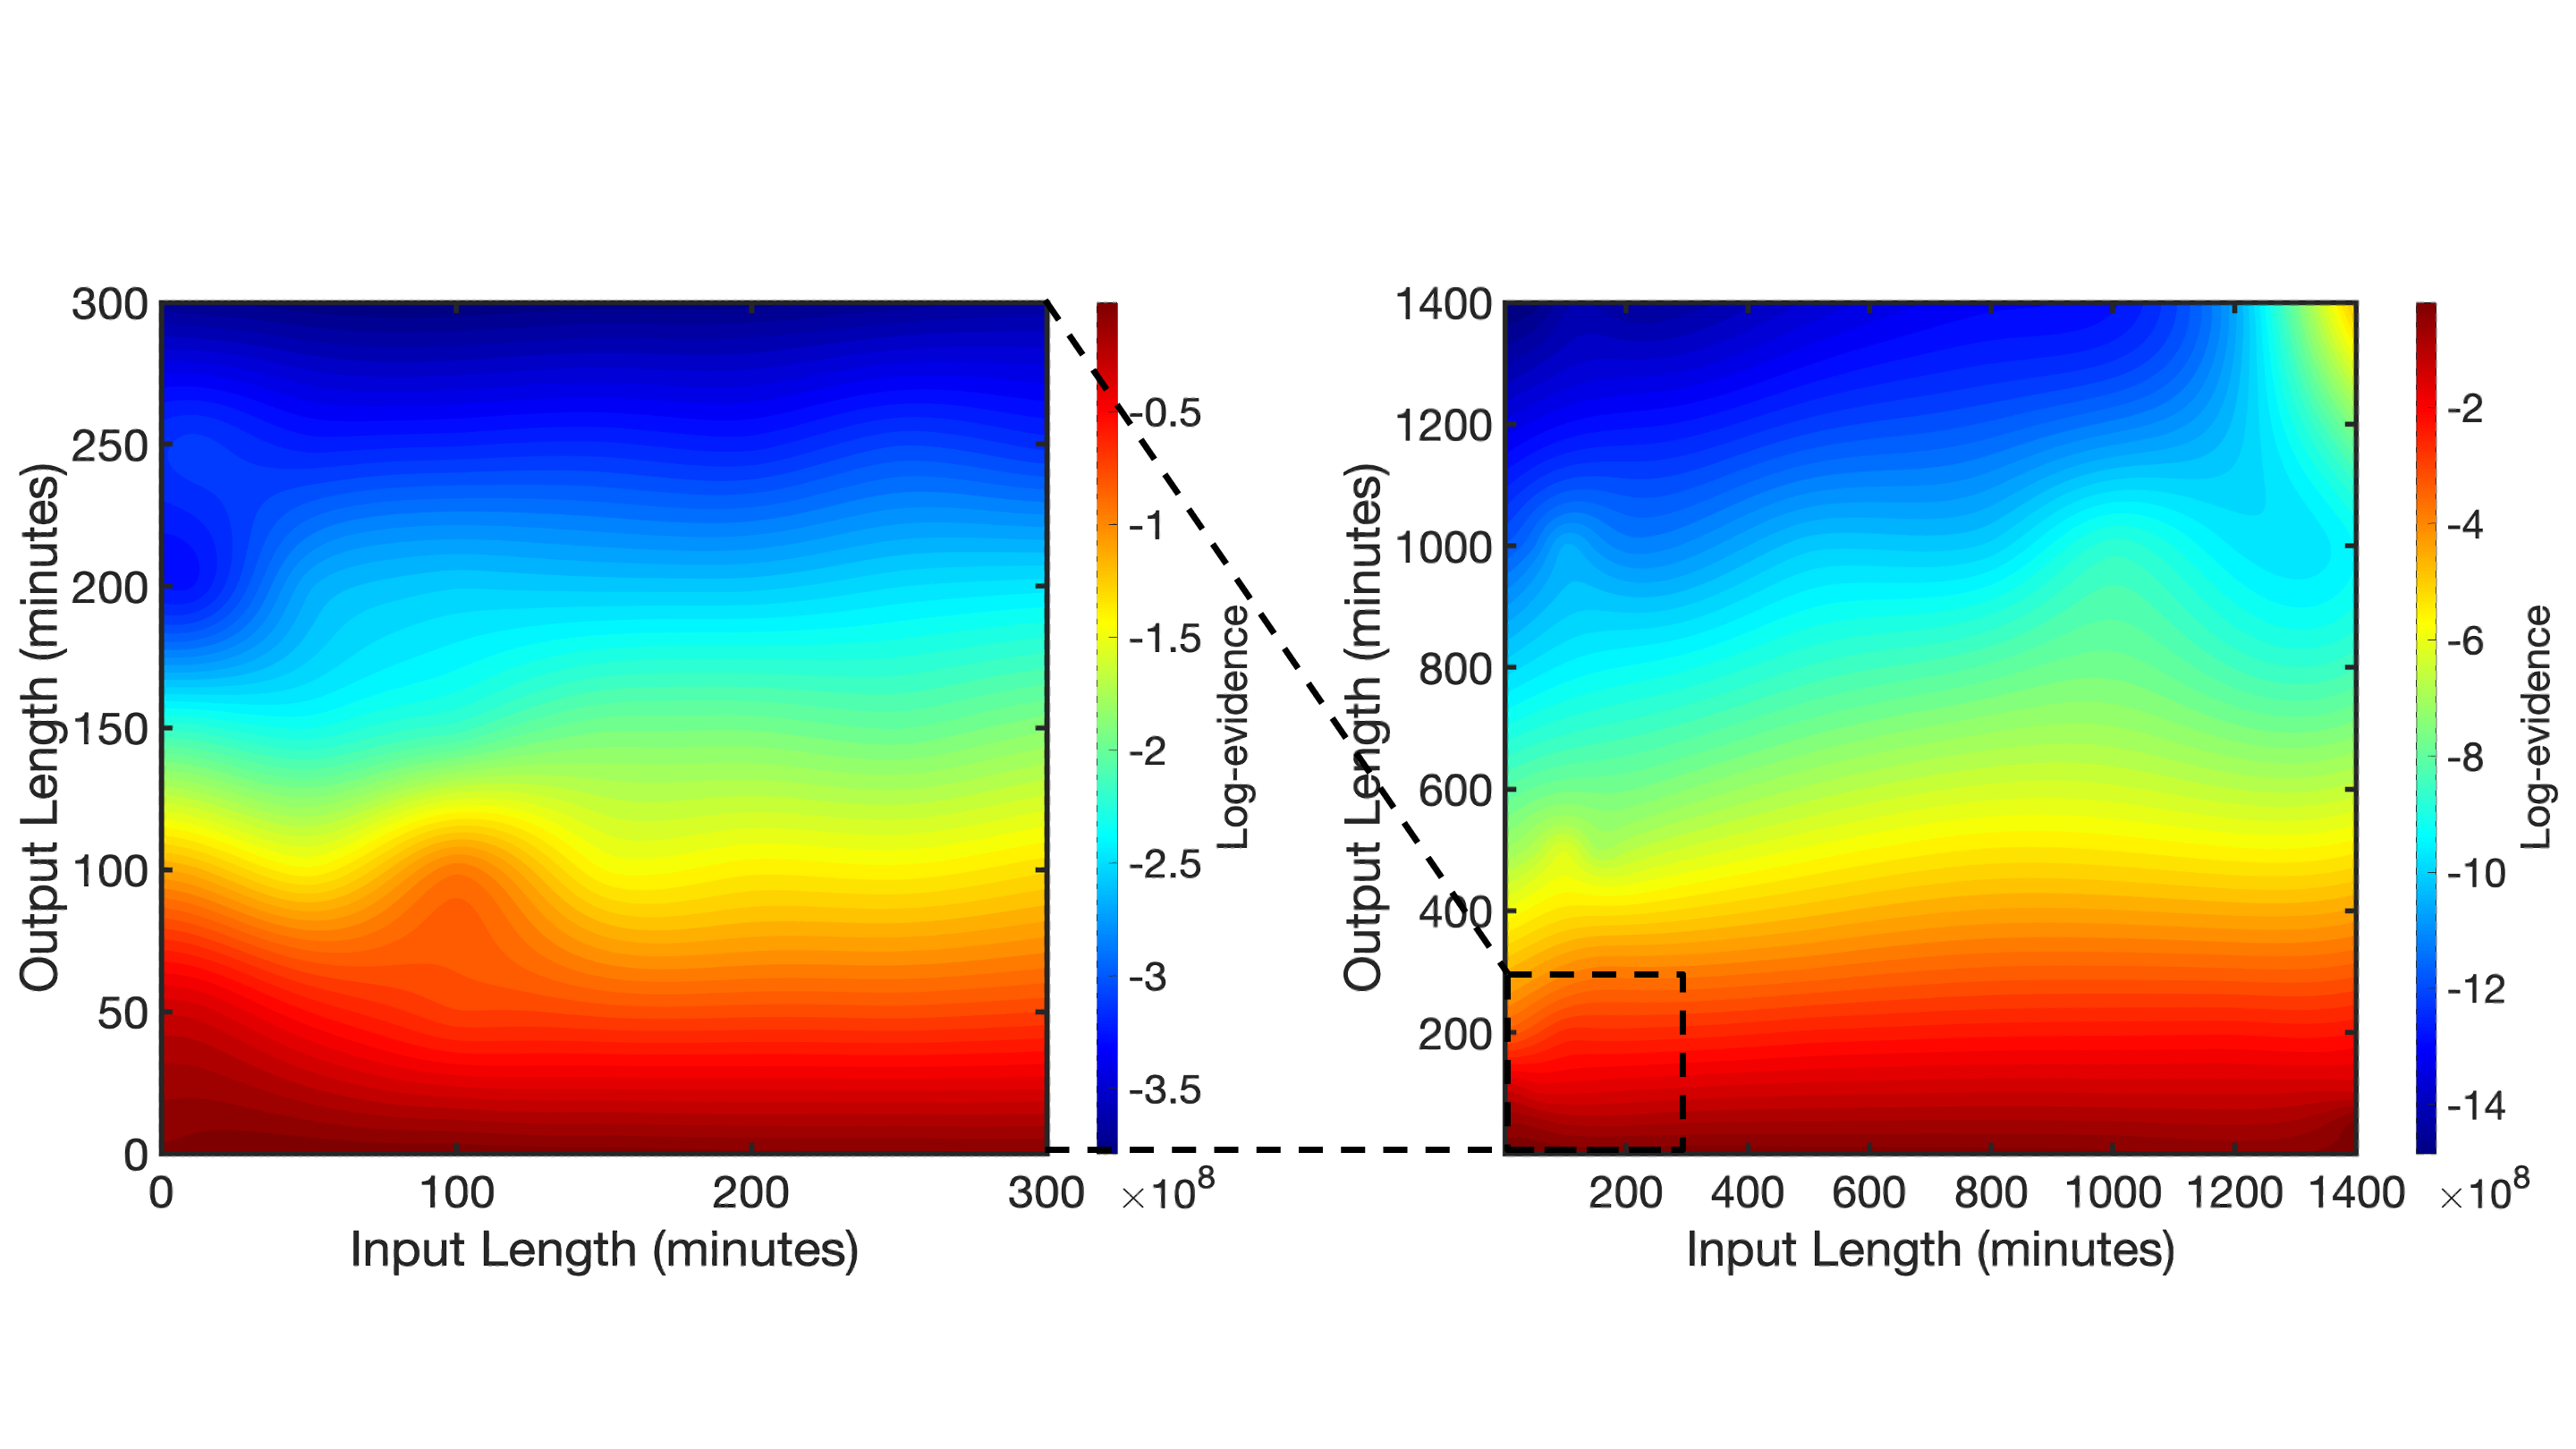
\includegraphics[width=0.78\textwidth]{Figures_manuscript/input_output.png} \\
(d)
\end{tabular}

\caption{ 
(a) Log-evidence as a function of the stride $s$ used to construct overlapping input--output windows for TCN training, showing that an intermediate stride provides the highest evidence. 
(b--c) Representative predictions for stride values $s=3$ and $s=6$. 
(d) Log-evidence surface over input history length $d_G=d_M=d_I$ and prediction horizon $H$; the coarse search over 1400 minutes localizes a high-evidence region, which is refined using a finer grid over the highlighted 300 minute region. 
For all panels, the TCN architecture is fixed at $N=4$ temporal blocks, filter size $f=5$, dilation base $b=3$, and encoder/decoder channels $\{c_j\}=\{\tilde{c}_j\}=\{12\}$. For (a--c), the input history and prediction horizon are fixed at $d_G=d_M=d_I=1400$~min and $H=1000$~min; for (d), the stride is fixed at $s=3$.
}
\label{fig:stride_inputoutput}
\end{figure}


In addition to architecture’s structural parameters, evidence also provides guidance for training and forecasting choices in TCN. Figure~\ref{fig:stride_inputoutput}(a-c) shows the effect of stride in constructing overlapping input–output windows and the evidence surface over input length $d$ and prediction horizon $H$. The evidence peaks at stride $s=3$, indicating a balance between highly redundant training windows at small stride and reduced sample efficiency at large stride. This suggests that evidence also captures the effective information content of the training set induced by the windowing training scheme.
Figure~\ref{fig:stride_inputoutput}(d) shows that evidence decreases as the prediction horizon increases, indicating that longer-horizon forecasts are less supported by the available data. For a fixed horizon, the evidence surface also localizes a favorable range of input history lengths rather than increasing monotonically with longer input windows. To identify this region efficiently, we first evaluate a coarse grid over input and output lengths and then refine the high-evidence region using a finer search. Overall, the results of this section show that evidence can be used to identify both the structural specification of TCN architecture and the temporal configuration of the forecasting problem. 


%++++++++++++++++++++++++++++++++++++++++++++++++++++++++++++++++++++++++
\subsection{EVIDENT for population-level TCN architecture discovery}\label{sec:evident_results}

We now implement EVIDENT in a clinical forecasting setting involving inter-patient variability and data noise from CGM sensor. The objective is to leverage retrospective population data to identify TCN architectures that can reliably generalize to unseen individual T1D patients for predicting BG trajectory.  


%++++++++++++++++++++++++++++++++++++++++++++++++++++++++++++++++++++++++
\subsubsection{Dataset, architecture space, and validation protocol}

% -- dataset
\paragraph{Population data and patient-wise folds}
Population-level type 1 diabetes (T1D) trajectories are generated using the UVA/Padova T1D simulator \cite{man2014uva}. The dataset consists of 10 adult in silico subjects, each providing continuous glucose monitoring (CGM) data together with the corresponding meal and insulin inputs, as shown in Figure~\ref{fig:uva}. To evaluate generalization under inter-patient variability, we use a 5-fold cross-validation protocol: in each fold, 8 patients are used for population training and the remaining 2 subjects are held out for patient-specific validation, as summarized in Table~\ref{tab:cv_folds}.

\begin{figure}[!ht]
\centering
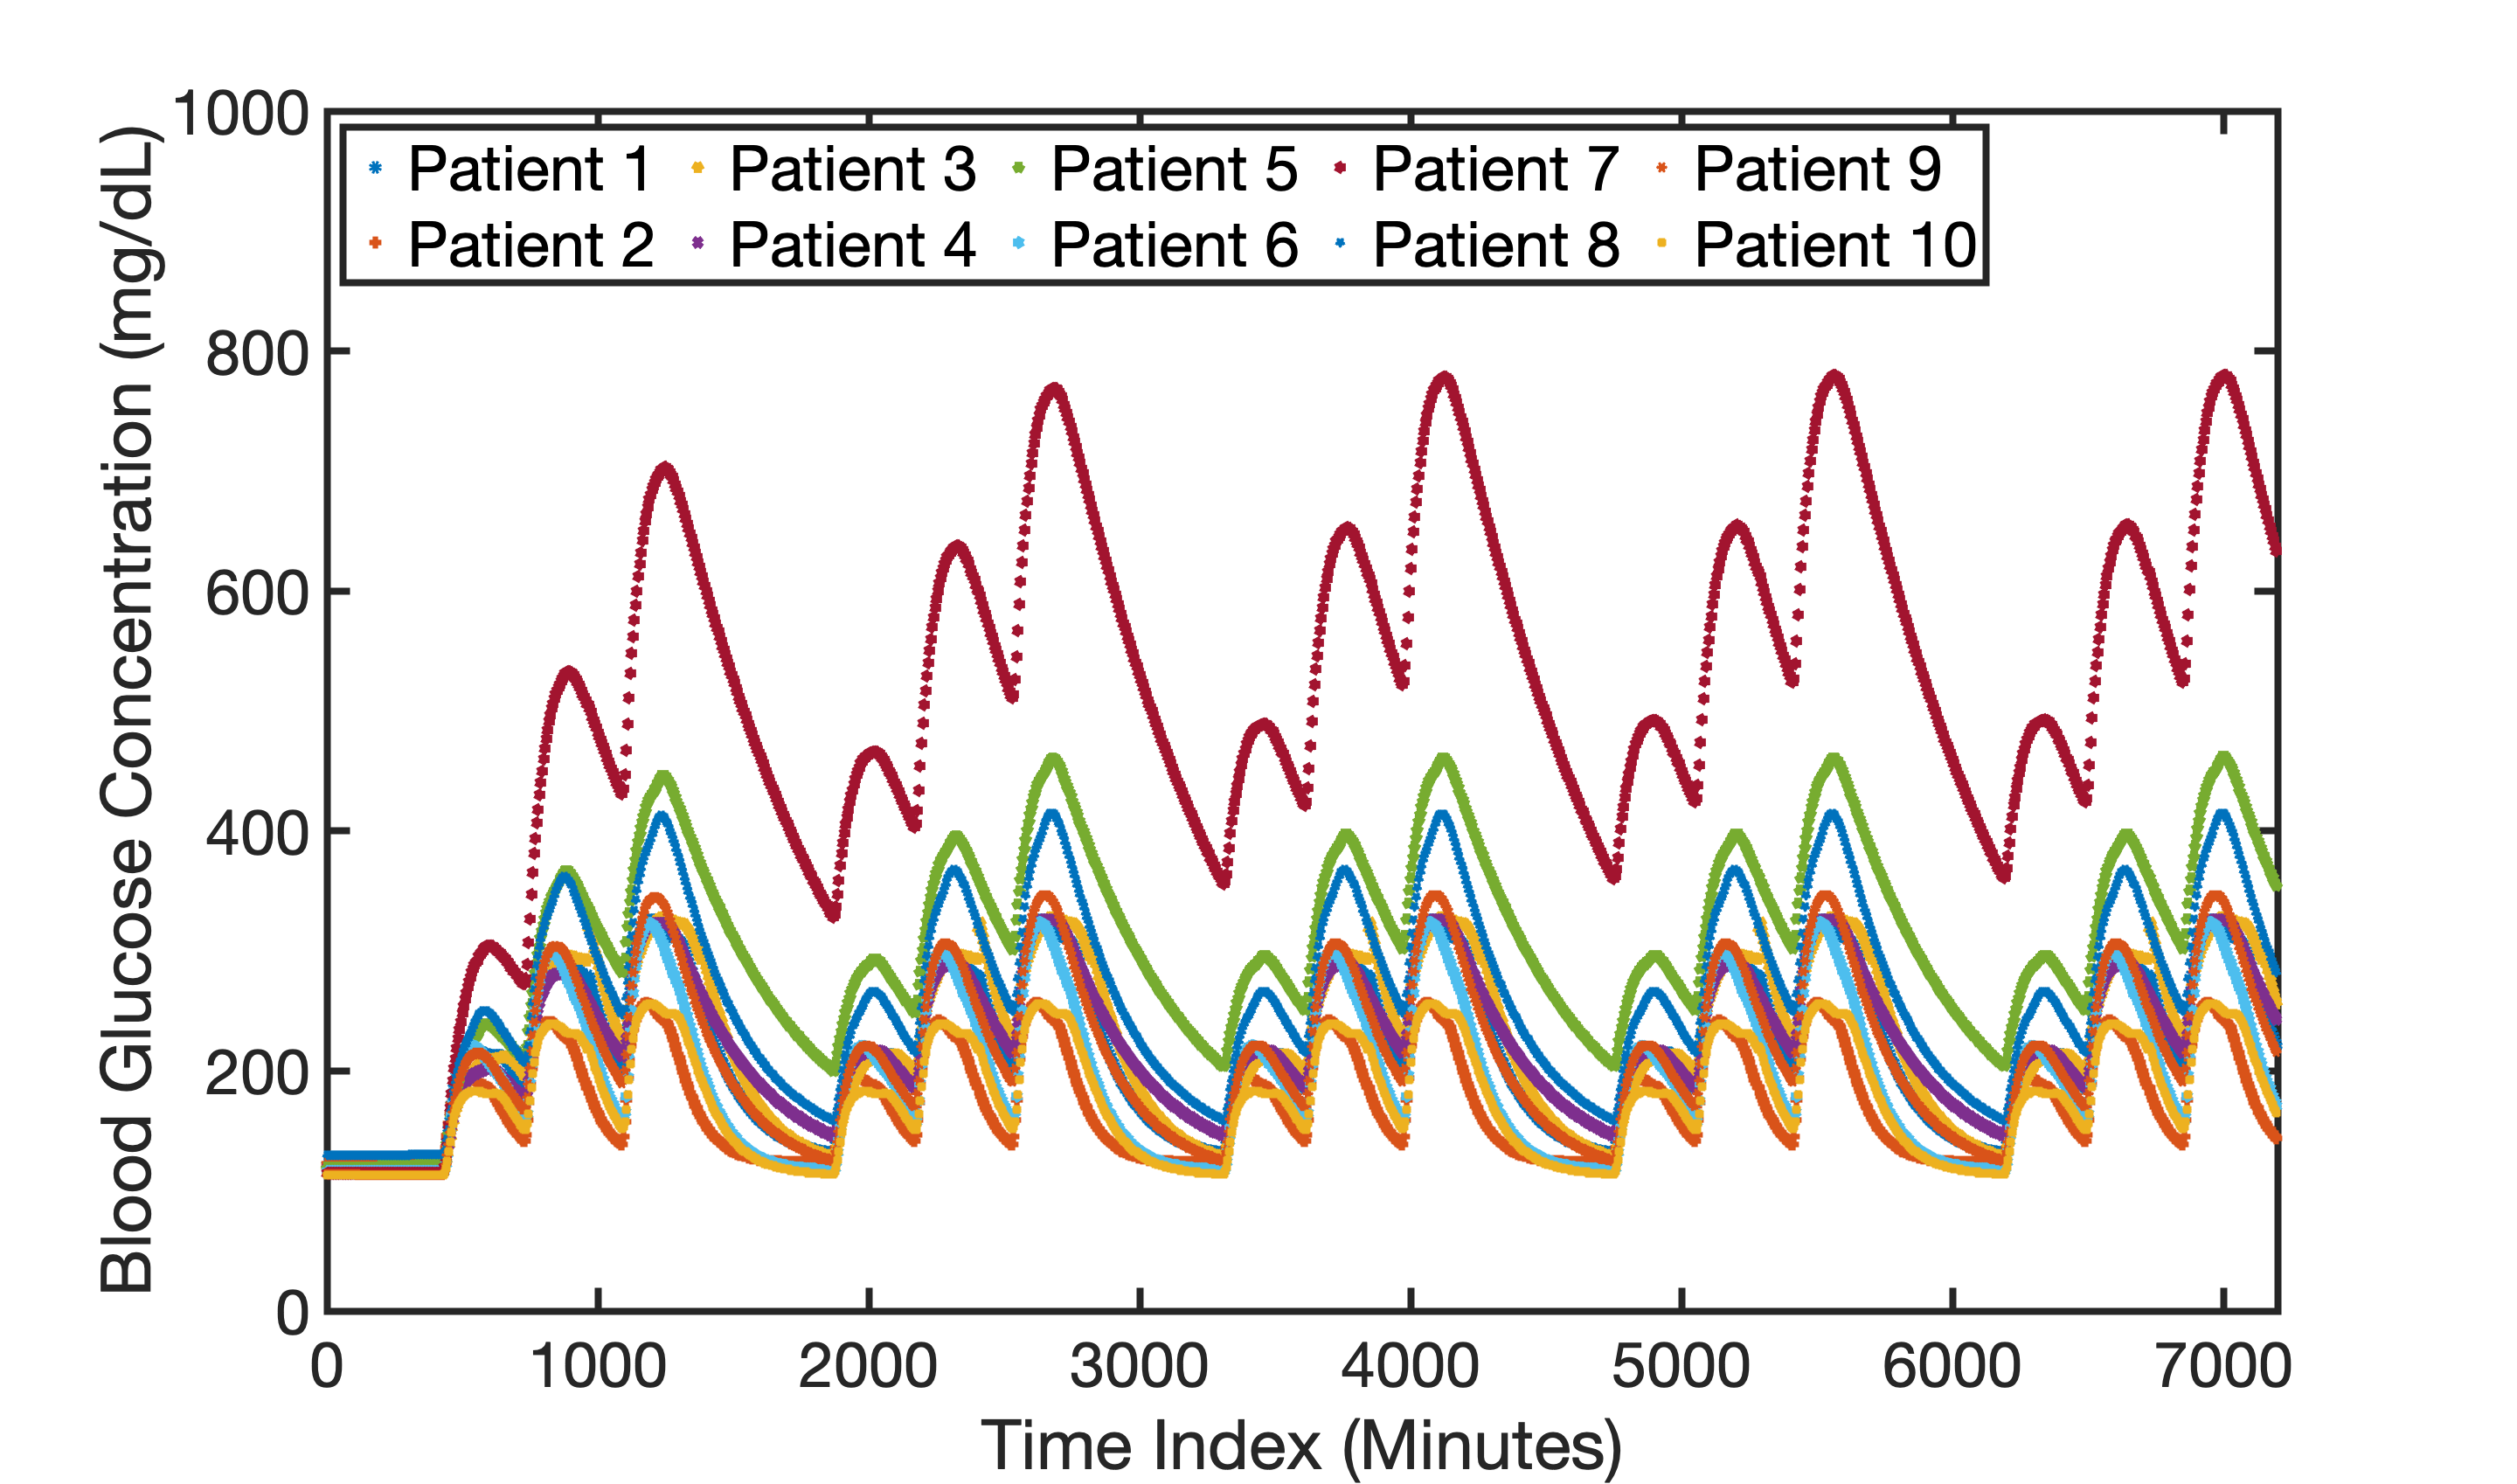
\includegraphics[width=0.6\linewidth]{Figures_manuscript/fda_data.png}
\caption{Blood-glucose trajectories for 10 adult in silico subjects generated using the UVA/Padova T1D simulator \cite{man2014uva}.}
\label{fig:uva}
\end{figure}

\begin{table}[H]
\footnotesize
\centering
\caption{Patient-wise 5-fold cross-validation splits for the 10 adult in silico patients.}
\label{tab:cv_folds}
\begin{tabular}{c l l}
\hline
\textbf{Fold} & \textbf{Training} & \textbf{Held out validation} \\
\hline
1 & Patients [1--8] & Patients [9, 10] \\
2 & Patients [1--5, 8--10] & Patients [6, 7] \\
3 & Patients [3--10] & Patients [1, 2] \\
4 & Patients [1, 2, 5--10] & Patients [3, 4] \\
5 & Patients [1--4, 6, 7, 9, 10] & Patients [5, 8] \\
\hline
\end{tabular}
\end{table}

%-- architecture pool
\paragraph{Candidate architecture pool}
The candidate TCN pool is constructed from the feasible architecture space in \eqref{eq:feasible_space}. To ensure adequate temporal context for glucose dynamics, architectures are constrained to satisfy
$
1~\text{day} \le \mathrm{RF}(\xi) \le 2000~\text{min},
$
where the lower bound ensures access to at least one daily cycle and the upper bound avoids unnecessarily long temporal context. We also enforce the no-holes condition \(f\geq b\) for dilated convolutions. Additional implementation bounds on filter size, depth, and channel width are imposed to keep the search computationally tractable. These constraints yield a finite pool of 61 candidate TCN architectures. For EVIDENT, the candidates are partitioned into six ordered capacity levels according to the number of trainable parameters, as summarized in Table~\ref{tab:arch_level}. Full architecture specifications are provided in ~\ref{app:architecture_pool}.

%-- training specifics/validation protocol
\paragraph{Validation protocol}
The training and validation protocol is designed to emulate deployment to unseen T1D subjects with limited subject-specific data. In each cross-validation fold, candidate architectures are first trained on population data using input--output windows extracted from inter-meal intervals. The output horizon is set to 285 minutes, corresponding to the minimum inter-meal gap, and windows containing meal events within the prediction horizon are excluded.
%
For each held-out subject, the posterior distribution obtained from population training is subsequently used as the prior for subject-specific adaptation using four days of that subject’s data. Validation is then performed using rolling one-hour prediction windows  shifted to cover the full day 5, while excluding windows intersecting meal events and truncating predictions 10 minutes before meal onset to avoid scoring across unobserved disturbances. A candidate architecture is considered acceptable if its NLPD remains below the prescribed tolerance \(Tol=14.5\) across all one-hour validation windows for both held-out subjects.

\begin{footnotesize}
\setlength{\tabcolsep}{5pt}
\renewcommand{\arraystretch}{1.3}
\begin{longtable}{p{1.8cm}p{1.8cm}p{2.0cm}p{2.0cm}p{1.6cm}p{1.8cm}p{2.0cm}}
\caption{Candidate TCN architectures organized into six capacity levels based on the number of trainable parameters. Each row reports the range of architecture hyperparameters used in level $l$: the number of temporal blocks $N$, filter size $f$, dilation base $b$, and starting number of encoder channels $c_1$. The dilation factor in encoder block $j$ is defined as $\delta_j = b^{j-1}$, and the number of encoder channels follows a doubling schedule $c_j = 2^{j-1} c_1$ for $j = 1, \dots, N$. The decoder channels $\{\tilde{c}_j\}_{j=1}^{N}$ mirrors the encoder channels in reverse order.}
\label{tab:arch_level}\\
\toprule
\textbf{Capacity level $l$} & \textbf{Parameter range} & \textbf{Number of architectures} & \textbf{Number of temporal blocks $N$} & \textbf{Filter size $f$} & \textbf{Dilation base $b$} & \textbf{Starting number of channels $c_1$} \\
\midrule
\endfirsthead
\toprule
\textbf{Capacity level $l$} & \textbf{Parameter range} & \textbf{Number of architectures} & \textbf{Number of temporal blocks $N$} & \textbf{Filter size $f$} & \textbf{Dilation base $b$} & \textbf{Starting number of channels $c_1$} \\
\midrule
\endhead
\endfoot
\bottomrule
\endlastfoot
1 & $\le 30$k      & 10 & $[3-4]$          & $[7- 13]$ & $[4- 9]$ & $[2, 4]$     \\
2 & $30$k--$100$k  &  9 & $[3- 6]$    & $[3- 13]$ & $[3- 9]$ & $[2, 8]$     \\
3 & $100$k--$400$k & 10 & $[3- 6]$    & $[3- 13]$ & $[2- 9]$ & $[2, 16]$    \\
4 & $400$k--$1$M   & 11 & $[3- 7]$ & $[3- 13]$ & $[2- 9]$ & $[2, 32]$    \\
5 & $1$M--$5$M     & 11 & $[3- 7]$ & $[3- 13]$ & $[2- 9]$ & $[4, 64]$    \\
6 & $\ge 5$M       & 10 & $[3- 7]$ & $[7- 13]$ & $[2-9]$ & $[8, 128]$   \\
\end{longtable}
\end{footnotesize}




%++++++++++++++++++++++++++++++++++++++++++++++++++++++++++++++++++++++++
\subsubsection{Level-wise architecture discovery results}

\paragraph{Capacity Level 1 ($l=1$)}
The lowest-capacity TCN candidates with less than $3 \times 10^4$ parameters, that still satisfy the receptive-field feasibility constraints, are in Level~1.
As shown in Figure \ref{fig:level1_plausibility_predict}, model evidence is not uniformly distributed within this level and it concentrates on a small subset of architectures in each held-out validation fold. 
Despite this, none of the Level~1 architectures satisfy the validation criterion. As illustrated in Figure~\ref{fig:level1_plausibility_predict}, predictions on held-out subjects frequently violate the NLPD tolerance across one-hour windows (shown in red). These failures indicate that, although some architectures are favored by the population-based training data, their representational capacity is insufficient to generalize to subject-specific glucose dynamics. Consequently, EVIDENT rejects Level~1 and proceeds to the next capacity level.


\begin{figure}[!ht]
\centering
%--- plausibility (Level 1)
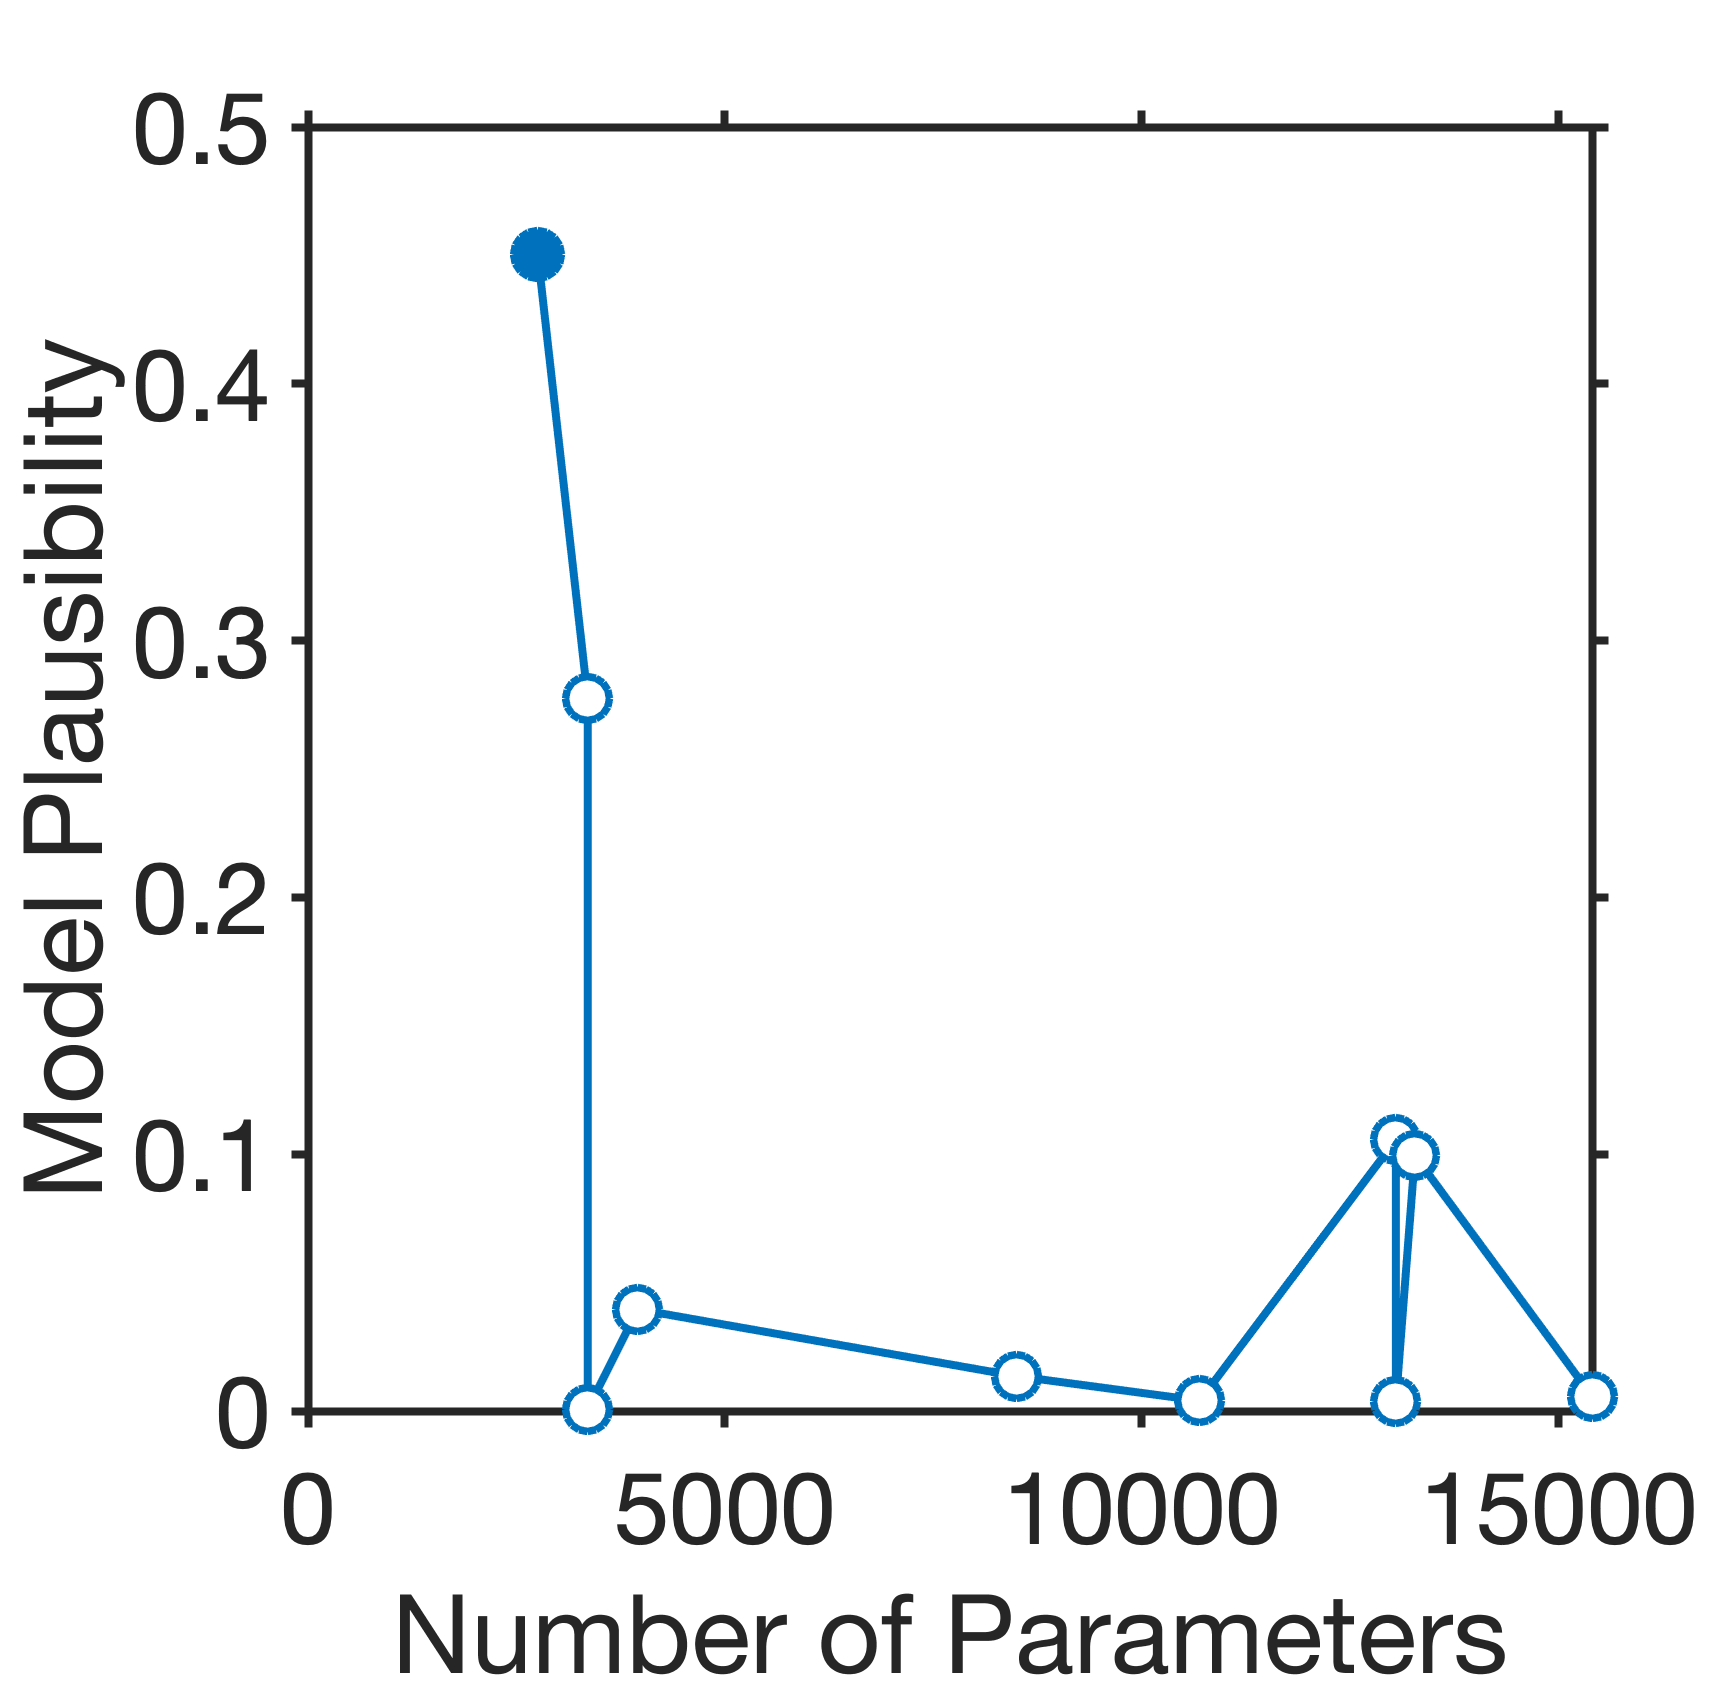
\includegraphics[width=0.19\textwidth]{Figures_manuscript/cat1_fold1.png}\hfill
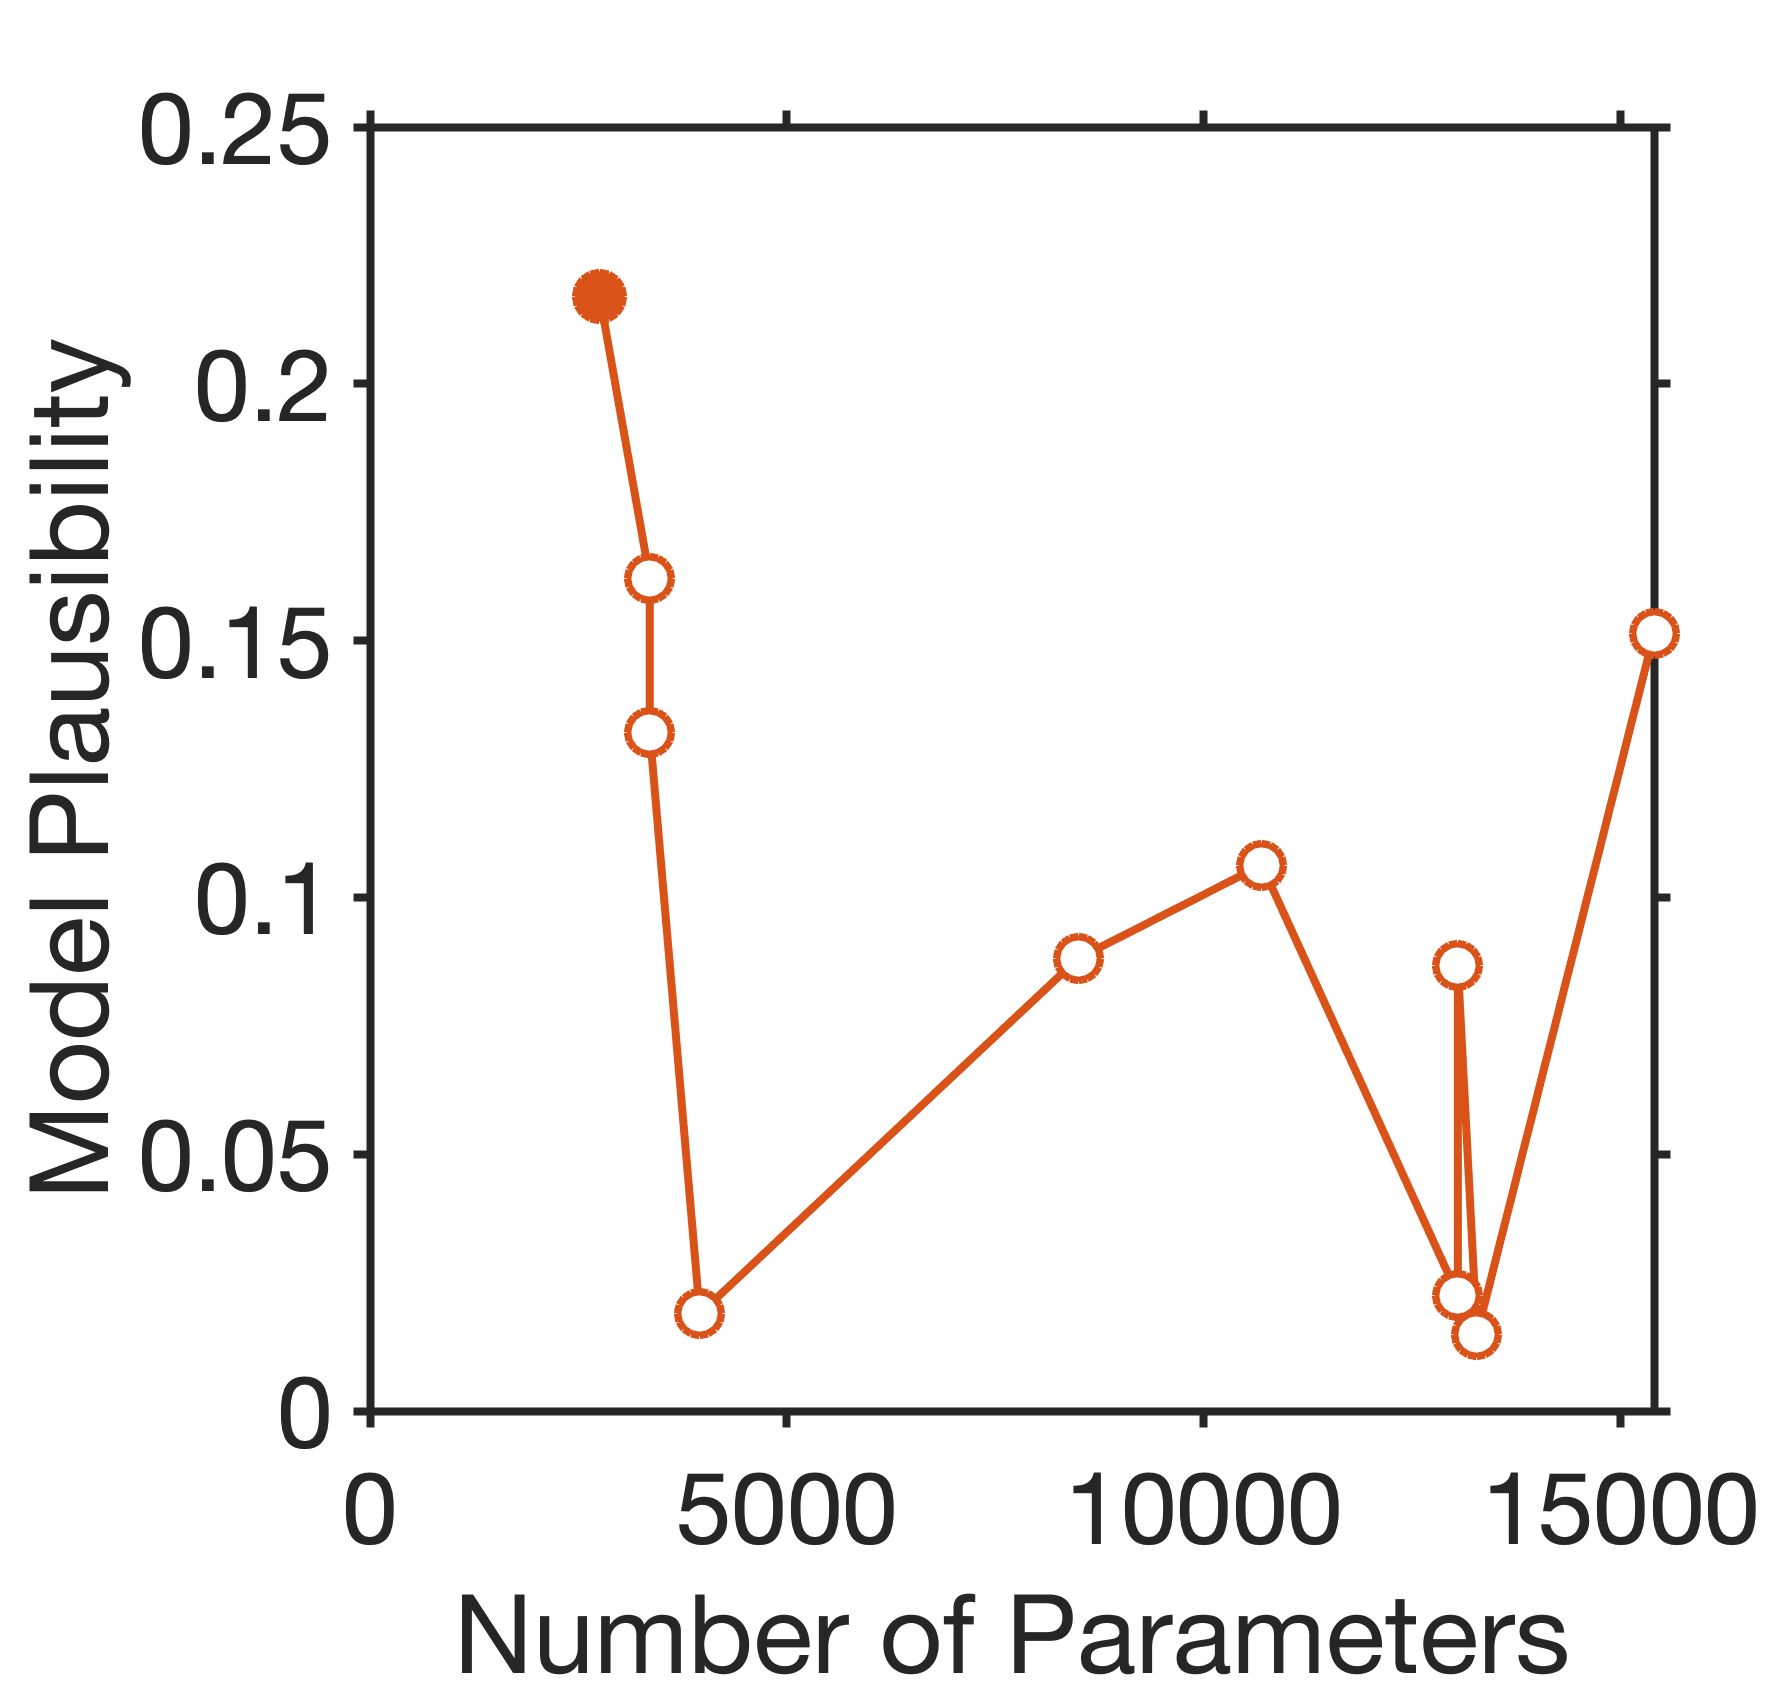
\includegraphics[width=0.19\textwidth]{Figures_manuscript/cat1_fold2.png}\hfill
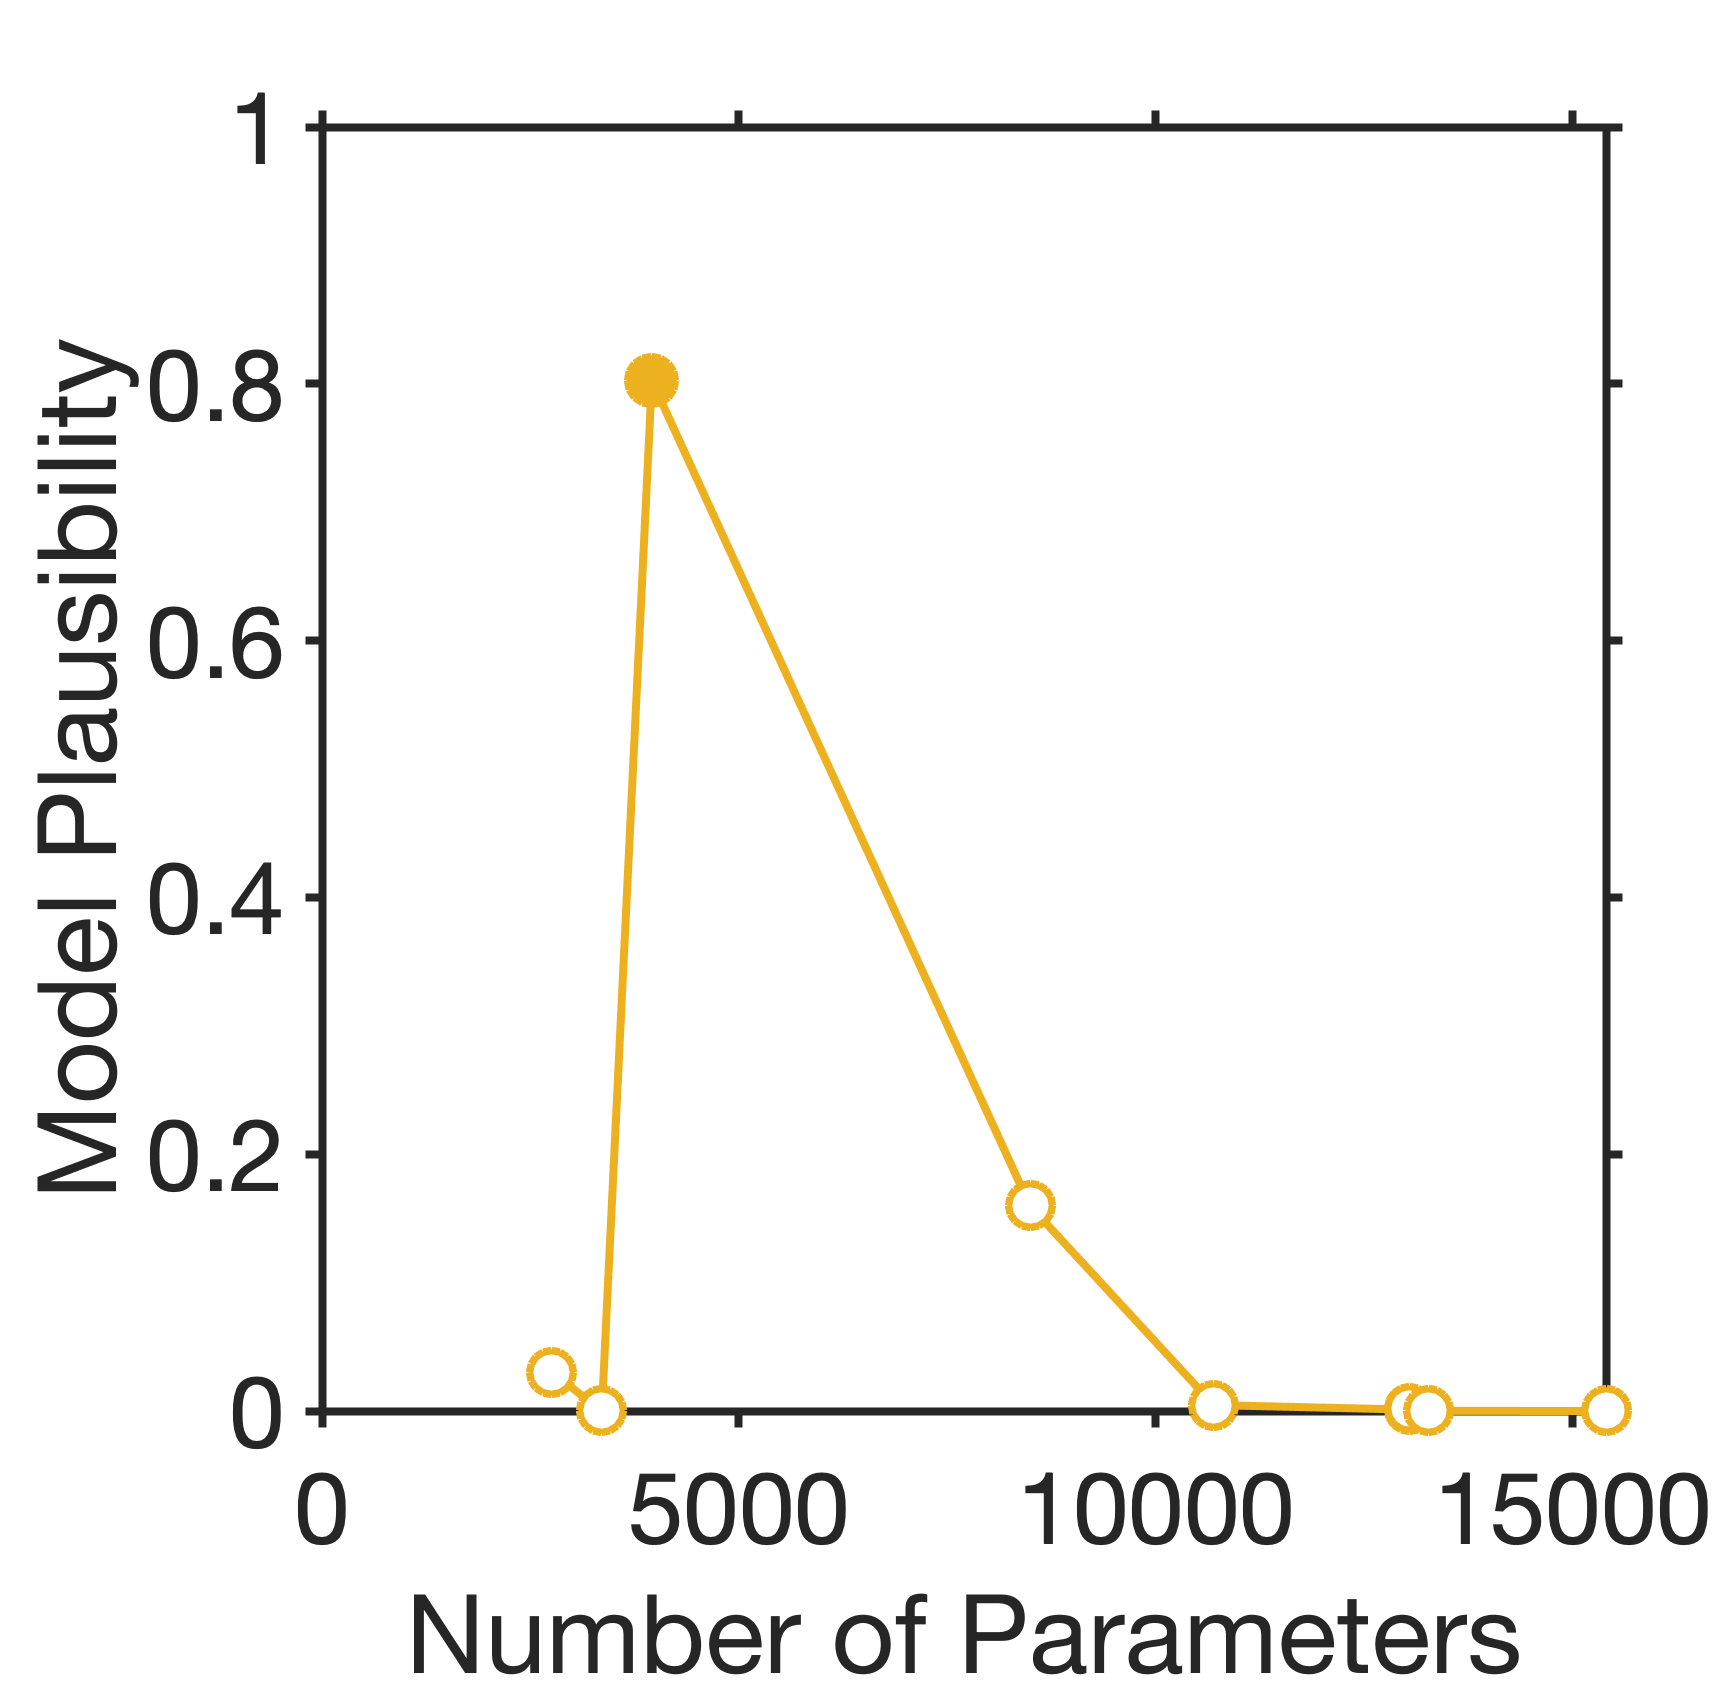
\includegraphics[width=0.19\textwidth]{Figures_manuscript/cat1_fold3.png}\hfill
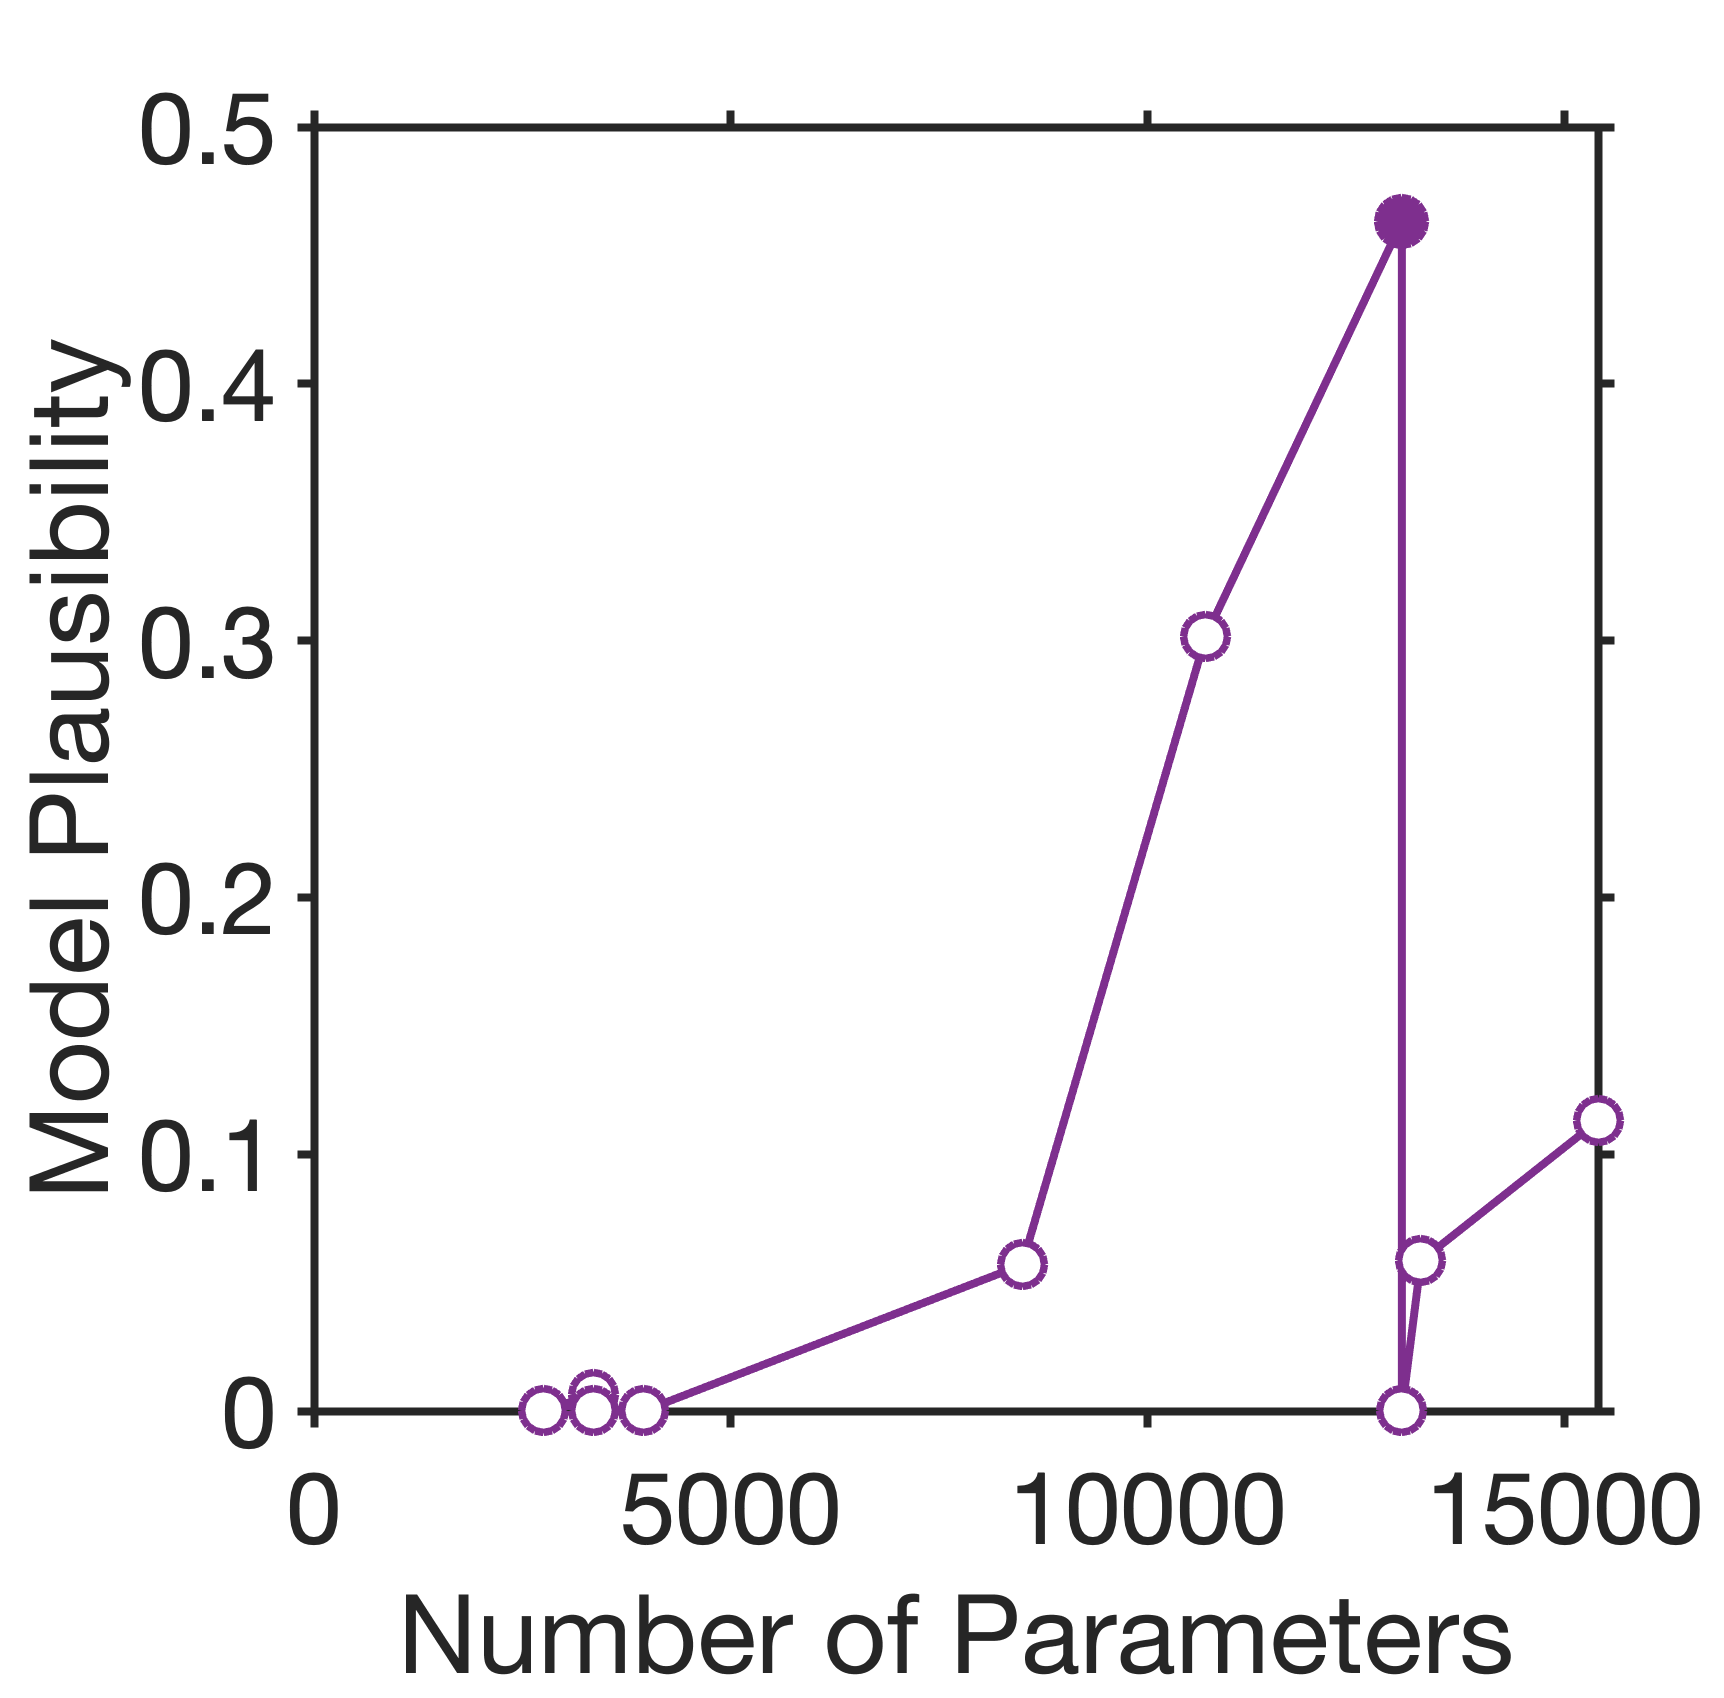
\includegraphics[width=0.19\textwidth]{Figures_manuscript/cat1_fold4.png}\hfill
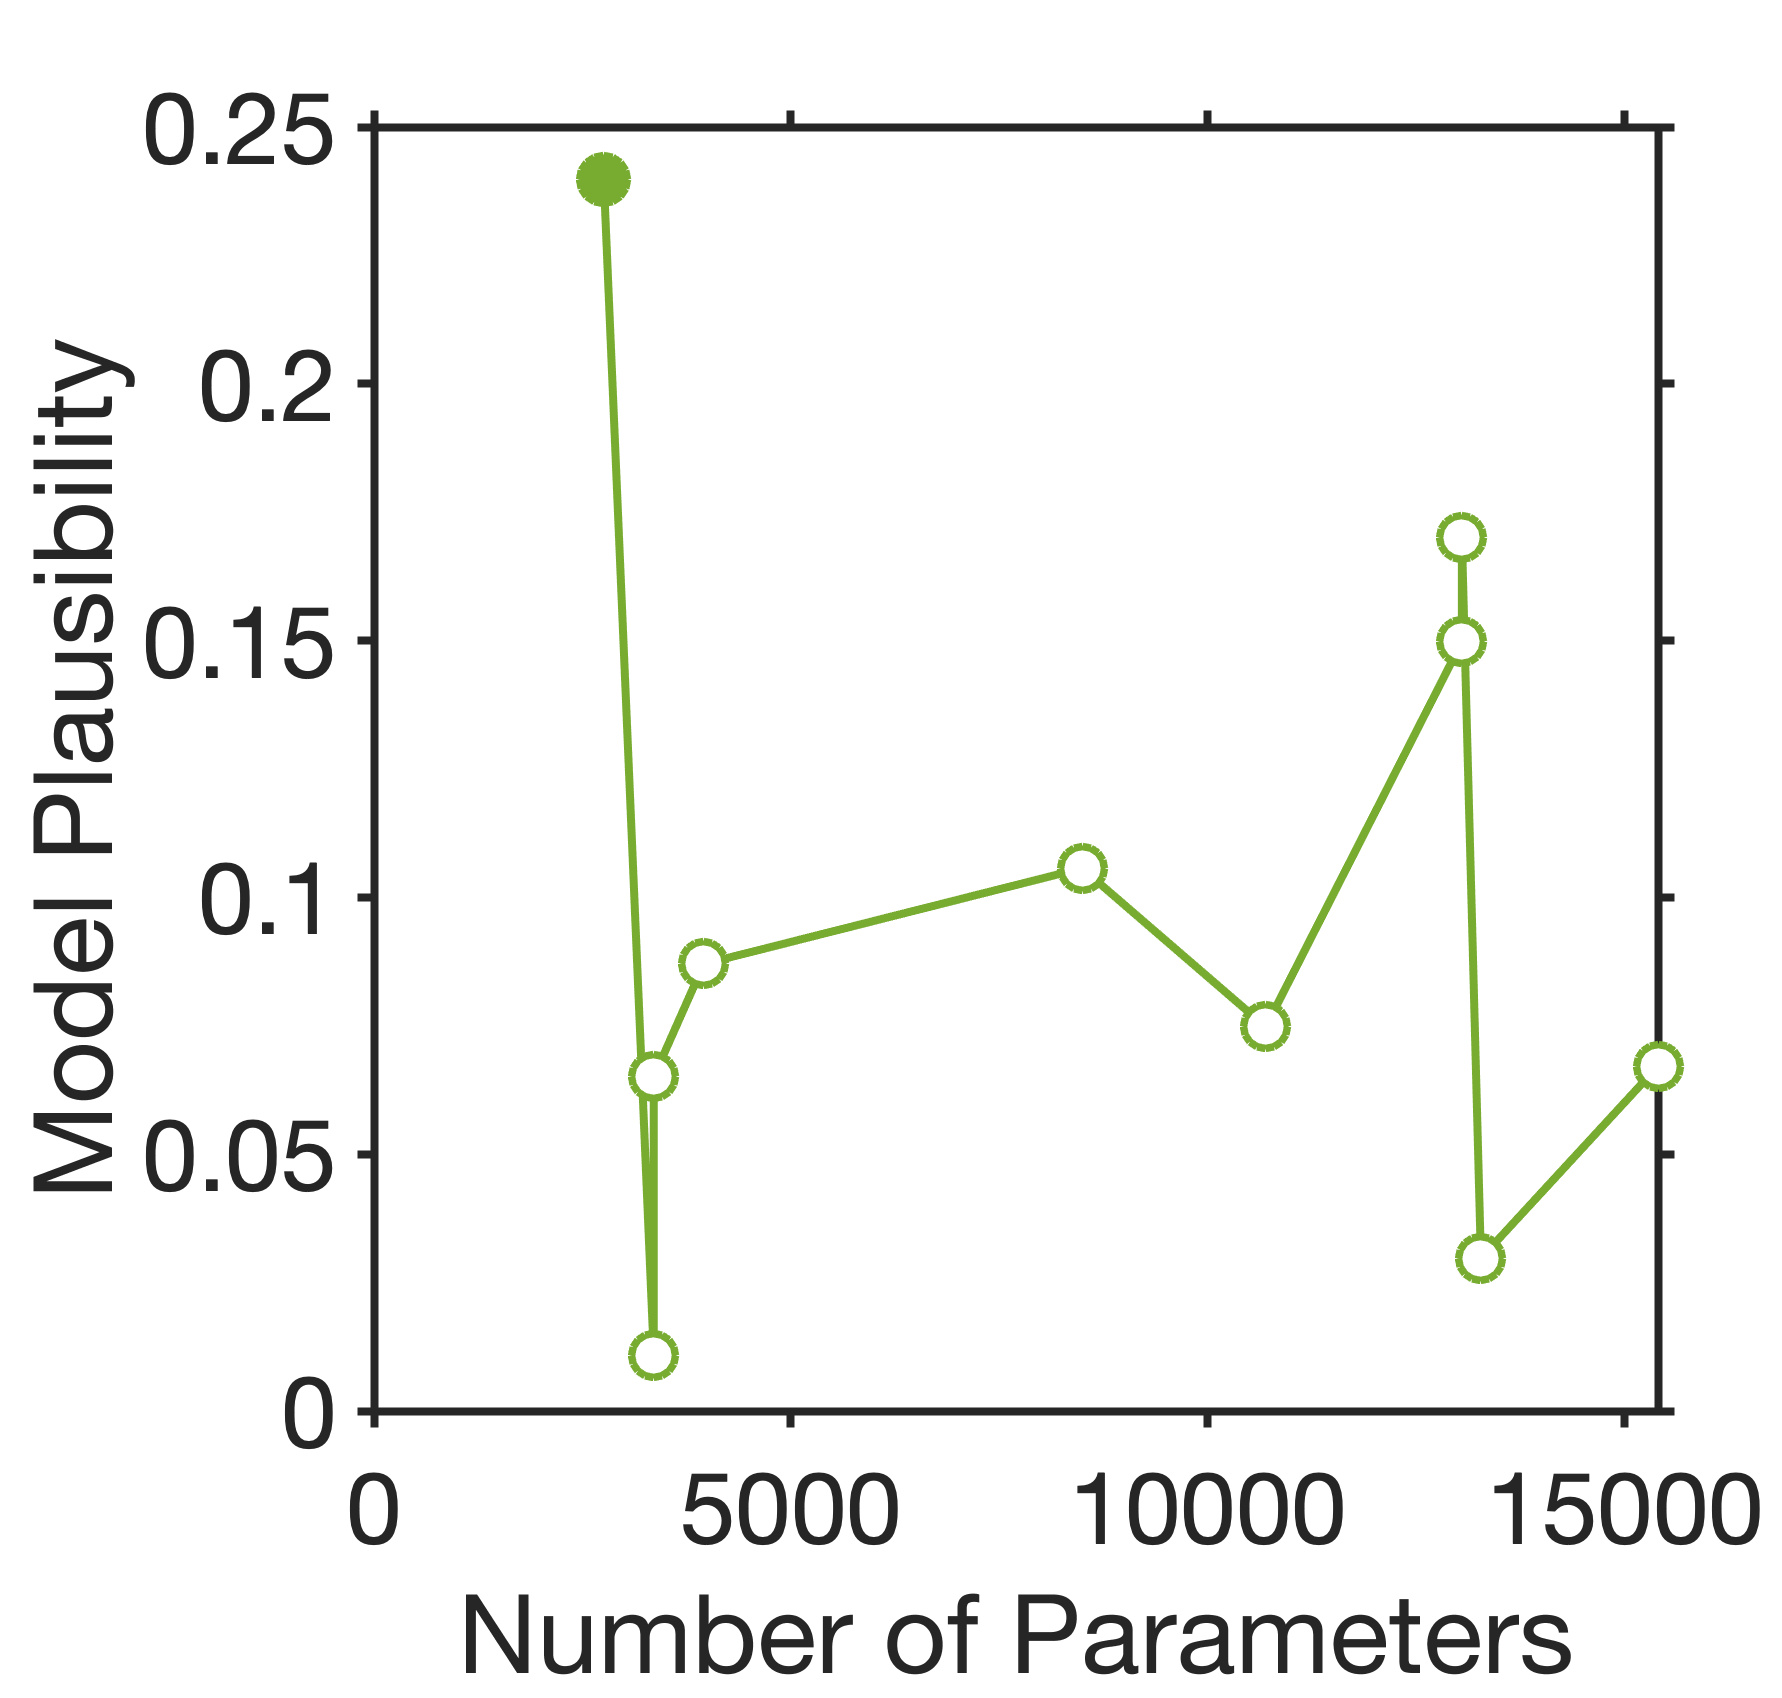
\includegraphics[width=0.19\textwidth]{Figures_manuscript/cat1_fold5.png}
\\(a)\\
%--- BG prediction - fale
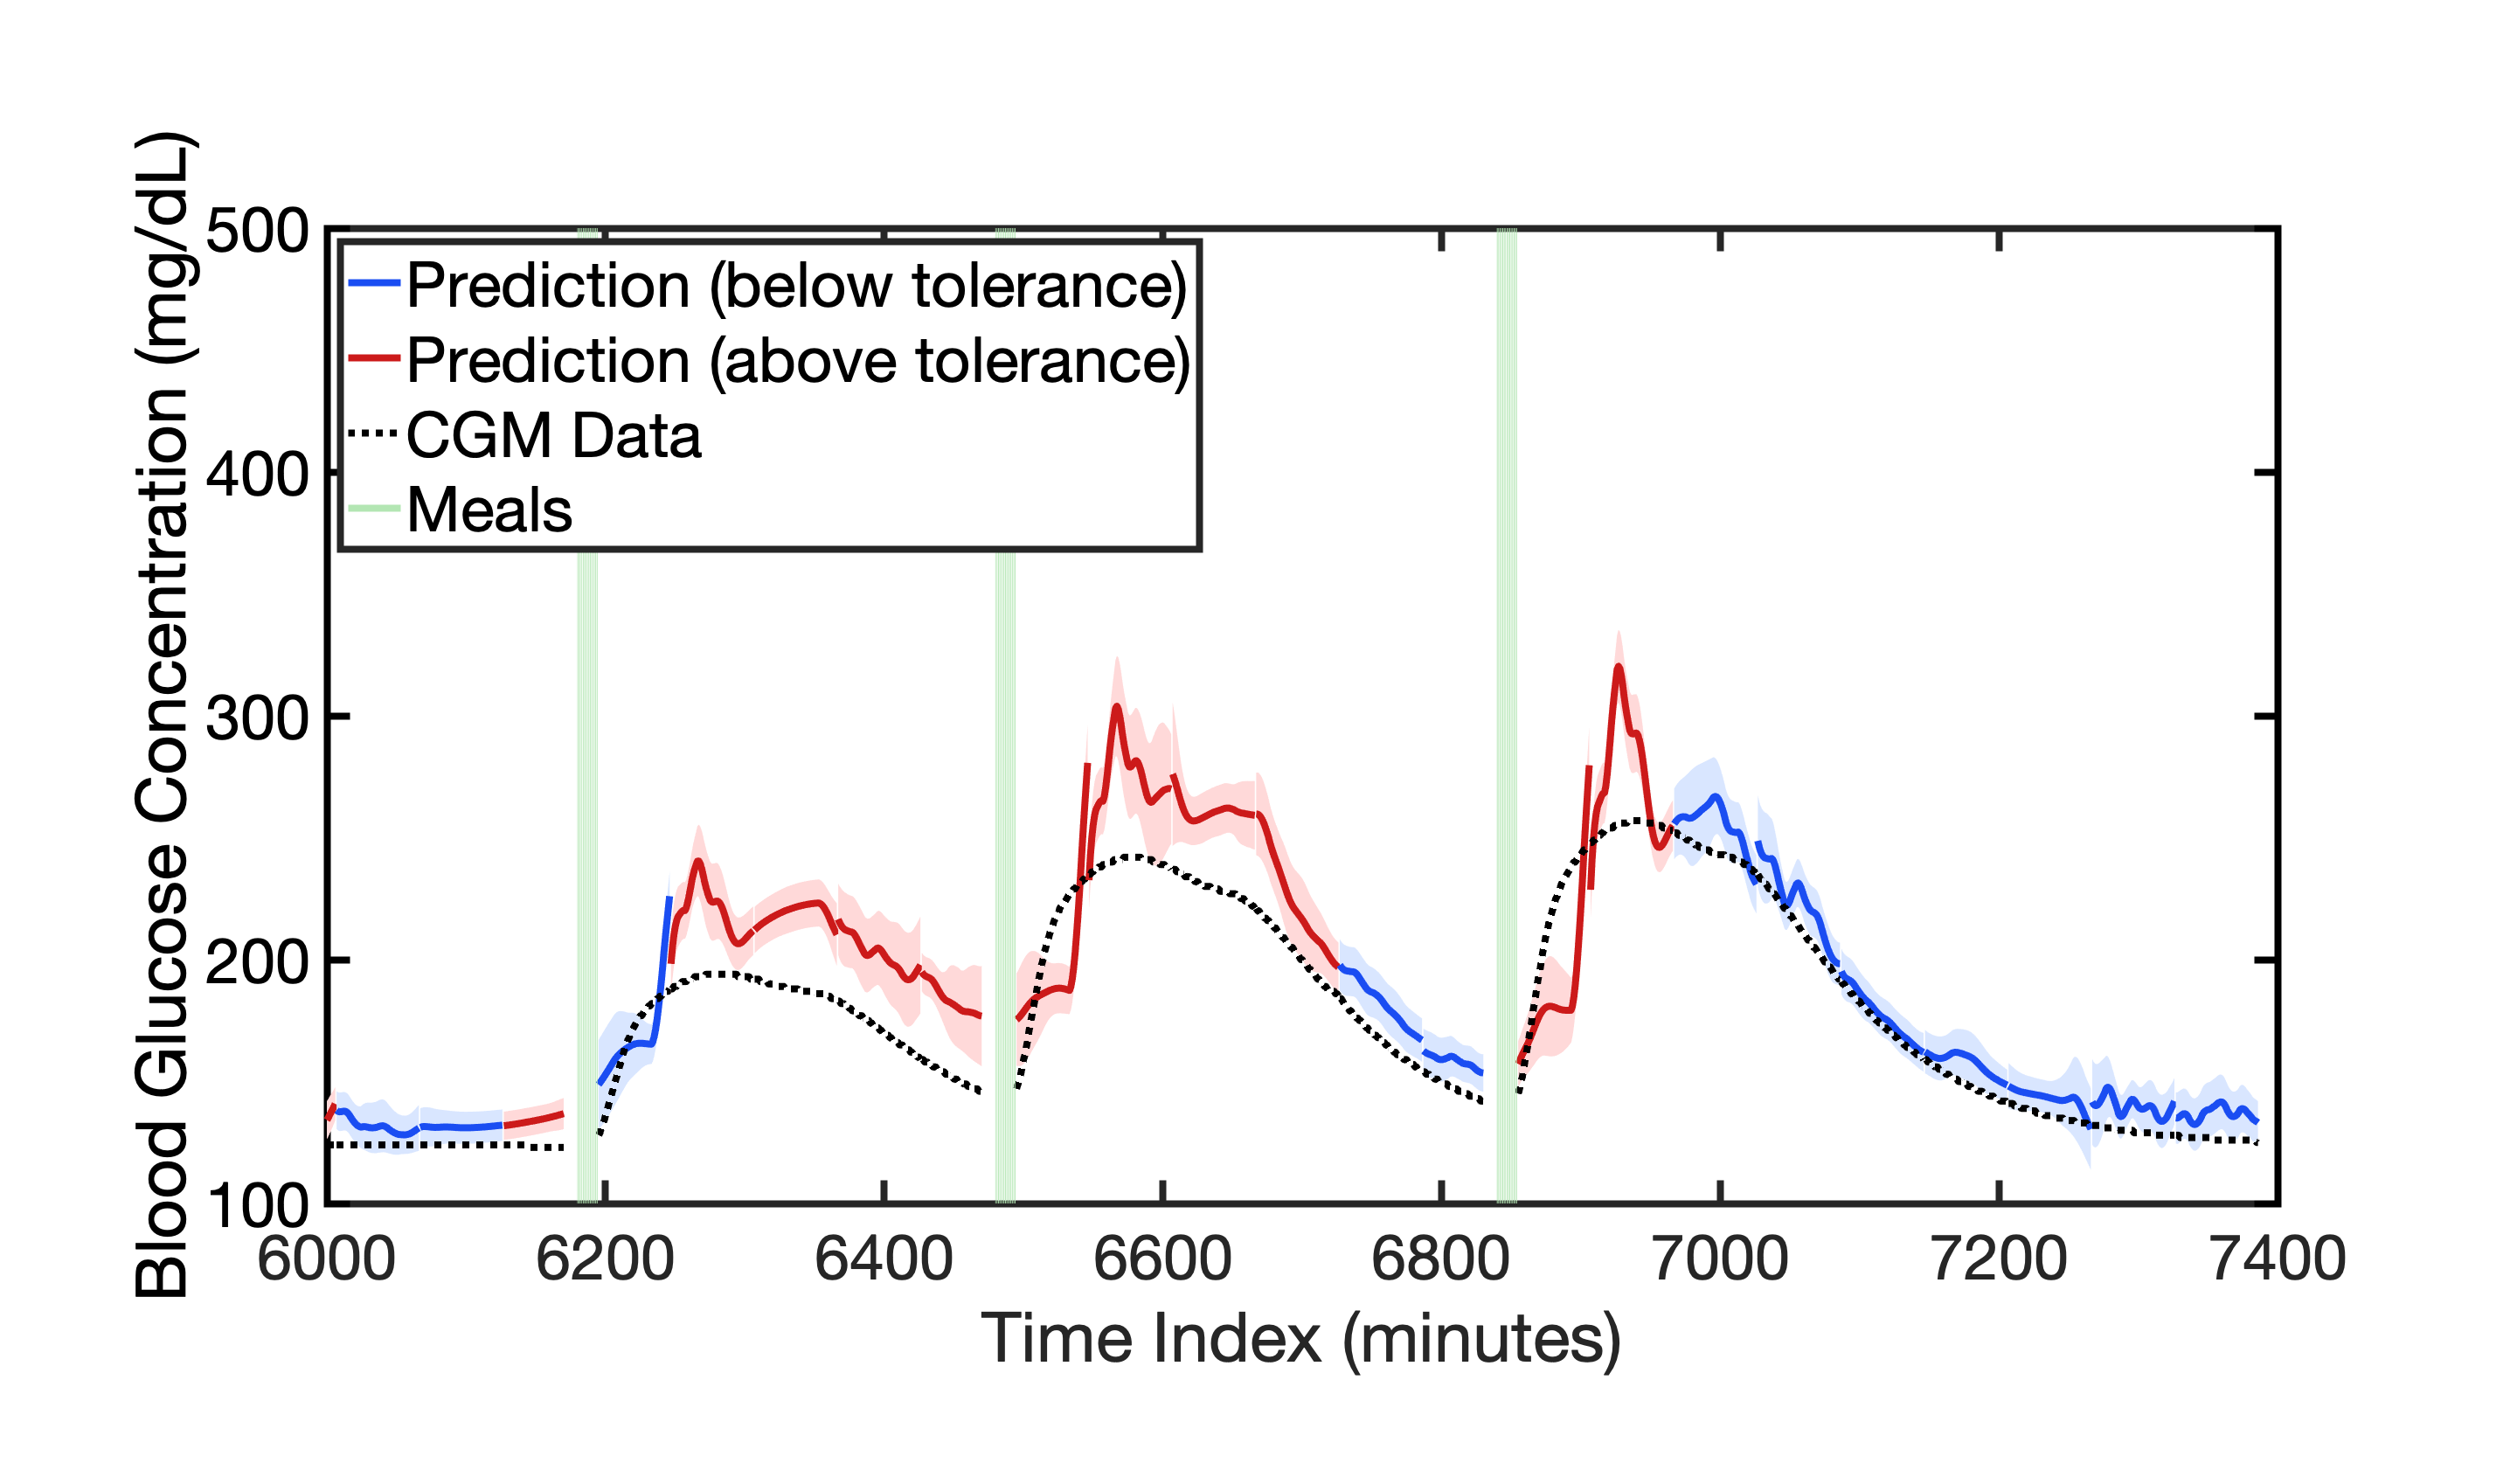
\includegraphics[width=0.45\linewidth]{Figures_manuscript/cat1_p2_c1.png}
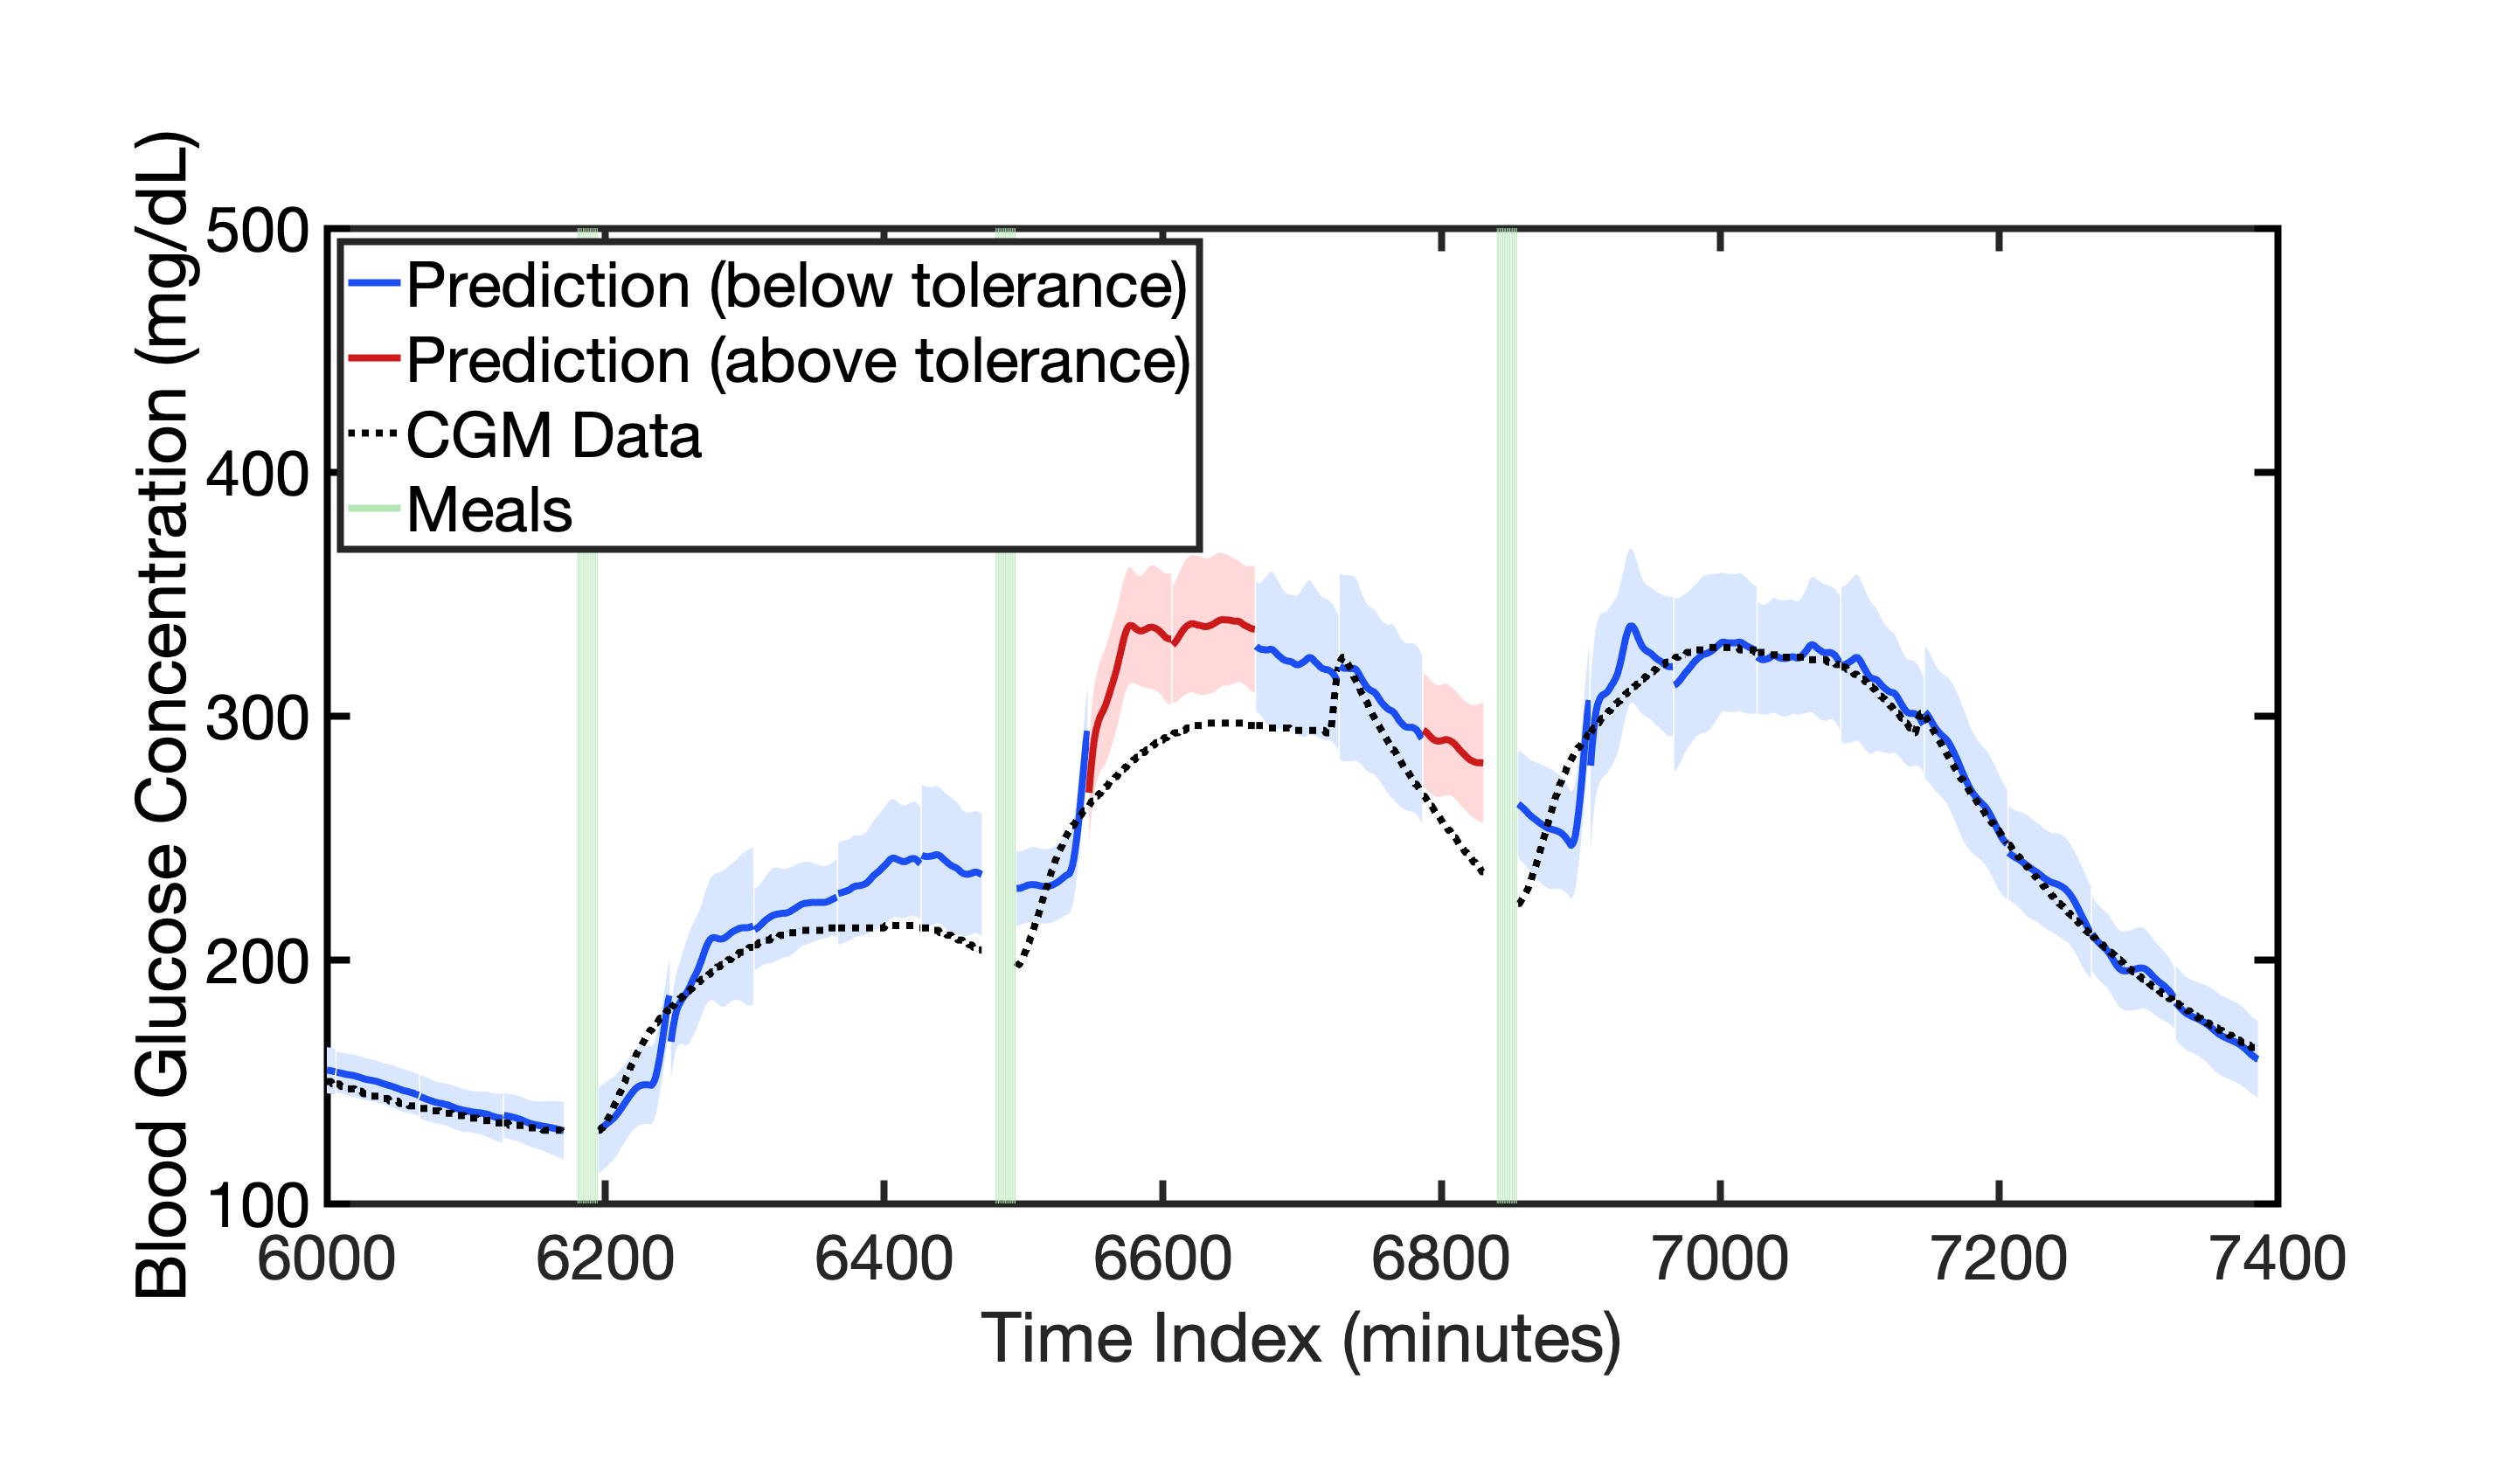
\includegraphics[width=0.45\linewidth]{Figures_manuscript/cat1_p3_c1.png}
\\(b) \hspace{2.5in} (c)\\
\caption{
Level~1 architecture ranking and validation outcome. 
(a) Posterior plausibility \(\rho\) versus model size (number of parameters) for Level~1 architectures across validation folds (left to right: folds 1–5). 
(b,c) Representative validation failure for most plausible architectures on held-out subjects: (b) Patient 2 from fold 3, Architecture: $Level_1Arch_4$, (c) Patient 3 from fold 4, Architecture: $Level_1Arch_6$.
Red segments indicate one-hour prediction windows that violates the acceptance criterion $NLPD \leq Tol$.
}
\label{fig:level1_plausibility_predict}
\end{figure}





\paragraph{Capacity Level~2 ($l=2$)}
Level~2 contains the intermediate-capacity regime ($3\times10^4 - 1\times10^5$ parameters) in which EVIDENT identifies architectures that are both plausible and validation-acceptable. 
%-- Level 2: plausibility/sigma-noise
Figure \ref{fig:level2_plausibility_failure_sucess}(a) summarizes, for each held-out validation fold, the variation of posterior plausibility $\rho$ and the corresponding MAP estimate of $\sigma_{\text{noise}}$ across the candidate architectures in this level. It is observed that a small subset of architectures receives substantial posterior model plausibility, while the most plausible architecture varies across folds, reflecting the inter-patient heterogeneity of the population-based training data in Figure \ref{fig:uva}. While most subjects exhibit comparable glucose ranges and excursion patterns, Patient 7 and Patient 5 display substantially larger amplitudes, which changes the temporal structure seen during training. As a result, EVIDENT favors different architectures across folds. Nevertheless, $Level_2Arch_4$ with 43268 parameters, which consists of 5 temporal blocks with dilation base $b=3$, filter size $f=9$, and encoder channels $[2,4,8,16,32]$, emerges as a competitive architecture in three validation folds. This architecture achieves a one-day receptive field through gradual dilation growth across depth, while retaining sufficient local temporal resolution to capture meal-driven glucose excursions.
The $\sigma_{{\rm noise}_{MAP}}$ trends provide a diagnostic such that low-plausibility architectures require inflated noise levels, indicating that unresolved temporal structure is absorbed as noise, whereas competitive models achieve high plausibility without such inflation.

% Level 2 plot -- plausibility, representative failur, sucess
\begin{figure}[H]
\centering
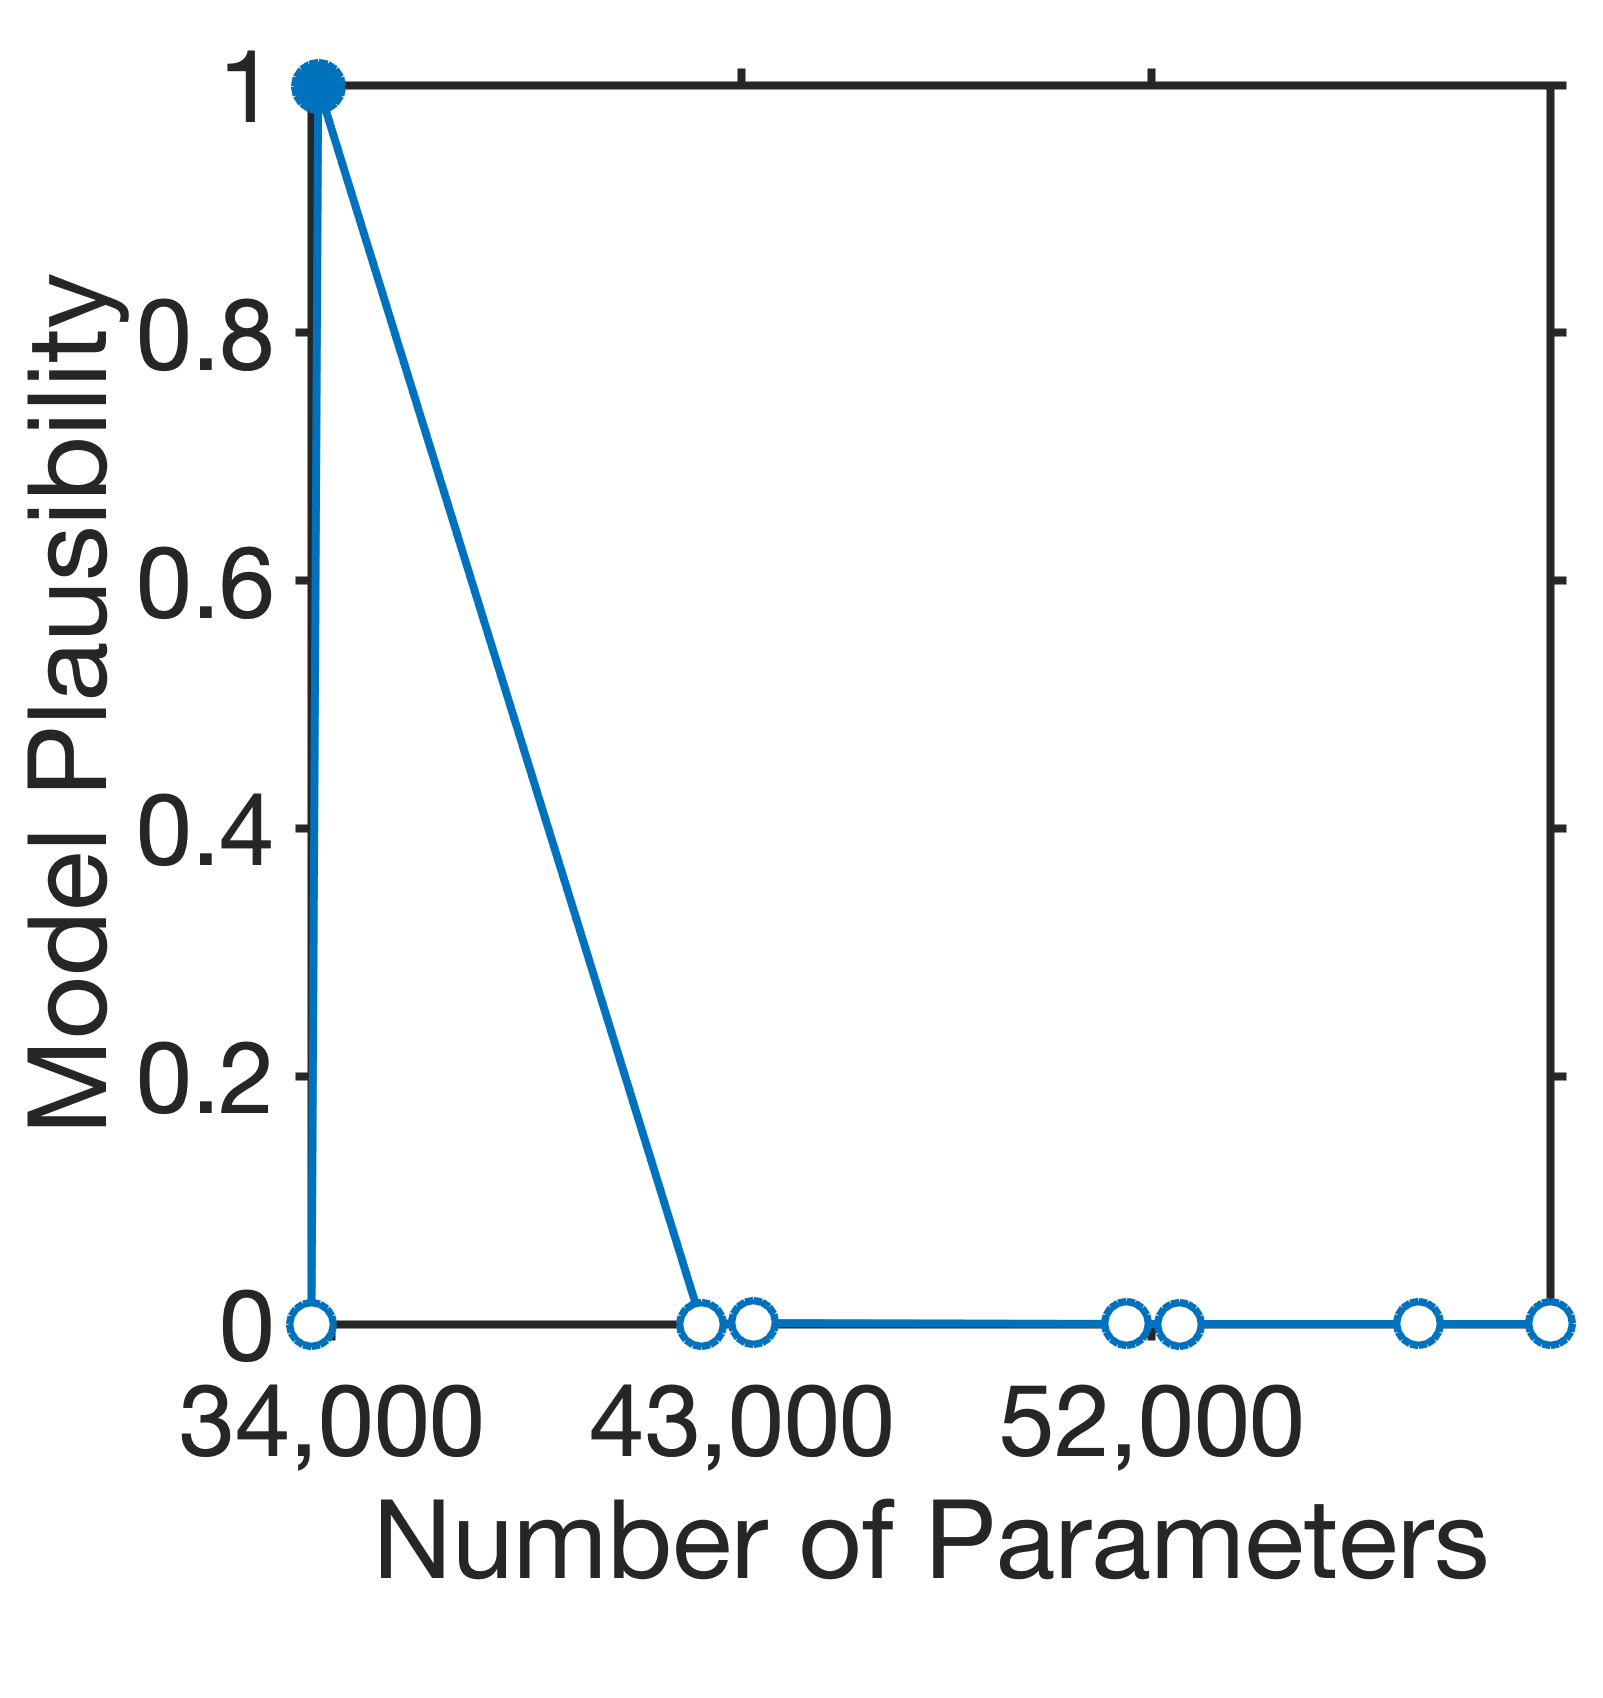
\includegraphics[width=0.19\textwidth]{Figures_manuscript/cat2_fold1.png}\hfill
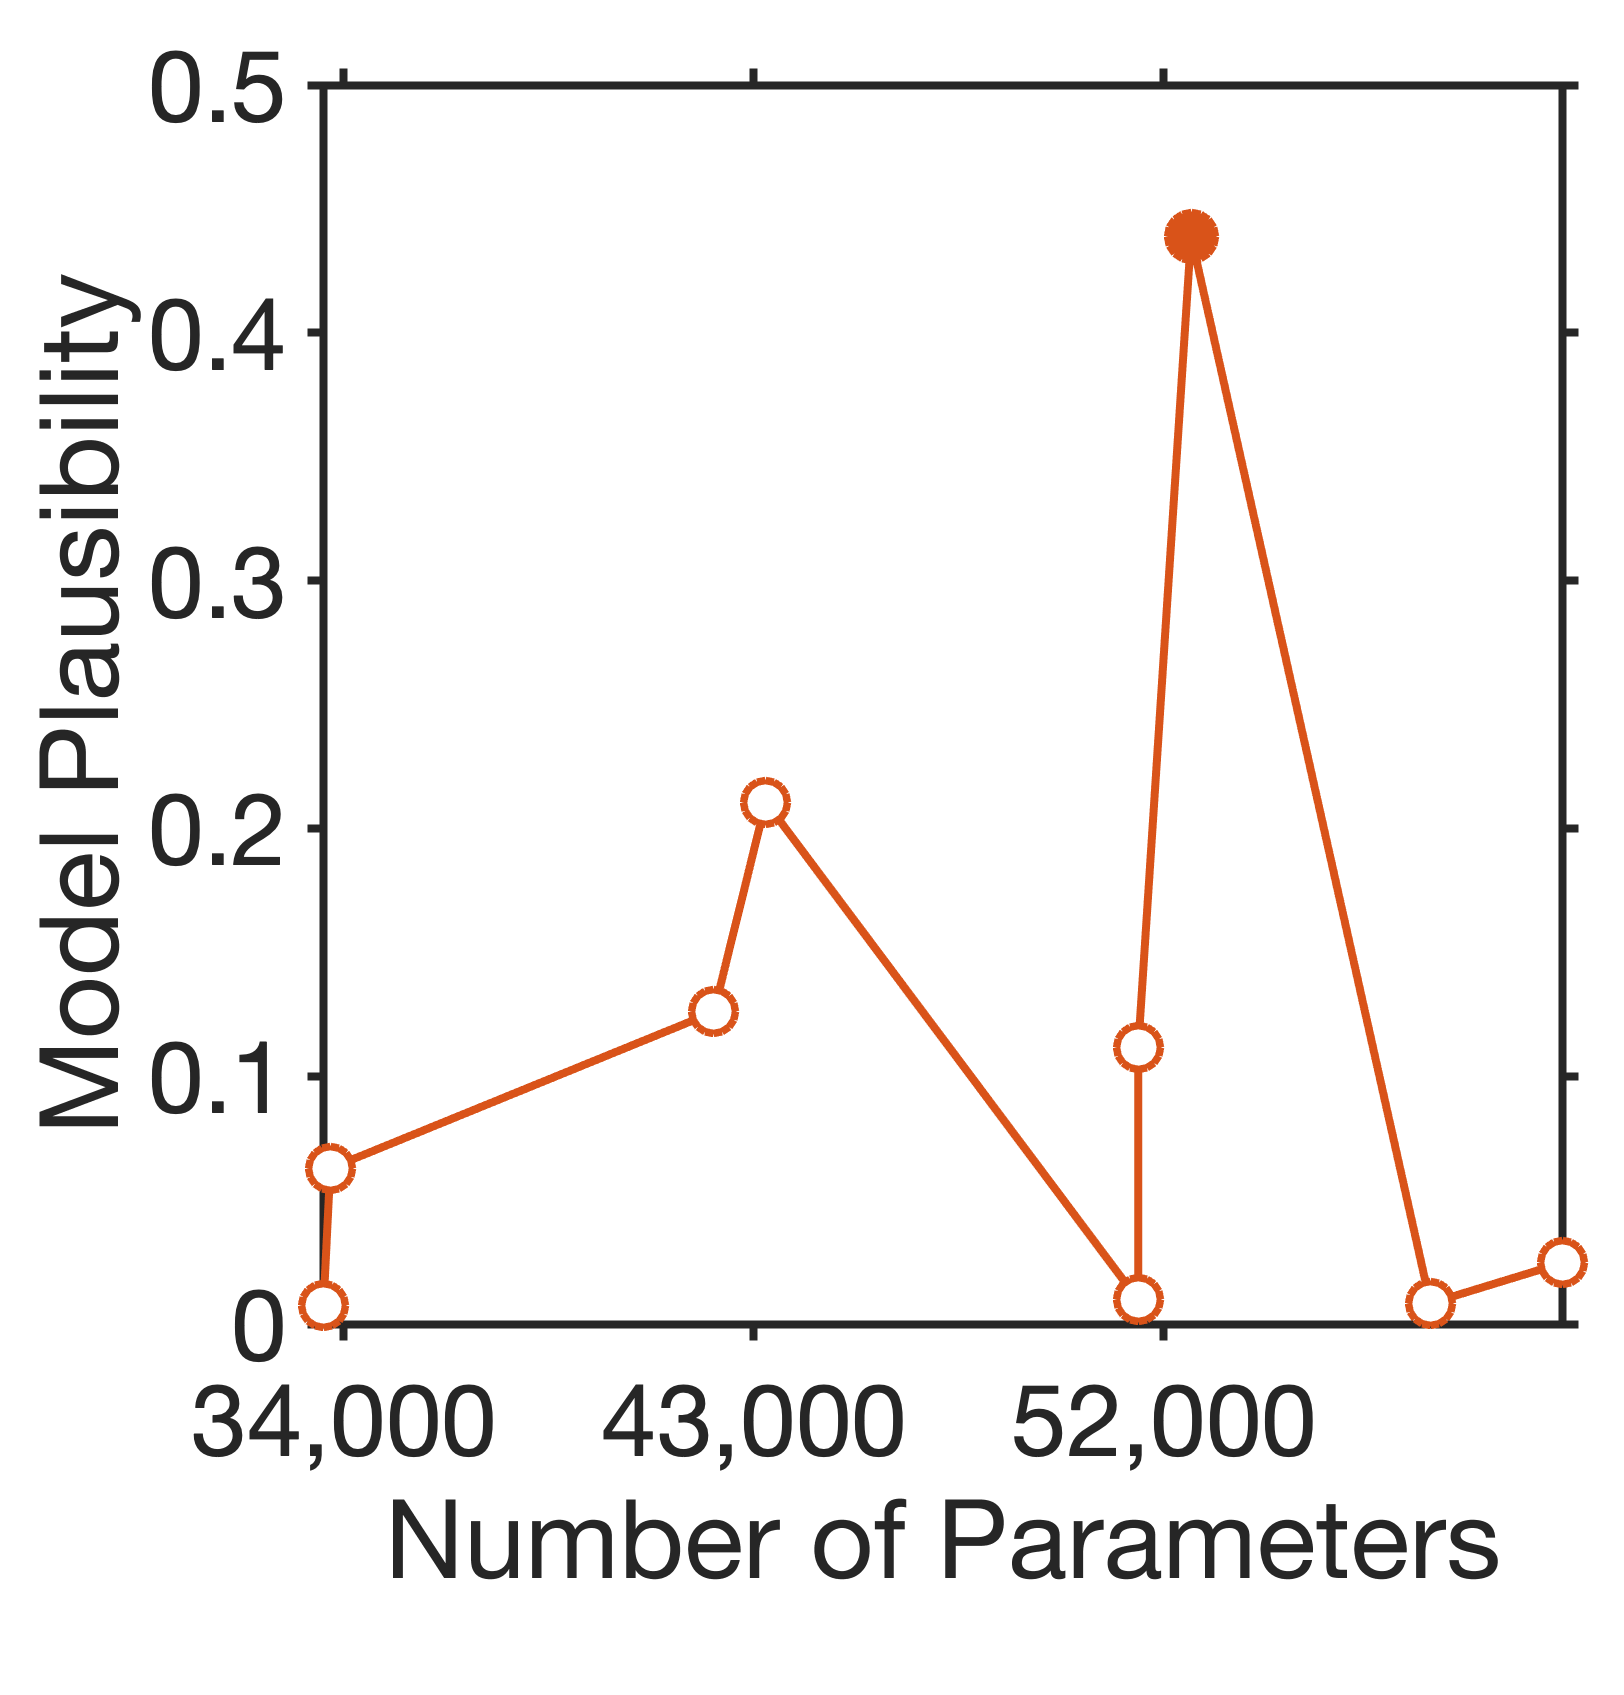
\includegraphics[width=0.19\textwidth]{Figures_manuscript/cat2_fold2.png}\hfill
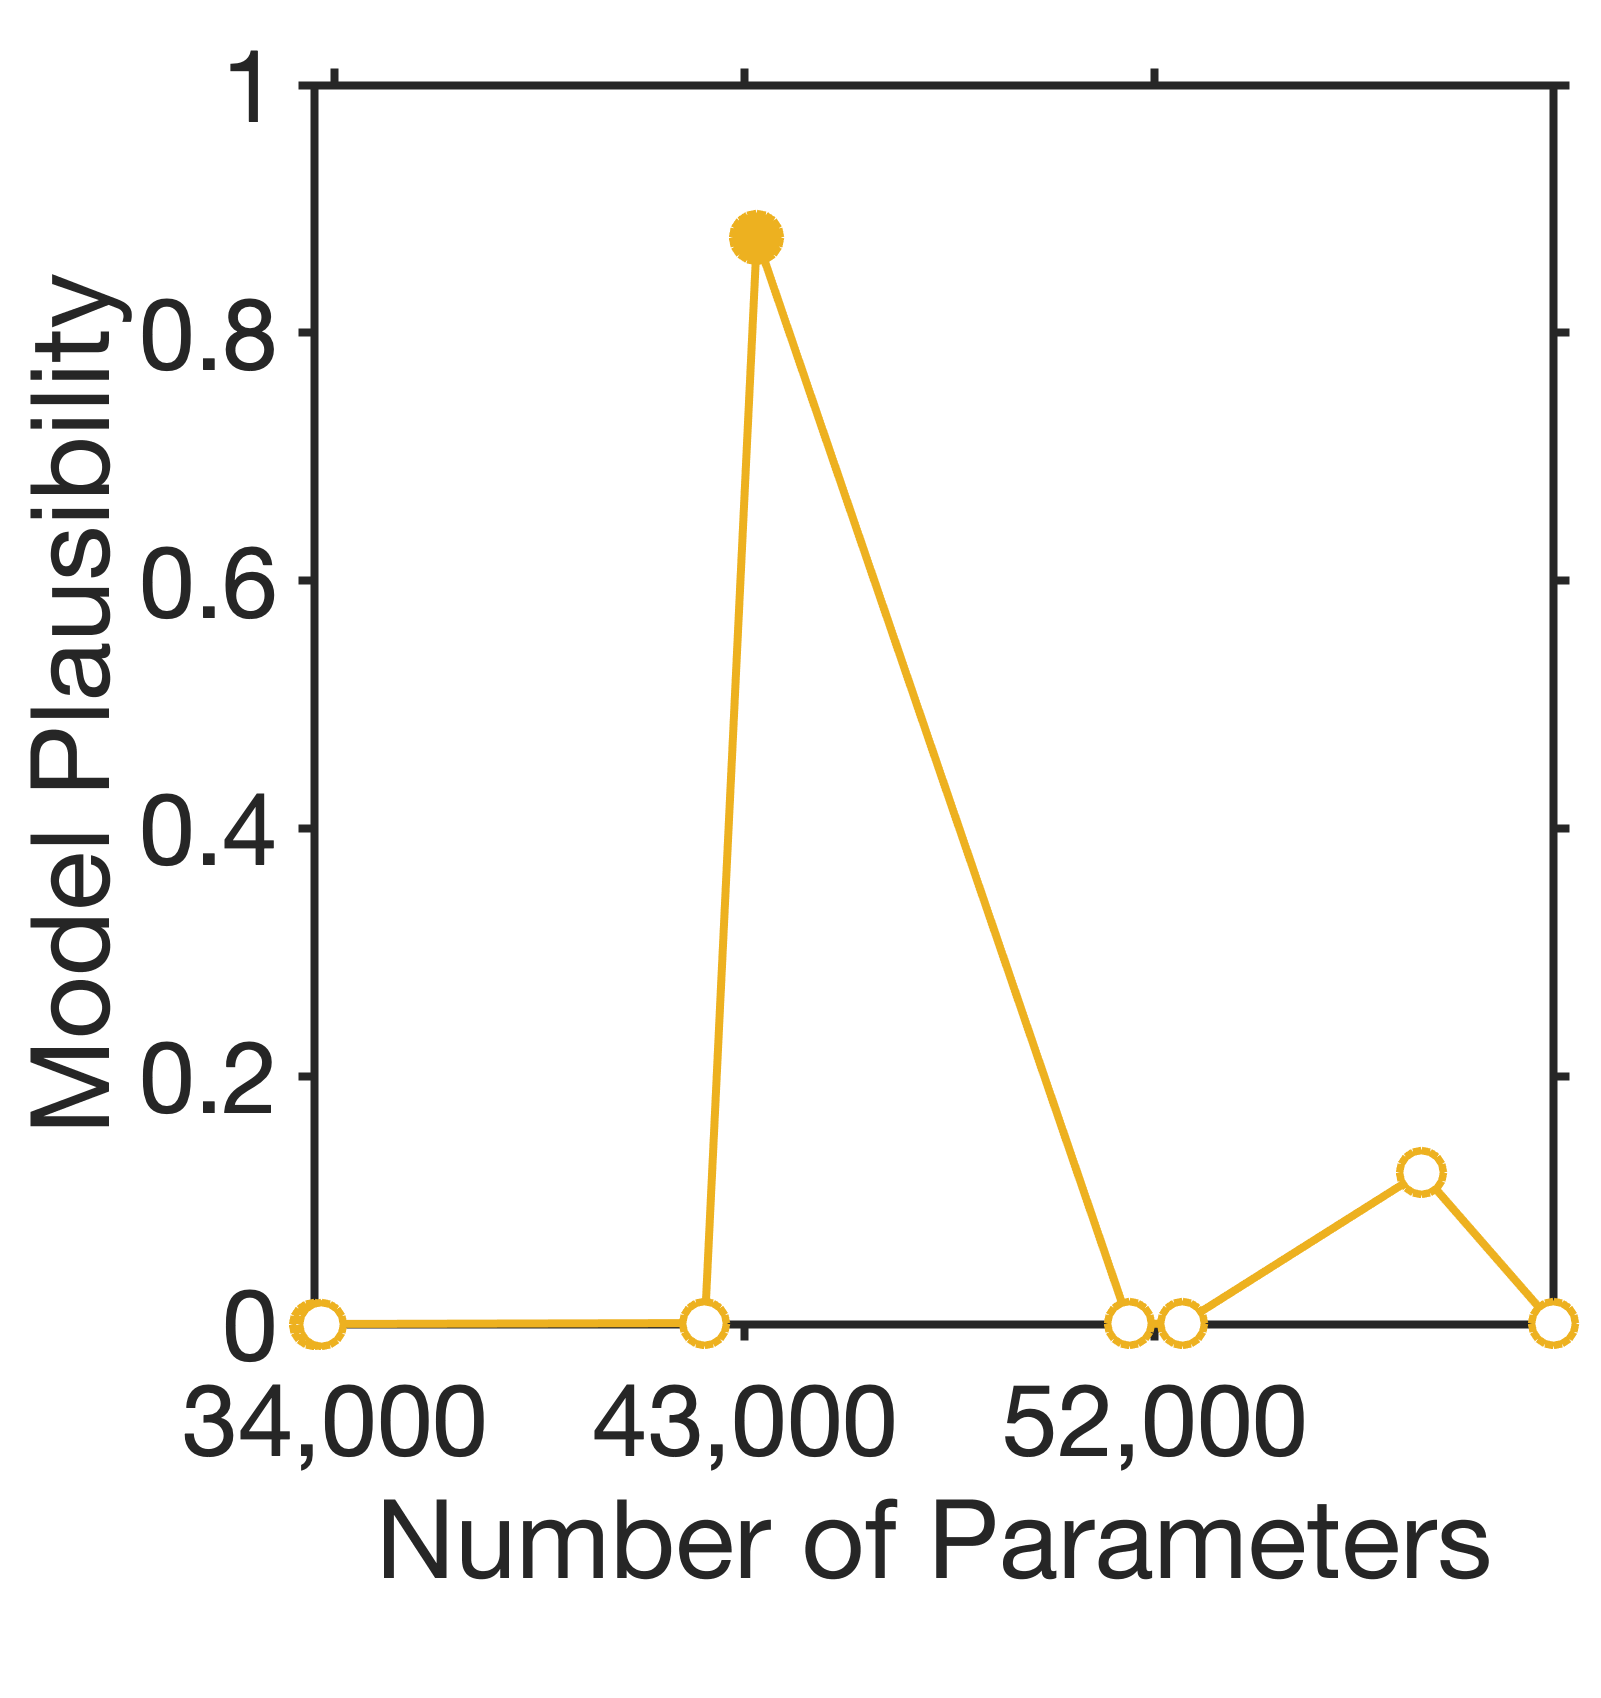
\includegraphics[width=0.19\textwidth]{Figures_manuscript/cat2_fold3.png}\hfill
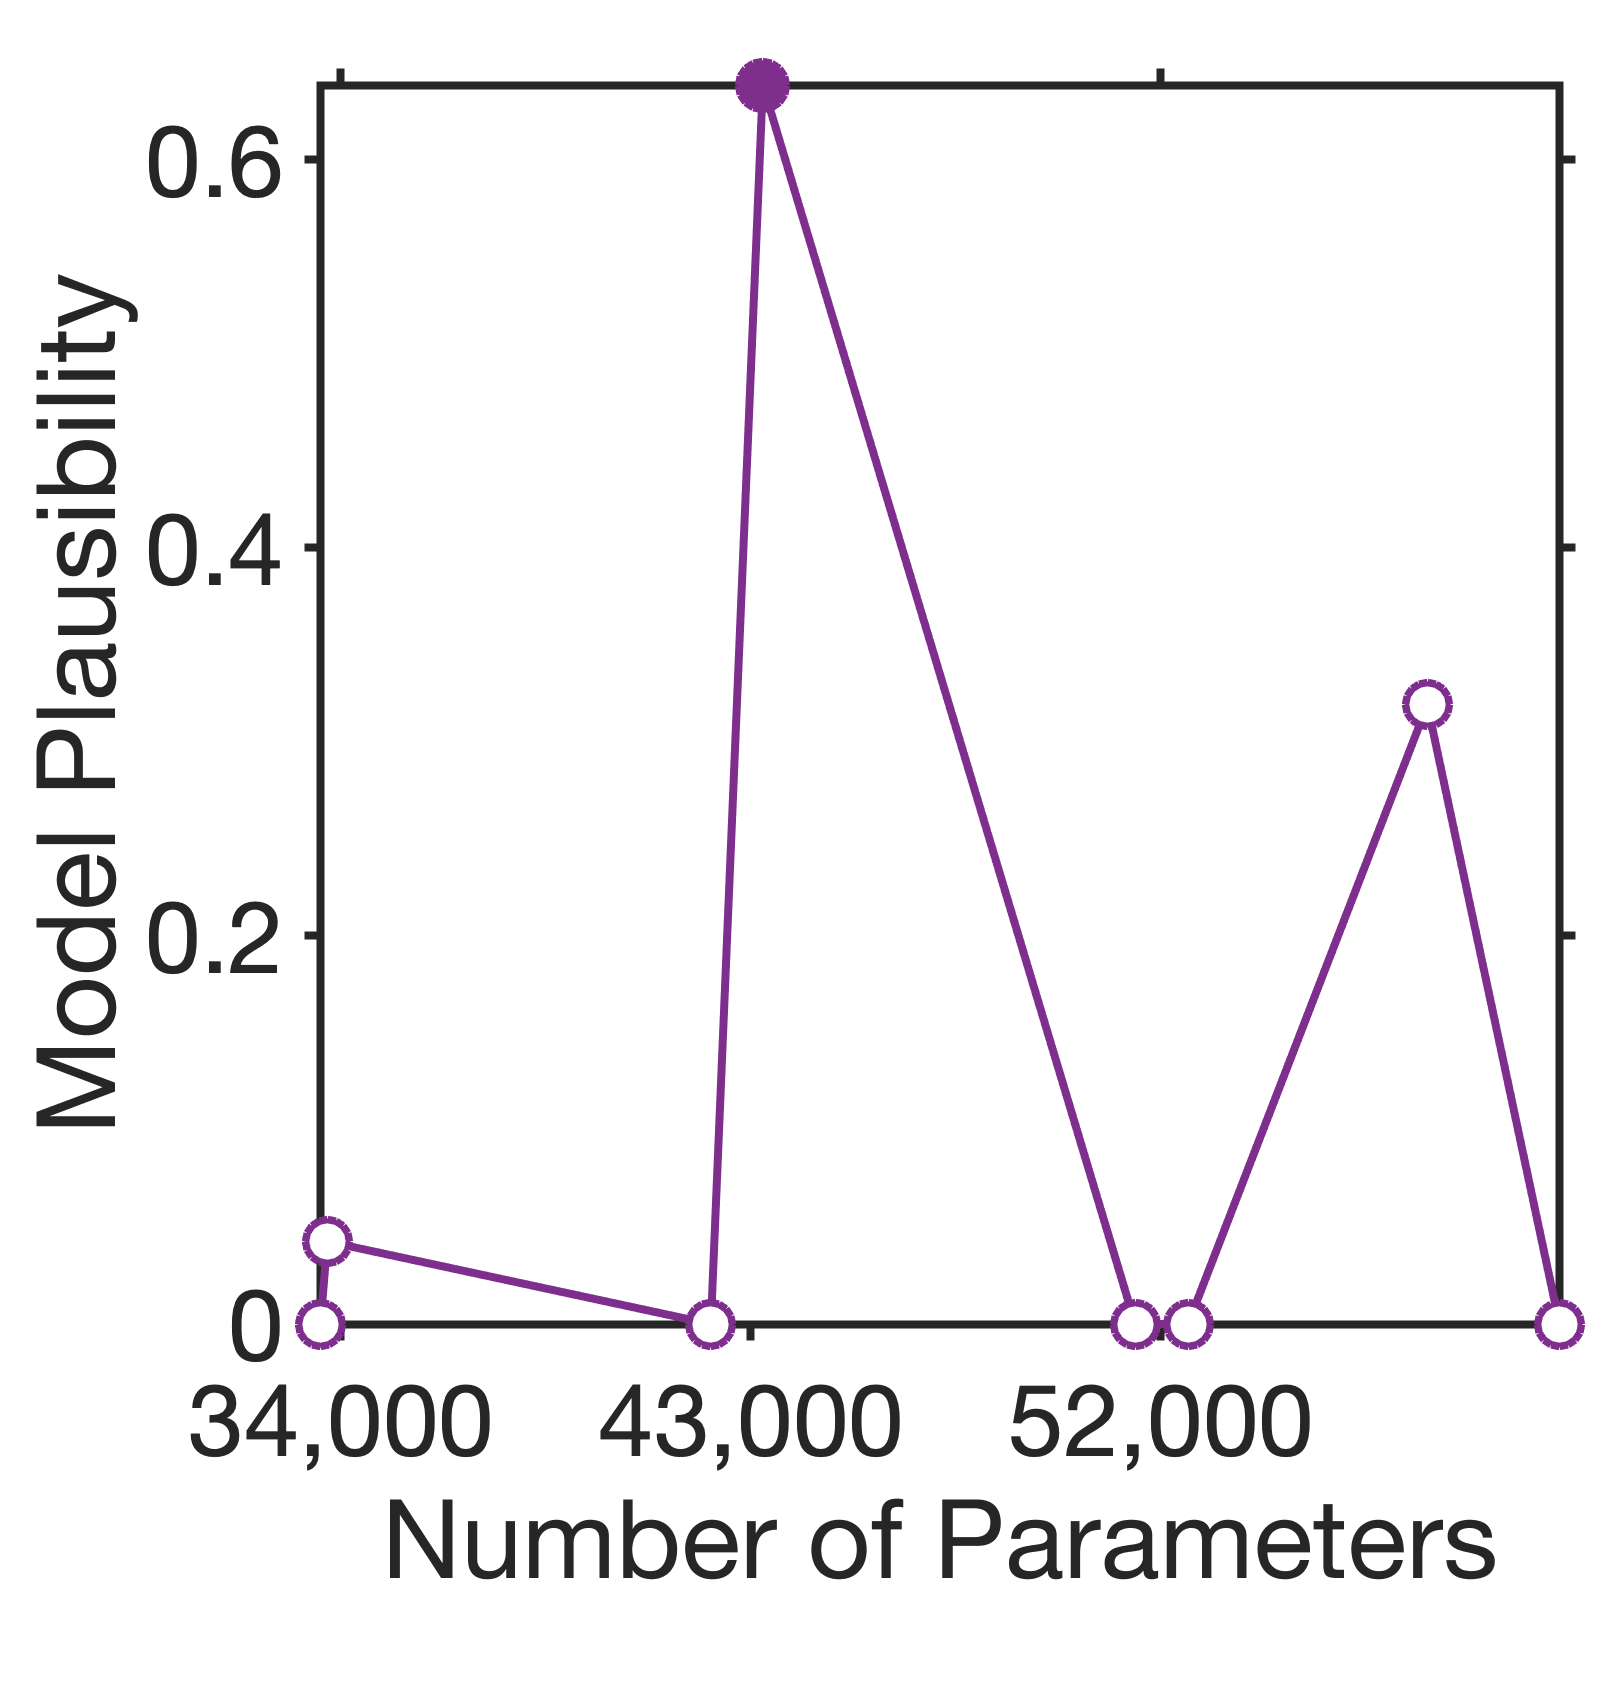
\includegraphics[width=0.19\textwidth]{Figures_manuscript/cat2_fold4.png}\hfill
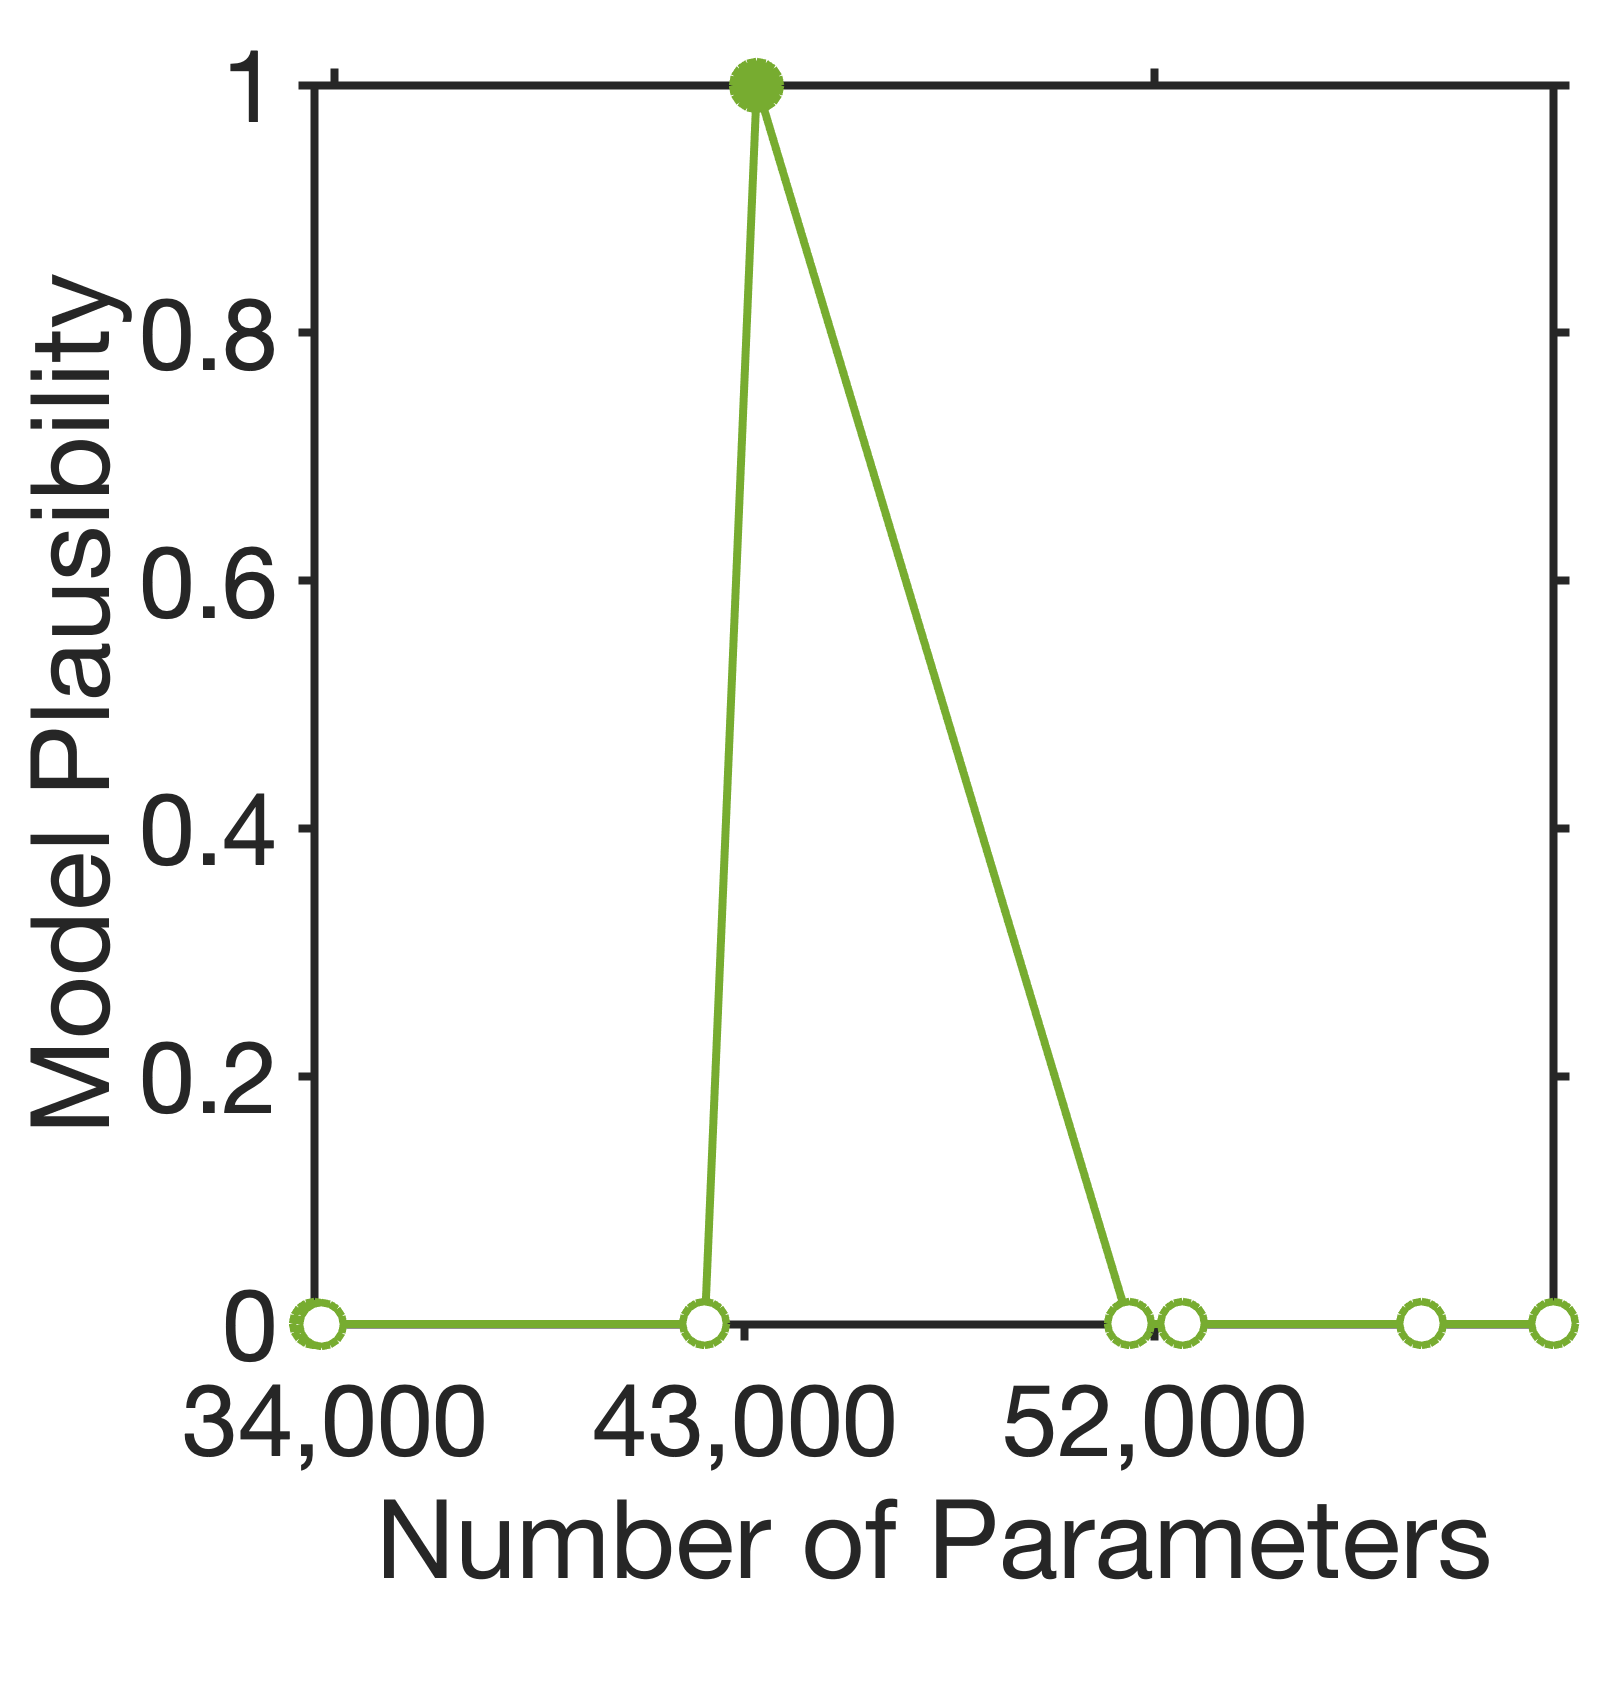
\includegraphics[width=0.19\textwidth]{Figures_manuscript/cat2_fold5.png}
\\
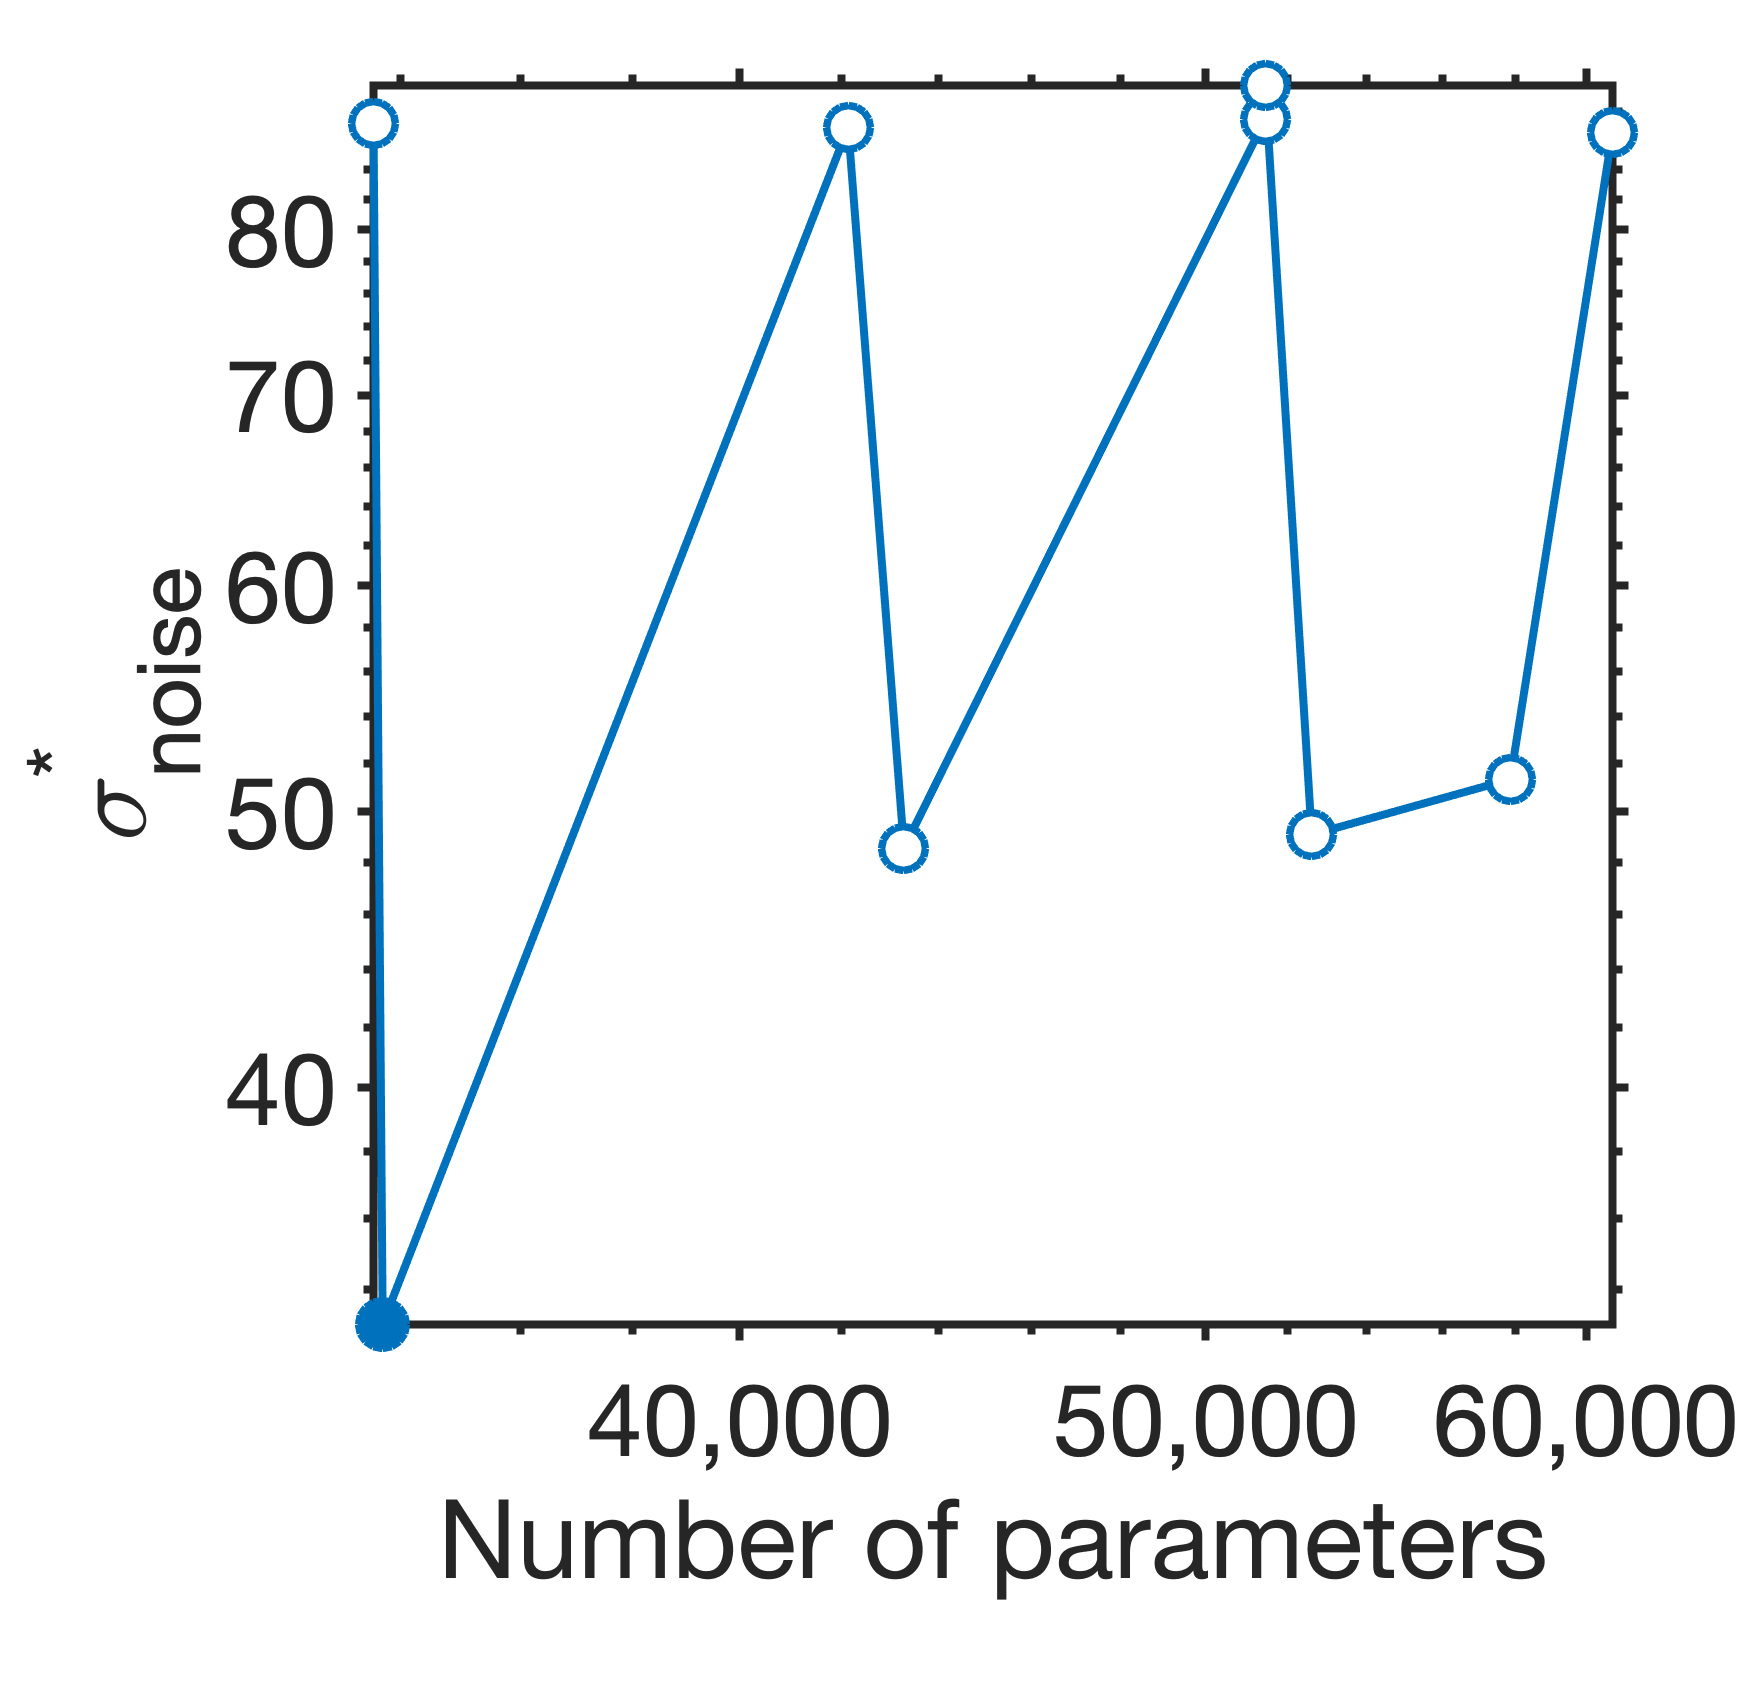
\includegraphics[width=0.19\textwidth]{Figures_manuscript/cat2_fold1_noise.png}\hfill
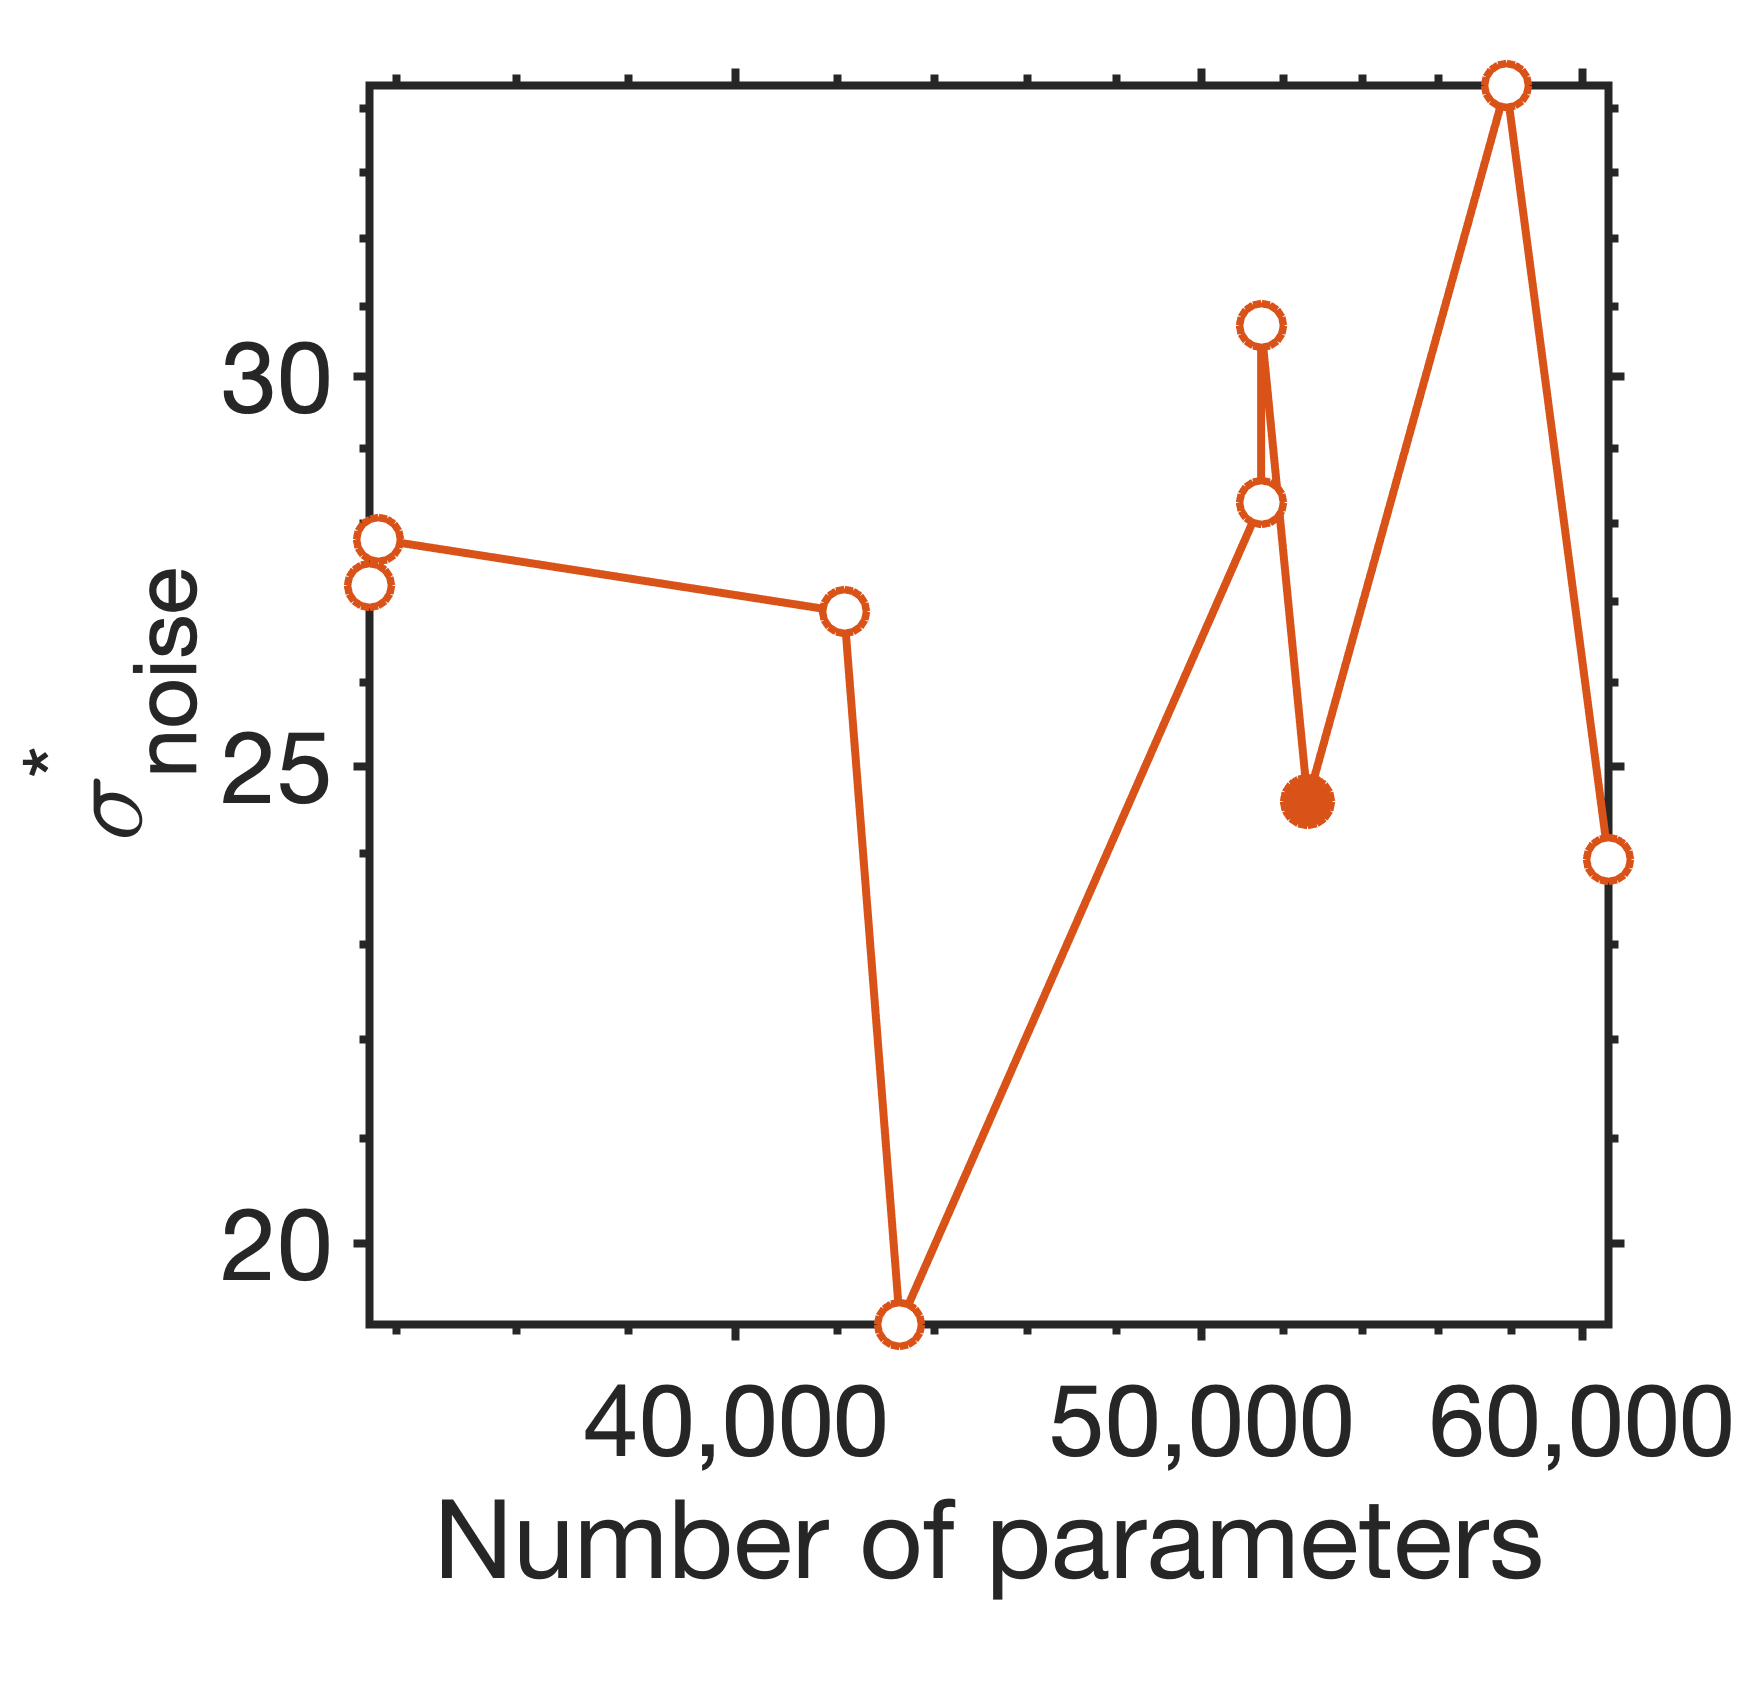
\includegraphics[width=0.19\textwidth]{Figures_manuscript/cat2_fold2_noise.png}\hfill
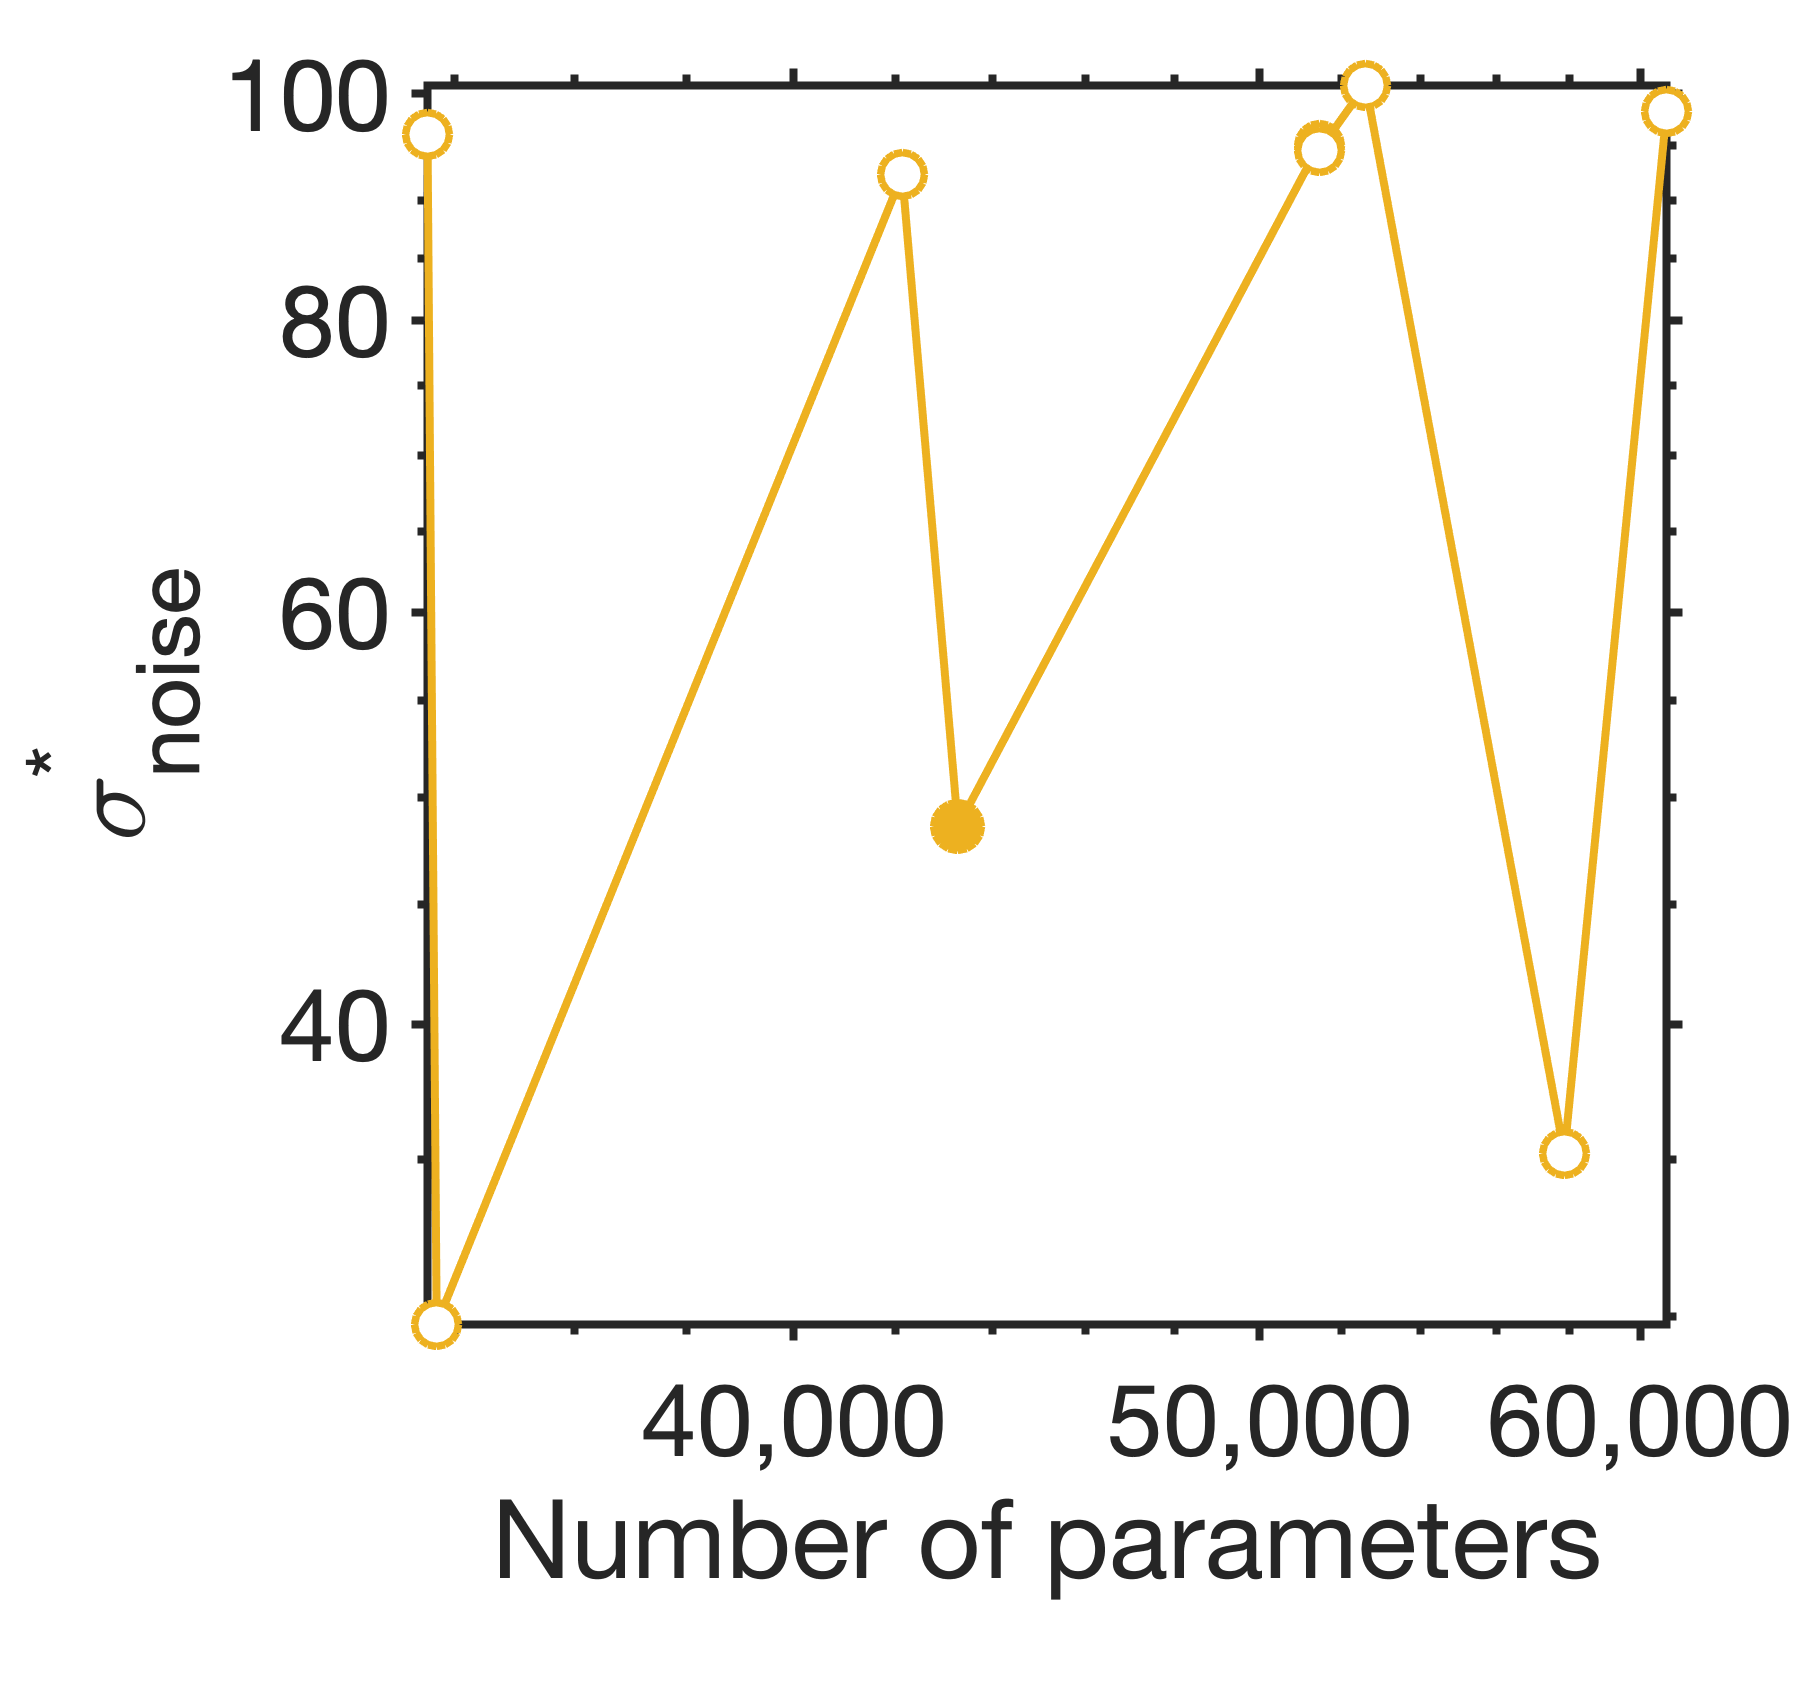
\includegraphics[width=0.19\textwidth]{Figures_manuscript/cat2_fold3_noise.png}\hfill
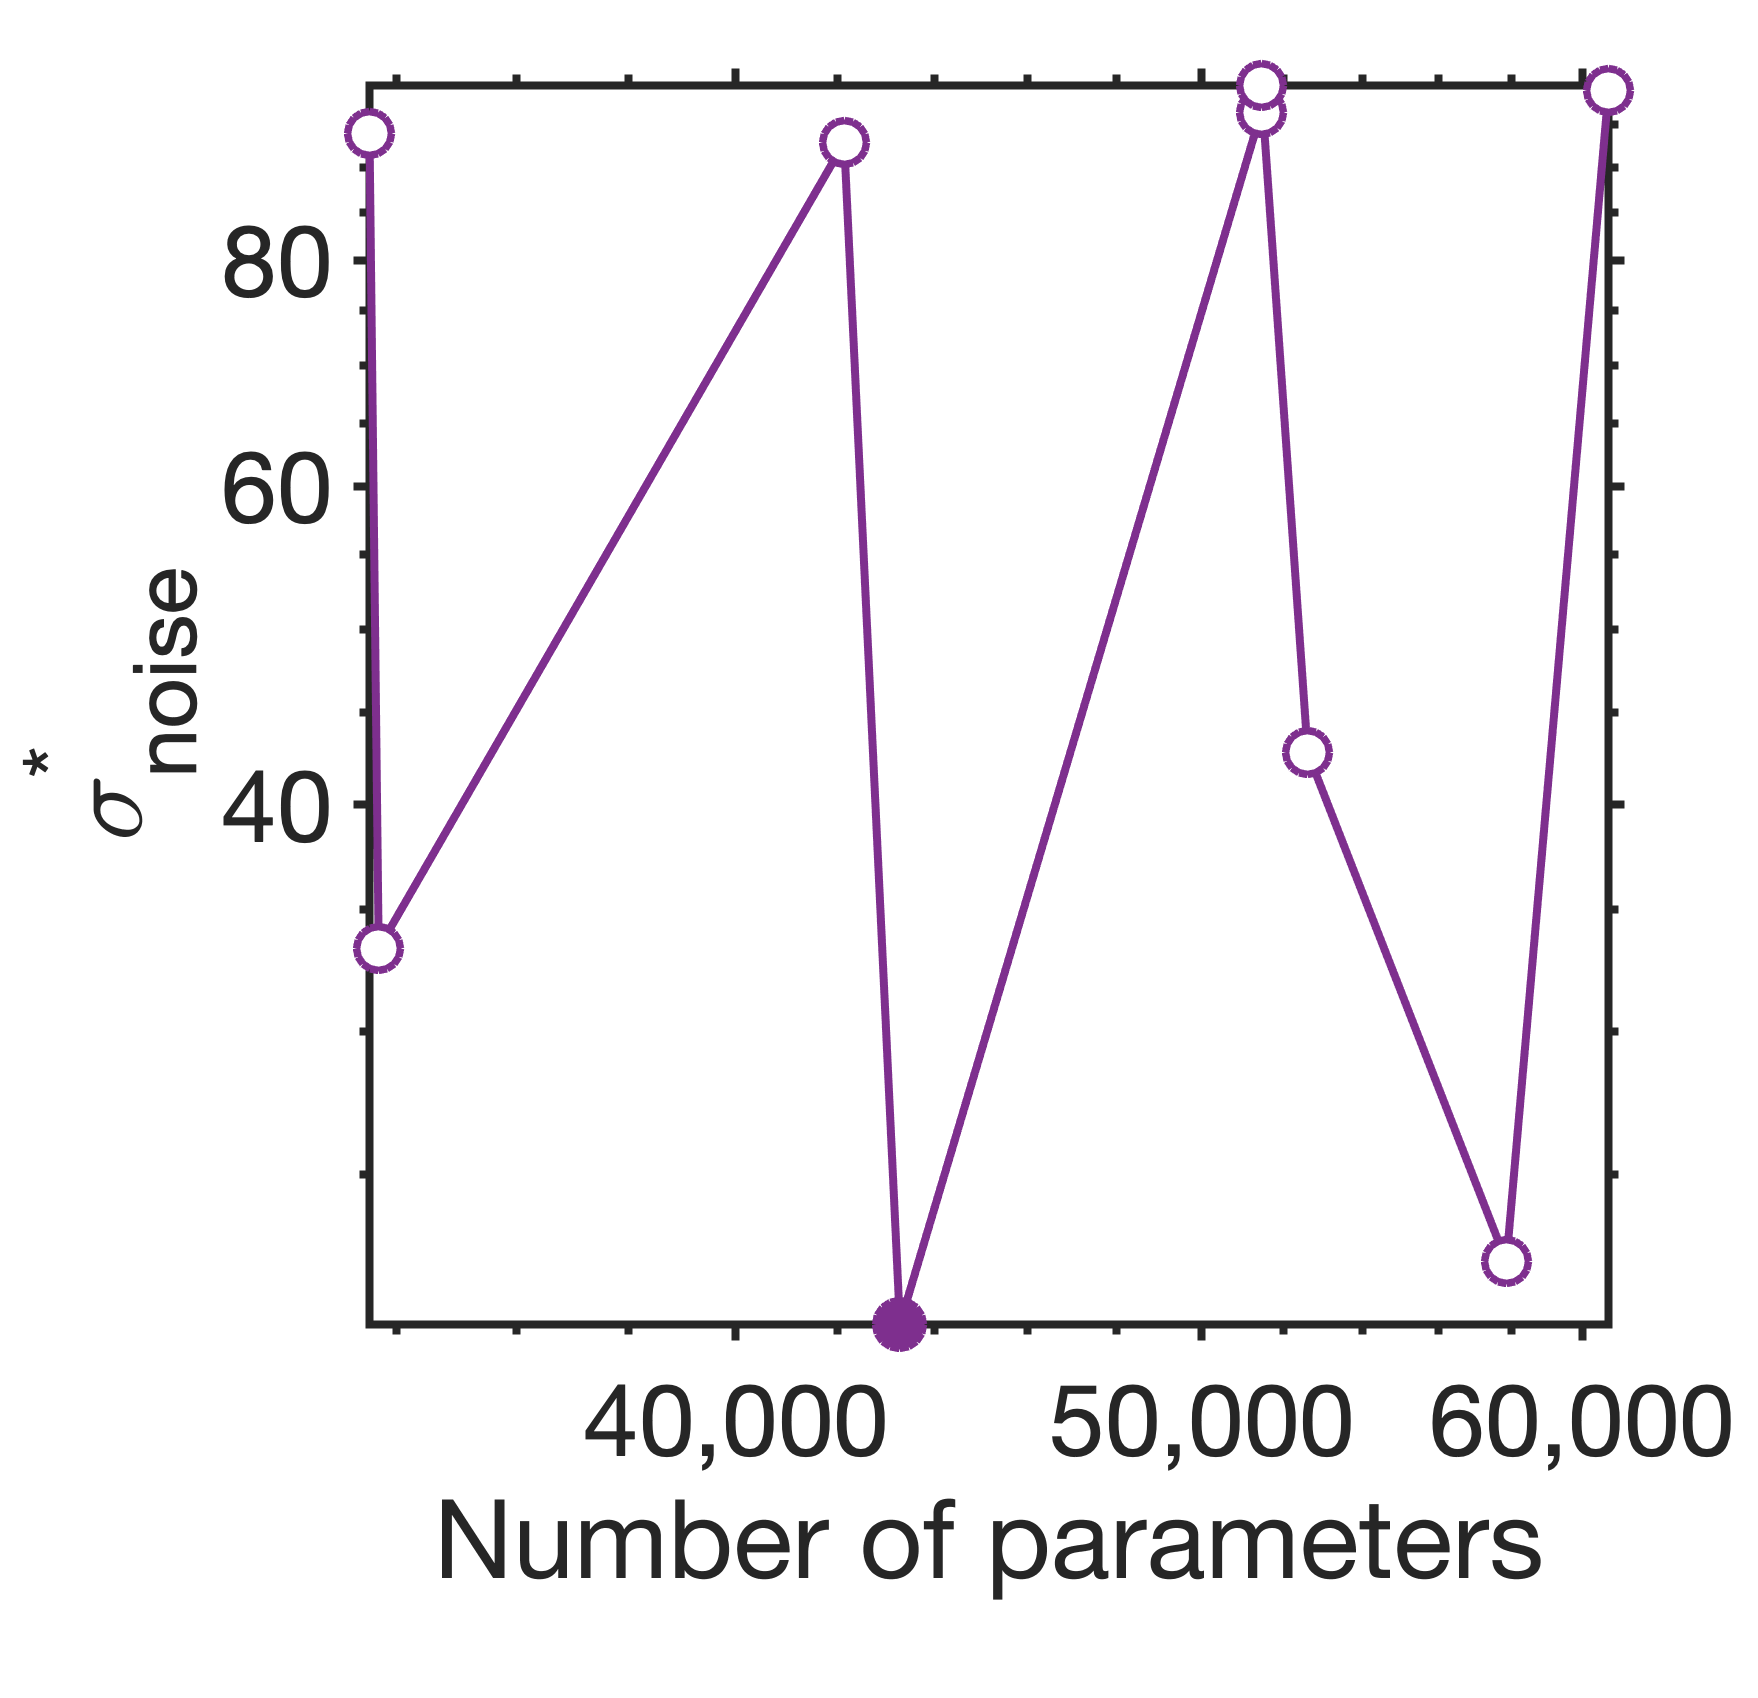
\includegraphics[width=0.19\textwidth]{Figures_manuscript/cat2_fold4_noise.png}\hfill
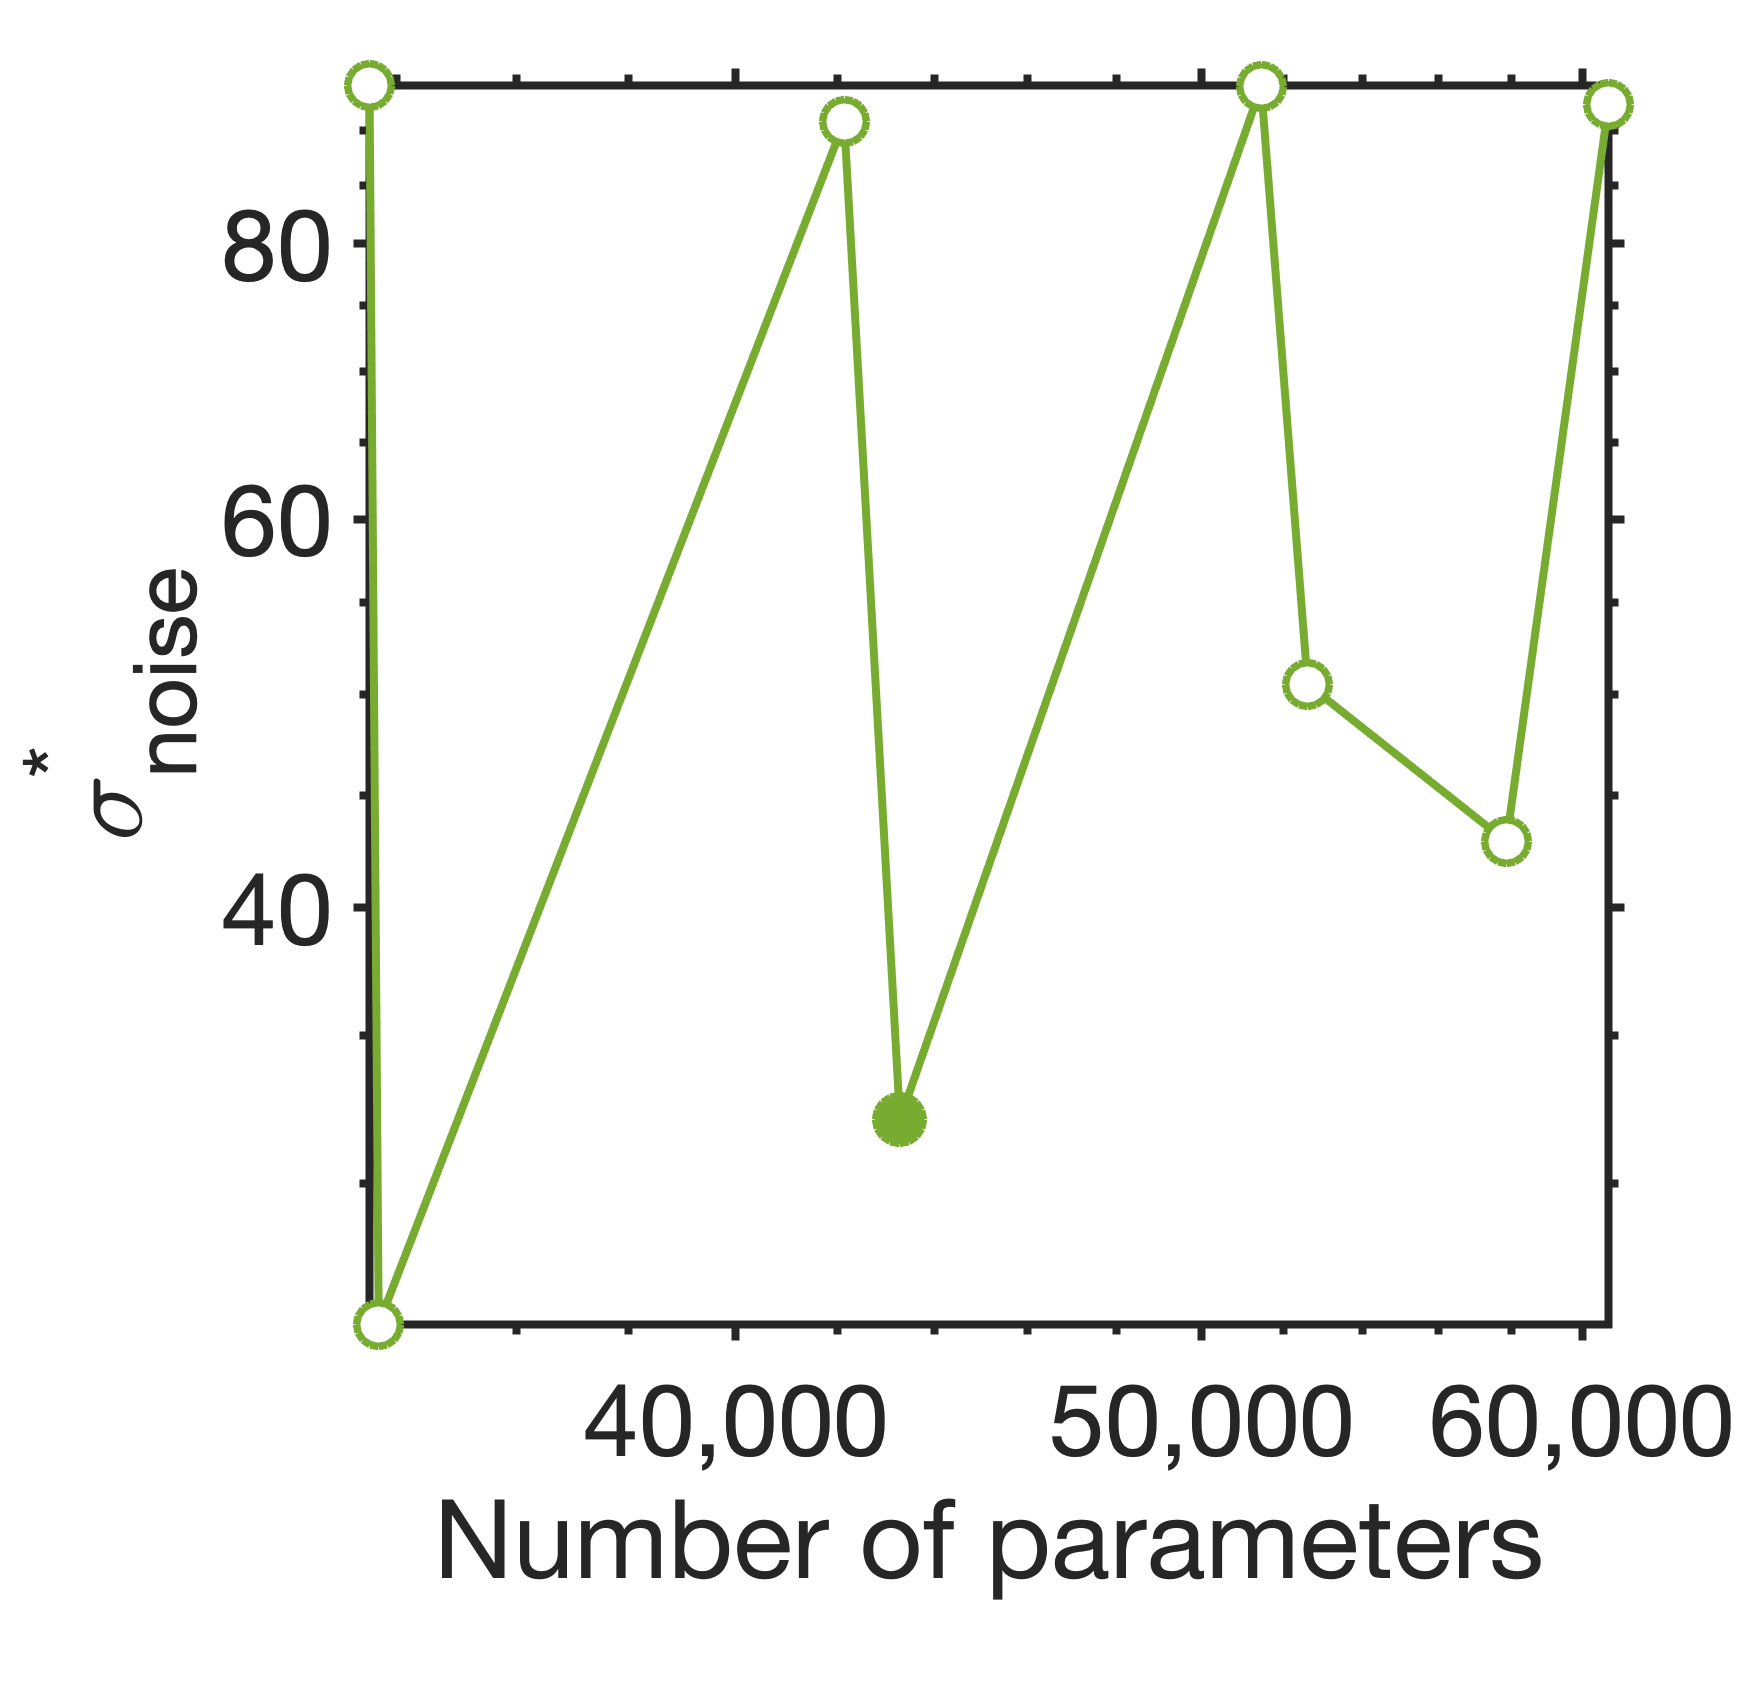
\includegraphics[width=0.19\textwidth]{Figures_manuscript/cat2_fold5_noise.png}
\vspace{-0.1in}
\\ (a)\\
  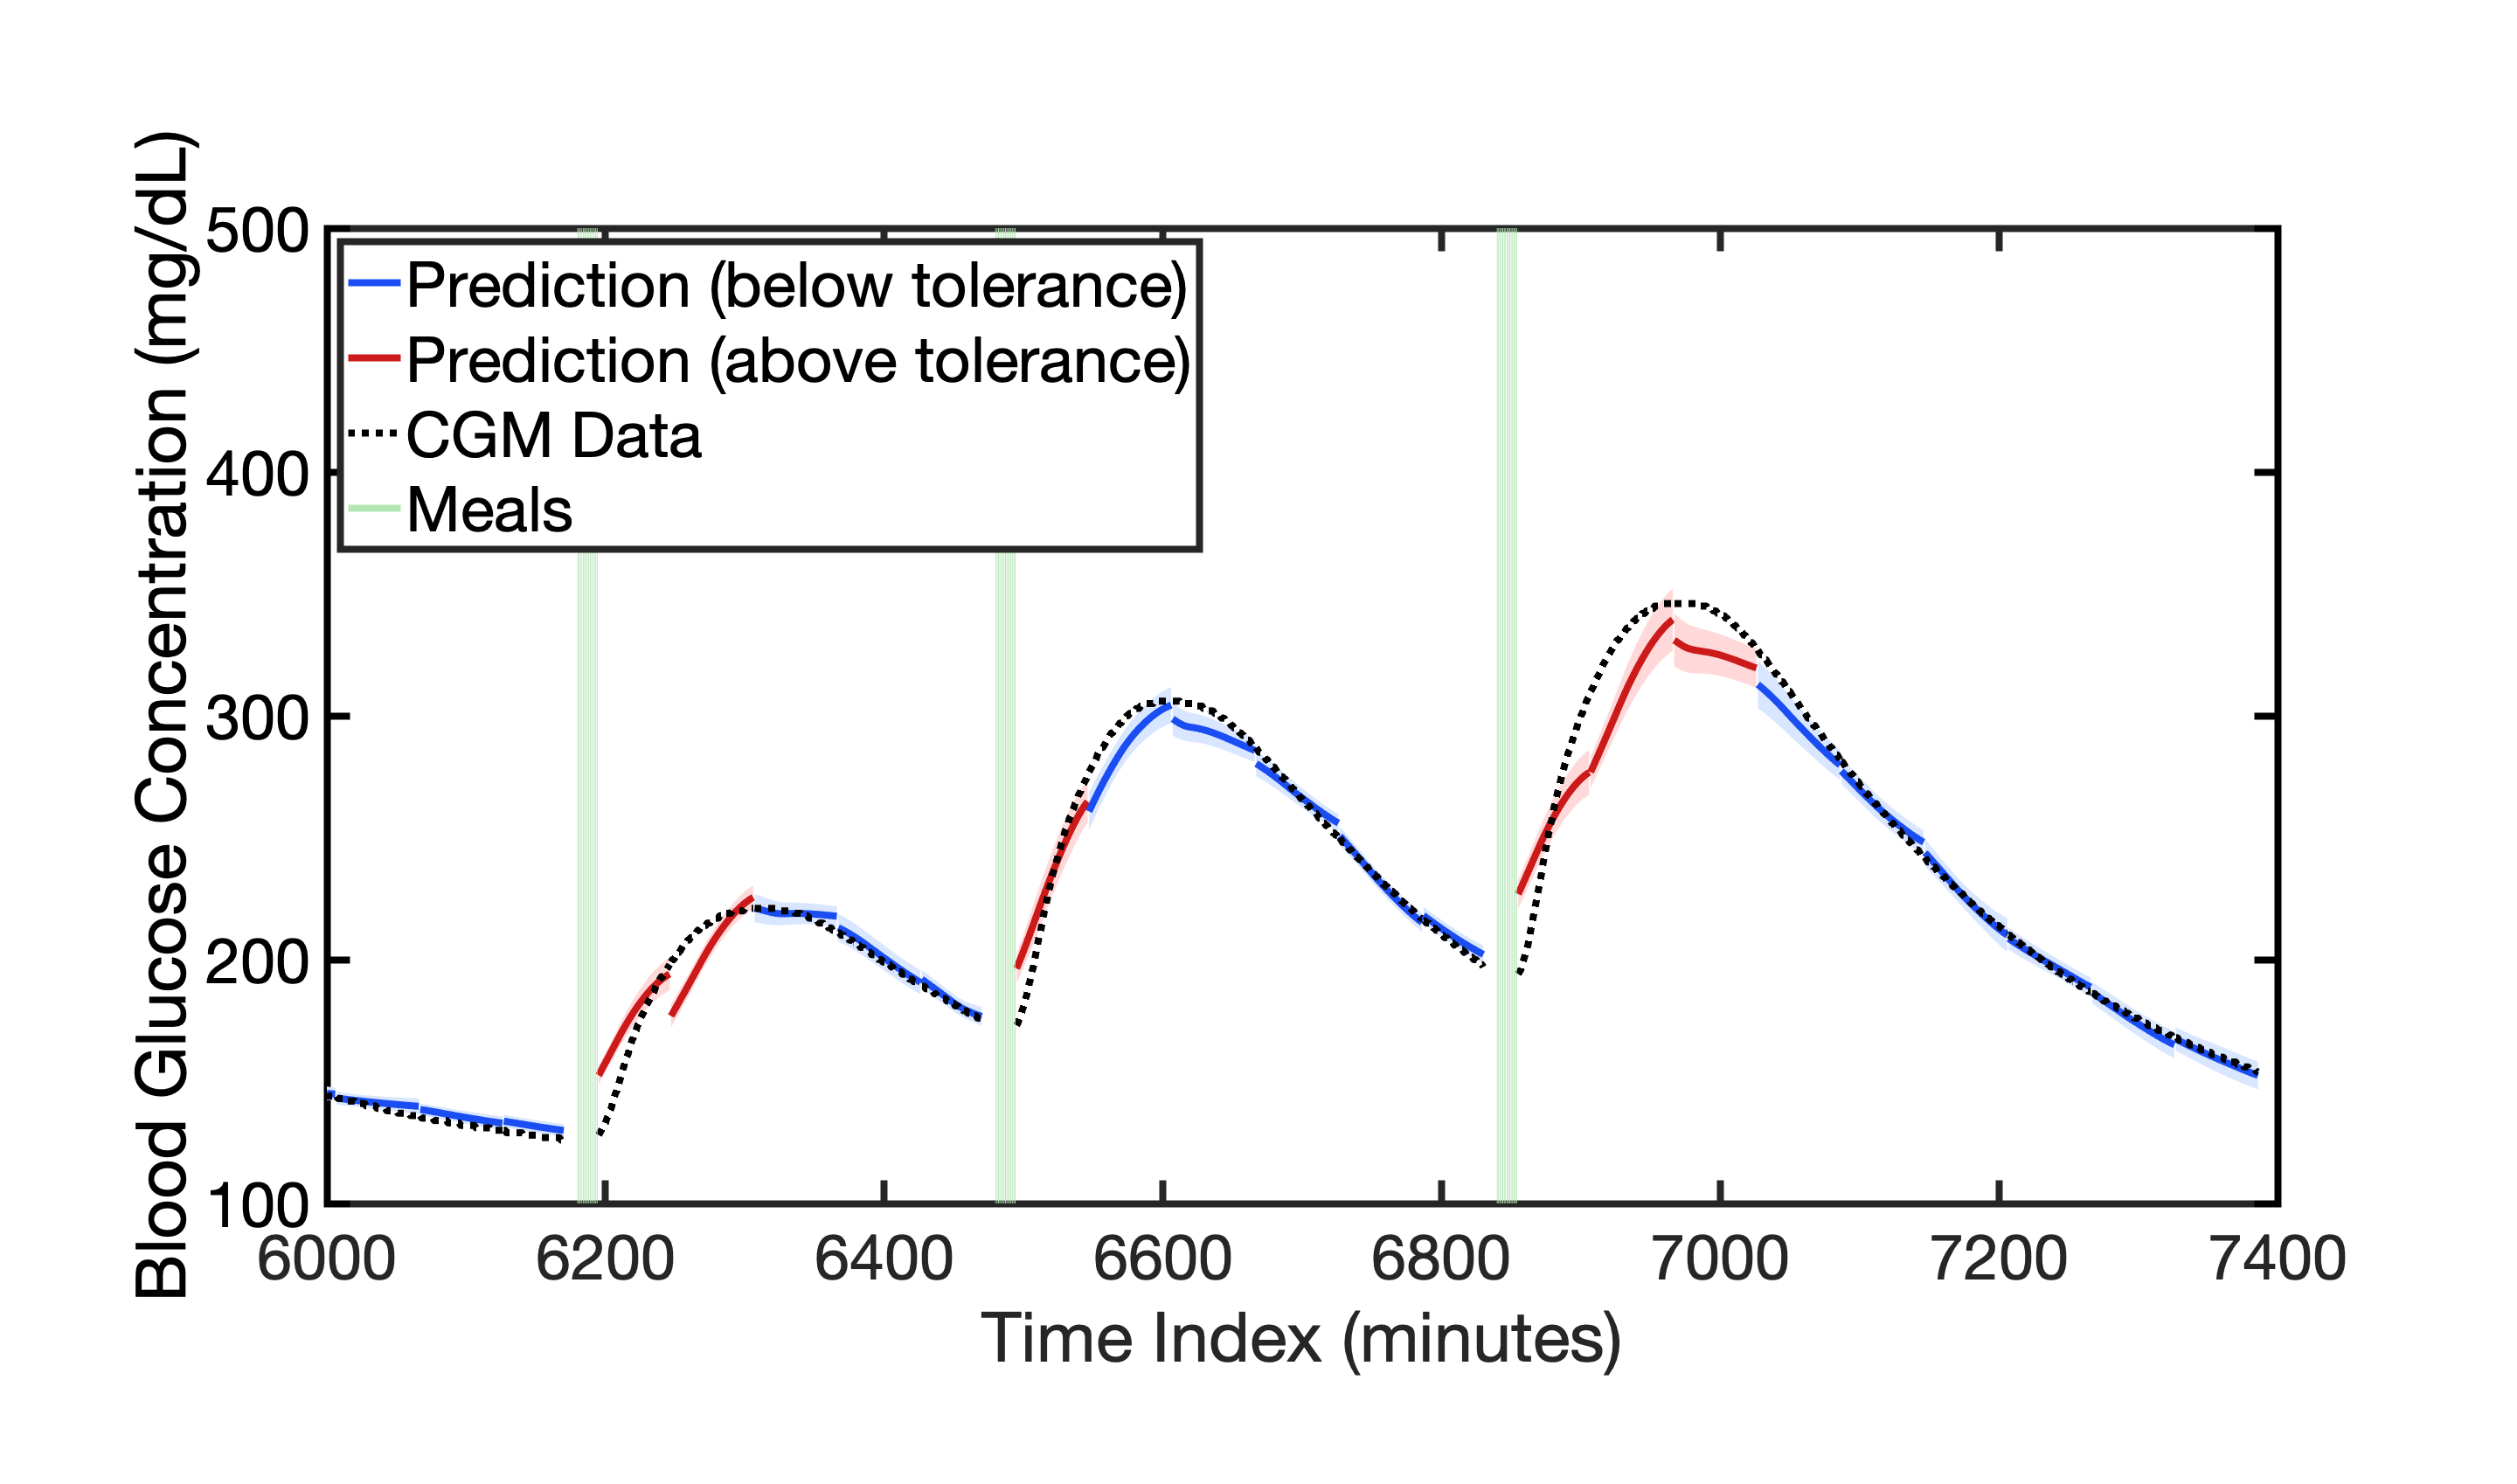
\includegraphics[width=0.43\linewidth]{Figures_manuscript/cat2_p9_c2.png}
~
  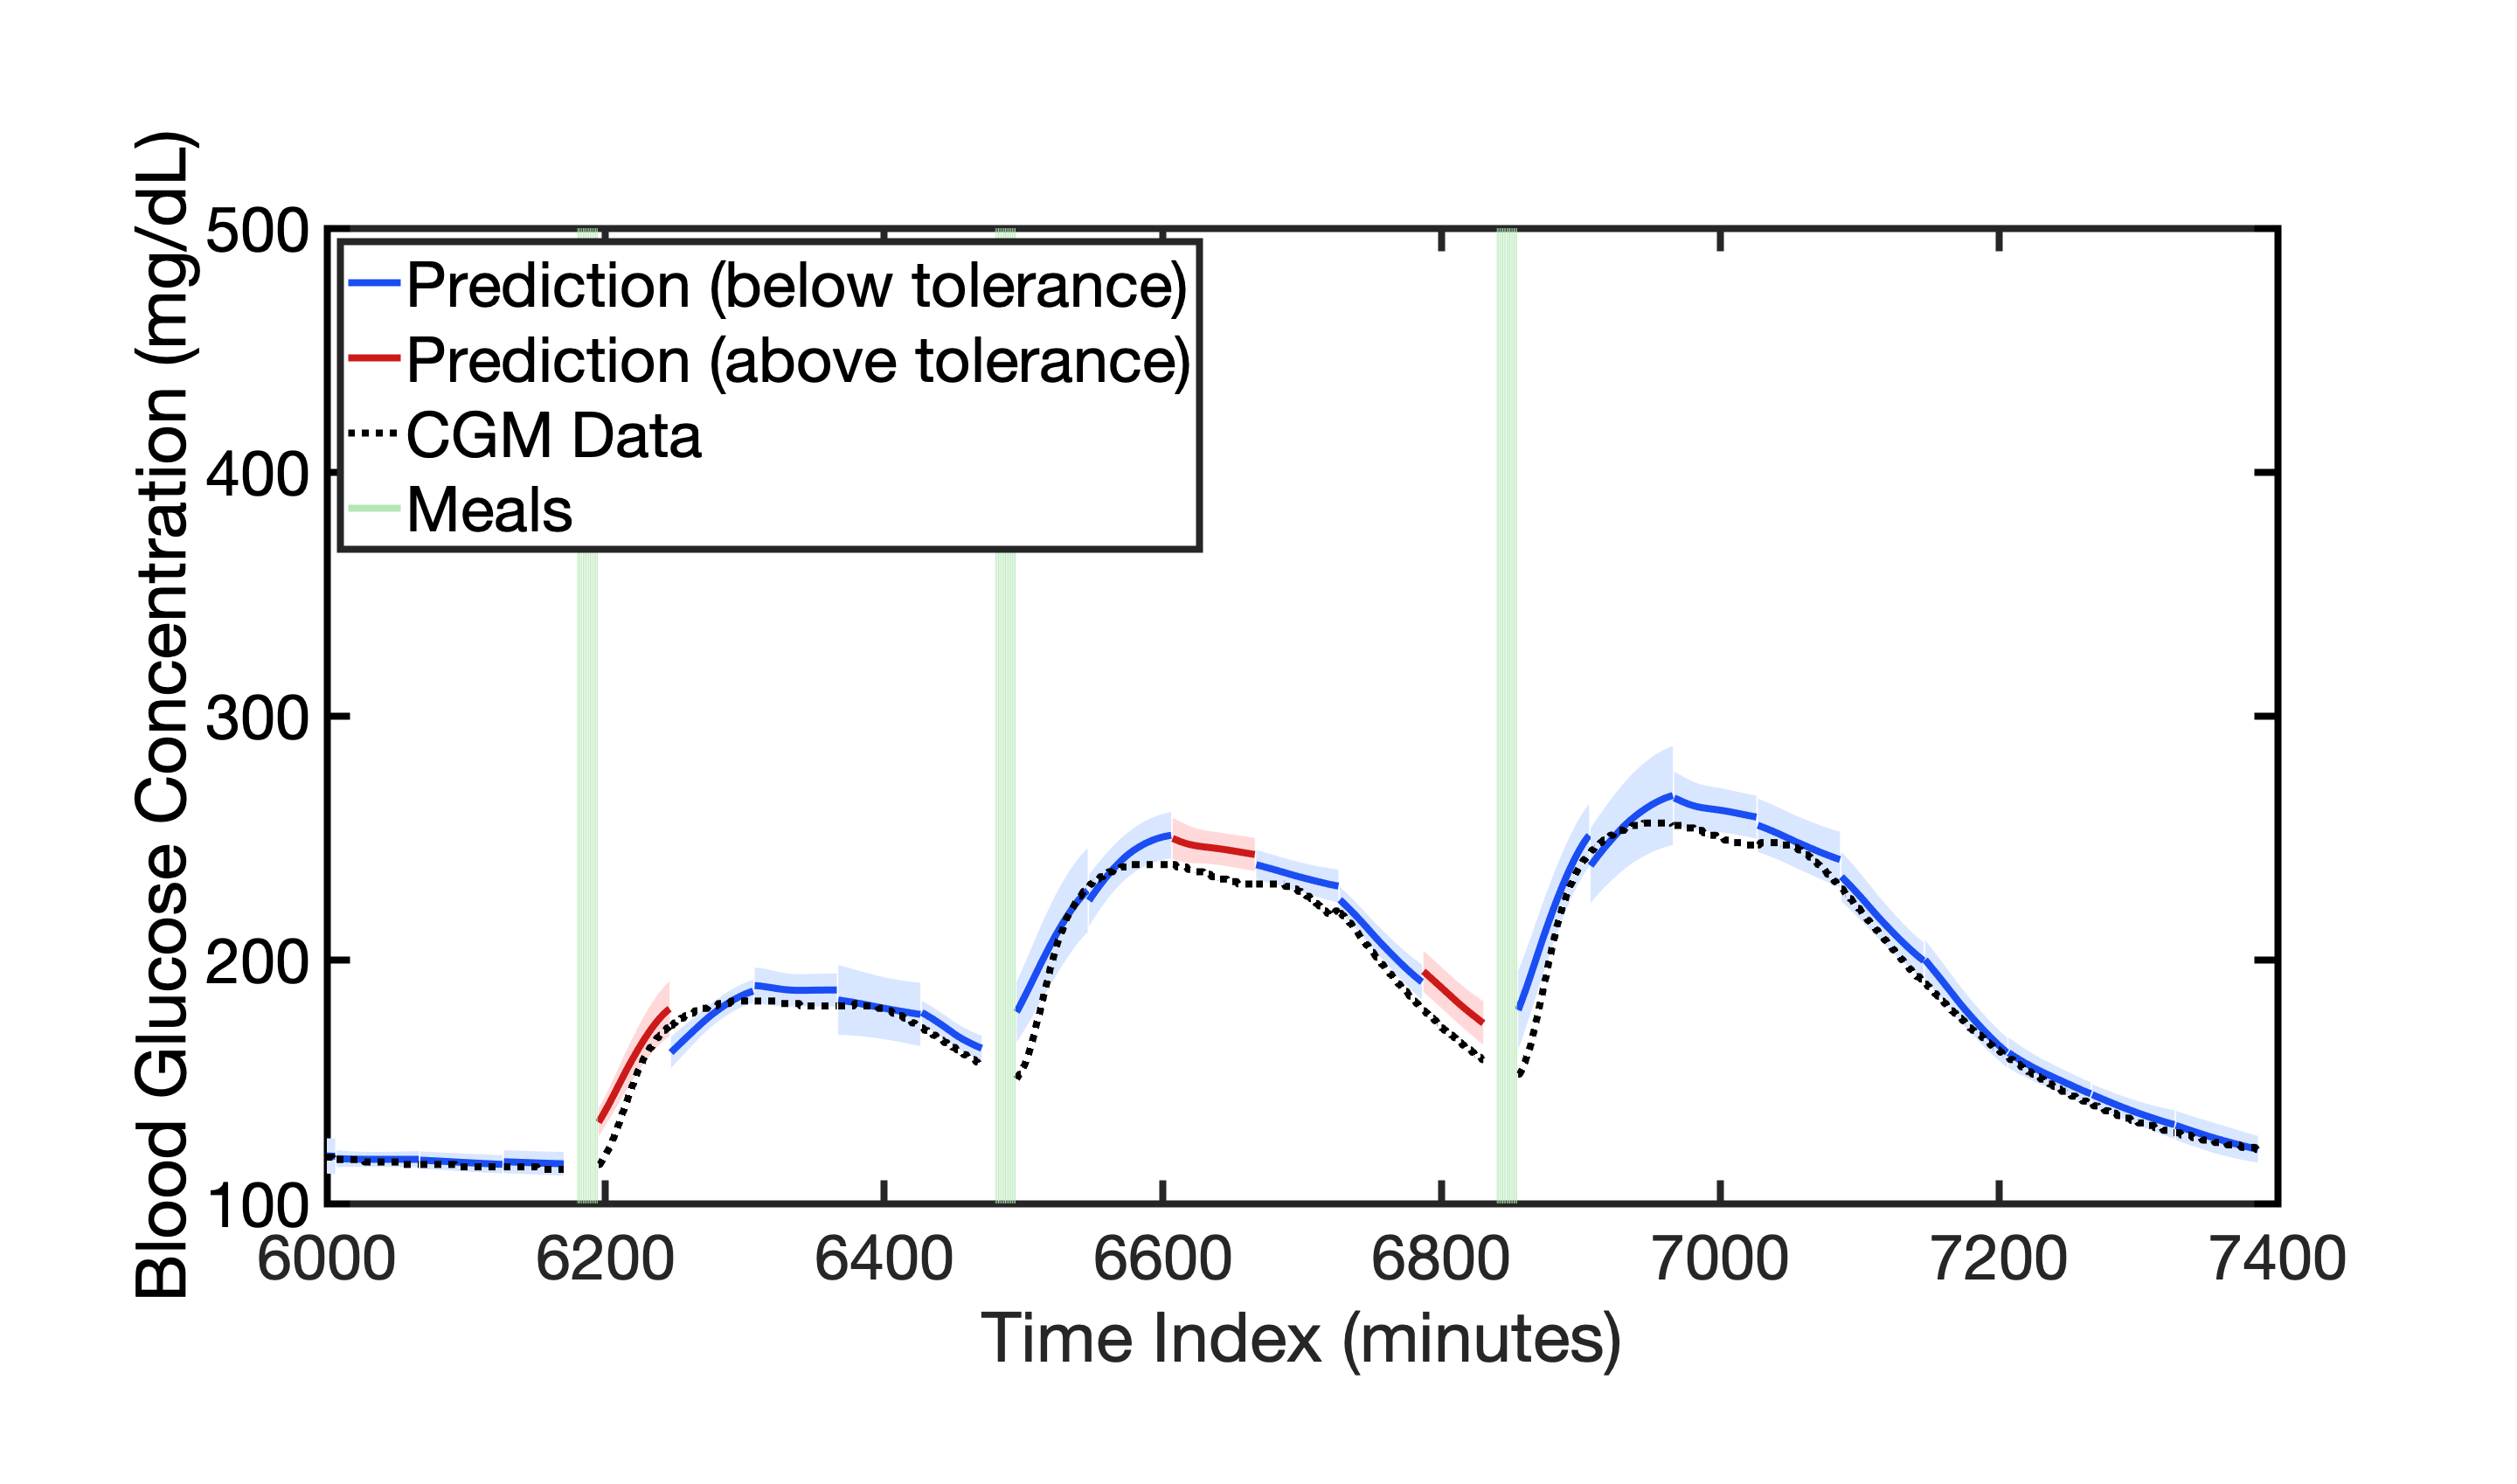
\includegraphics[width=0.43\linewidth]{Figures_manuscript/cat2_p10_c2.png}
  \vspace{-0.1in}
\\ (b)  \hspace{2.5in}  (c)\\
  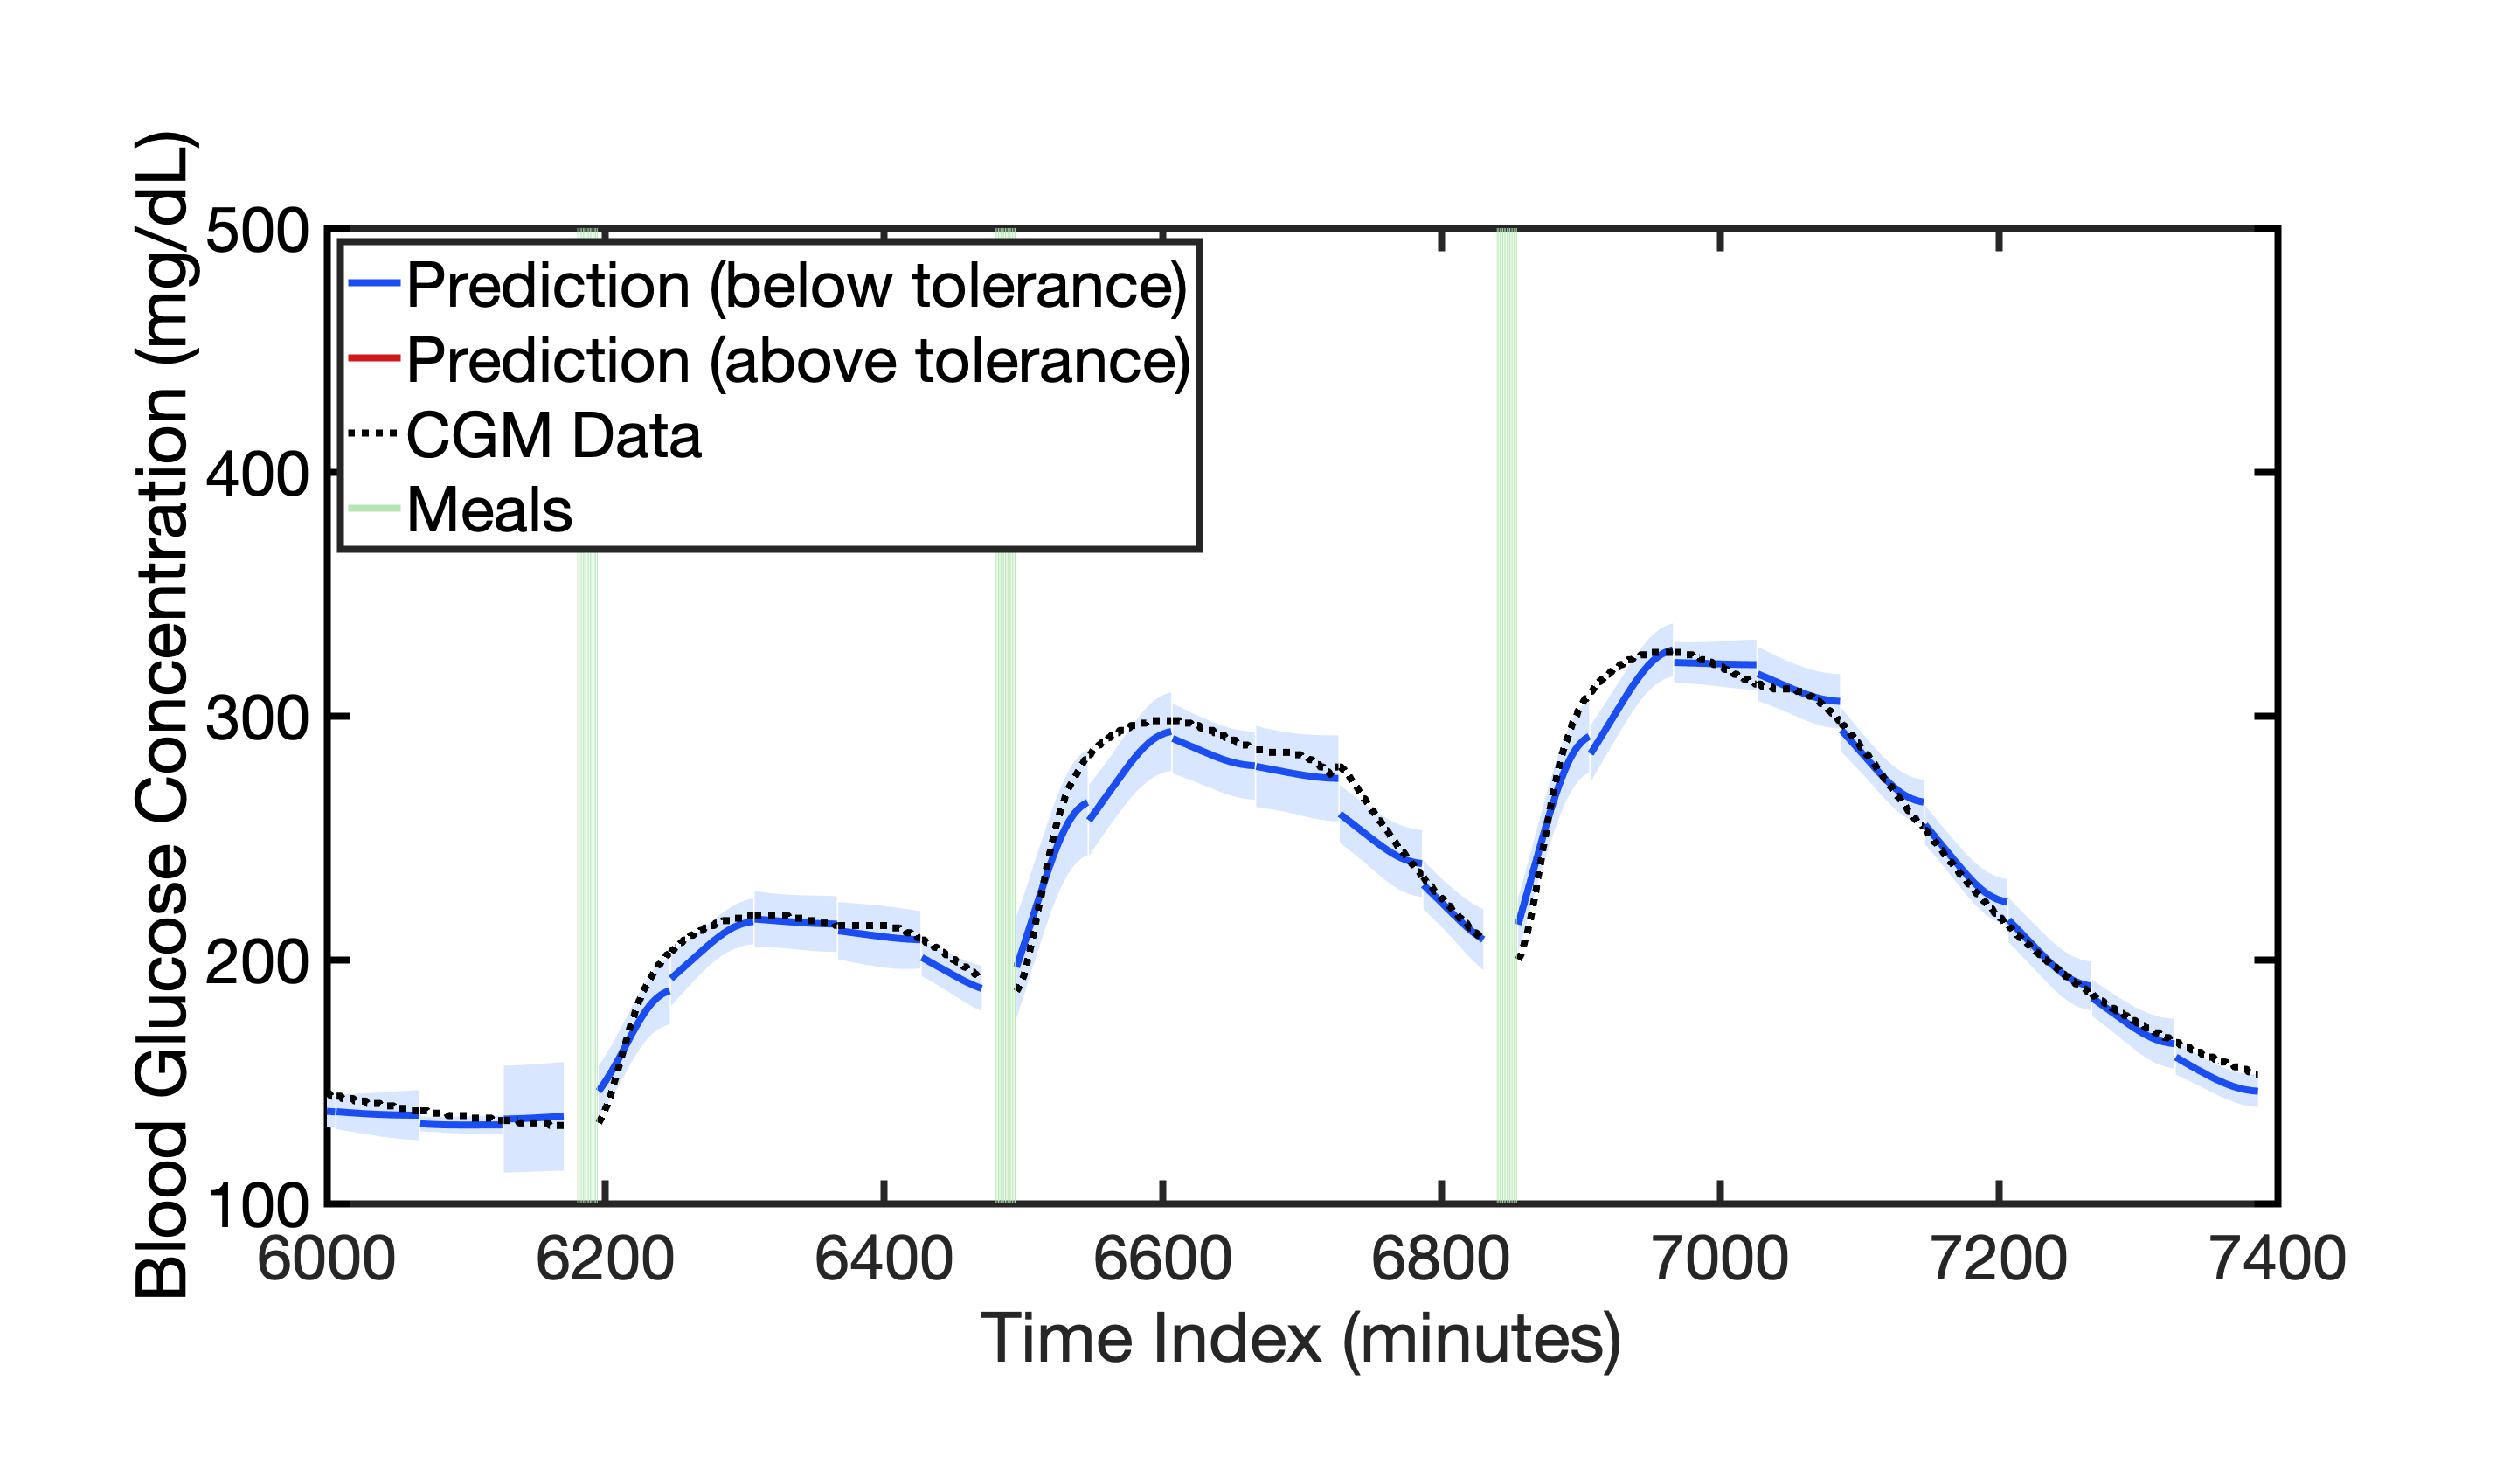
\includegraphics[width=0.43\linewidth]{Figures_manuscript/cat2_p1_c2.png}
  ~
  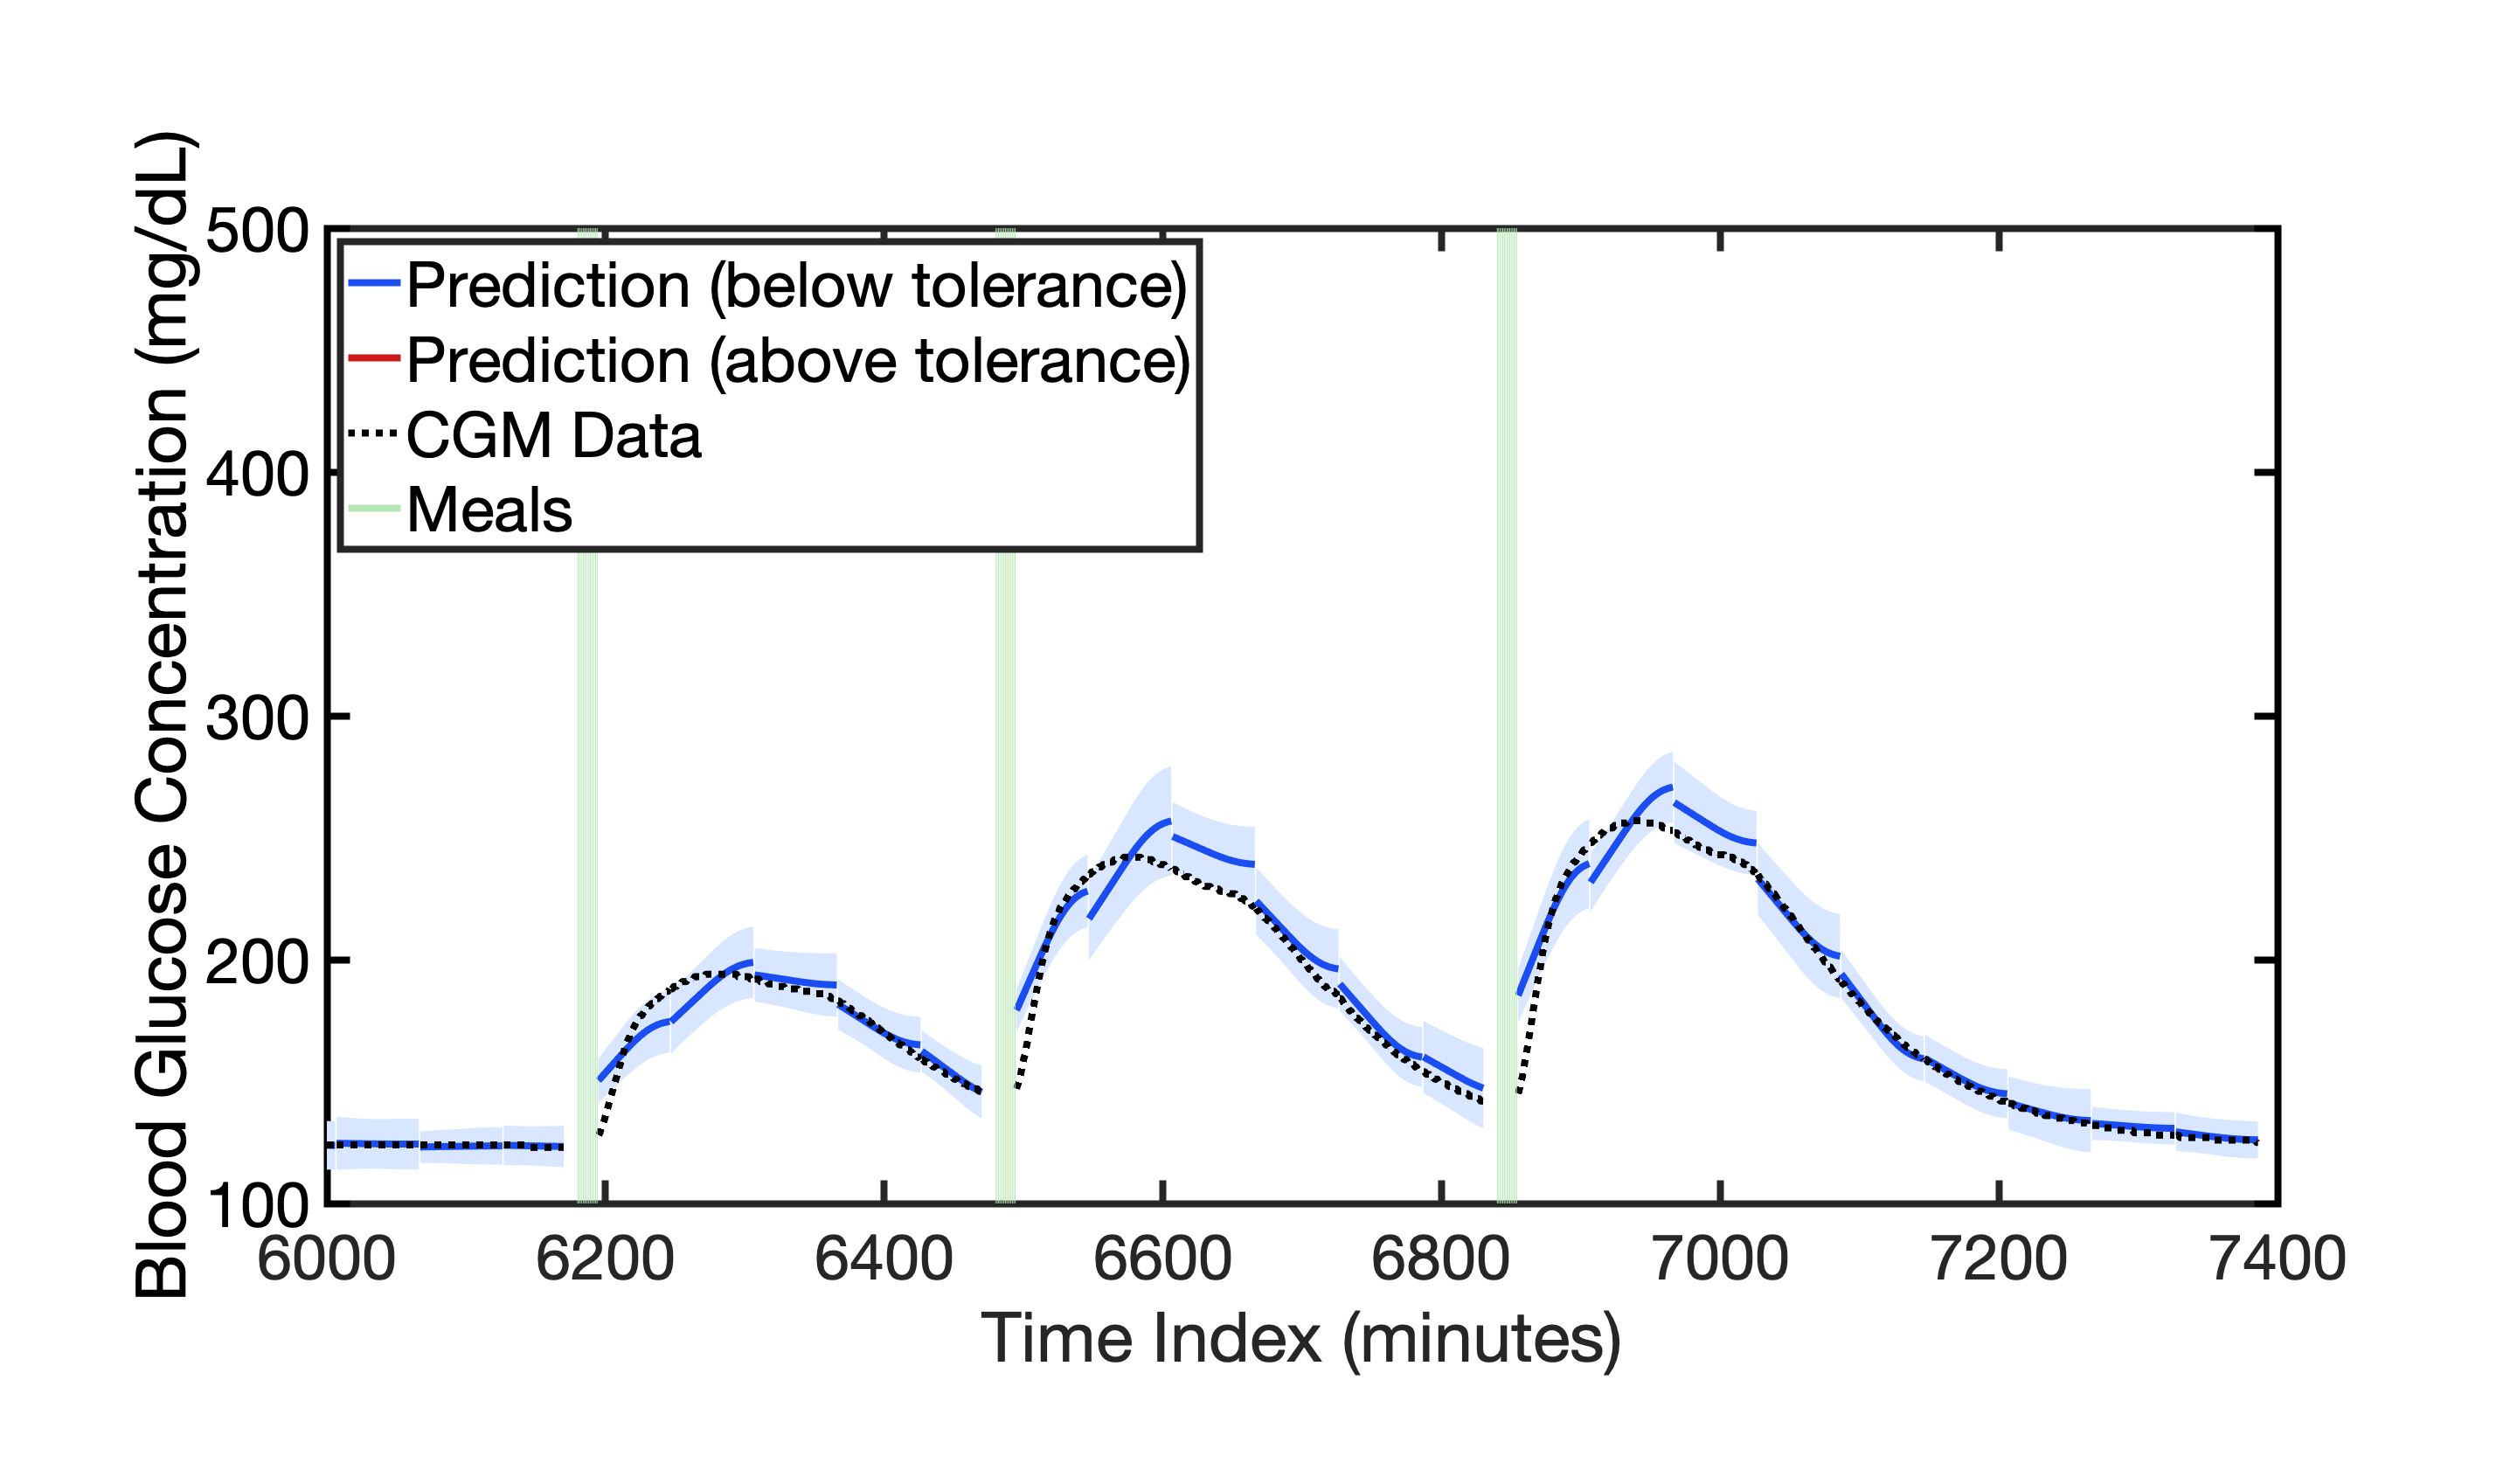
\includegraphics[width=0.43\linewidth]{Figures_manuscript/cat2_p2_c2.png}
  \vspace{-0.1in}
\\ (d)  \hspace{2.5in}  (e)\\
\vspace{-0.05in}
  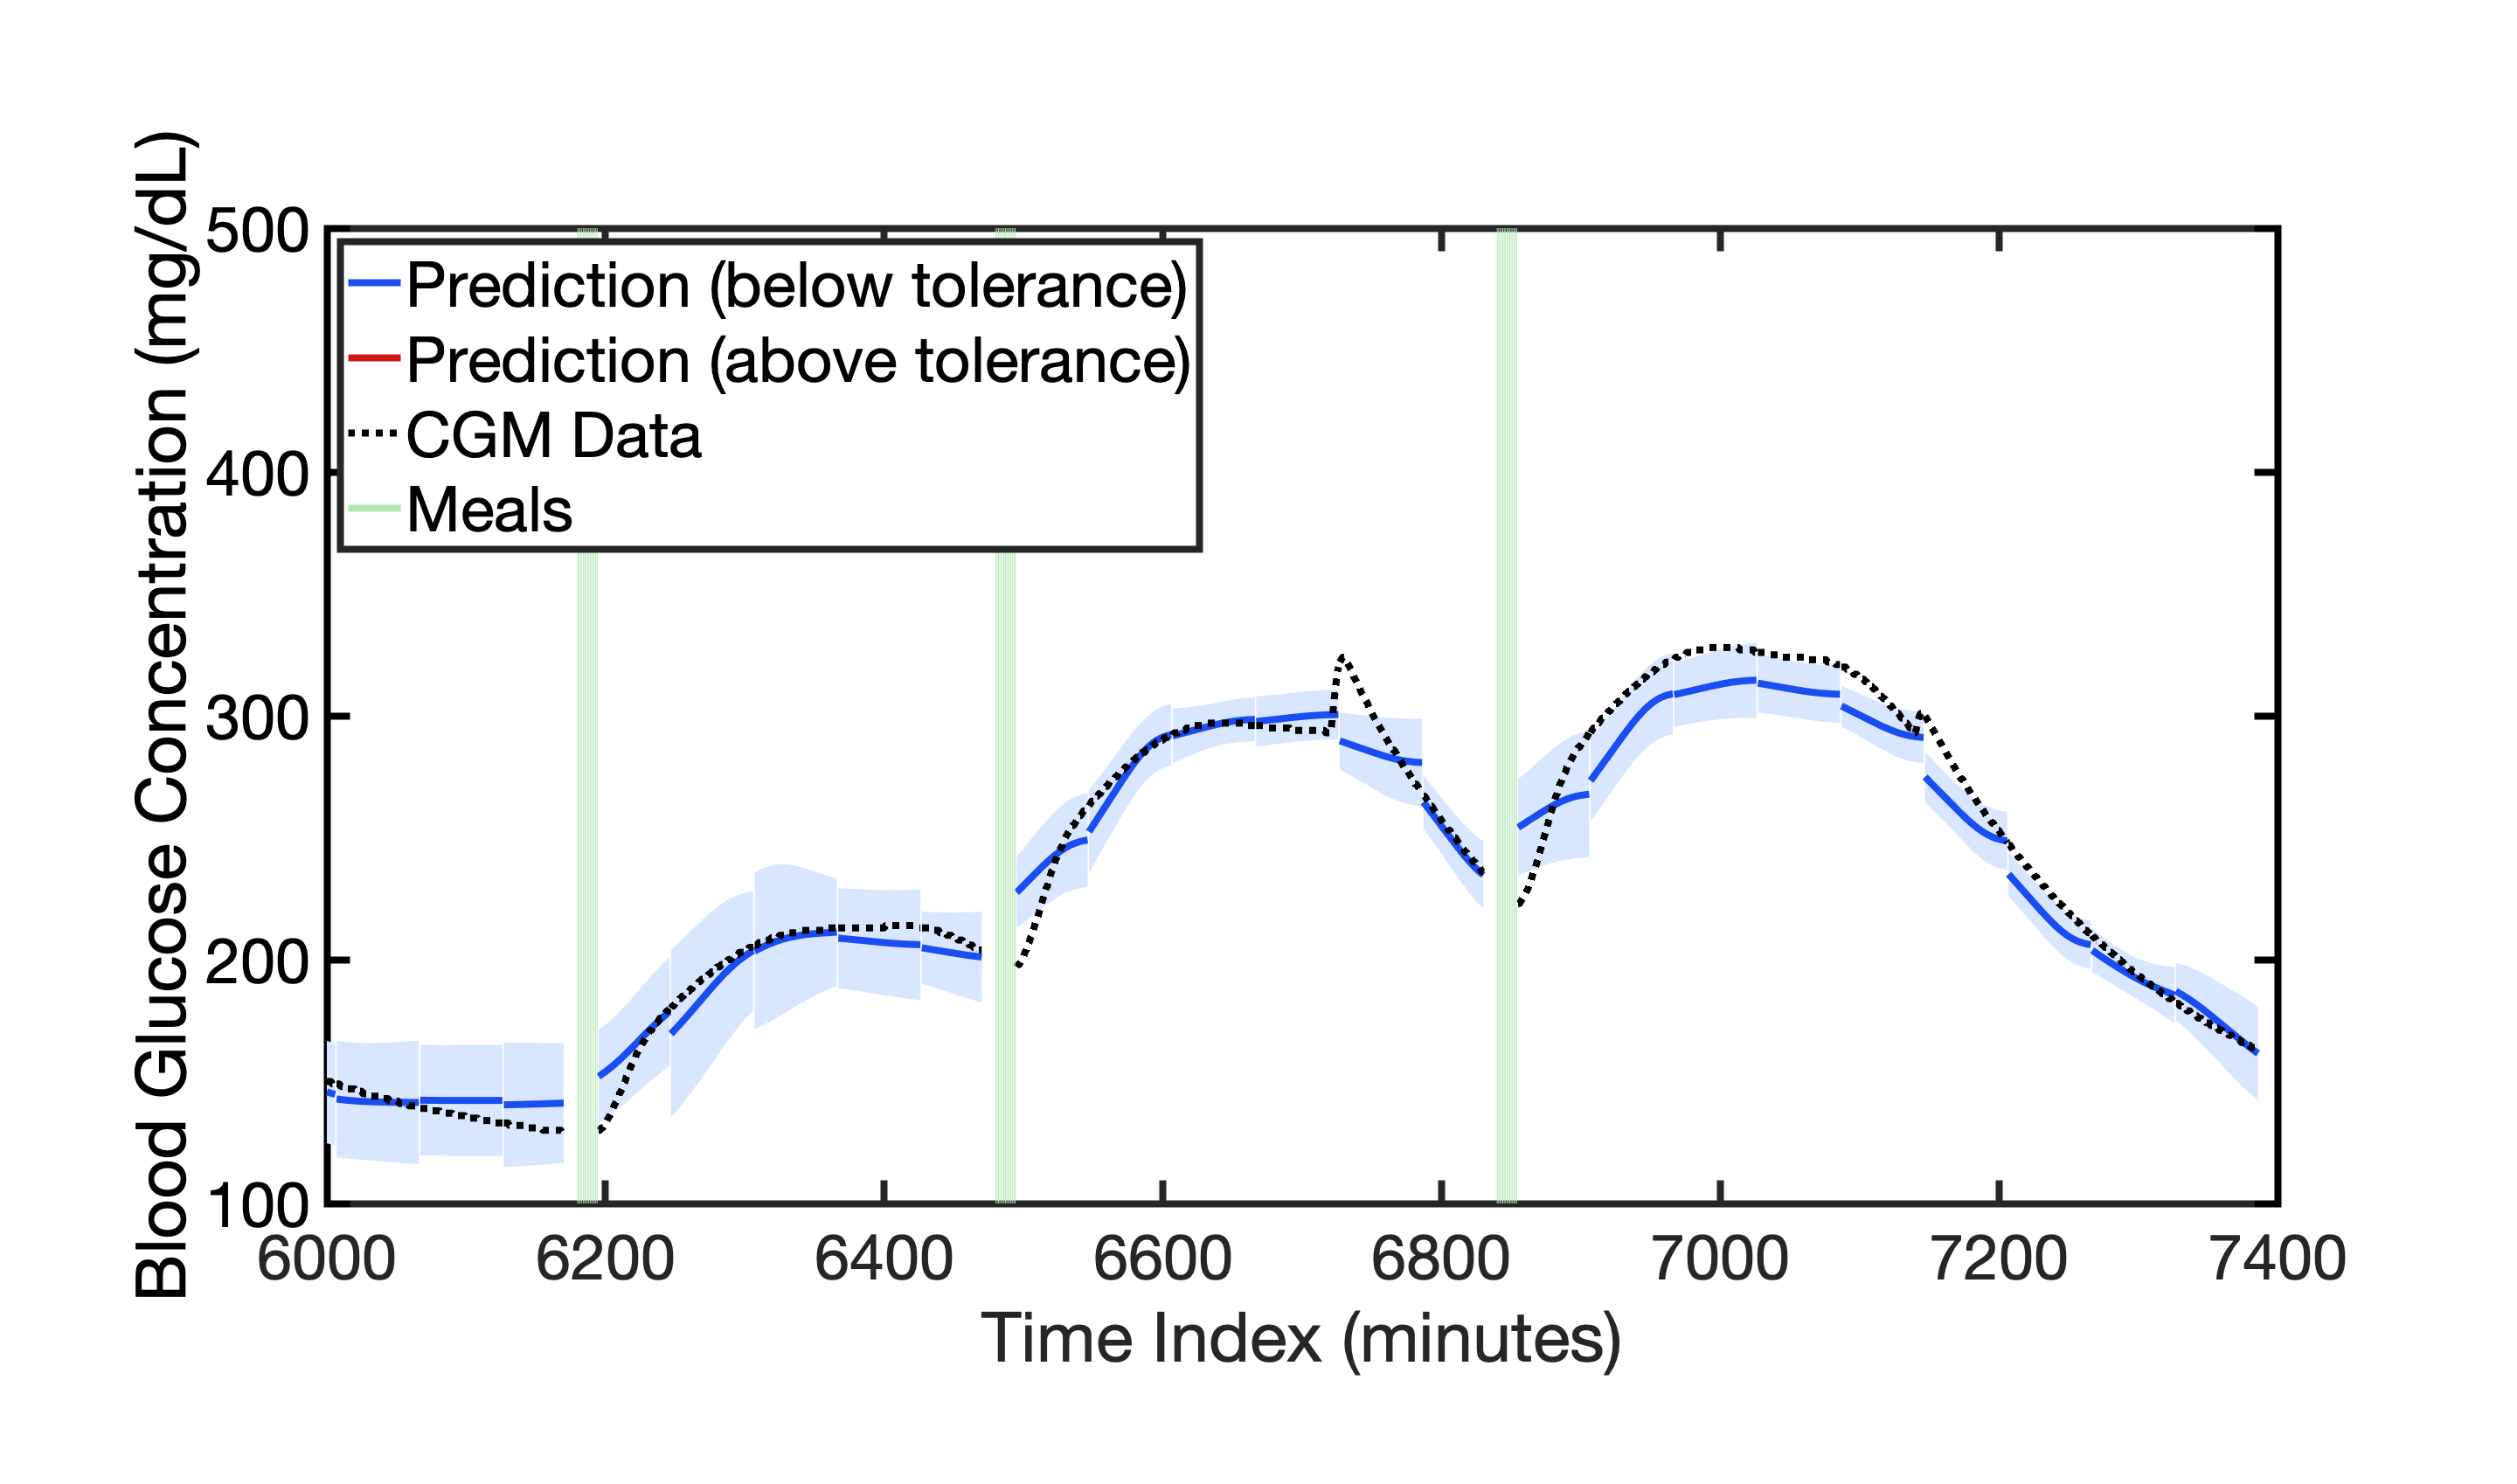
\includegraphics[width=0.43\linewidth]{Figures_manuscript/cat2_p3_c2.png}
  ~
  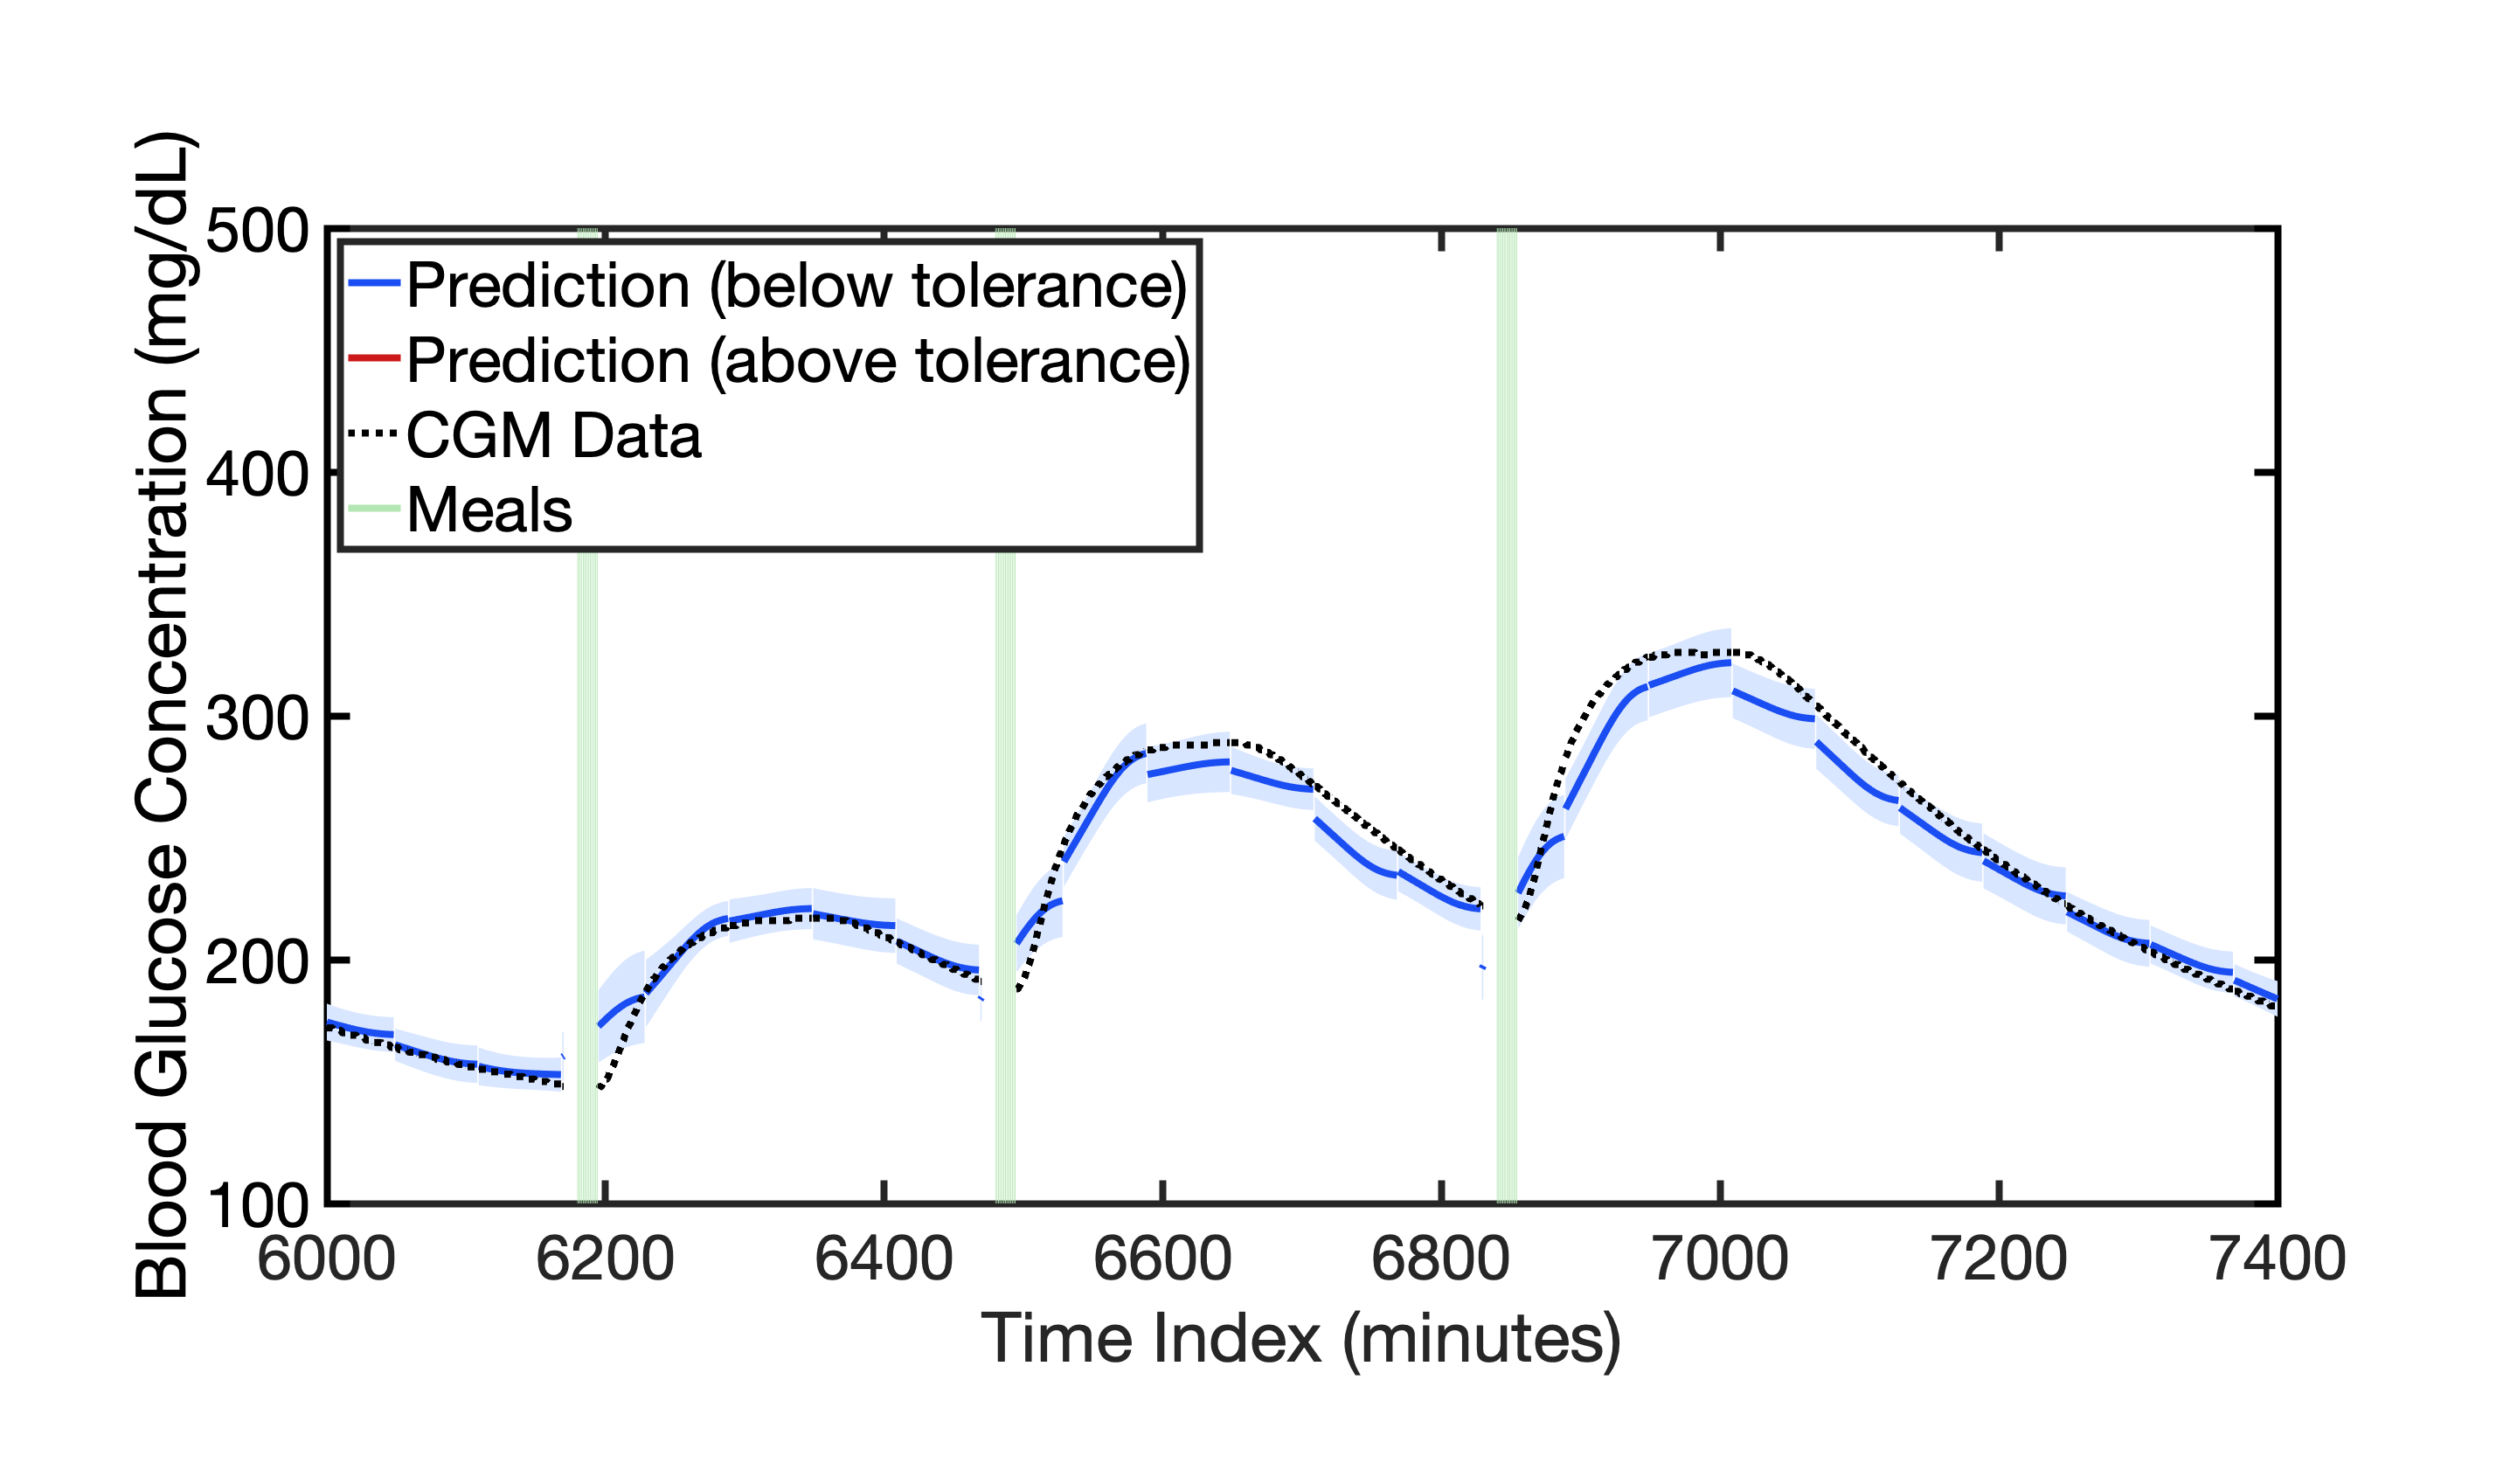
\includegraphics[width=0.43\linewidth]{Figures_manuscript/cat2_p4_c2.png}
  \vspace{-0.1in}
\\ (f)  \hspace{2.5in}  (g)
\vspace{-0.1in}
\caption{
Level~2 architecture ranking and validation outcomes. 
(a) Posterior plausibility \(\rho\) and MAP estimate of \(\sigma_{\text{noise}}\) as functions of model size (number of trainable parameters) for Level~2 architectures across validation folds (left to right: folds 1–5).
(b, c) Representative validation failures for most plausible architecture (\(Level_2Arch_2\)) on held-out patients 9 and 10 from Fold~1. Red segments indicate one-hour prediction windows that violate the acceptance criterion \(\mathrm{NLPD} \leq Tol\).
(d--g) Validation results for the EVIDENT-selected architecture (\(Level_2Arch_4\)) across multiple folds and held-out patients: (d,e) patients 1--2 and (f,g) patients 3--4. The one-hour forecasts of (\(Level_2Arch_4\)) passes all the validation tests, demonstrating EVIDENT identified trustworthy predictor.
}
\label{fig:level2_plausibility_failure_sucess}
\end{figure}


%-- Level 2: validation
The top-ranked architectures in each fold are subsequently evaluated on the held-out subjects using the validation protocol. Although Level~2 architectures exhibit improved predictive performance relative to Level~1, most candidates still fail the validation criterion by violating the NLPD tolerance in a subset of one-hour prediction windows (representative failure cases are shown in Figure~\ref{fig:level2_plausibility_failure_sucess}(b,c)).
EVIDENT, however, identifies a single architecture, \(Level_2Arch_4\), that satisfies the validation criterion across all folds and held-out subjects. As shown in Figure~\ref{fig:level2_plausibility_failure_sucess}(d--g), this model produces consistent one-hour forecasts that remain within the prescribed tolerance across all validation windows. This architecture is therefore selected as the trustworthy predictor.




% -- Level 2: BMA
%
\begin{figure}[!ht]
\centering
  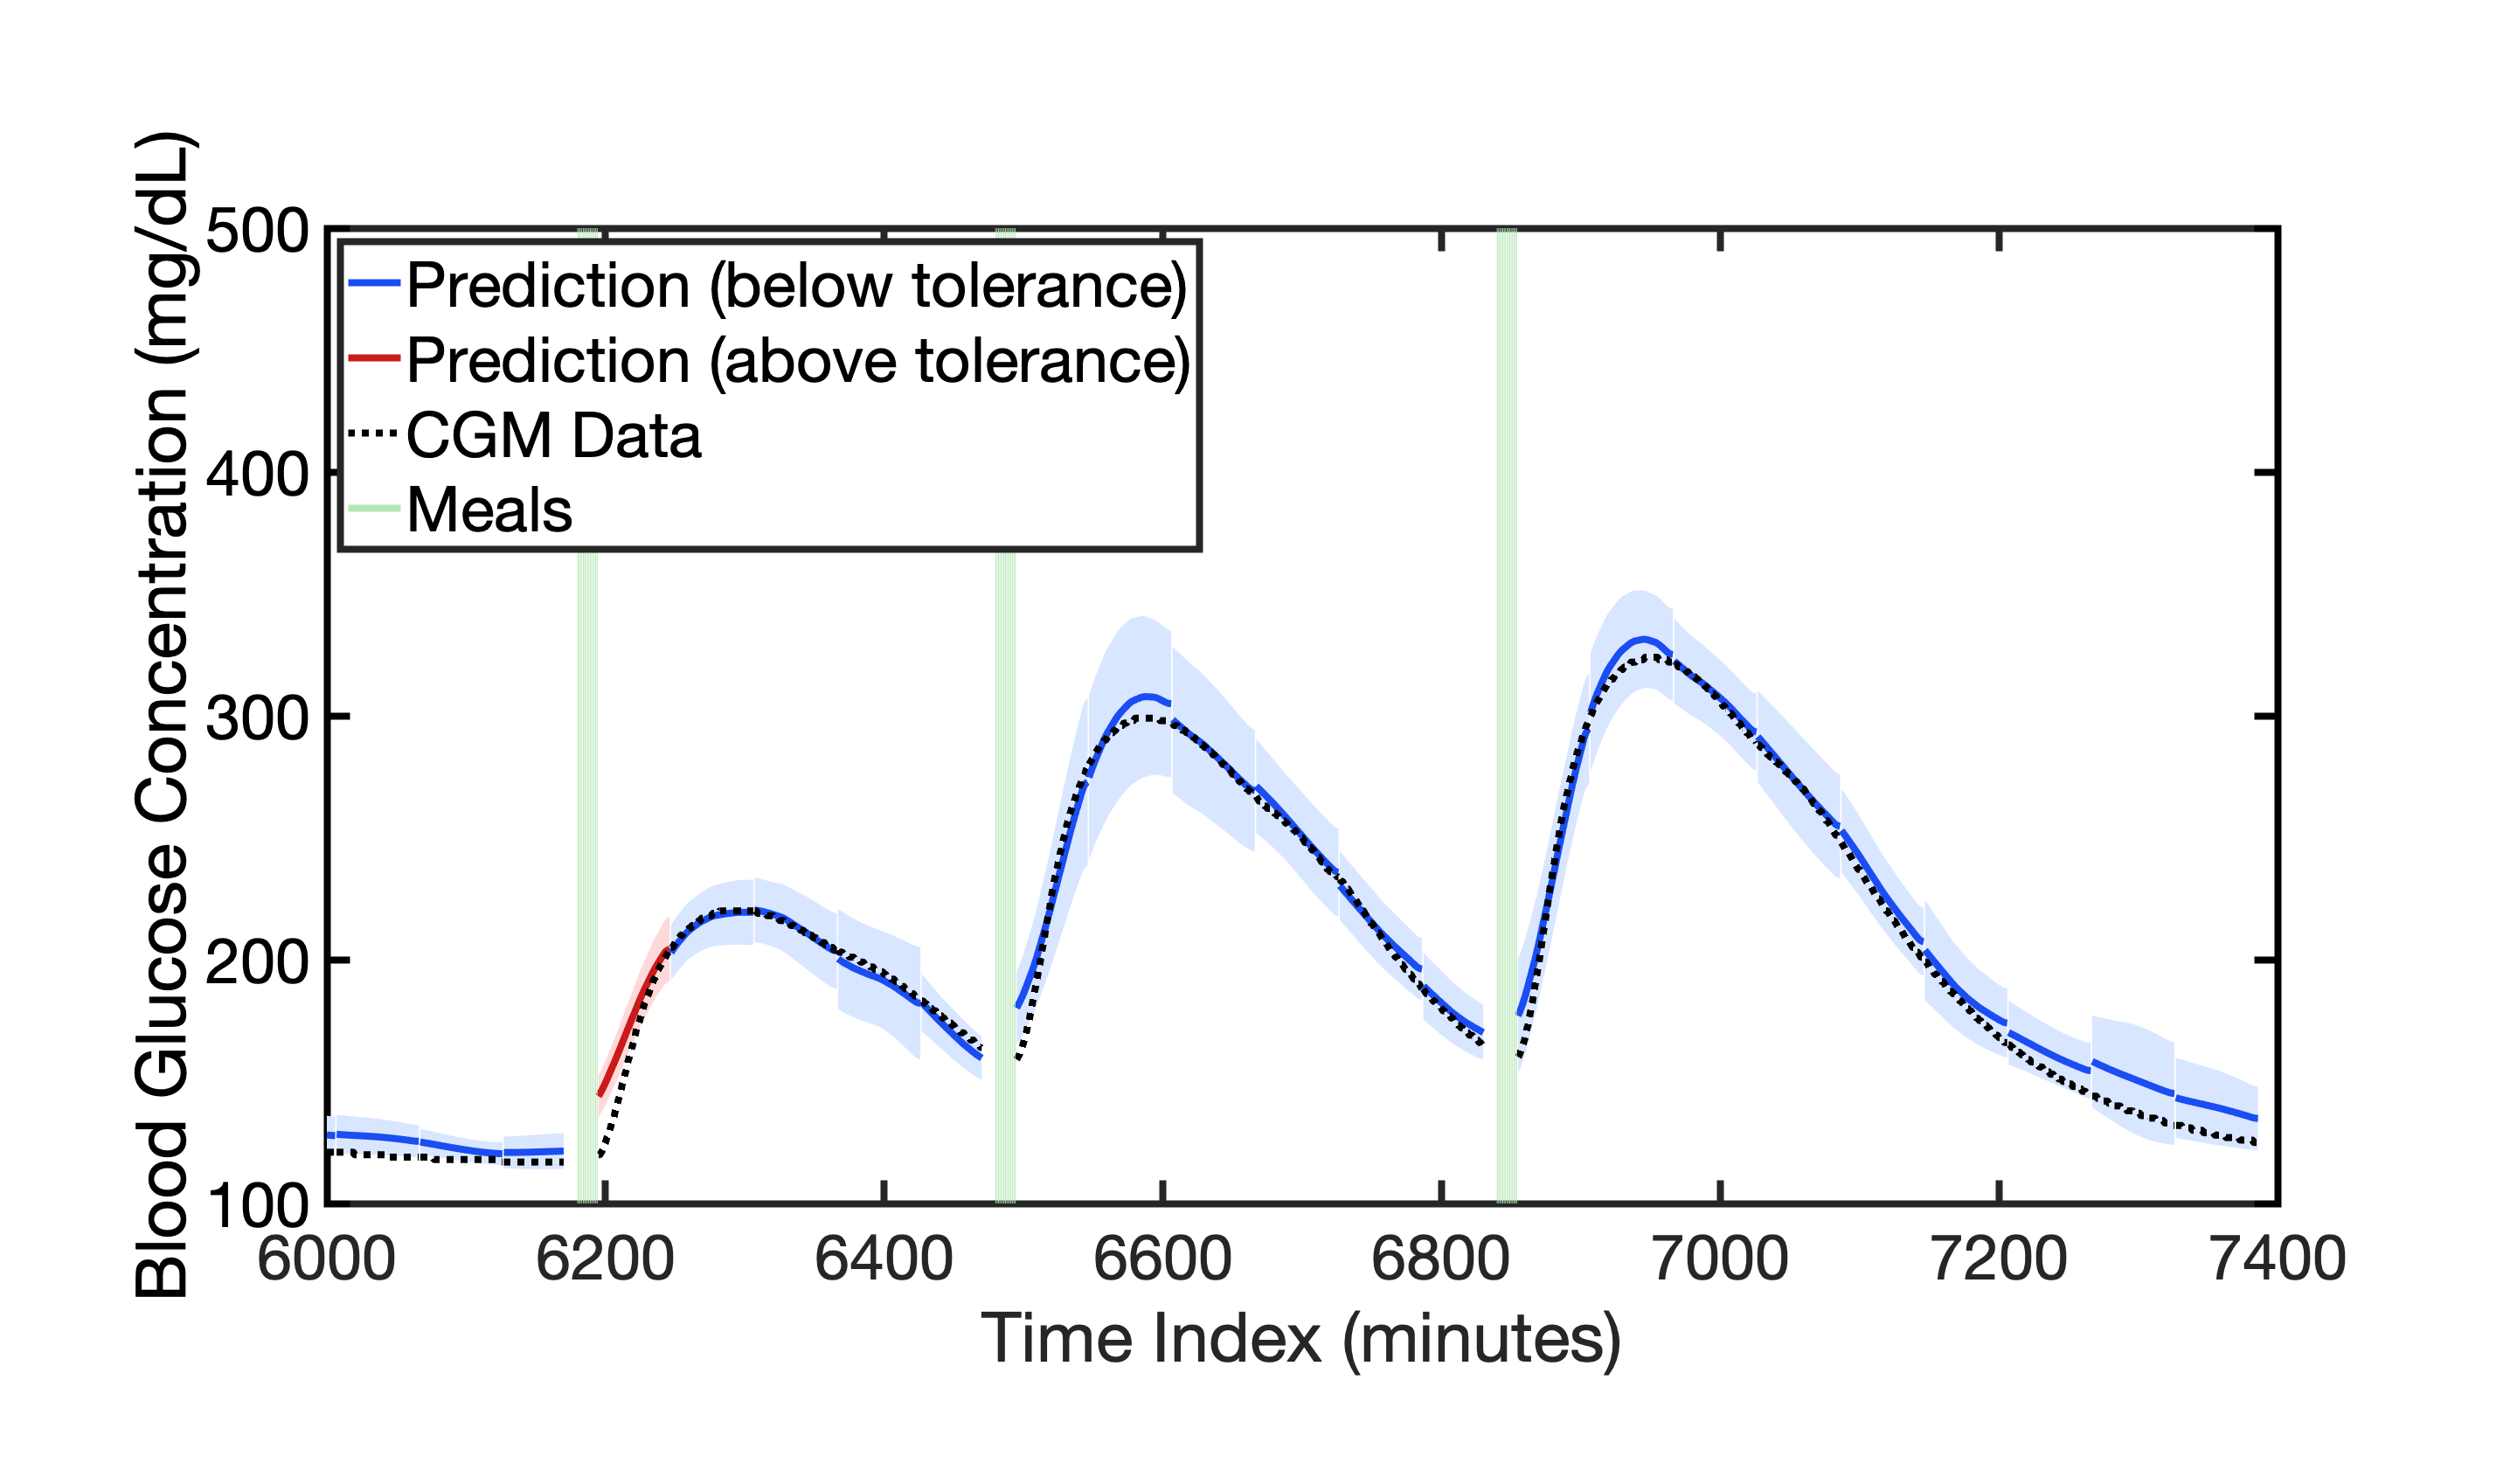
\includegraphics[width=0.45\linewidth]{Figures_manuscript/cat2_p6_c2.png}
    ~
  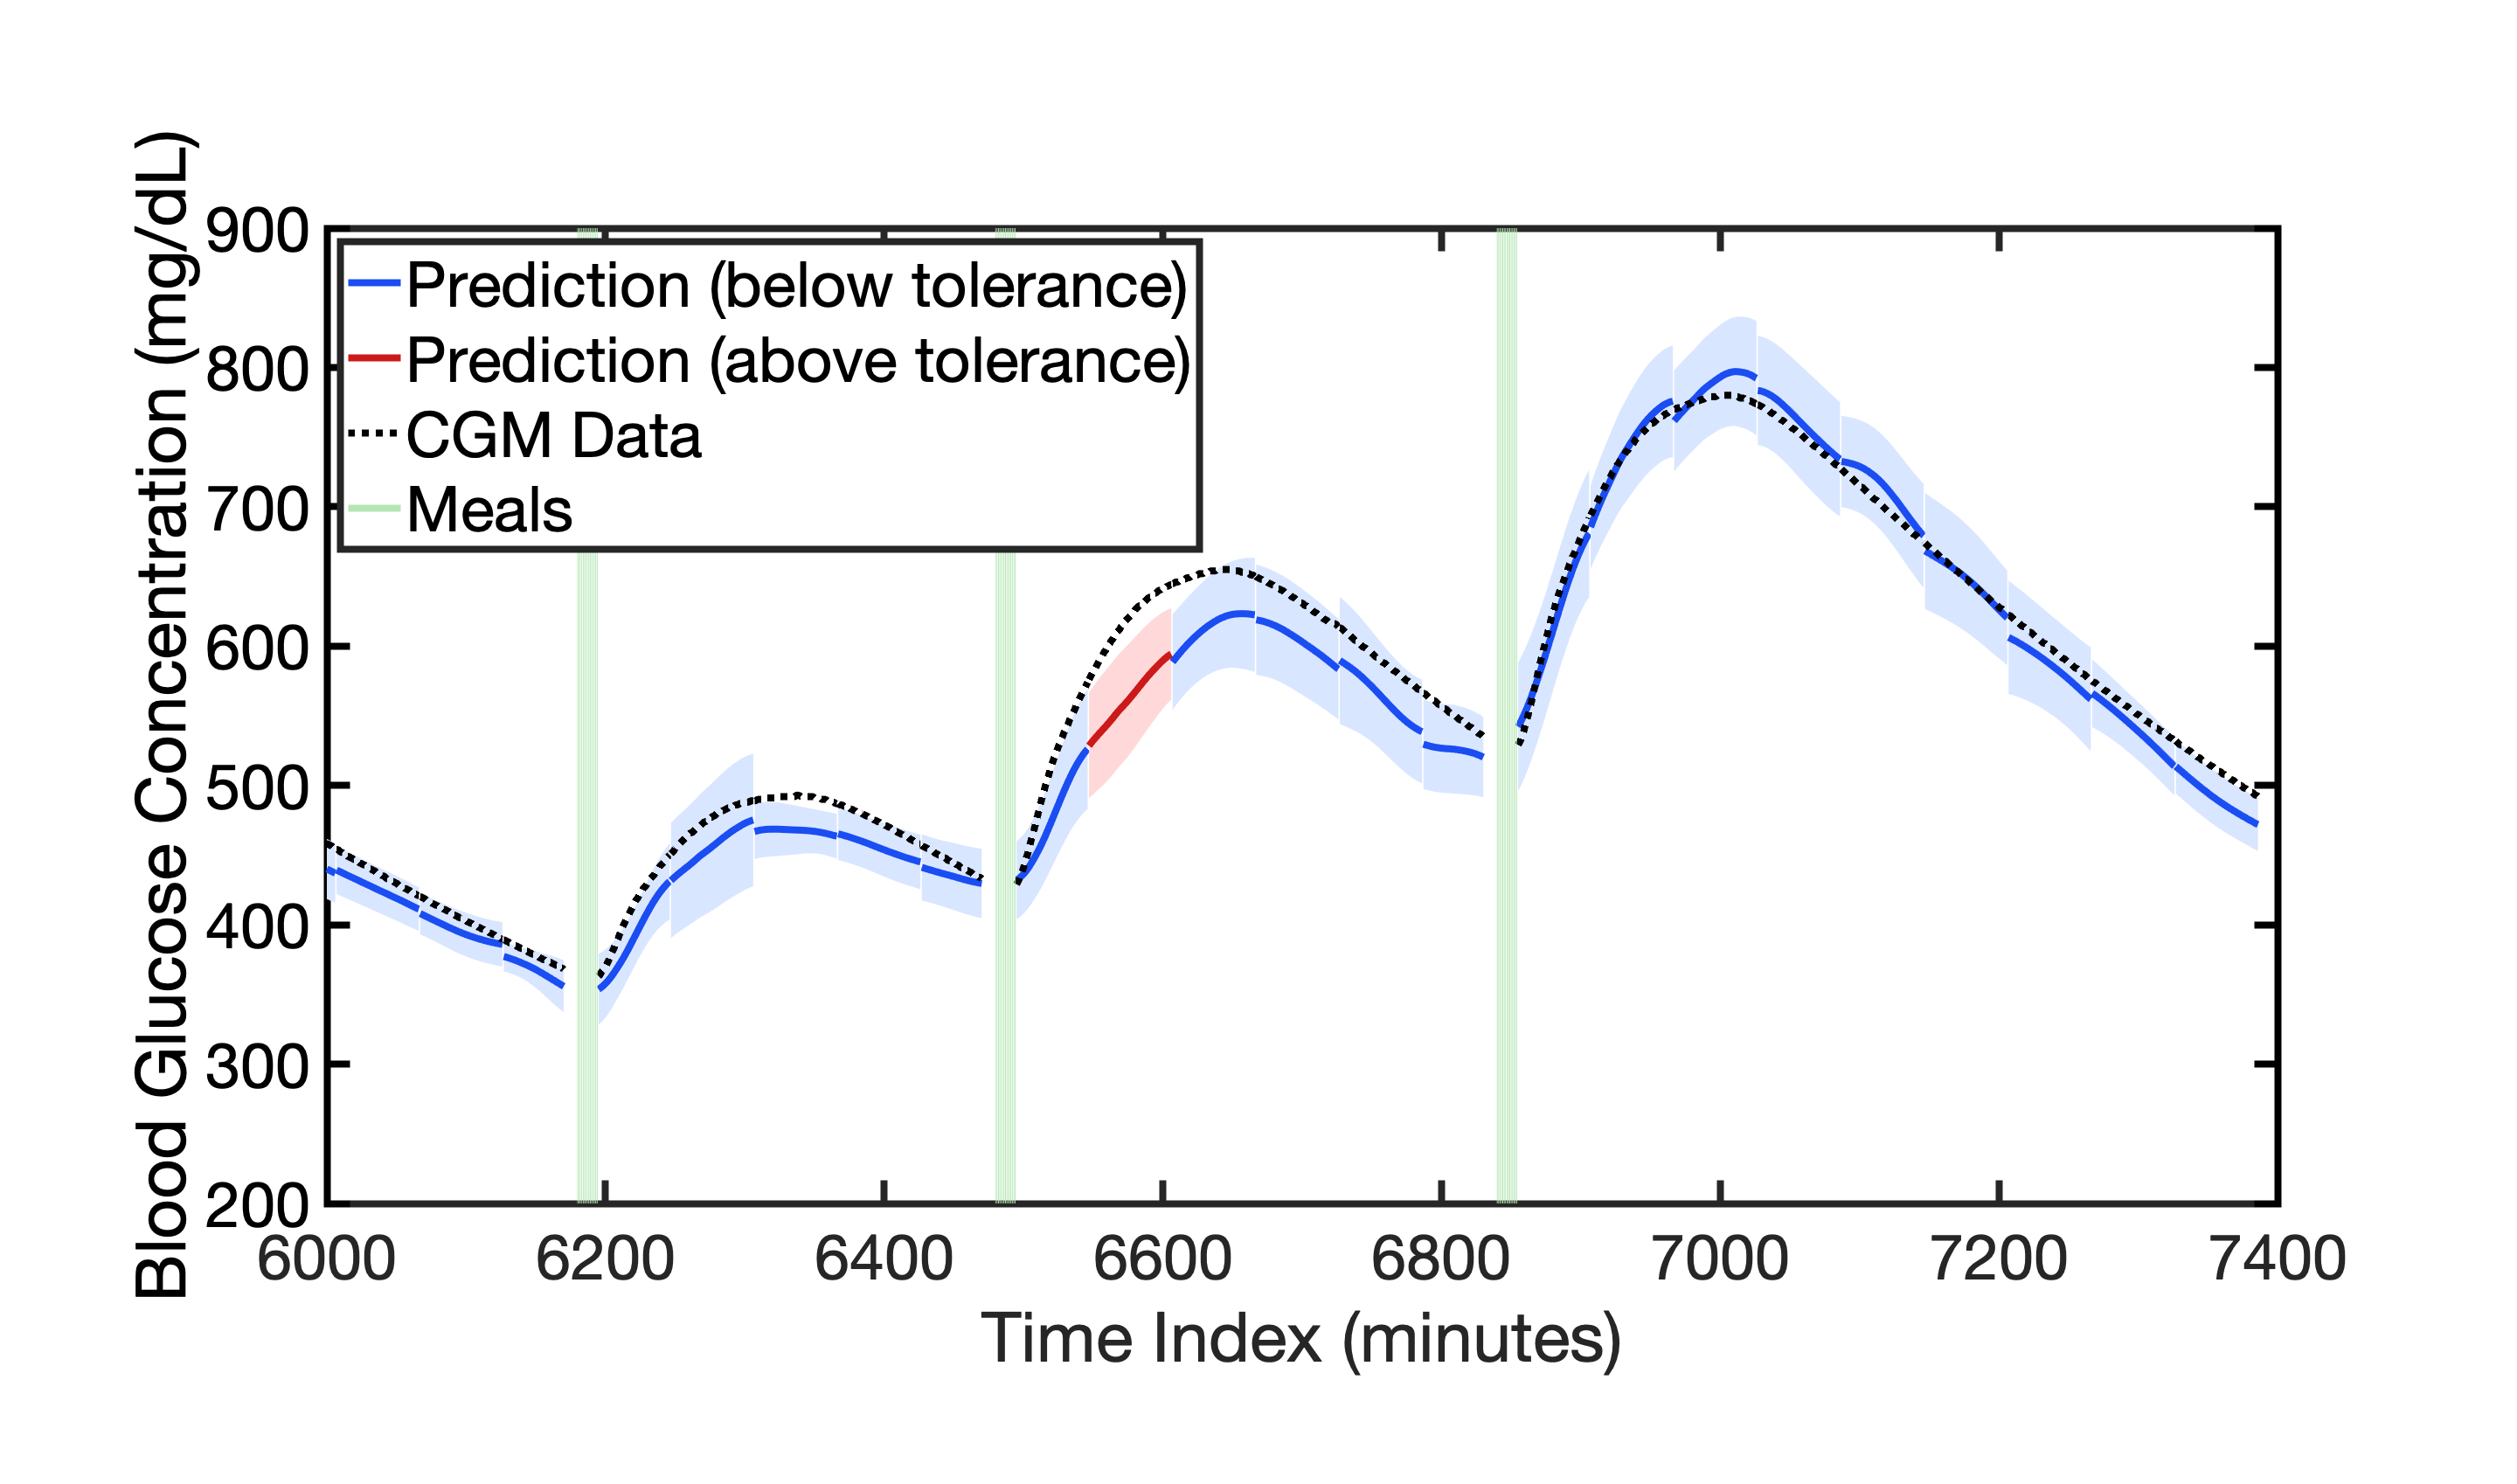
\includegraphics[width=0.45\linewidth]{Figures_manuscript/cat2_p7_c2.png}
  \vspace{-0.1in}
  \\ (a) \hspace{2.5in} (b) \\
  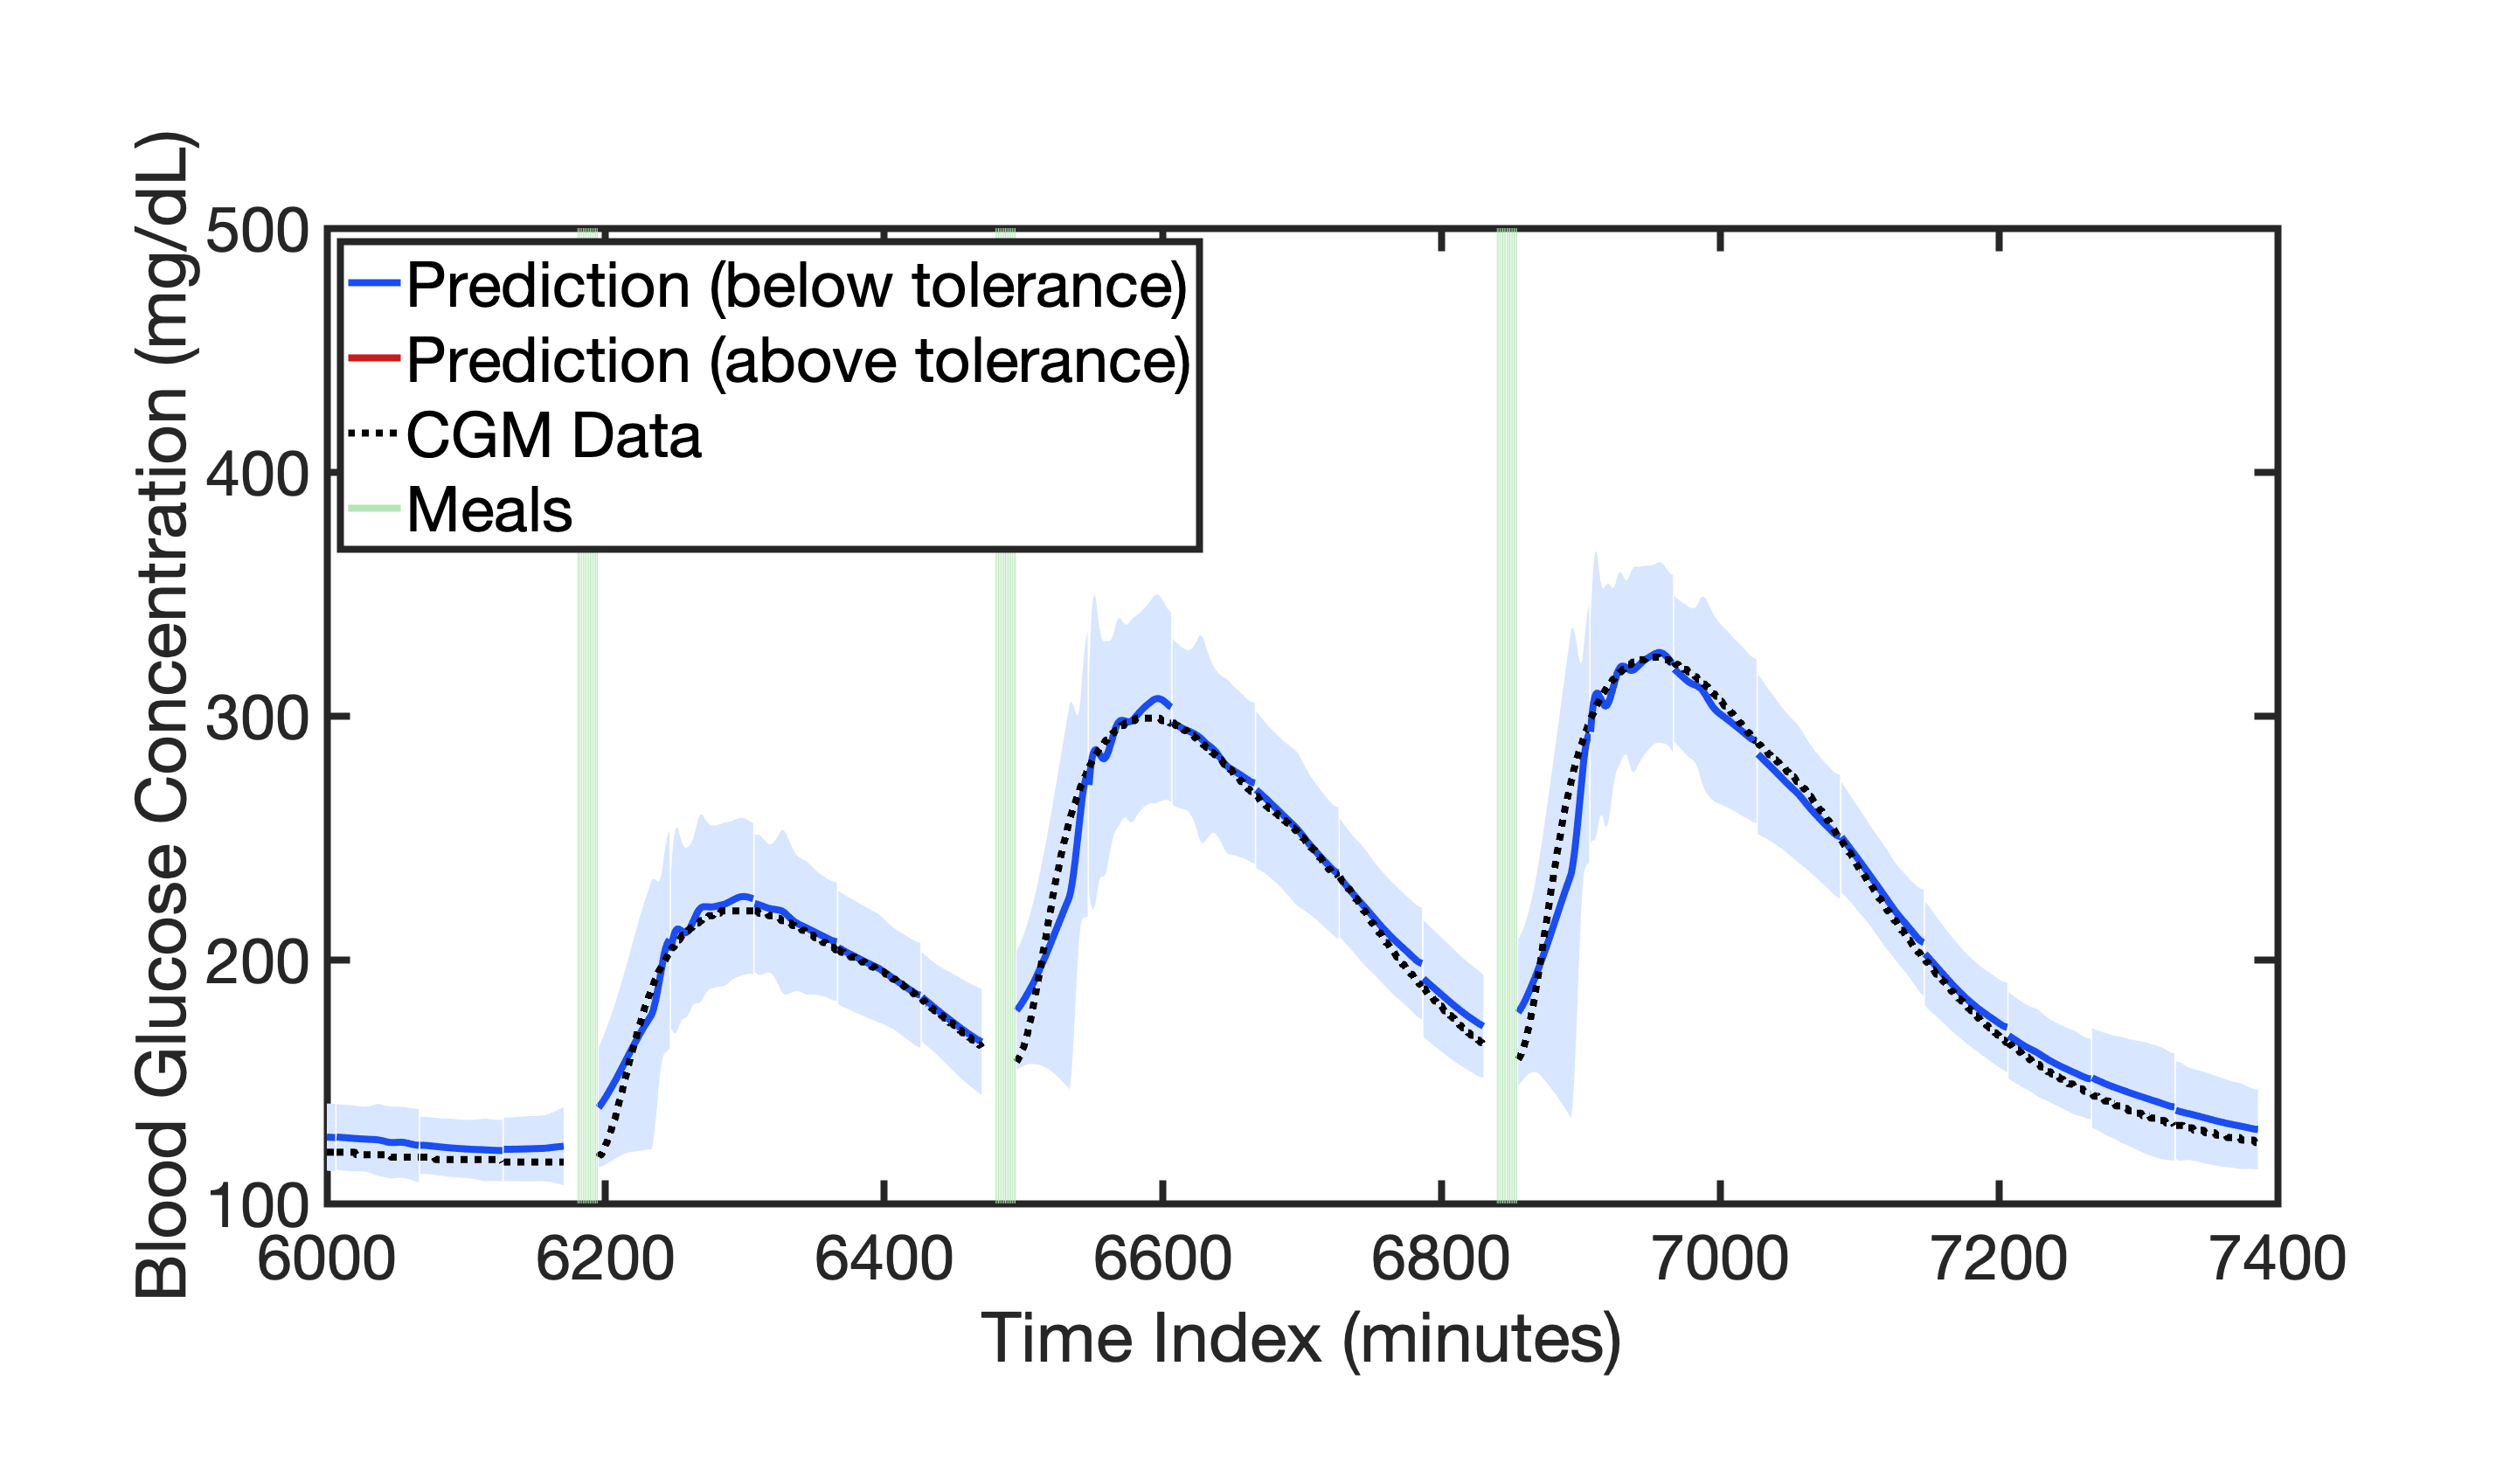
\includegraphics[width=0.45\linewidth]{Figures_manuscript/cat2_p6_bma.png}
  ~
  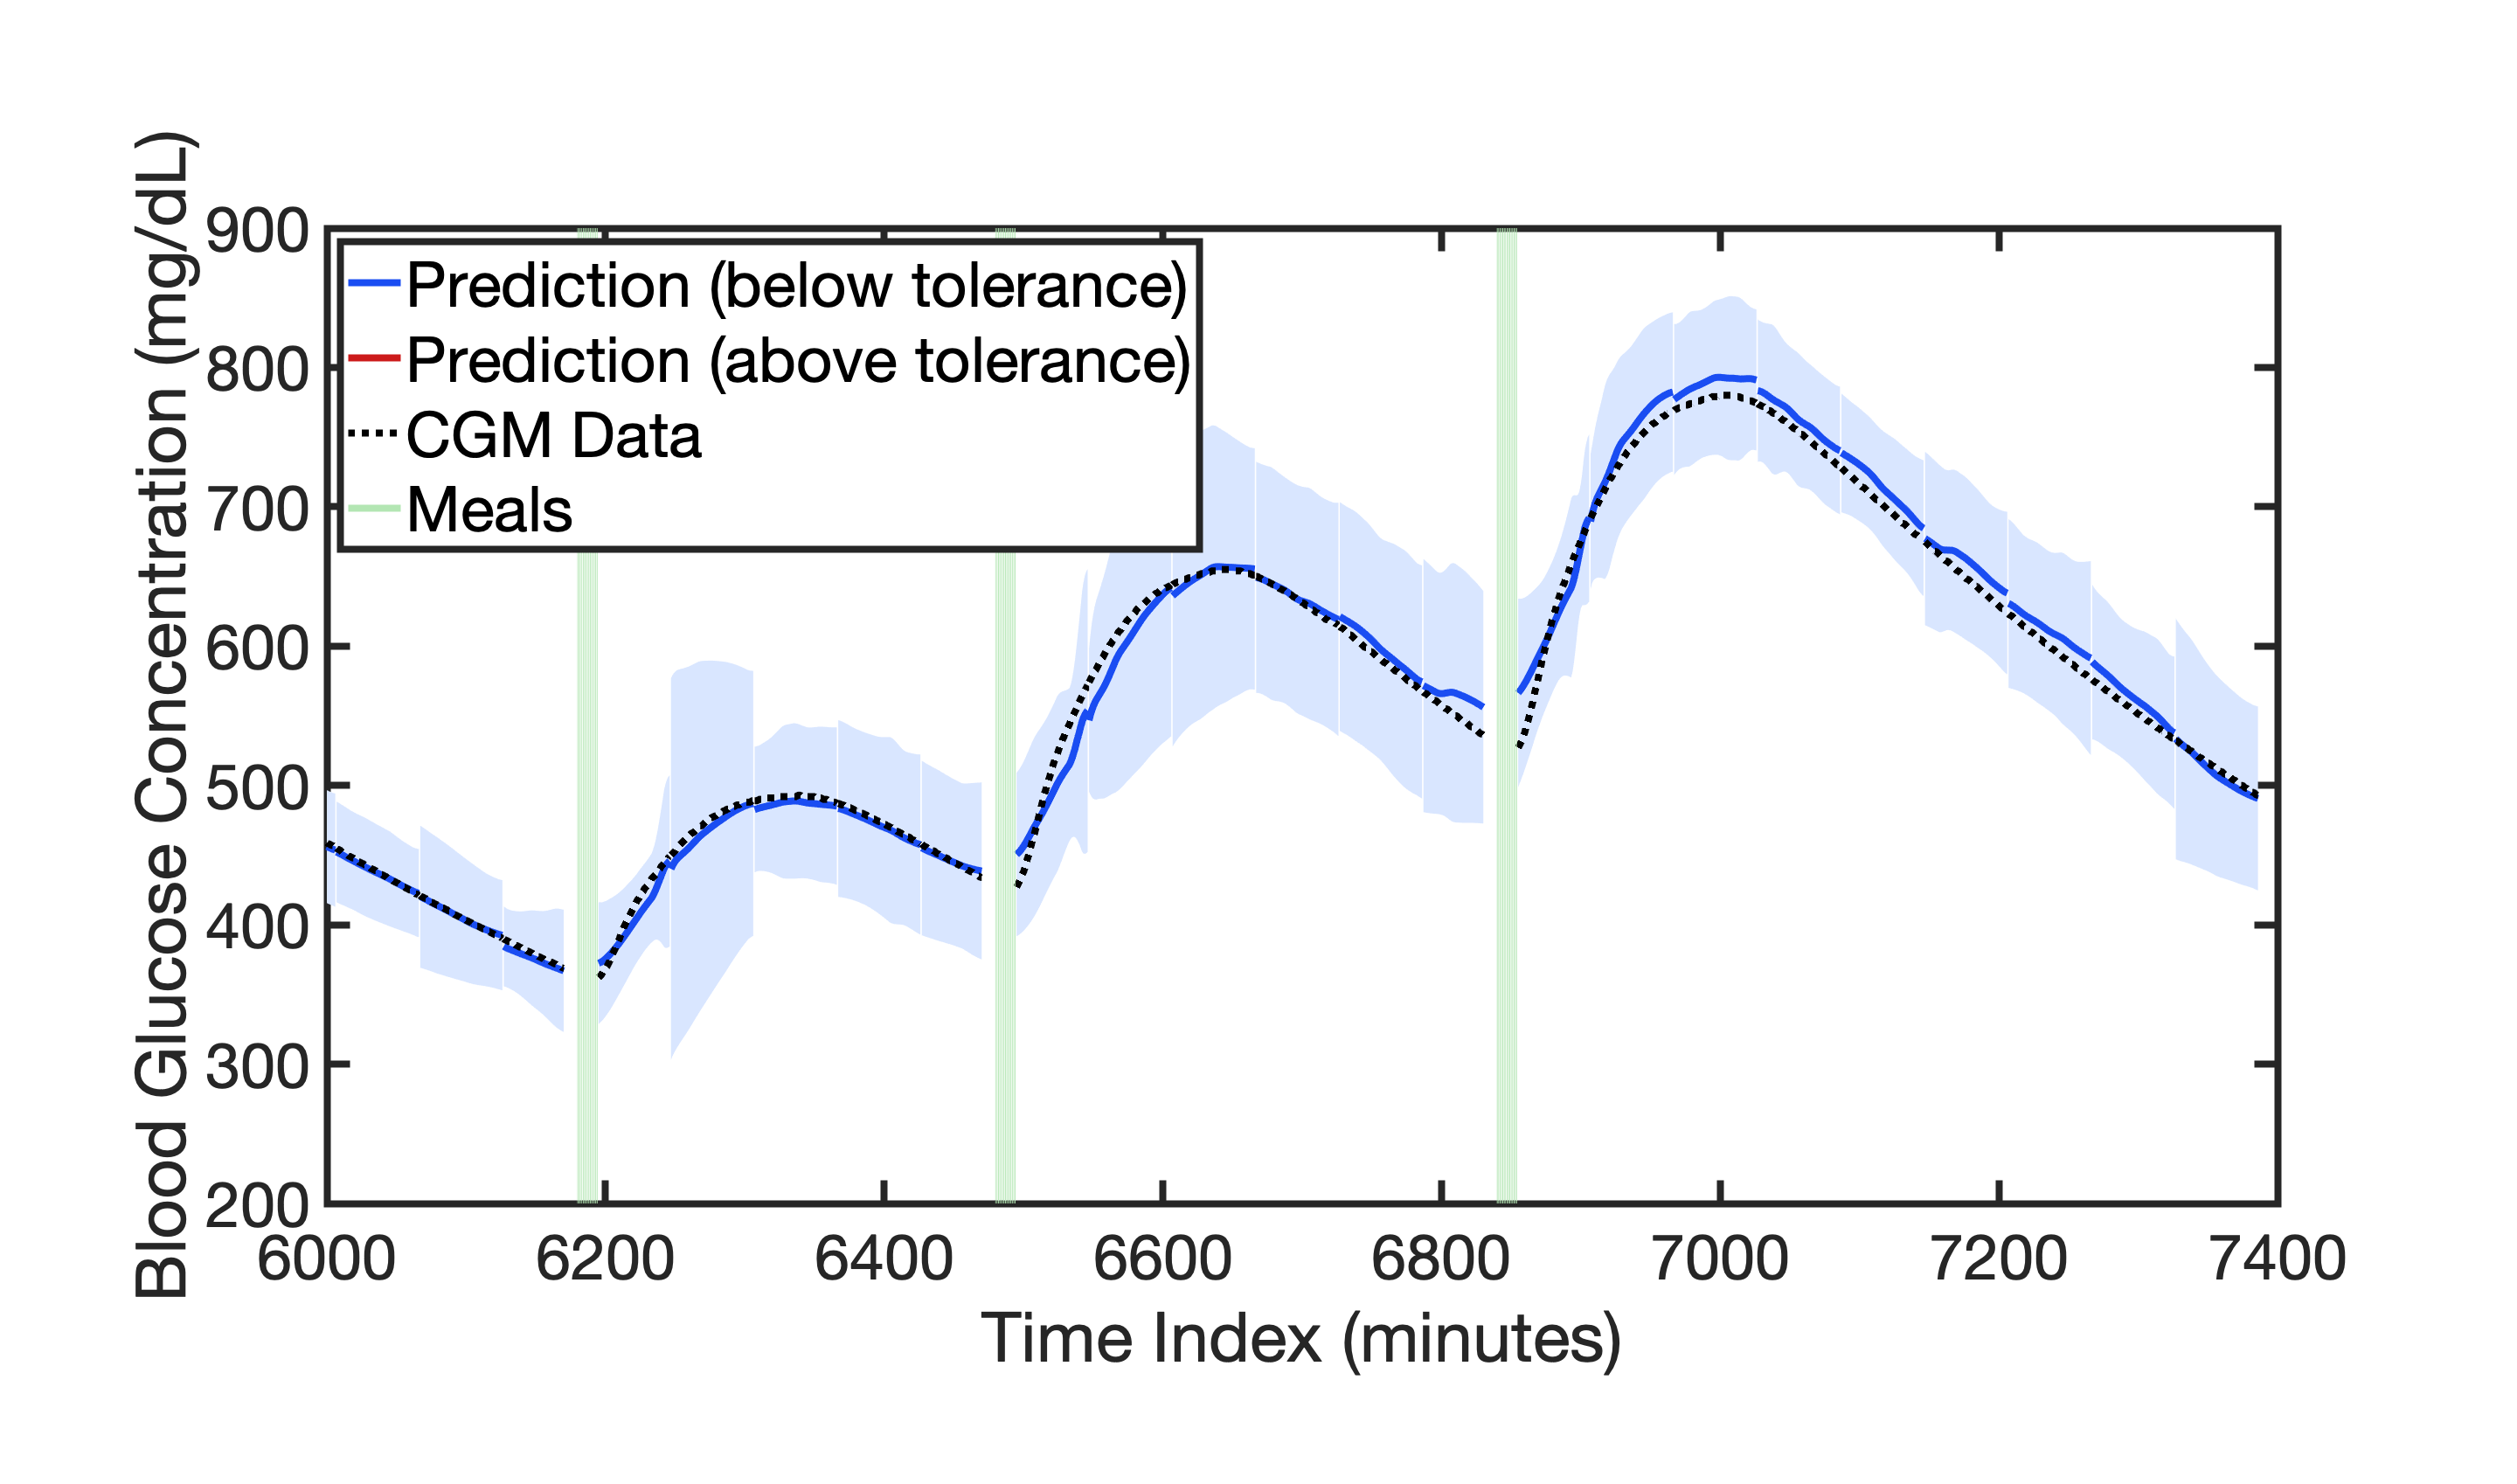
\includegraphics[width=0.45\linewidth]{Figures_manuscript/cat2_p7_bma.png}
  \vspace{-0.1in}
  \\ (c) \hspace{2.5in} (d)
  \vspace{-0.1in}
\caption{Comparison of single-architecture and plausibility-weighted ensemble predictions for representative Level~2 candidates in fold~2. 
(a–-b) Predictions from a single architecture ($Level_2Arch_7$) for Patients 6–7 in fold~2, and 
(c–-d) corresponding ensemble predictions from all architectures in Level~2.
Red segments indicate one-hour prediction windows that violates the acceptance criterion $NLPD \leq Tol$.}
\label{fig:bma}
\end{figure}
%
In addition to single-architecture selection, EVIDENT also supports a plausibility-weighted ensemble predictor when multiple architectures remain competitive. To assess this, we compare the predictions of the most plausible architecture with the ensemble prediction defined in \eqref{eq:bma} over all Level~2 architectures for fold~2 (Figure~\ref{fig:bma}).
The ensemble achieves improved predictive accuracy and lower NLPD relative to individual architectures, while producing wider uncertainty bands due to aggregation across models. This behavior reflects an ensemble effect, where different architectures capture complementary temporal patterns and their combination mitigates individual model deficiencies. These results indicate that, although a single architecture can satisfy the validation criterion, the plausibility-weighted ensemble provides a mechanism for improving predictive performance while capturing model uncertainty in the presence of multiple candidates.






\paragraph{Capacity level 3 ($l=3$)}
Level~3 contains higher-capacity architectures ($10^5$–$4\times10^5$ parameters). Despite their increased representational capacity, these models do not improve validation performance and frequently violate the NLPD criterion across multiple prediction windows (Figure~\ref{fig:pred_cat3}).
The additional parameters at this level are not sufficiently learned by the available data, leading to degraded generalization under inter-patient variability. In contrast to Level~2, where intermediate-capacity architectures satisfy the validation criterion, increasing capacity beyond this regime yields no consistent improvement and introduces  prediction errors.


\begin{figure}[!ht]
\centering
  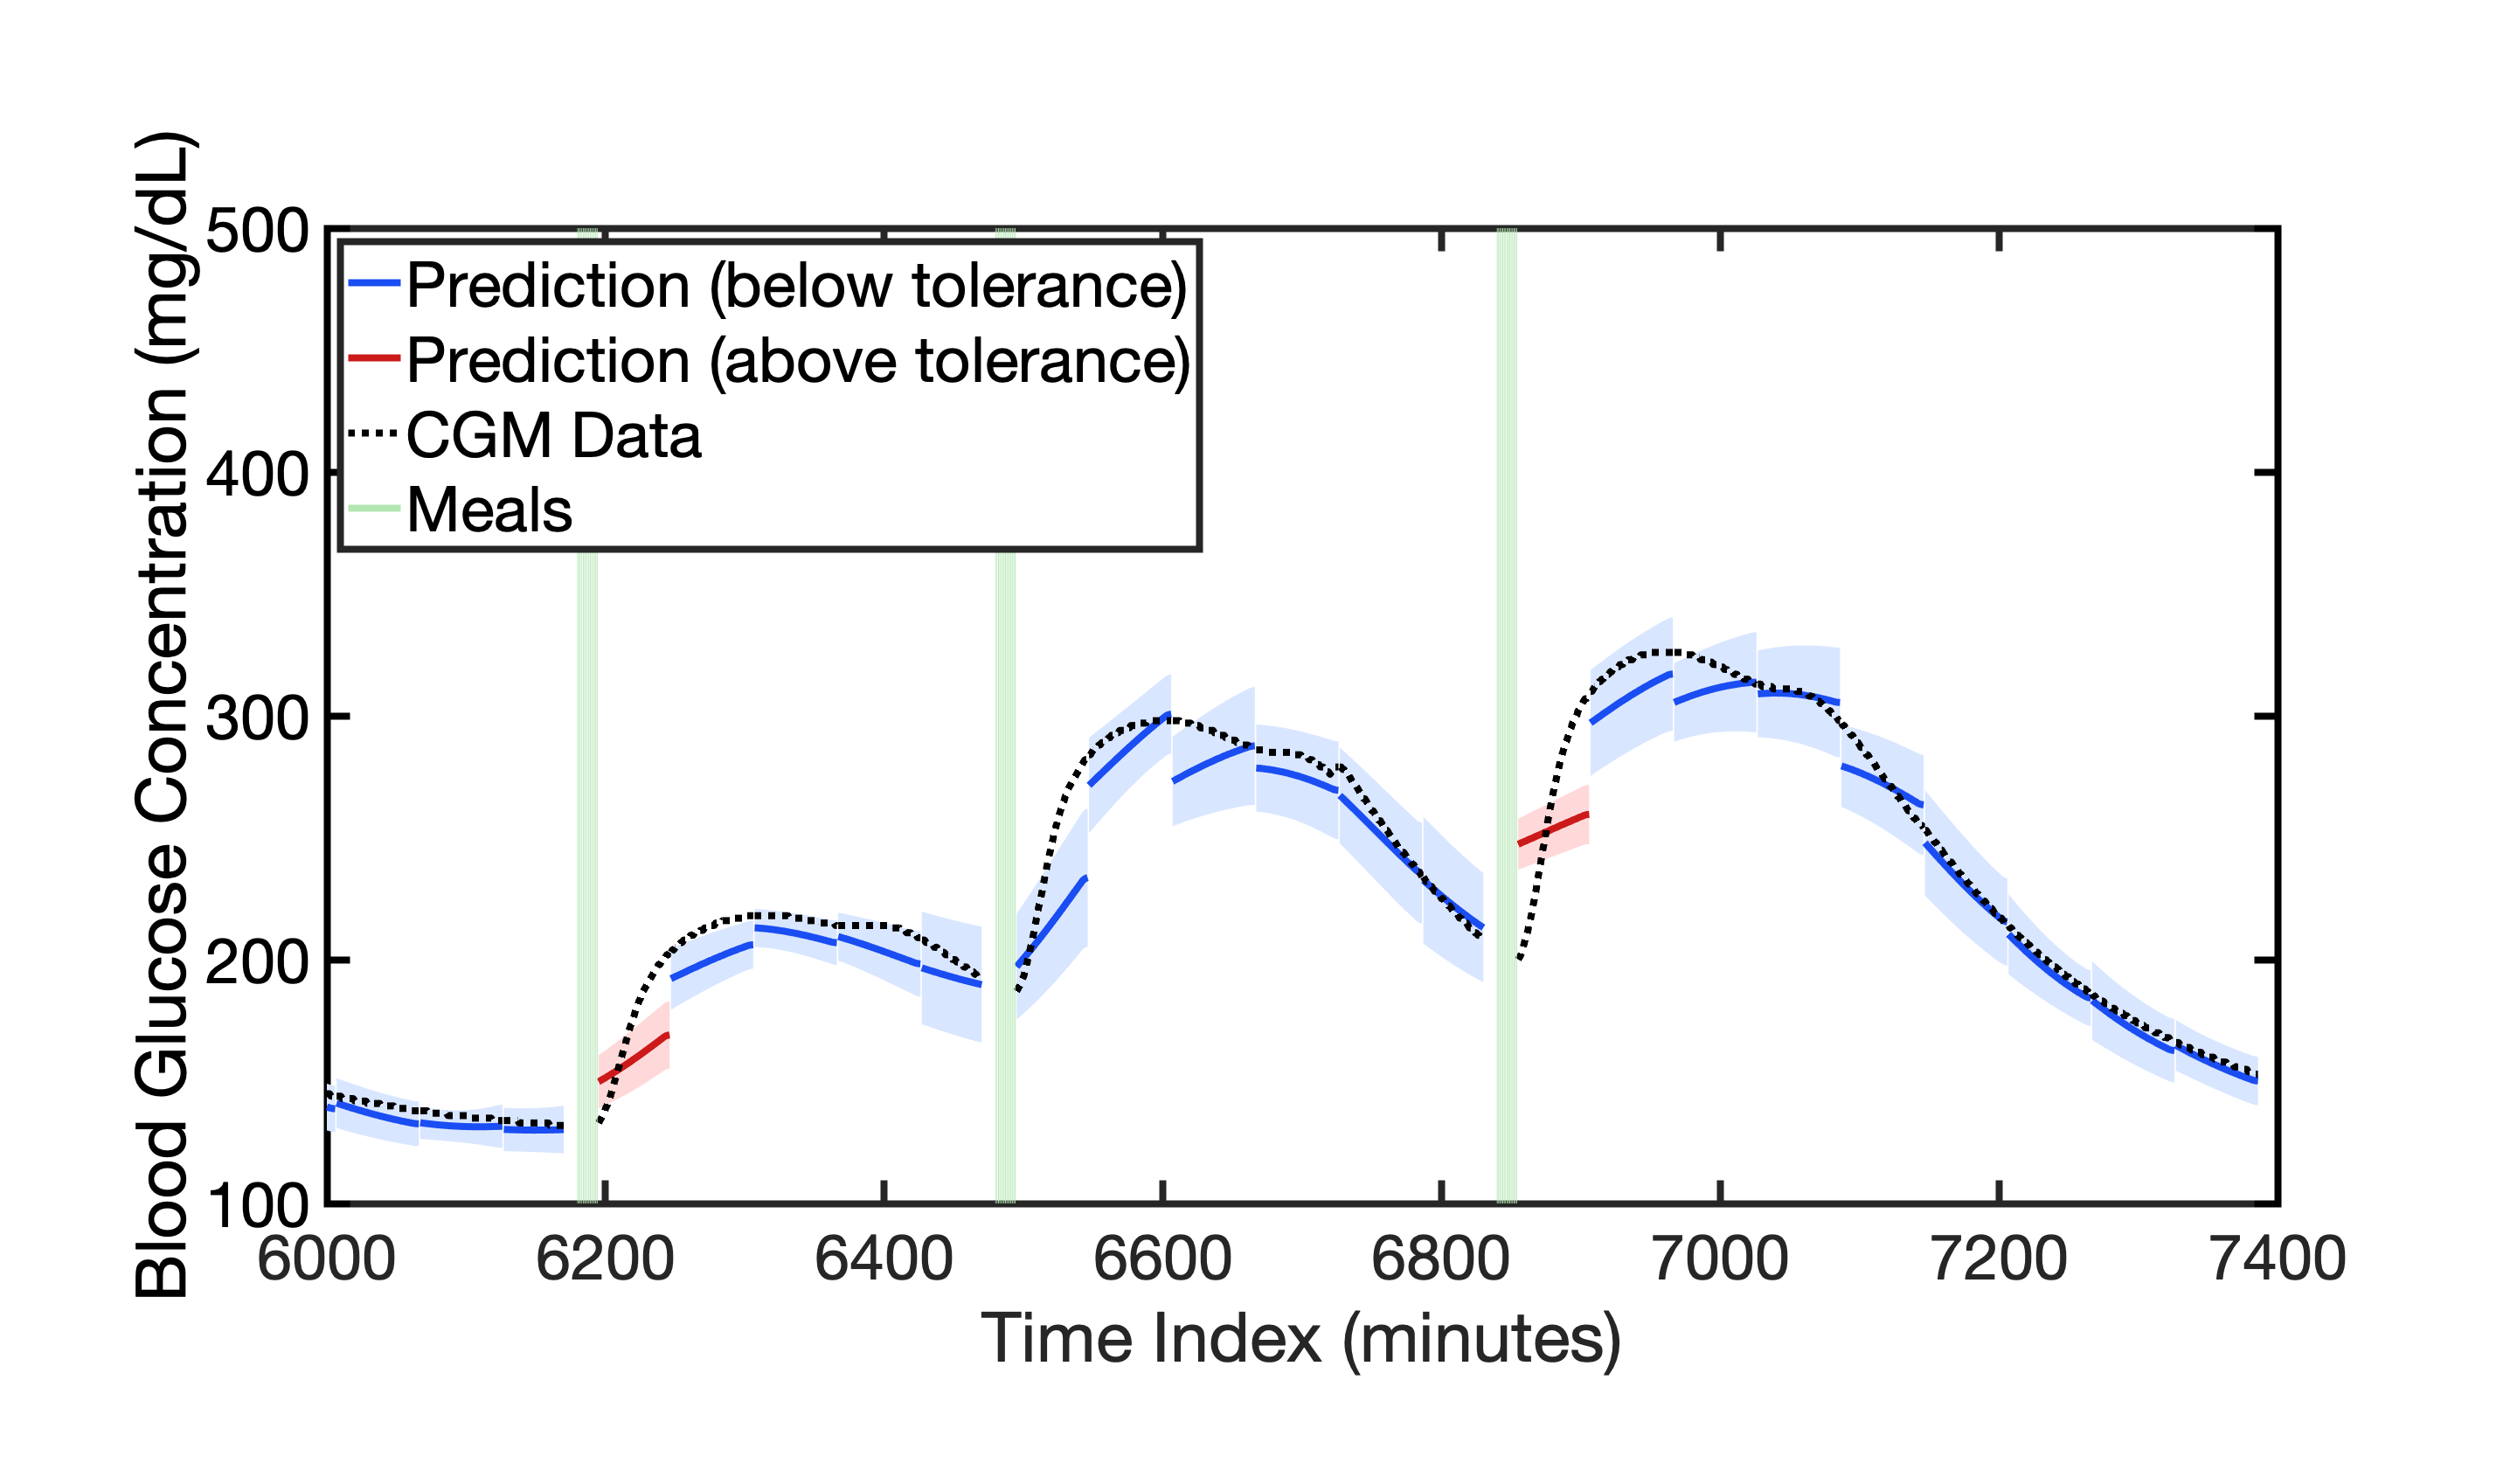
\includegraphics[width=0.45\linewidth]{Figures_manuscript/cat3_p1_c3.png}
  ~
  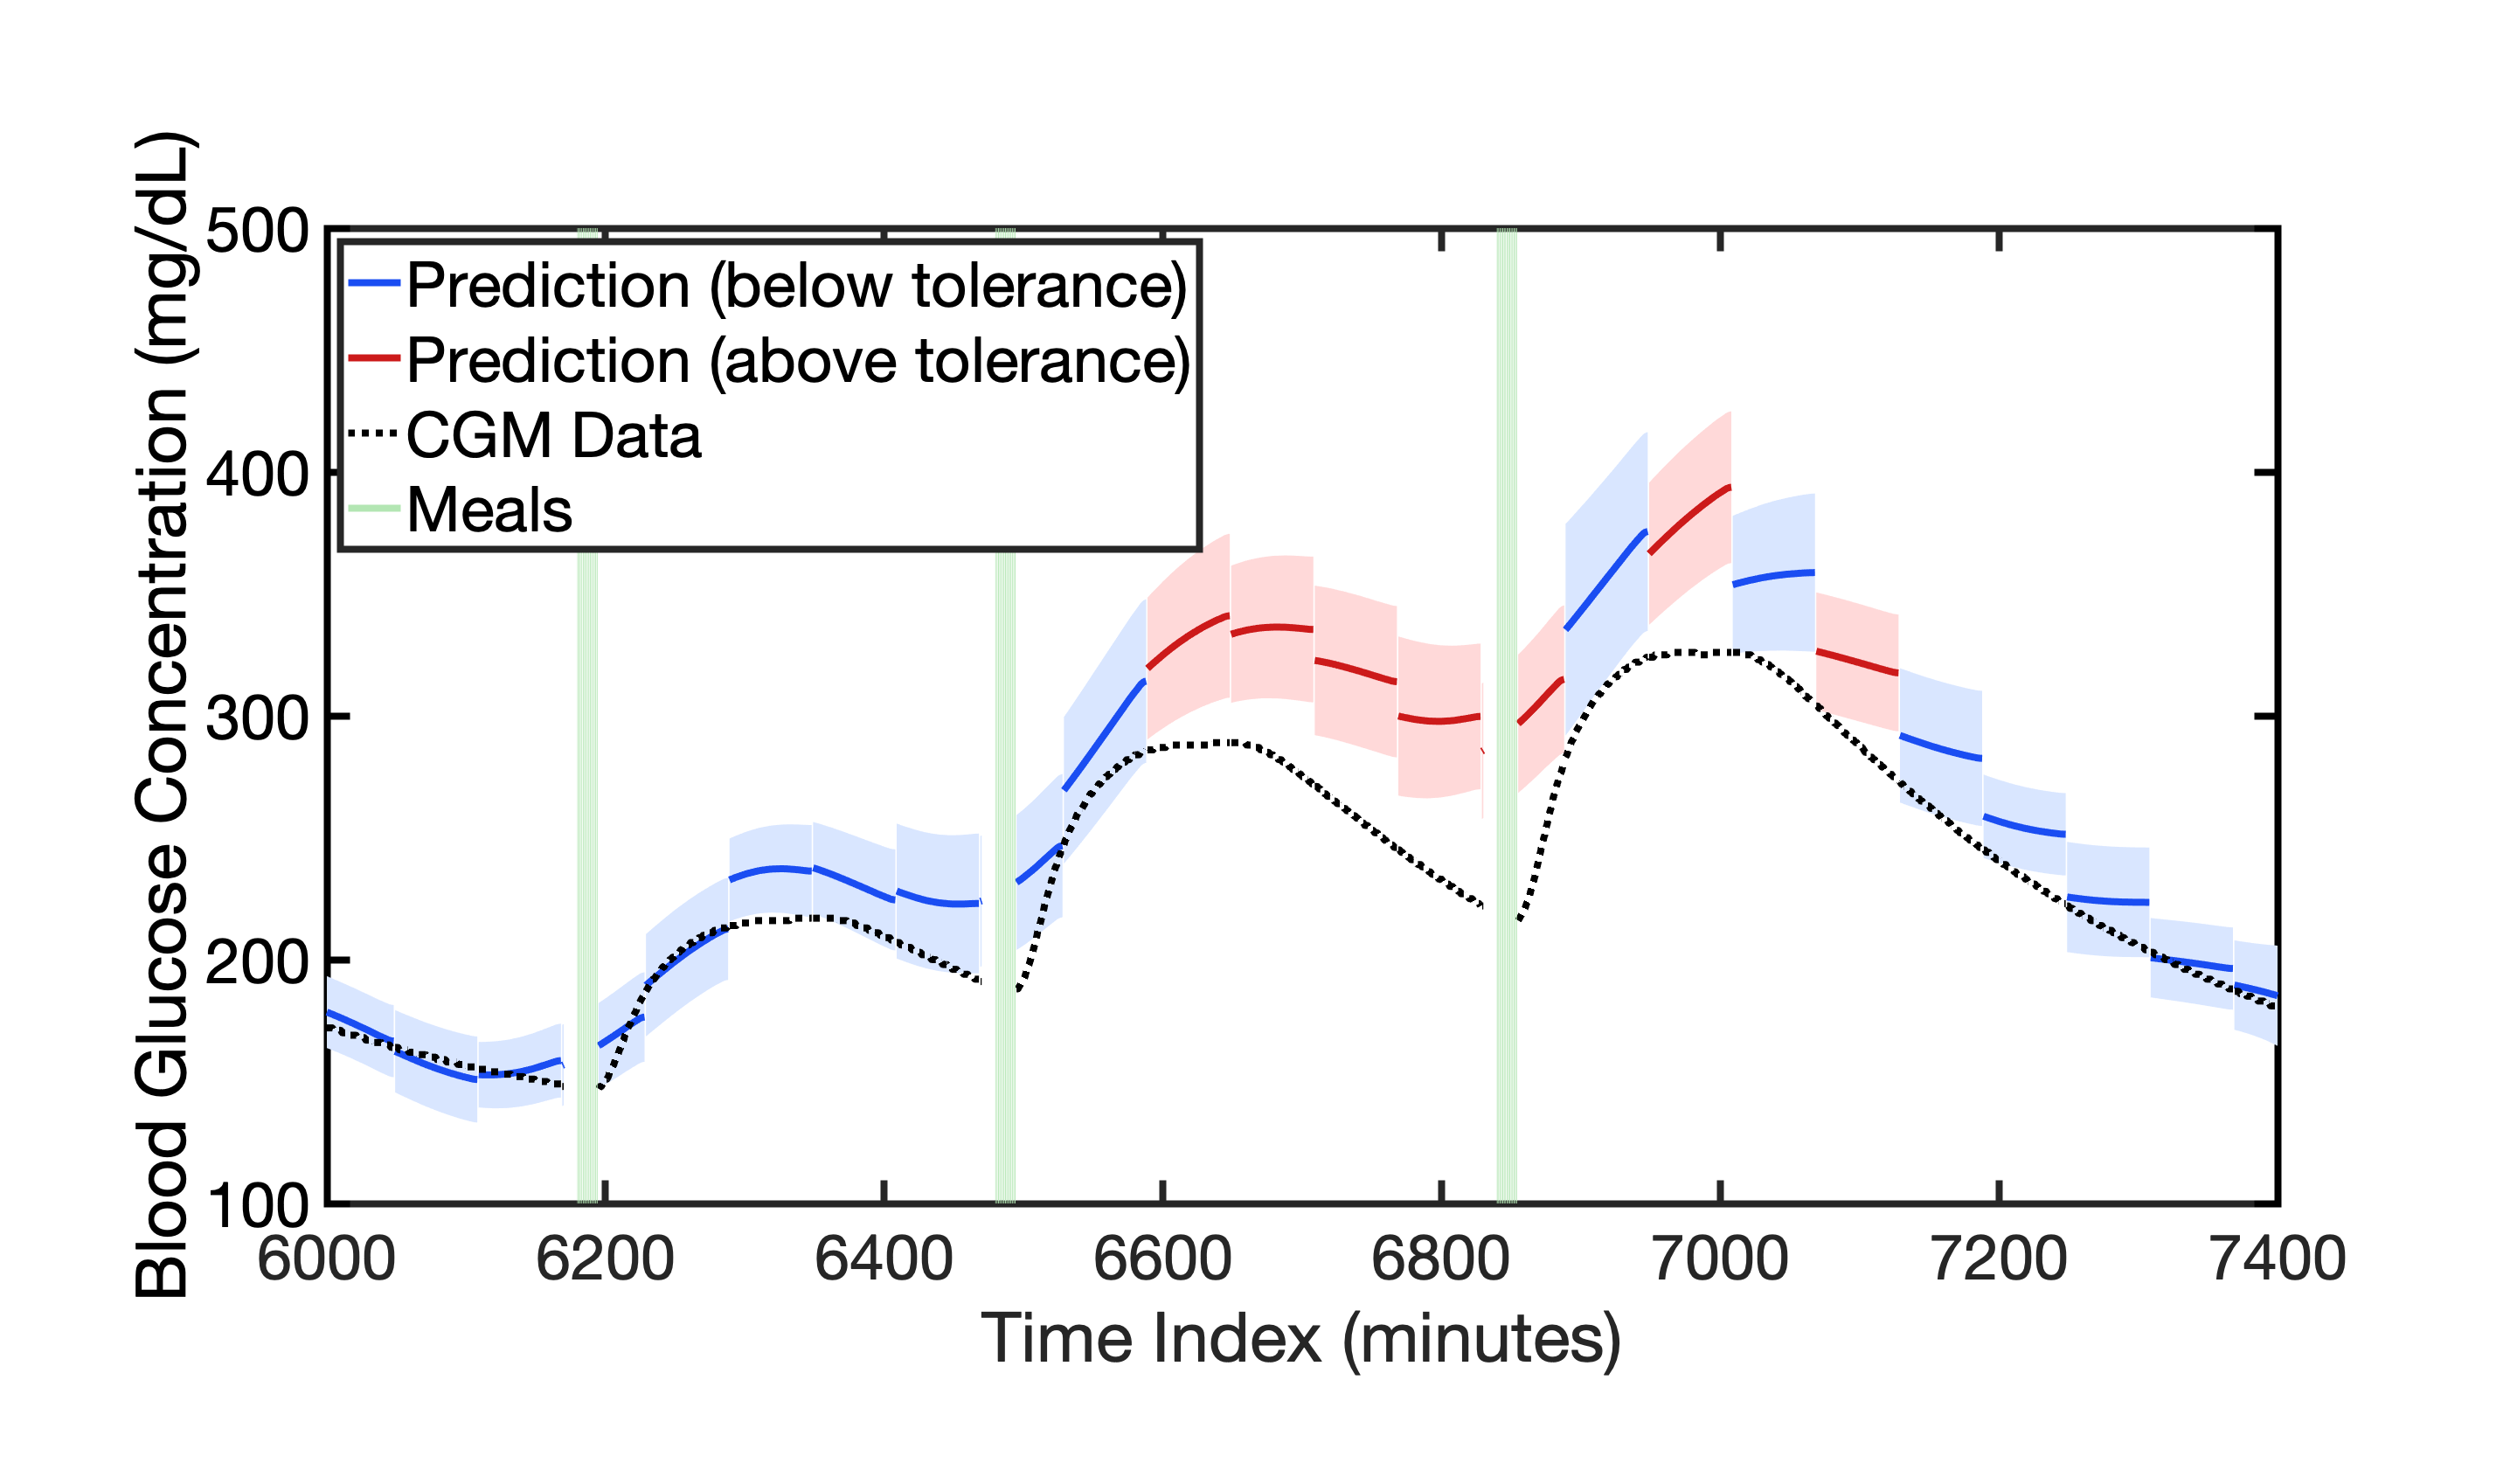
\includegraphics[width=0.45\linewidth]{Figures_manuscript/cat3_p4_c3.png}
  \vspace{-0.1in}
  \\ (a) \hspace{2.5in} (b)
  \vspace{-0.1in}
\caption{Representative validation failures for Level~3 architectures on held-out patients. (a) Patient 1 from fold~3 using $Level_3Arch_{10}$ and (b) Patient 4 from fold~4 using $Level_3Arch_4$. Red segments indicate one-hour prediction windows that violate the acceptance criterion $NLPD \leq Tol$.}
\label{fig:pred_cat3}
\end{figure}


%----Parks error map
\paragraph{Clinical risk mapping}
To complement NLPD-based validation, we evaluate representative rejected and accepted architectures using the Parkes error grid \cite{parkes2000new, pfutzner2013technical}, a clinically established mapping for assessing the impact of glucose prediction errors on treatment decisions. The grid partitions errors into risk zones including no clinical impact (Zone A), minimal clinical consequence (Zone B), incorrect action affecting
clinical outcome (Zone C), significant medical risk (Zone D), and 
to dangerous treatment decisions (Zone E).
%
Figure~\ref{fig:parkes} compares a rejected Level~1 architecture with the selected Level~2 model. To account for uncertainty, we overlay uncertainty bands from both CGM measurements noise and TCN predictions. While the mean predictions of the Level~1 model appear reasonable, its uncertainty spreads into higher-risk regions (primarily Zone B), indicating potential for clinically suboptimal decisions. In contrast, the selected Level~2 architecture concentrates predictions and associated uncertainty within Zone A, indicating clinically safe behavior. This comparison confirms that EVIDENT’s validation under uncertainty step also aligned with clinically meaningful risk criteria.

\begin{figure}[!ht]
\centering
\begin{minipage}[t]{0.5\textwidth}
  \centering
  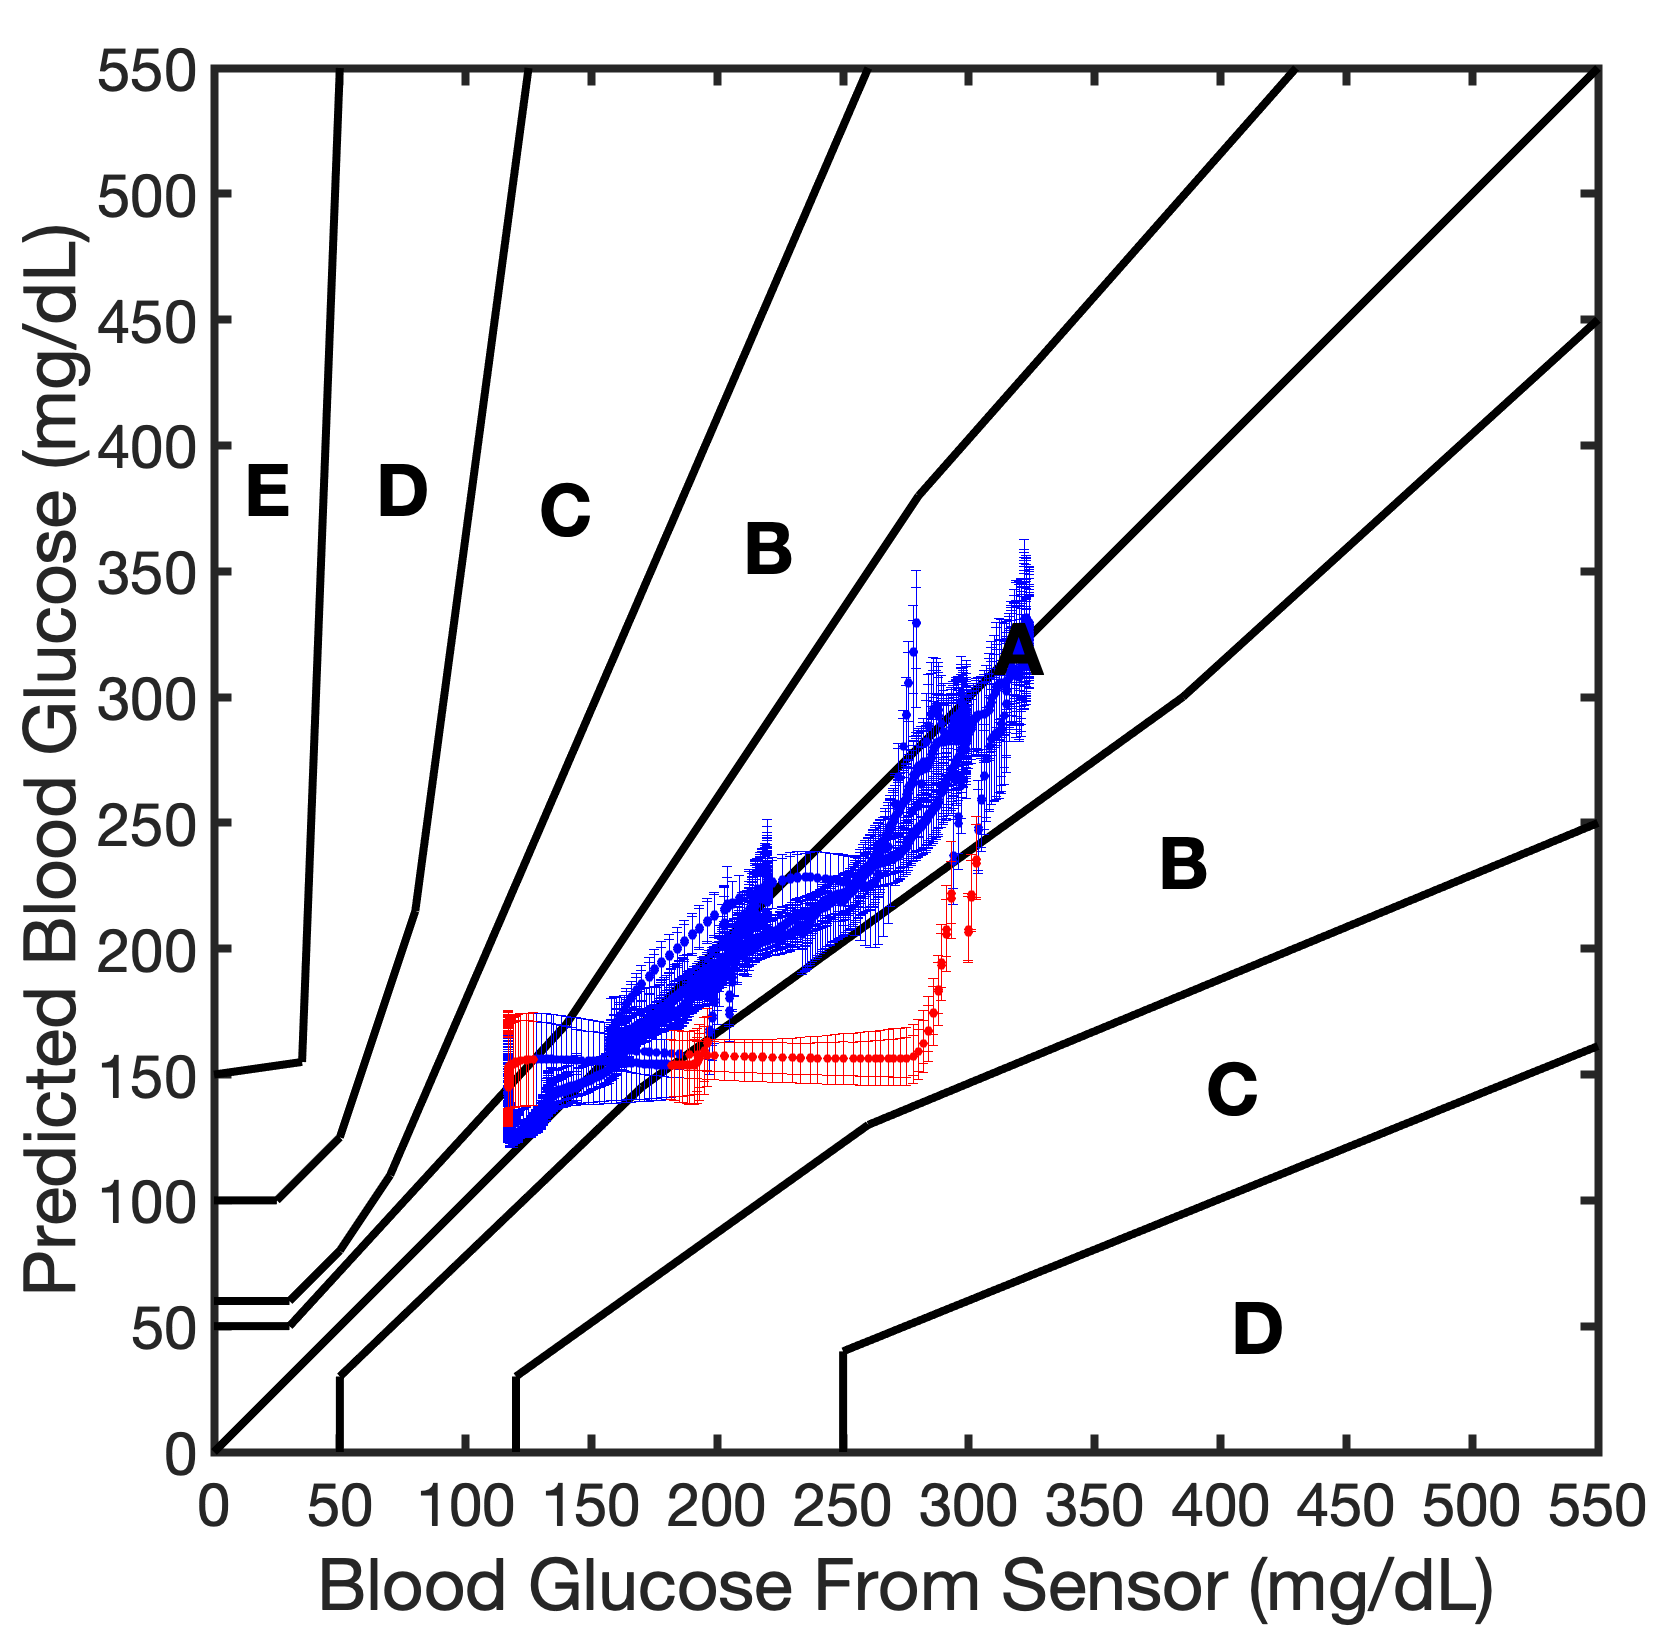
\includegraphics[width=0.75\linewidth]{Figures_manuscript/error_grid_bad.png}
  \caption*{(a)}
\end{minipage}\hfill
\begin{minipage}[t]{0.5\textwidth}
  \centering
 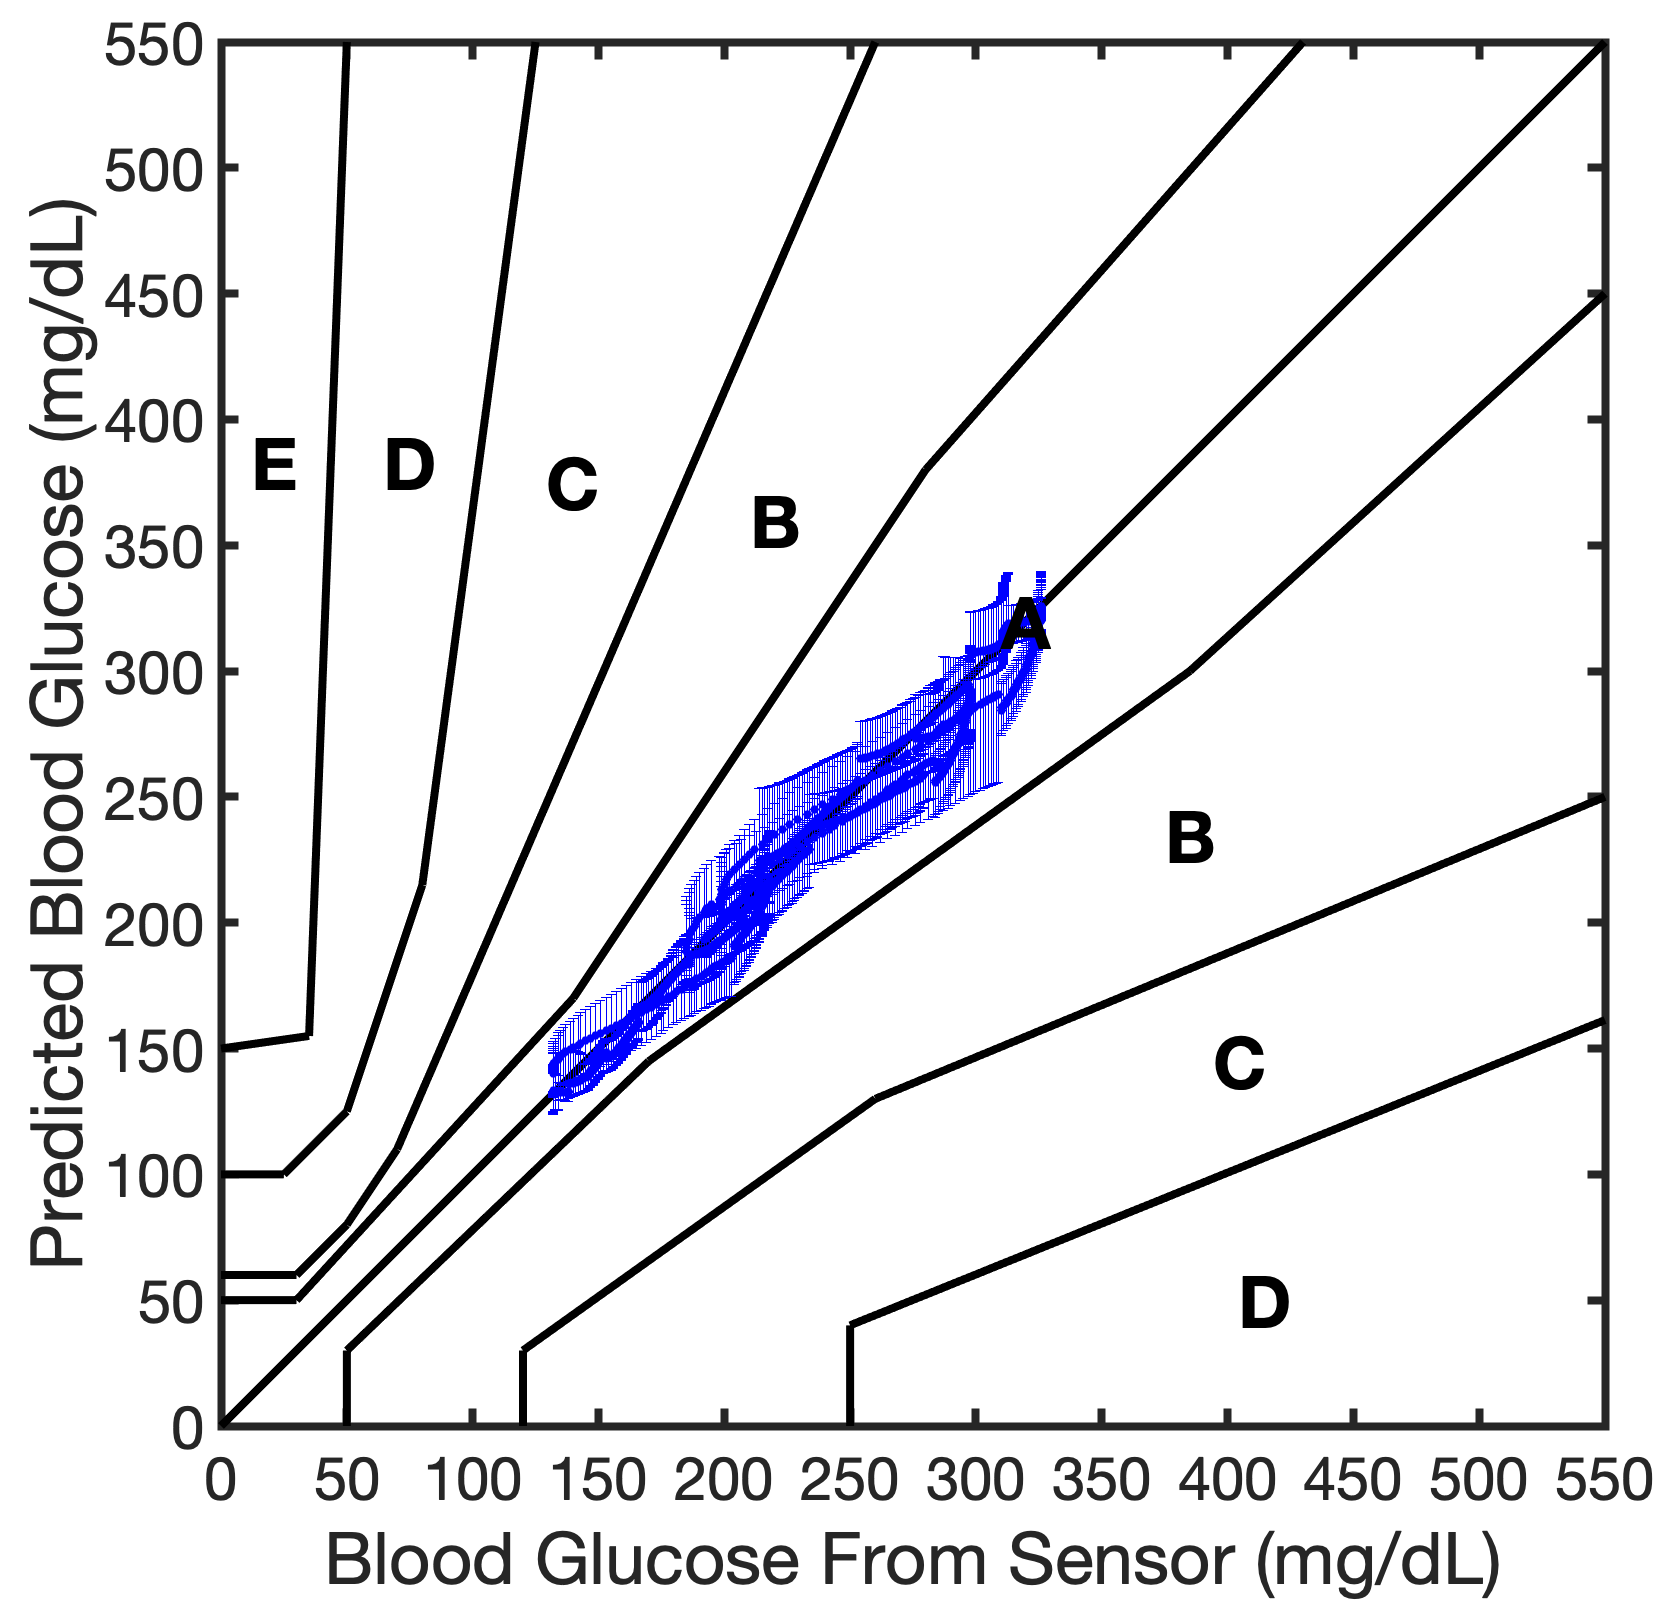
\includegraphics[width=0.75\linewidth]{Figures_manuscript/error_grid_good.png}
  \caption*{(b)}
\end{minipage}
\caption{Clinical risk assessment using the Parkes error grid for representative rejected and accepted architectures by EVIDENT. (a) Rejected Level~1 architecture ($Level_1Arch_1$) shows uncertainty extending into higher-risk Zone B. 
(b) Selected Level~2 architecture ($Level_2Arch_4$) concentrates predictions within Zone A, corresponding to clinically safe decisions.}
\label{fig:parkes}
\end{figure}


%++++++++++++++++++++++++++++++++++++++++++++++++++++++++++++++++++++++++
\subsection{Random-search baseline}
\label{sec:baseline}

To provide a baseline for architecture discovery, we compared EVIDENT against random search with similar budget. Random search is a standard baseline for hyperparameter and architecture selection because it provides a non-adaptive sampling strategy and has been shown to be competitive with grid search under fixed computational budgets \cite{bergstra2012random}. In contrast to EVIDENT, 
which progressively narrows the candidate space through evidence-guided ranking and validation across ordered capacity levels, random search samples architectures uniformly from the feasible pool and selects models solely based on held-out performance.

%

The baseline study uses the same pool of 61 feasible TCN architectures and the same population-based to subject-specific prediction protocol employed in the EVIDENT experiments. To approximately match the computational budget required by EVIDENT up to acceptance, random search samples 19 architectures uniformly without replacement from the feasible candidate pool, corresponding to the total number of architectures evaluated in Levels~1 and~2. The sampled architectures are listed in ~\ref{app:architecture_pool}
where to distinguish incomplete architecture coverage from the selection rule itself, we considered a random-search subset that included the EVIDENT-selected architecture, denoted here as $RandArch_6=Level_2Arch_4$.
Each sampled architecture is first trained on the population training subjects within the corresponding fold. For each held-out subject, the resulting population posterior is then used as the prior for subject-specific adaptation using three days of patient data. Architecture selection is subsequently performed on day 4 using rolling one-hour prediction windows, where the selected architecture minimizes the NLPD across the held-out subjects. Consistent with the EVIDENT protocol, day 5 is excluded from model selection and reserved exclusively for final comparison with EVIDENT results.

%
\begin{figure}
\centering
\begin{minipage}[t]{0.5\textwidth}
  \centering
  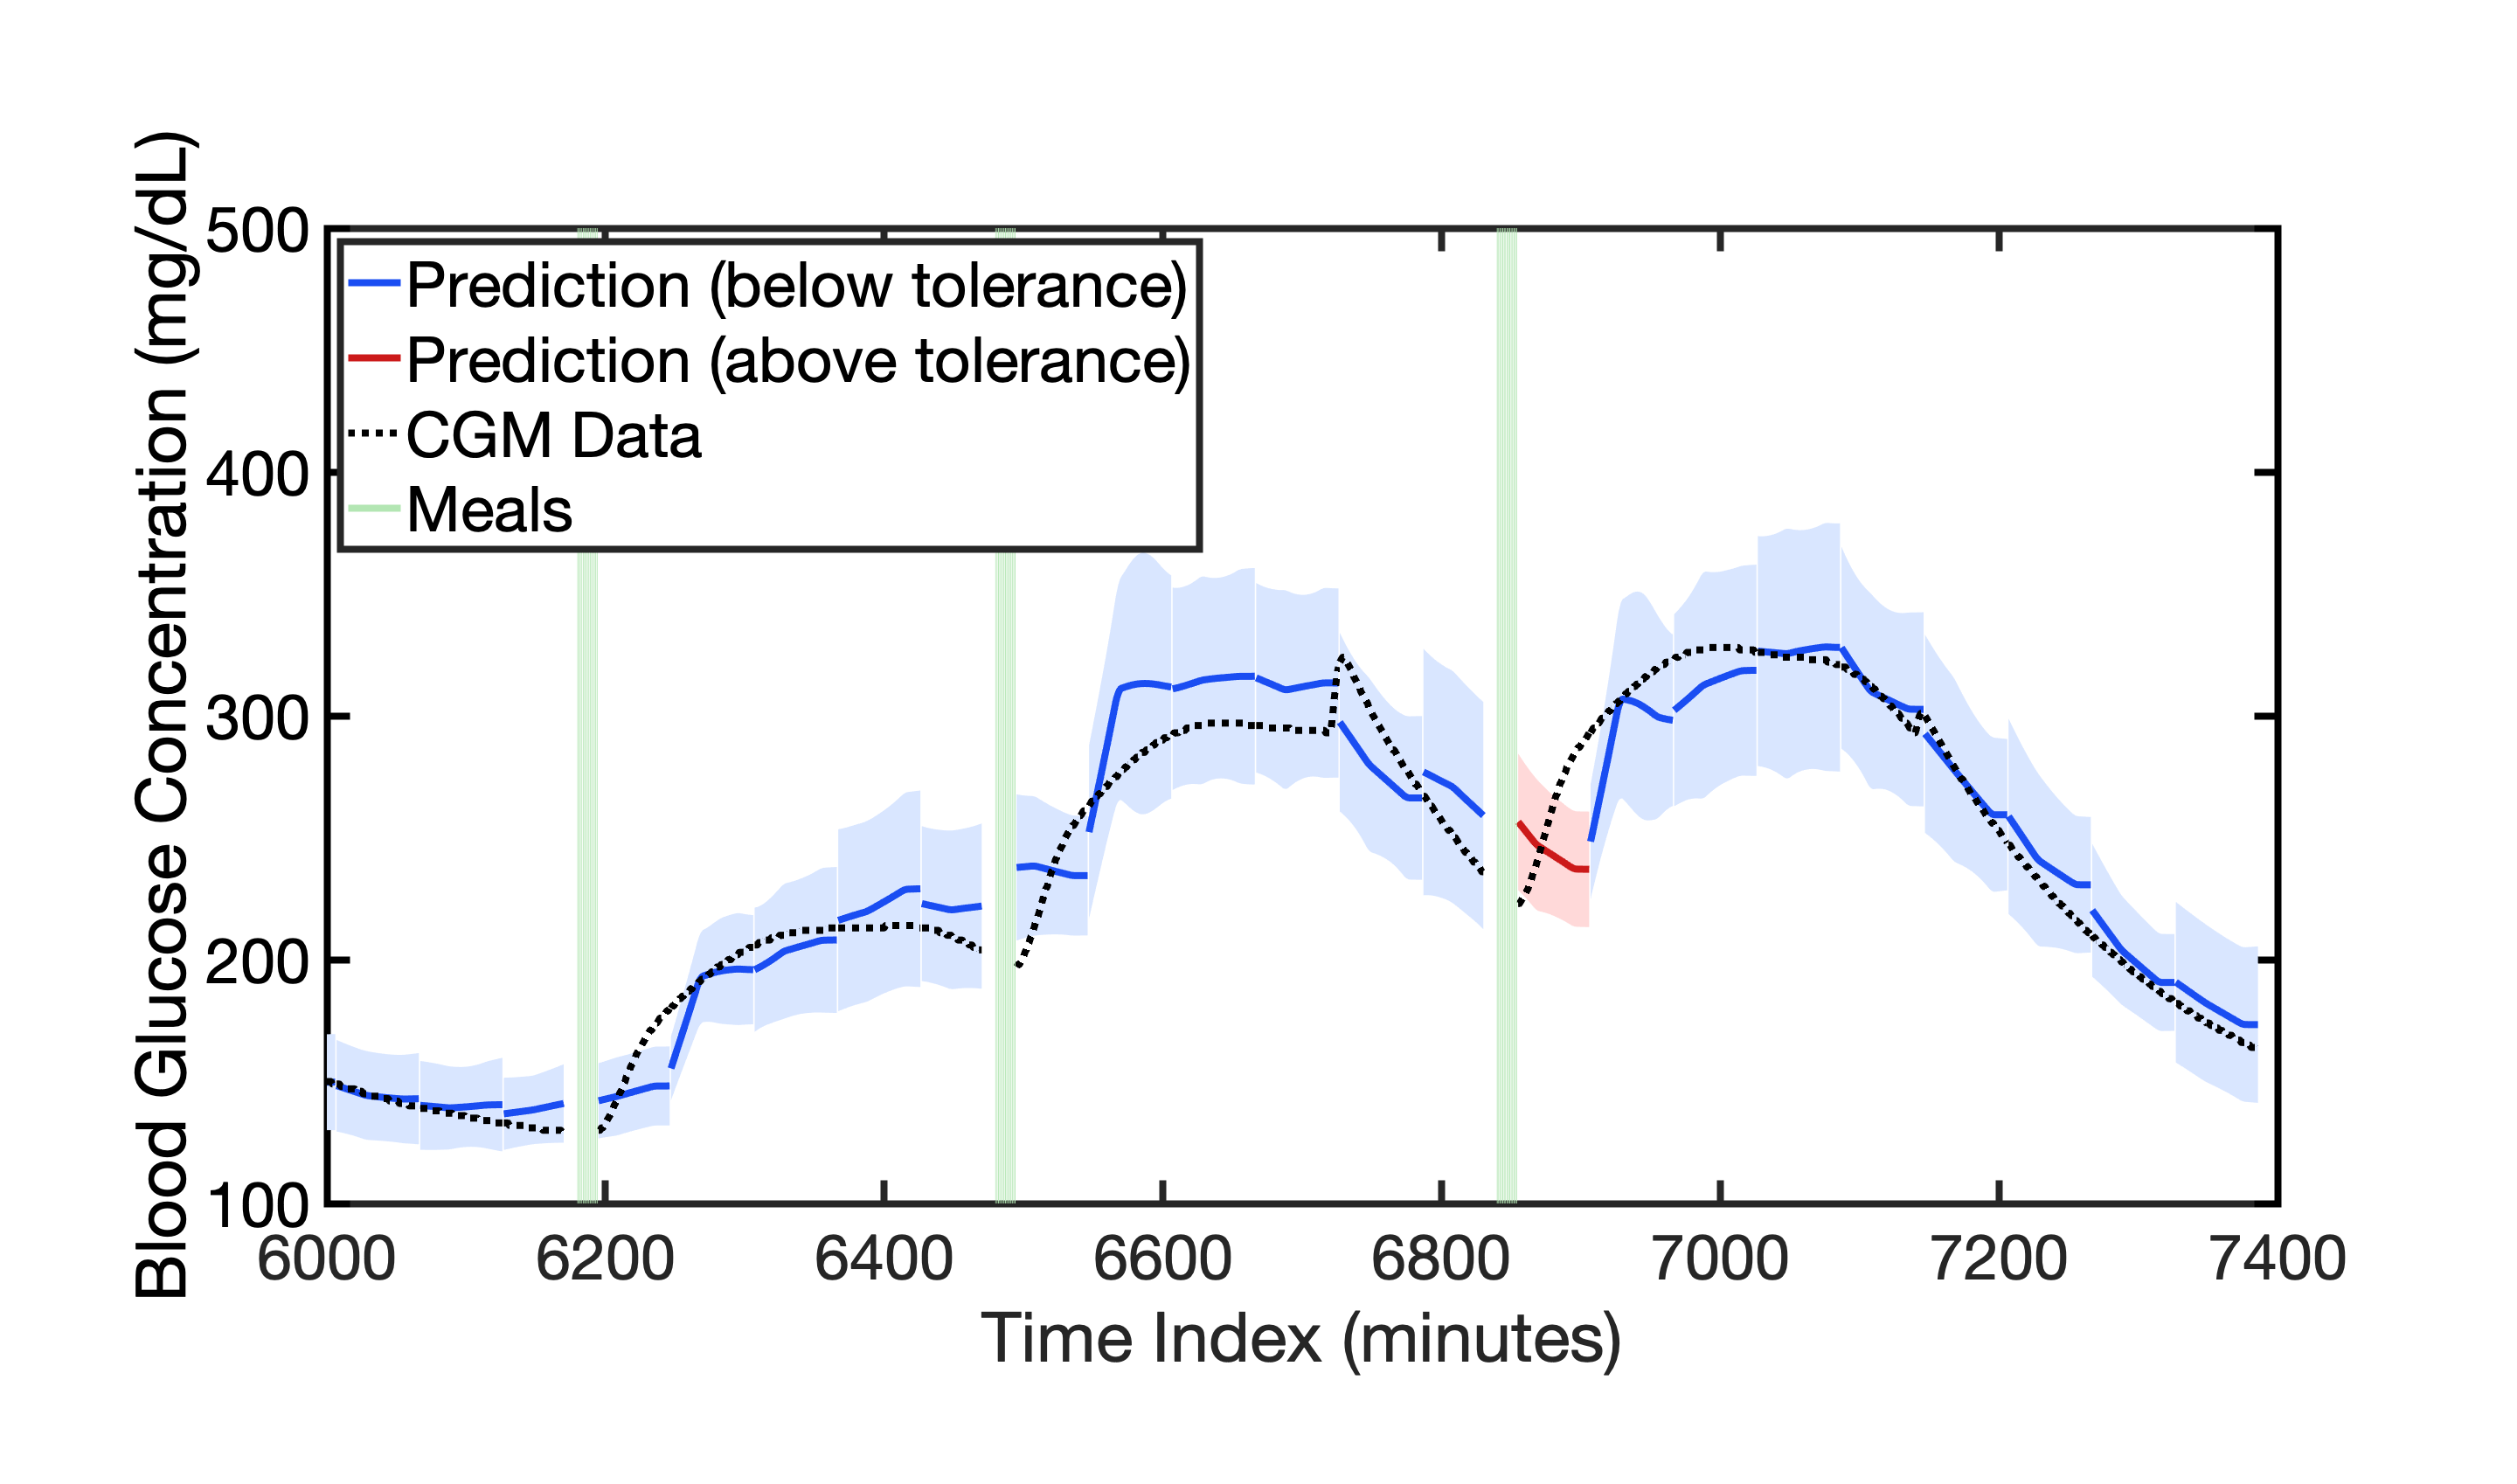
\includegraphics[width=\linewidth]{Figures_manuscript/cat3_d5f7_random_p3.png}
  \caption*{(a)}
\end{minipage}\hfill
\begin{minipage}[t]{0.5\textwidth}
  \centering
  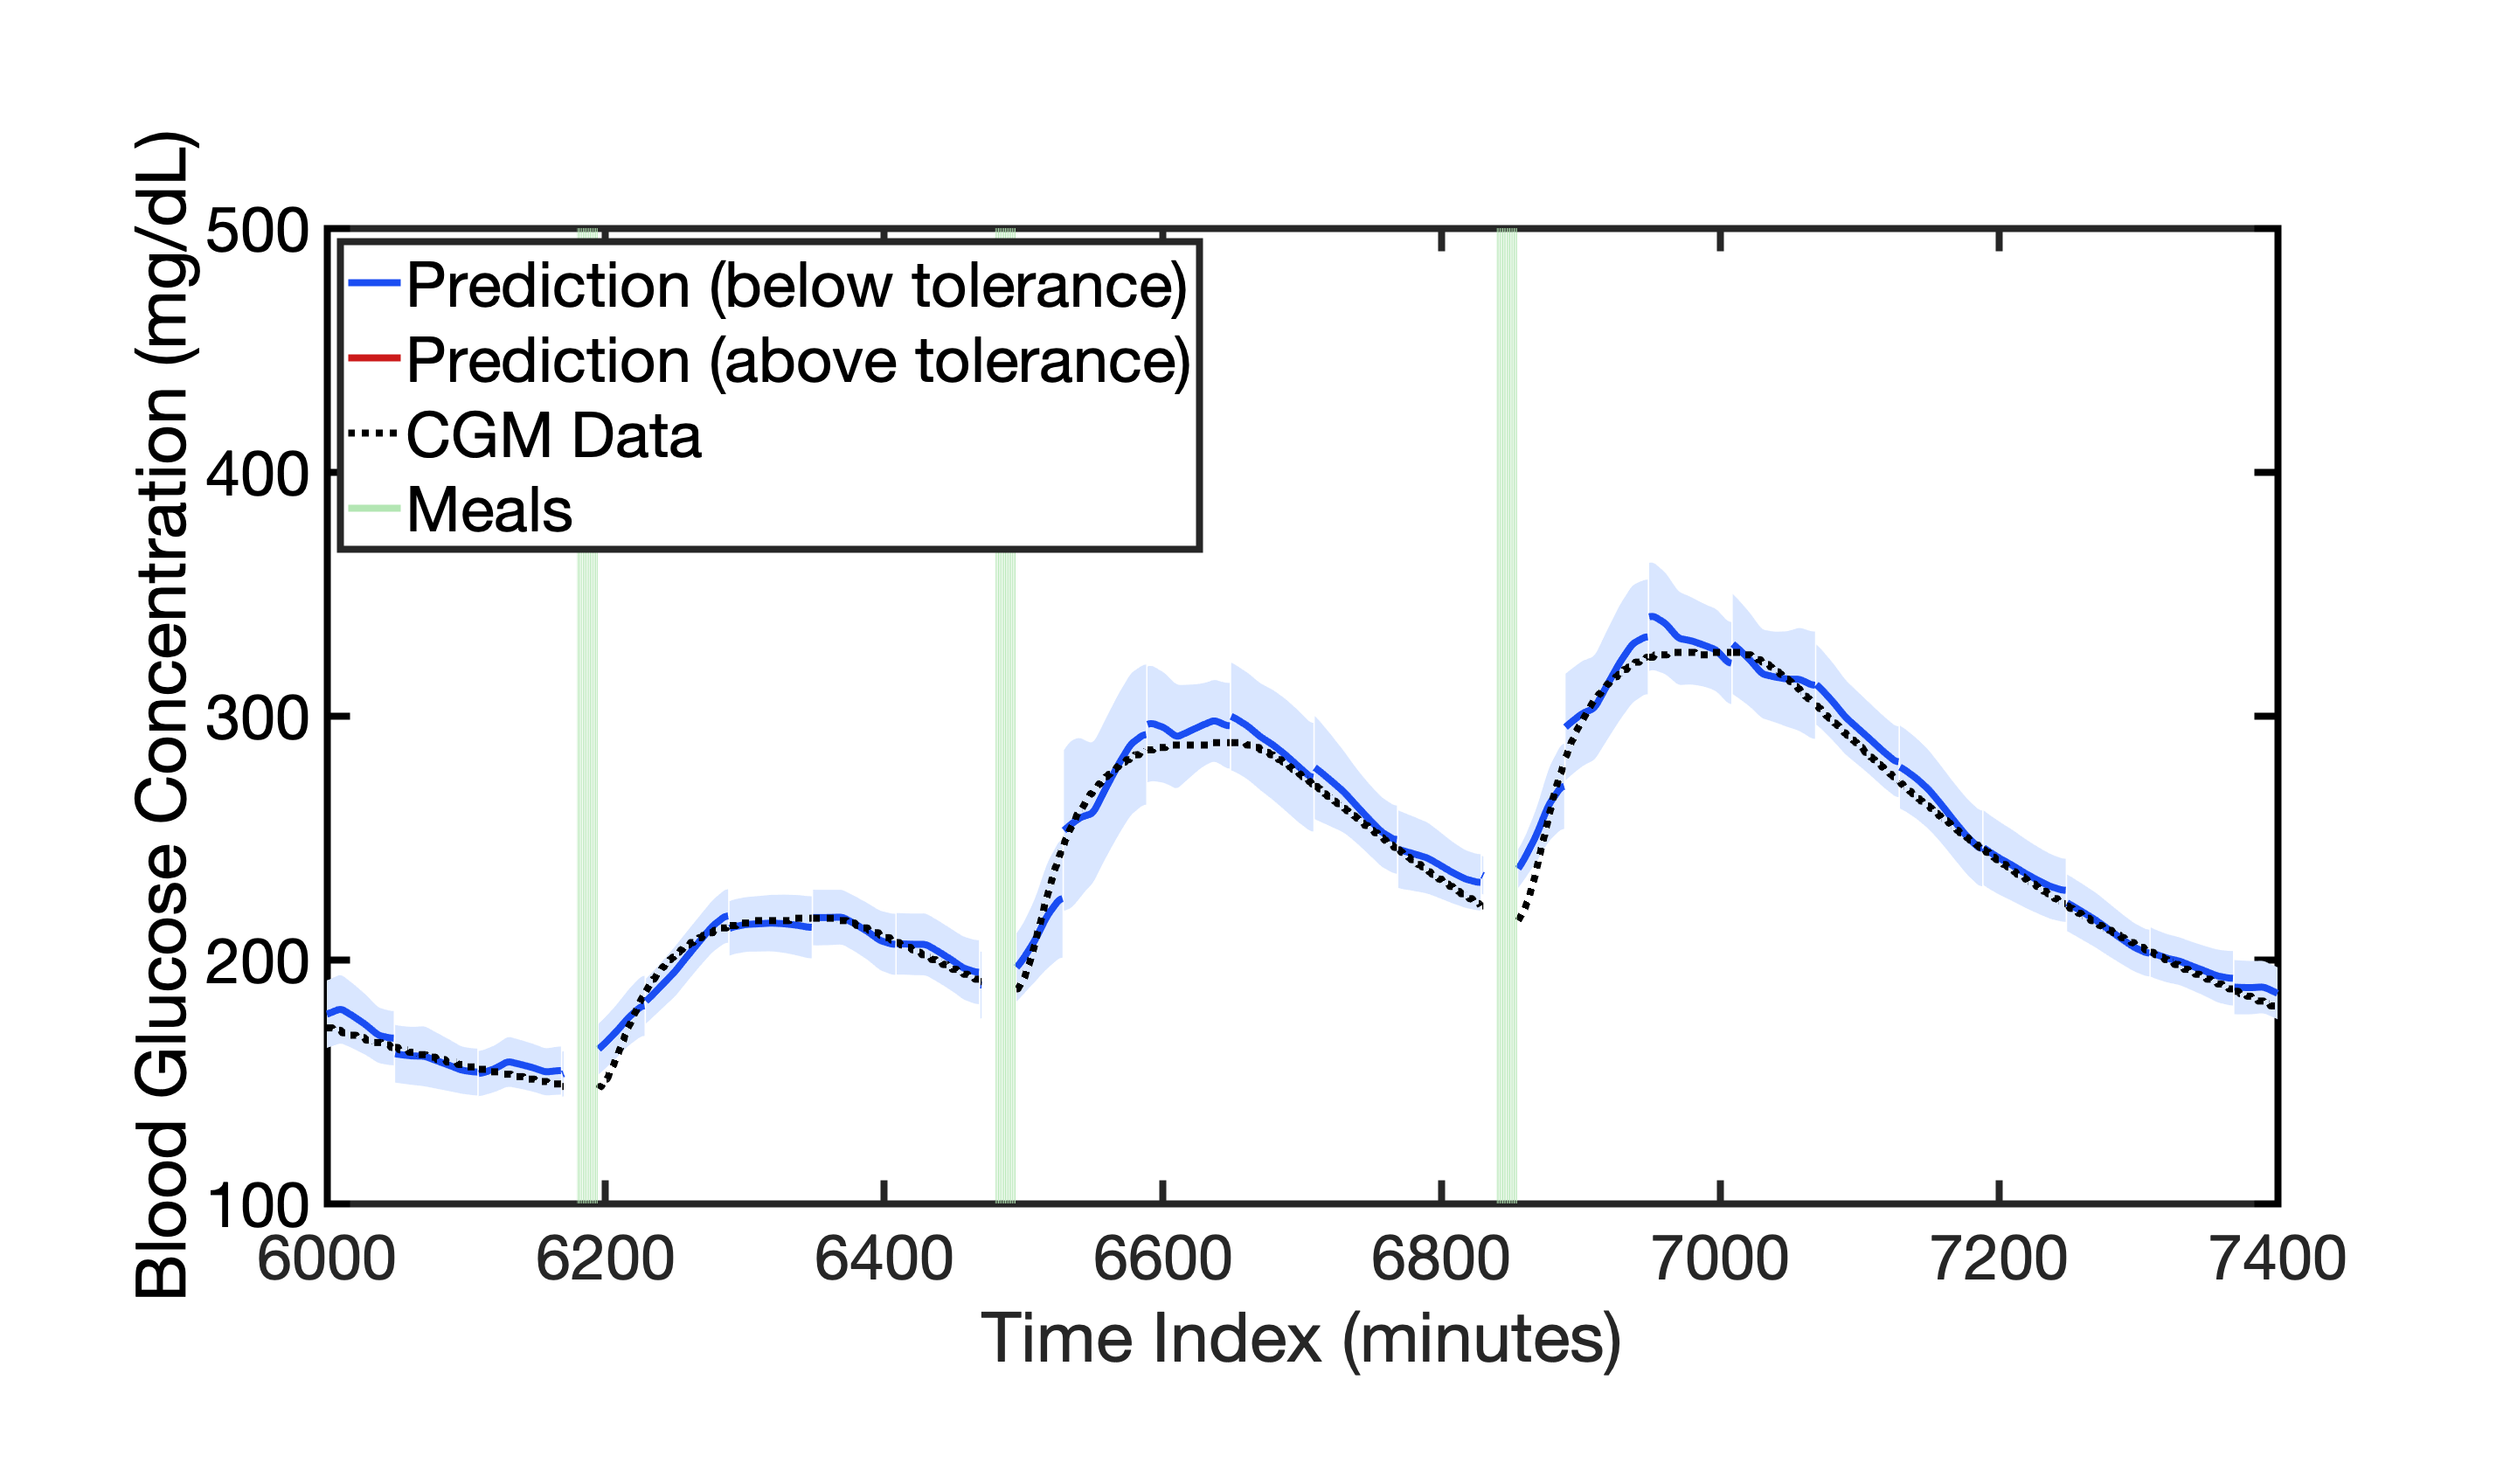
\includegraphics[width=\linewidth]{Figures_manuscript/cat3_d5f7_random_p4.png}
  \caption*{(b)}
\end{minipage}
\begin{minipage}[t]{0.5\textwidth}
  \centering
  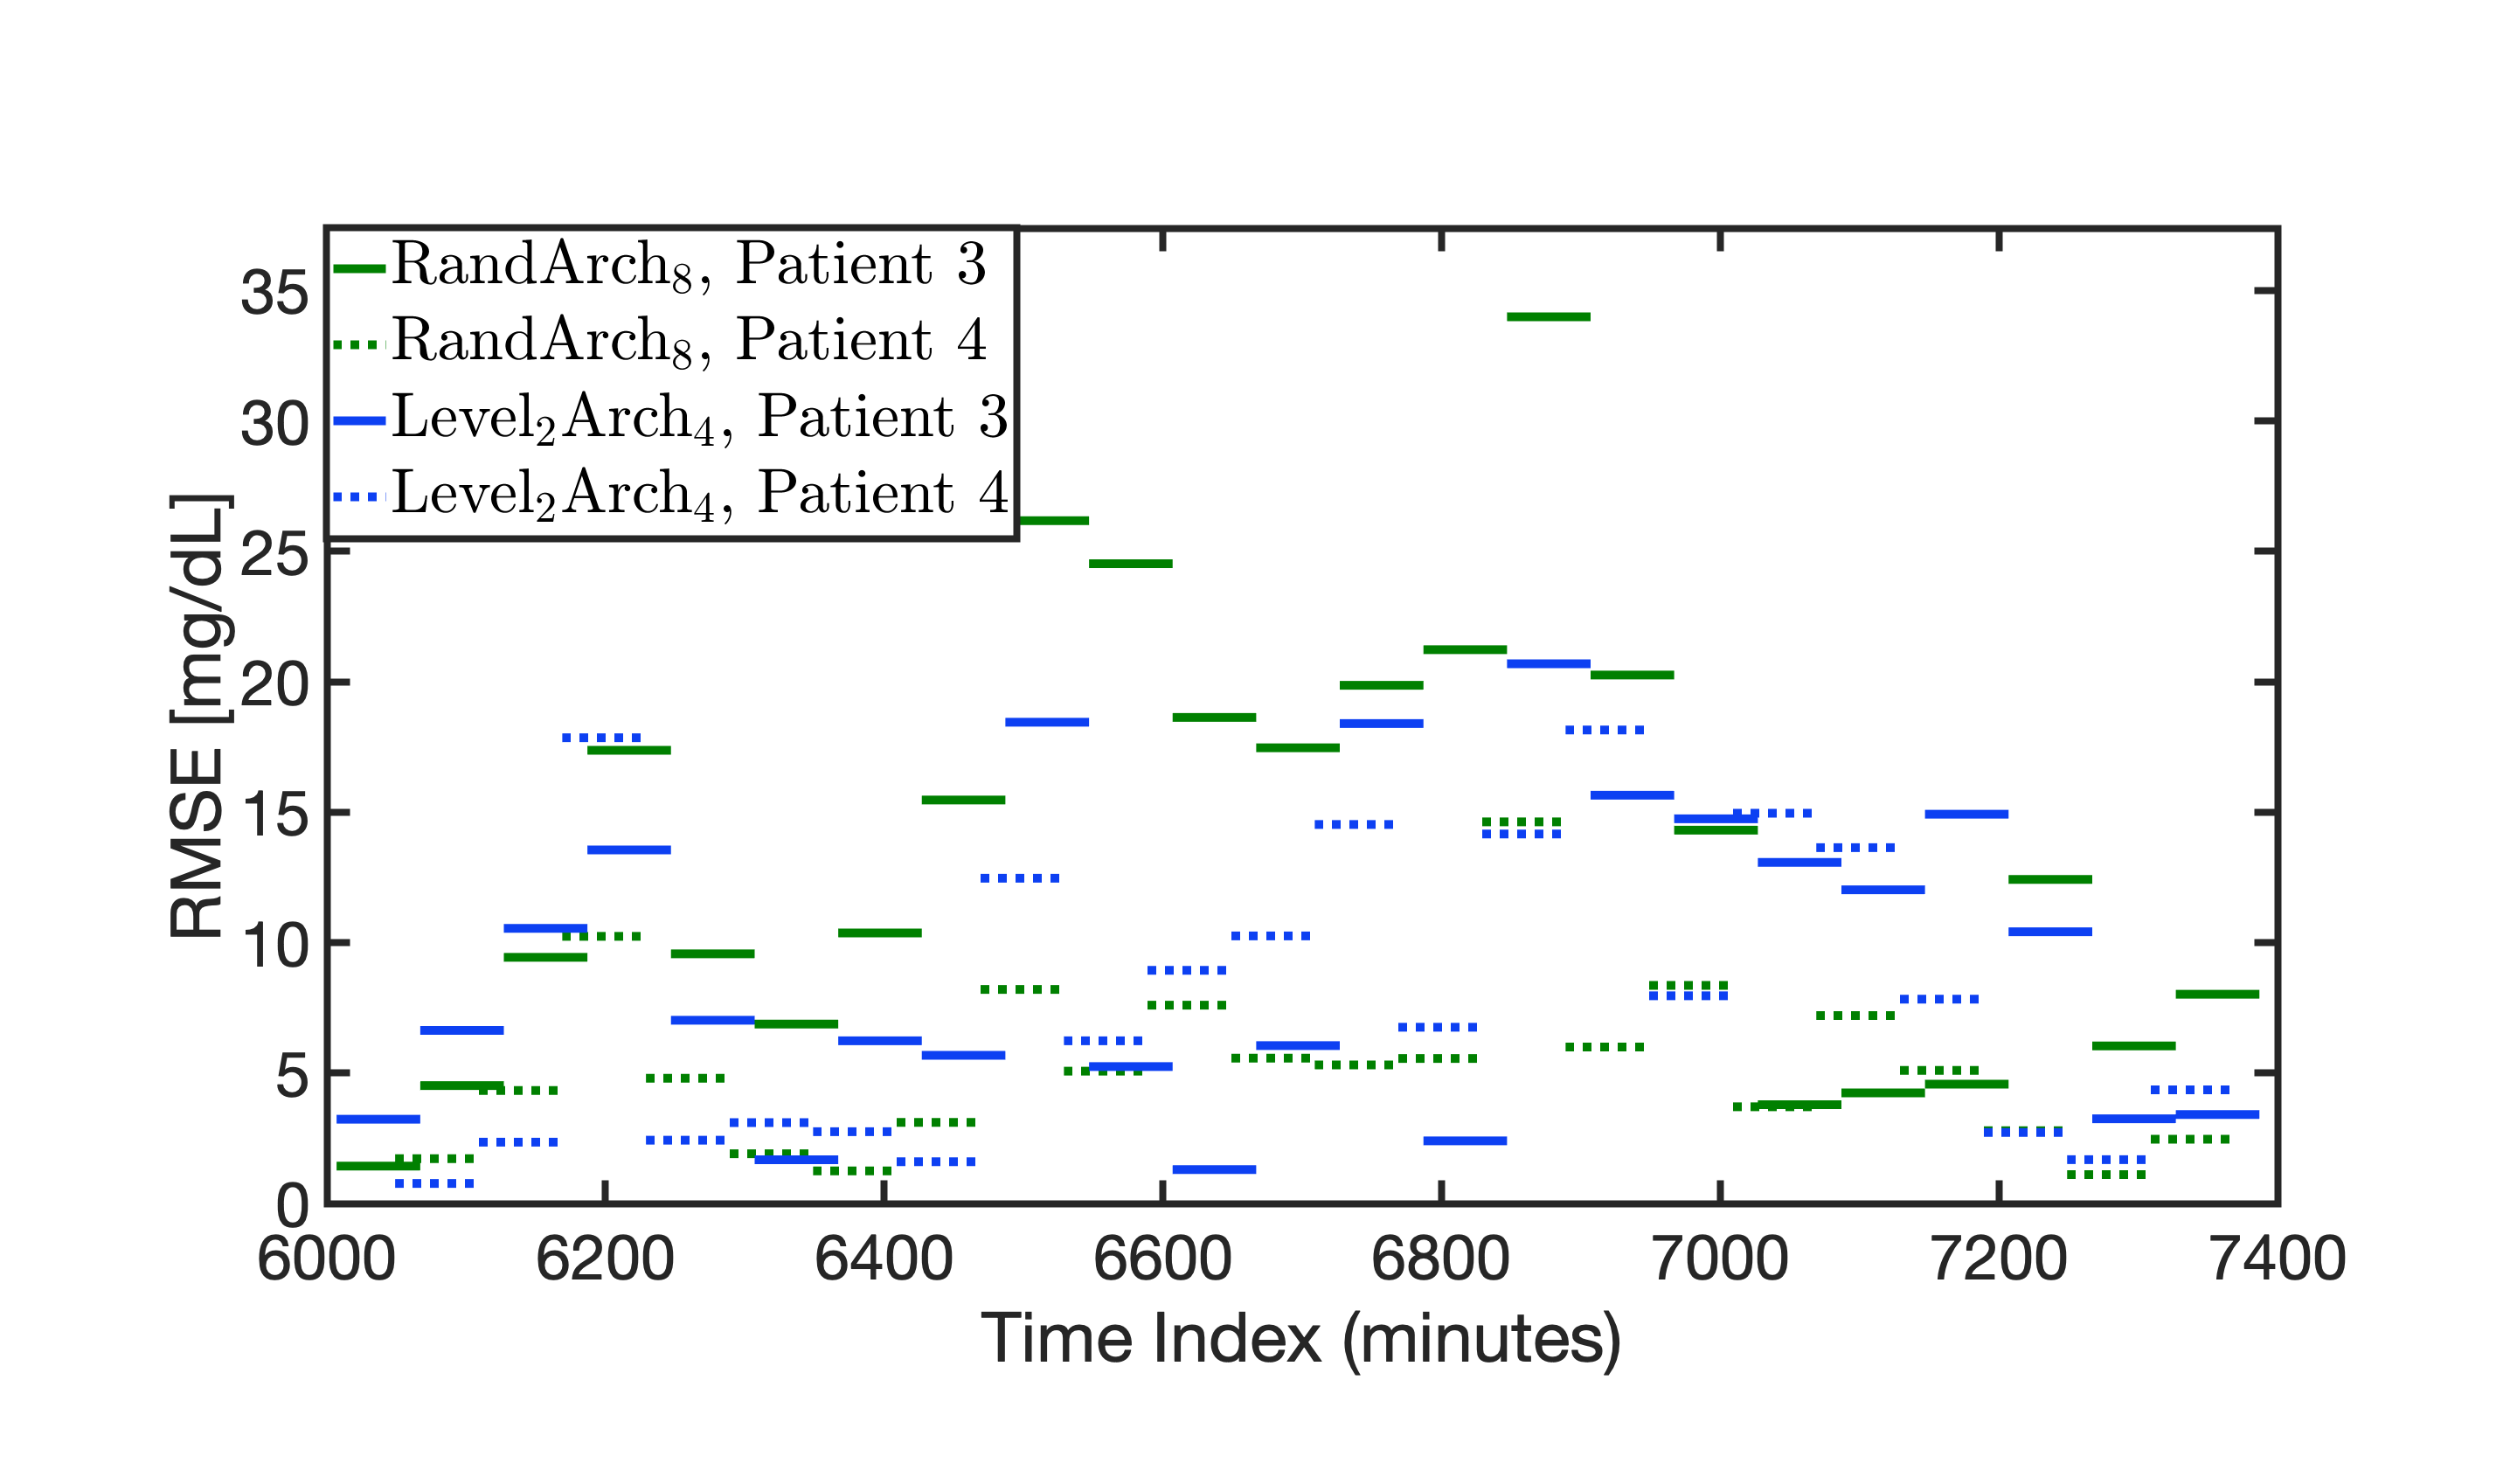
\includegraphics[width=\linewidth]{Figures_manuscript/RMSE_rand.png}
  \caption*{(c)}
\end{minipage}\hfill
\begin{minipage}[t]{0.5\textwidth}
  \centering
  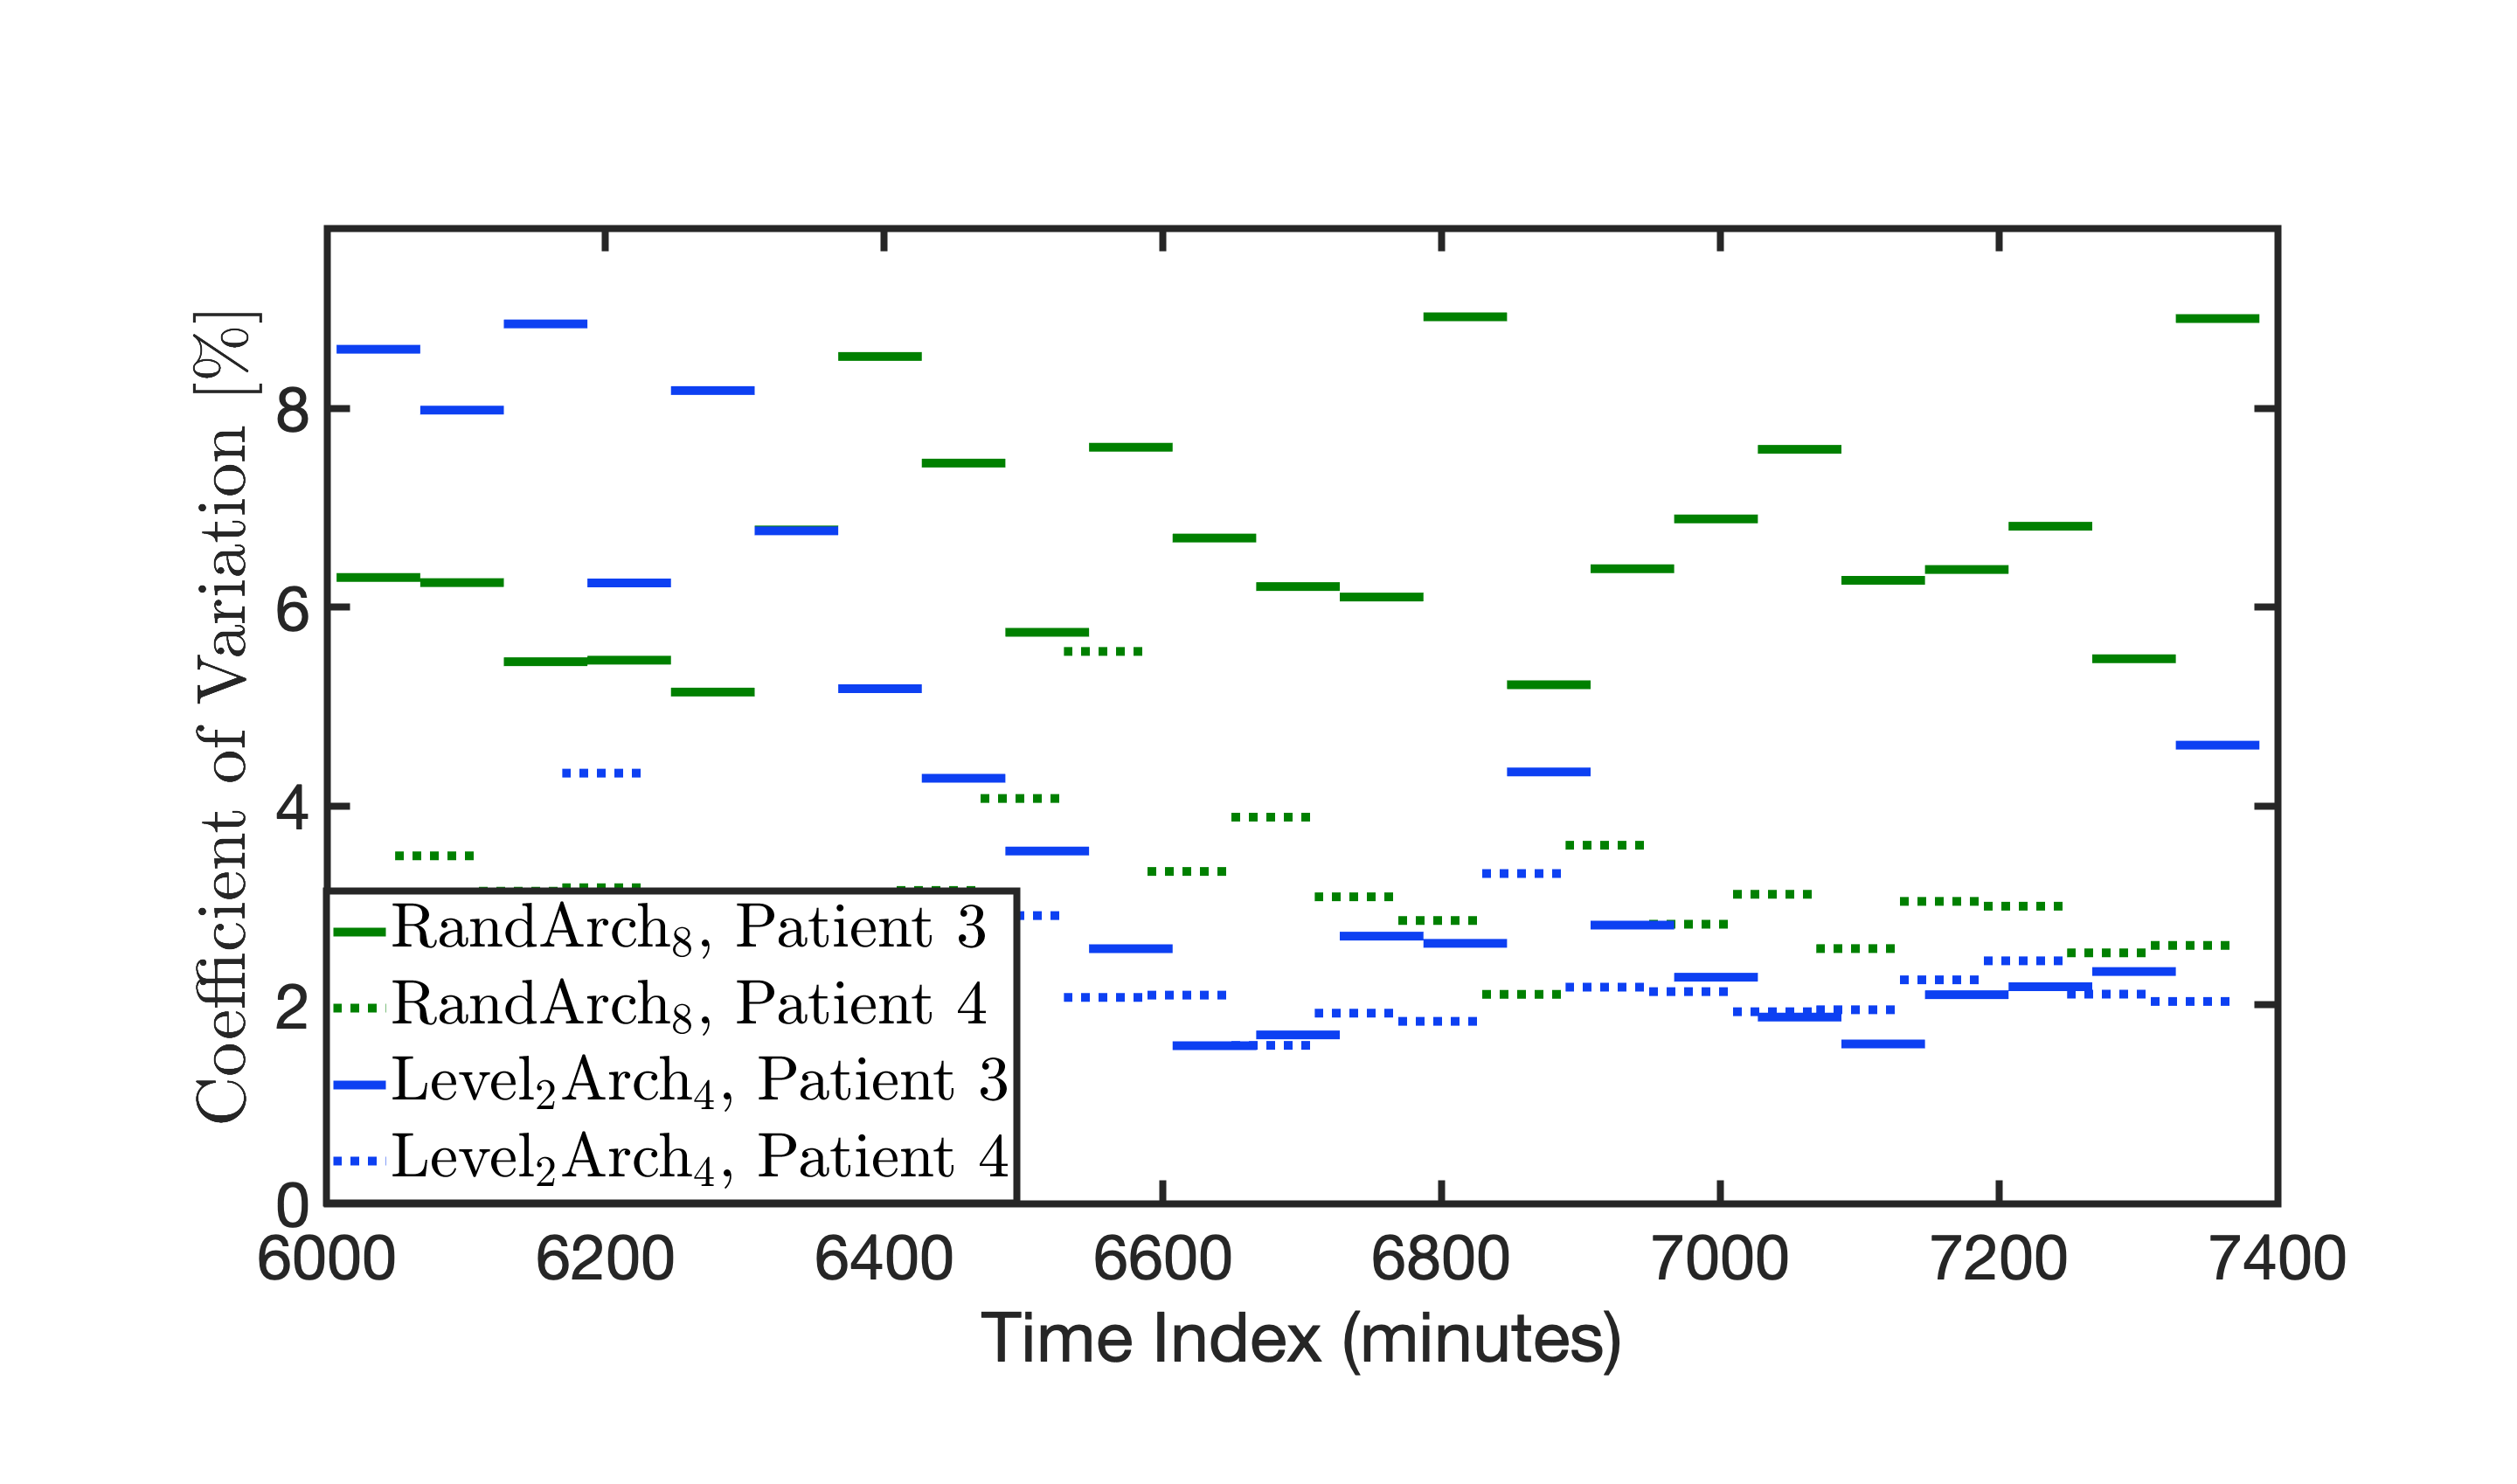
\includegraphics[width=\linewidth]{Figures_manuscript/CV_rand.png}
  \caption*{(d)}
\end{minipage}
\begin{minipage}[t]{0.48\textwidth}
  \centering
  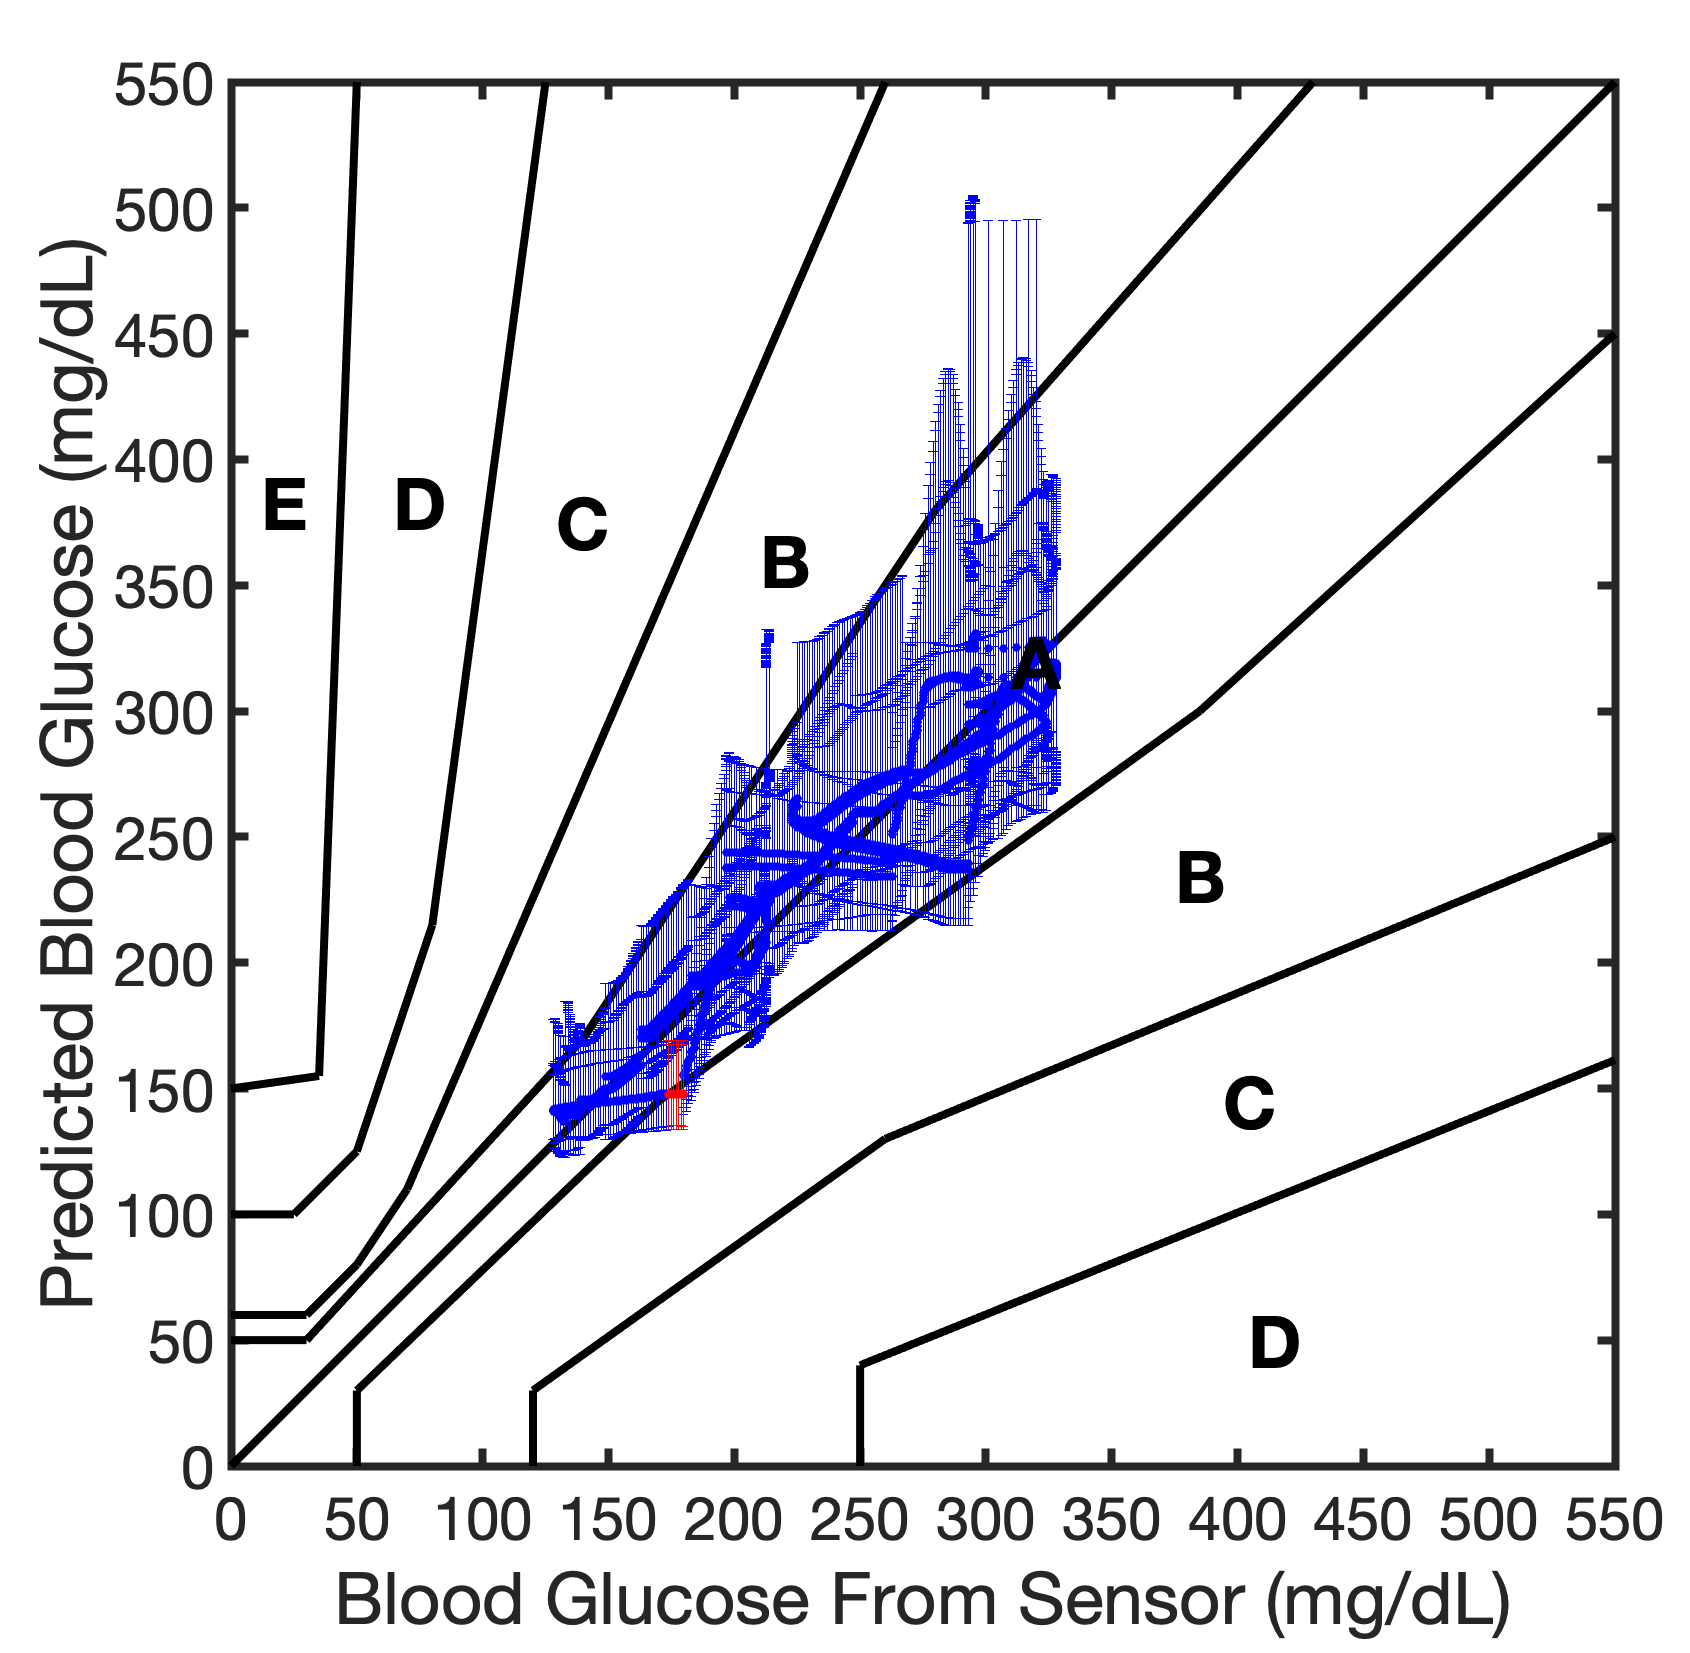
\includegraphics[width=0.8\linewidth]{Figures_manuscript/parkes_p3_rand.png}
  \caption*{(e)}
\end{minipage}\hfill
\begin{minipage}[t]{0.48\textwidth}
  \centering
  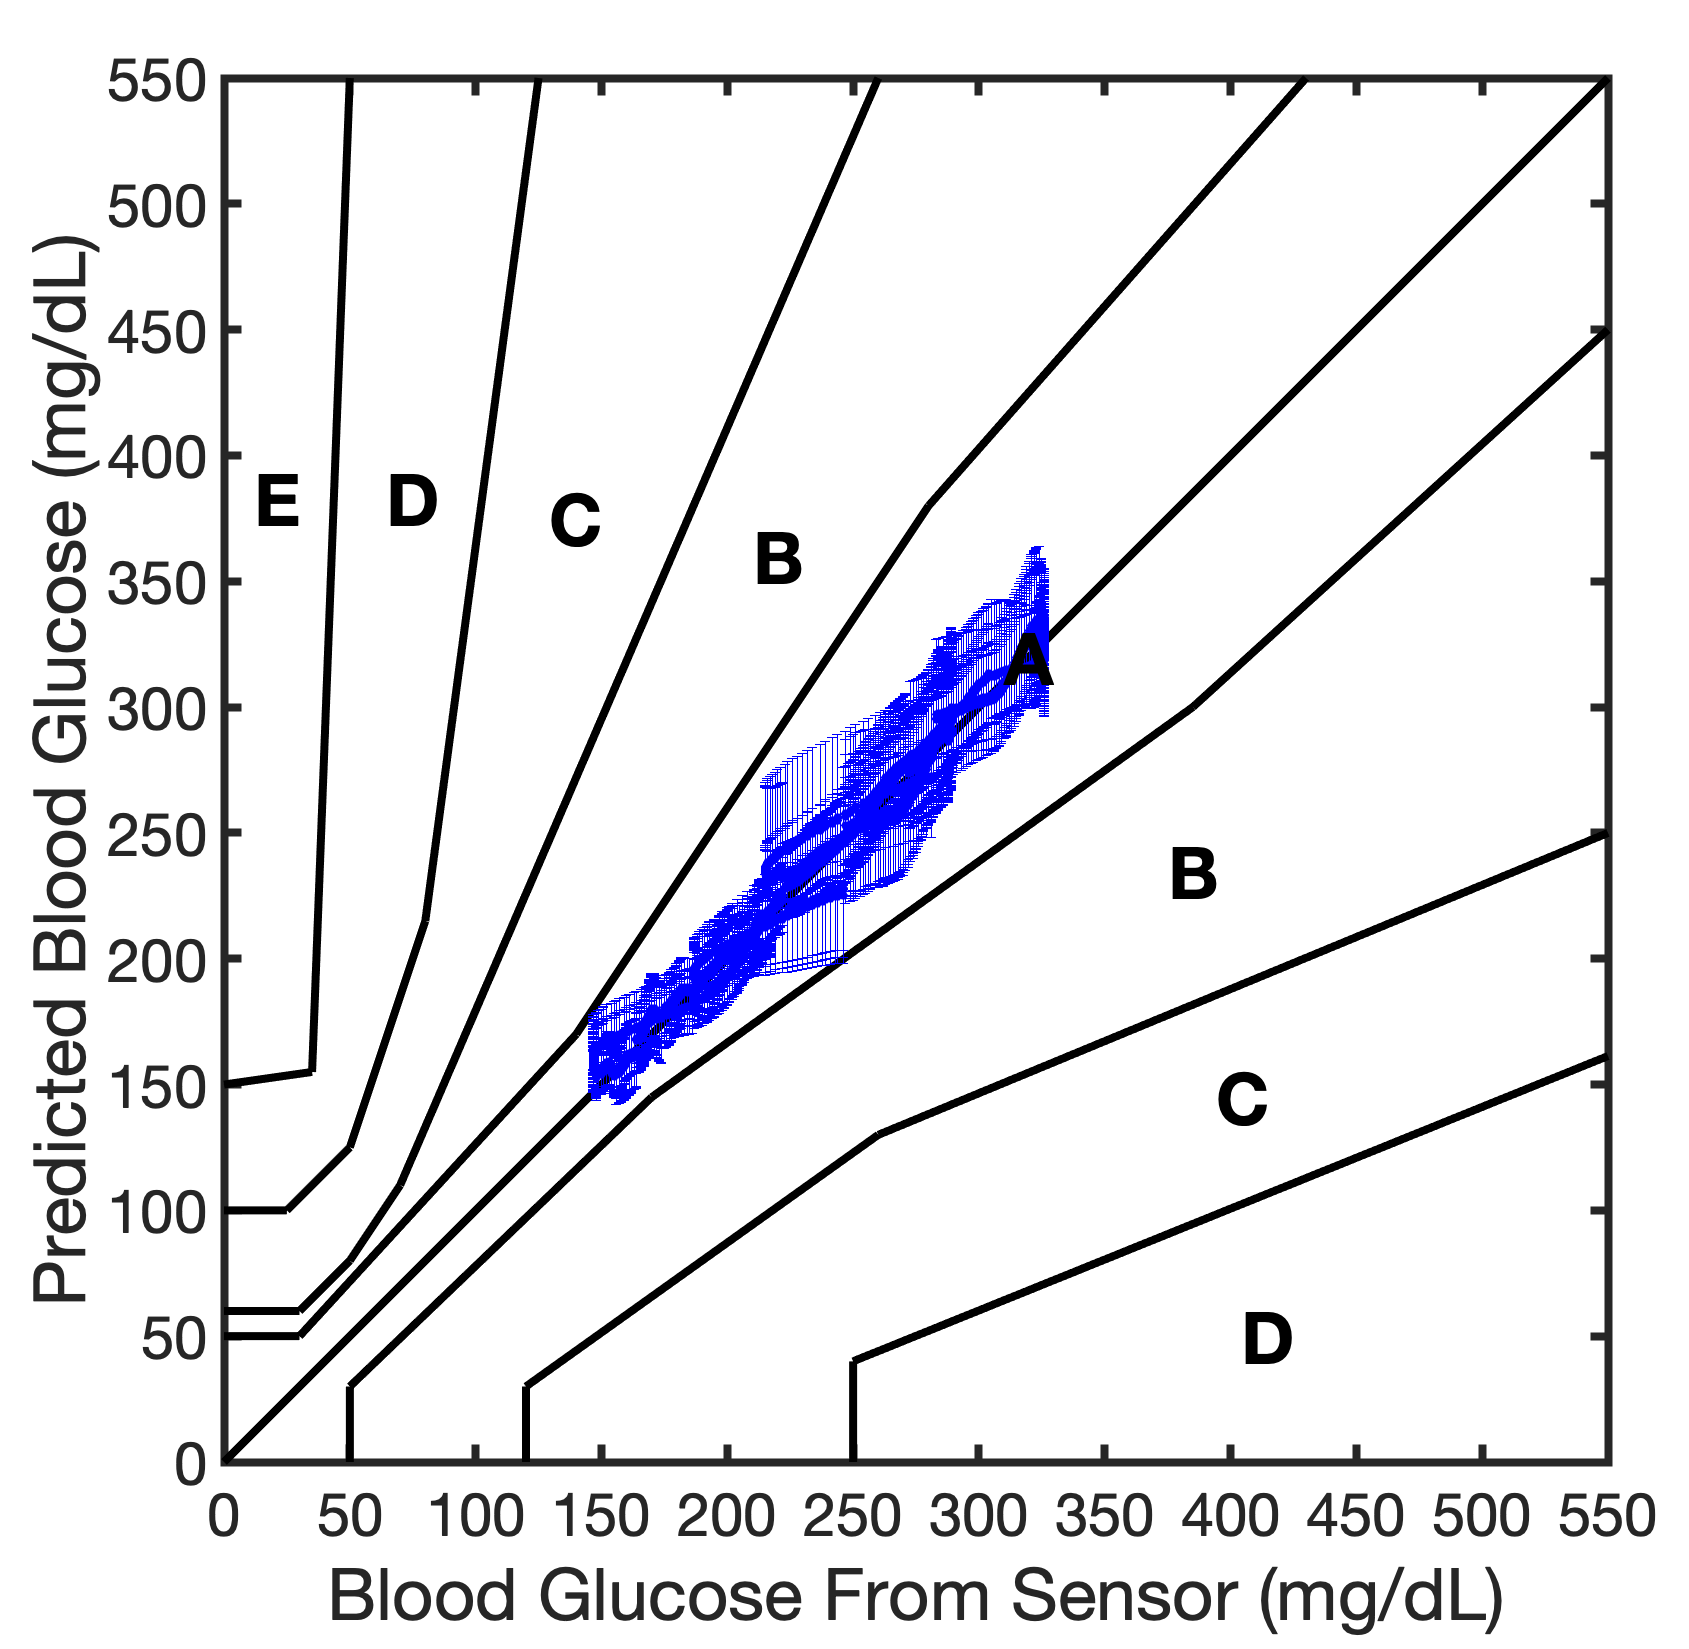
\includegraphics[width=0.8\linewidth]{Figures_manuscript/parkes_rand_p4.png}
  \caption*{(f)}
\end{minipage}
\caption{
Performance comparison between the random-search-selected architecture $RandArch_8$ and the EVIDENT-selected architecture $Level_2Arch_4$ for the held-out patients in Fold 4. (a,b) show the 1-hour rolling glucose predictions of $RandArch_8$ for patients 3 and 4, respectively. 
(c) compares the corresponding rolling-window RMSE, while (d) compares the predictive coefficient of variation (\%CV). (e,f) show the Parkes error grid analysis for $RandArch_8$.}
\label{fig:random_search}
\end{figure}


The random-search criterion selects $RandArch_8$ due to lowest average day 4 validation NLPD for held-out patients even though $RandArch_6=Level_2Arch_4$ is in the 19 randomly selected architectures in Table \ref{tab:random}. $RandArch_8$ contains 133424 trainable parameters, with $N=4$, $f=7$, $b=5$, encoder channels $[8,16,32,64]$, and $\mathrm{RF}=1873$. In comparison, $Level_2Arch_4$ contains 43268 trainable parameters and has a similar receptive field, $\mathrm{RF}=1937$; its full architectural specification is reported in Table \ref{tab:level2}.
Thus, the two models have comparable temporal coverage, but $RandArch_8$ achieves it through a larger dilation base, wider filter size and more number of channels, leading to approximately three times more trainable parameters.


Figure~\ref{fig:random_search} compares the 1-hour rolling predictions of $RandArch_8$ for the held-out patients 3 and 4 in Fold 4.
%
For the diagnostic comparison in this figure, we also report the rolling-window root mean-squared error (RMSE) and coefficient of variation (CV), representing accuracy and reliability of TCN forecast respectively,
%
\begin{equation}
\mathrm{RMSE}
=
\left[
\frac{1}{H}
\left\|
G_{\mathrm{data}}^{(k+1:k+H)}
-
\overline{\mathcal{T}}_{w,\xi}\!\left(
G_{\mathrm{data}}^{(k-d_G:k)},
M_{\mathrm{data}}^{(k-d_M:k)},
I_{\mathrm{data}}^{(k-d_I:k)}
\right)
\right\|_2^2
\right]^{1/2},
\label{eq:rmse}
\end{equation}
%
and
%
\begin{equation}
\mathrm{CV}
=
\frac{100}{H}
\sum_{h=1}^{H}
\frac{
\sqrt{
\mathrm{Var}\!\left[
\mathcal{T}_{w,\xi}^{(k+h)}\!\left(
G_{\mathrm{data}}^{(k-d_G:k)},
M_{\mathrm{data}}^{(k-d_M:k)},
I_{\mathrm{data}}^{(k-d_I:k)}
\right)
\right]
}
}{
\left|
\overline{\mathcal{T}}_{w,\xi}^{(k+h)}\!\left(
G_{\mathrm{data}}^{(k-d_G:k)},
M_{\mathrm{data}}^{(k-d_M:k)},
I_{\mathrm{data}}^{(k-d_I:k)}
\right)
\right|
}.
\label{eq:cv}
\end{equation}
%
Here, $h$ indexes the forecast step within the $H$-step prediction horizon, $\overline{\mathcal{T}}_{w,\xi}$ is the posterior predictive mean, and $\mathrm{Var}[\mathcal{T}_{w,\xi}^{(k+\ell)}]$ is the posterior predictive variance at forecast step $k+\ell$.
%
The rolling-window RMSE and CV show that this additional capacity does not translate into more reliable validation performance. 
For patient 3, $RandArch_8$ exhibits larger RMSE over several one-hour windows and higher predictive CV, resulting in failure under the NLPD validation criterion. For patient 4, $RandArch_8$ attains lower RMSE in some windows, but this subject-specific improvement is not consistent across the held-out set. In contrast, $Level_2Arch_4$ satisfies the NLPD criterion for both held-out patients while using a substantially smaller architecture. 
%
%
These results demonstrate that EVIDENT improves the reliability of architecture discovery compared to random search, not because random sampling may fail to include the appropriate architecture, but because architecture selection based solely on held-out validation performance is not sufficiently robust for future-day probabilistic forecasting. By coupling Bayesian model evidence guided search and held-out validation, EVIDENT avoids selecting larger architectures whose forecast does not generalize consistently to unseen subjects.



%========================================================
% Discussion
%========================================================
\section{Discussion}\label{sec:discussion}

%-------------------------------------------------------
% 1. Summarize the key methods and results (one-two paragraphs)
%-------------------------------------------------------
The primary methodological insight of this work is that Bayesian model evidence provides a natural criterion for architecture and prior selection, particularly in data-limited and heterogeneous settings. In practice, both quantities are approximated. For example, the posterior over network weights is obtained through variational inference, the evidence is evaluated using a Laplace approximation, and the search is restricted to a finite, pre-defined pool of feasible TCN architectures.
Across this finite TCN candidate pool, the approximate evidence landscape is highly non-uniform and concentrates on a narrow intermediate-capacity regime, rather than favoring architectures with the largest receptive field or parameter count.
This behavior suggests that strong predictive performance in this setting arises from a balance between temporal expressivity and the degree to which model parameters are learned from the available data.
%
At the same time, the results demonstrate that evidence alone is insufficient for accepting a model as an accurate and reliable predictor under uncertainty. Because the evidence is evaluated on the training data used for model construction, it can still favor architectures that explain that data well without satisfying the desired generalization behavior on unseen subjects. This observation motivates a clear separation between model ranking and model validation with quantified uncertainty.
Within EVIDENT, approximate Bayesian evidence is used to rank candidate architectures within a prescribed search space, while task-specific validation under predictive uncertainty determines whether a candidate satisfies the requirements of the intended forecasting task. Consequently, EVIDENT identifies architectures that remain credible under validation under uncertainty, rather than selecting models solely based on training or validation error.
%
Comparison against a random-search baseline further highlights the importance of separating evidence-guided ranking from validation. In particular, selection based only on held-out validation performance can favor larger architectures that achieve competitive short-term accuracy but exhibit reduced robustness and less reliable generalization to unseen subjects.


%-------------------------------------------------------
% 2. Extension and broader interpretation of EVIDENT as a framework (one paragraph)
%-------------------------------------------------------
Beyond the glucose forecasting application, EVIDENT can be applied to neural forecasting problems characterized by noisy measurements, limited data, and heterogeneous operating conditions. In such settings, architecture selection is better viewed as a model selection problem under task-specific constraints, rather than a purely hyperparameter optimization. From this perspective, EVIDENT contributes two key elements. 
First, the level-wise search imposes structure on the otherwise large combinatorial architecture space by progressively exploring increasingly expressive model classes, reducing the need for across all candidates at once. 
Second, the framework couples the evidence-based ranking with task-specific validation, so that model acceptance depends on predictive accuracy and reliability for the target task rather than training fit alone. 
The plausibility-weighted ensemble results further suggest that when approximate evidence is distributed across multiple competitive architectures, EVIDENT can be extended from selecting a single model to combining a small set of candidates, improving predictive robustness while better representing prediction uncertainty.
To this end, this work positions architecture discovery as a principled selection process that balances the model capacity and task-dependent evaluation.
We emphasize that, the EVIDENT is explicitly task-specific that the discovered architecture is validated for a particular forecasting context, not as a universally optimal model.



%-------------------------------------------------------
% 3. Limitations of the study and possible extensions (one paragraph)
%-------------------------------------------------------
Several limitations of the present study demands extension and improvement for future works. 
%
First, the current implementation evaluates architectures over a finite, discrete candidate pool defined by receptive-field and structural constraints tailored to glucose dynamics. While this restriction provides an interpretable architecture pool, it is not intrinsic to the EVIDENT framework. The same evidence-guided ranking and validation strategy can be applied to continuous or hybrid architecture spaces by integrating with standard architecture search methods (e.g., \cite{optuna_2019, elsken2019neural}) to propose candidates within and across capacity levels. 
%
Moreover, the Bayesian formulation employed in this work relies on several approximations. The posterior over network weights is approximated using mean-field variational inference, while the model evidence is estimated through a Laplace approximation based on the calculated variational posterior. Although these approximations provide a computationally tractable alternative to exact Bayesian inference, they can influence the resulting plausibility landscape and, consequently, the ranking of candidate architectures. Future work will investigate more expressive posterior representations, including Markov chain Monte Carlo methods and richer variational families, e.g., \cite{psaros2023uncertainty}, as well as alternative evidence estimators that may improve the robustness and stability of architecture ranking.
%
Finally, the type 1 diabetes study is based on a small number patients and a relatively small cohort, which is appropriate for methodology development but does not substitute for evaluation on real clinical datasets with more complex sources of variability, CGM sensor noise, and recording meals. 



%========================================================
% Conclusions
%========================================================
\section{Conclusions}\label{sec:conclusions}
% Summarize the main take-home points from the study
This paper introduced EVIDENT, a framework for neural architecture discovery that systematically integrates Bayesian learning, evidence-based ranking, and task-specific validation to identify the lowest-capacity, i.e., most parsimonious,  architecture that is both supported by the available data and satisfies the prescribed validation criterion thus delivers reliable forecasting under uncertain time-series data. 
%
Applied to Bayesian TCNs for subject-specific blood glucose forecasting, the results show that validation-accepted predictors lie in an intermediate-capacity regime, while both under- and over-parameterized models fail to generalize to unseen patients. 
These findings highlight the importance of combining evidence-guided ranking with task-specific validation for architecture design in limited and uncertain data for consequential forecasting settings.




%++++++++++++++++++++++++++++++++++++++++++++++++++++++++++++++++++++++++
\section*{Acknowledgments}
Md Azharul Islam, Tarunraj Singh, and Danial Faghihi acknowledge support from the National Science Foundation (NSF) under award number DMS-2533946. The authors also acknowledge computational support provided by the Center for Computational Research at the University at Buffalo.

\section*{Funding}
This work was supported by the NSF under award number DMS-2533946. NSF had no role in the analysis, interpretation of results, writing of the manuscript, or decision to submit the article for publication.

\section*{Declaration of competing interest}
The authors declare that they have no known competing financial interests or personal relationships that could have appeared to influence the work reported in this paper.

\section*{Data and code availability}
The data used in this study were generated from the Bergman minimal model and the UVA/Padova Type 1 Diabetes simulator, as described in the manuscript. The generated datasets and implementation code will be made available in a public GitHub repository upon publication. During peer review, they are available from the corresponding author upon request.

\section*{Declaration of generative AI in the manuscript preparation process}
During the preparation of this work, the authors used Grammarly and ChatGPT to assist with language editing, clarity, and readability. After using this tool, the authors reviewed and edited the manuscript as needed and take full responsibility for the content of the published article.



%========================================================================
% Appendix
%========================================================================
%% The Appendices part is started with the command \appendix;
%% appendix sections are then done as normal sections
% \section{Appendices}\label{sec:appendix}
\appendix

\section{Evidence approximation details}
\label{app:evidence}

This appendix summarizes the Laplace approximations used to evaluate the evidence terms introduced in Section~\ref{sec:plausibility}. 
For a fixed architecture \(\xi\) and inference hyperparameters
\(\sigma=(\sigma_{\mathrm{pr}},\sigma_{\mathrm{noise}})\), the evidence distribution in \eqref{eq:bayes_w} is approximated by
\begin{align}
\log \pi_{\mathrm{evid}}(\mathcal{D}\mid \sigma,\xi)
\approx\;&
-\frac{1}{2\sigma_{\mathrm{noise}}^{2}}
\sum_{k=1}^{N_D}
\left\|
G_{\mathrm{data}}^{(k+1:k+H)}
-
\mathcal{T}_{w_{\mathrm{MAP}},\xi}
\!\big(
G_{\mathrm{data}}^{(k-d_G:k)},
M_{\mathrm{data}}^{(k-d_M:k)},
I_{\mathrm{data}}^{(k-d_I:k)}
\big)
\right\|_2^{2}
\nonumber\\
&-\frac{N_D H}{2}\log\!\big(2\pi\sigma_{\mathrm{noise}}^{2}\big)
-\frac{1}{2\sigma_{\mathrm{pr}}^{2}}\|w_{\mathrm{MAP}}\|_2^{2}
-\frac{W}{2}\log\!\big(2\pi\sigma_{\mathrm{pr}}^{2}\big)
\nonumber\\
&-\frac{1}{2}\log\det\!\left(\frac{P}{2\pi}\right).
\label{eq:log_evid}
\end{align}
%
Here, \(N_D\) denotes the number of training input--output windows and \(H\) the prediction horizon, so that \(N_DH\) is the total number of blood glucose observations. The data-misfit term is evaluated at \(w_{\mathrm{MAP}}\), approximated by the mean of the variational posterior.
%
The matrix \(P\) denotes the Hessian of the negative log-posterior with respect to the trainable weights. Rather than computing \(P\) explicitly, we approximate \(P^{-1}\) using the diagonal covariance of the mean-field variational posterior, yielding \(\log\det(P)\) as the negative sum of the logarithms of the posterior variances.

%

The evidence distribution in \eqref{eq:sigma_post} for architecture comparison under Laplace approximation is obtained by marginalizing the inference hyperparameters around their MAP estimate:
\begin{equation}
\pi_{\mathrm{evid}}(\mathcal{D}\mid \xi)
\approx
\pi_{\mathrm{evid}}(\mathcal{D}\mid \sigma_{\mathrm{MAP}},\xi)\,
\pi_{\mathrm{pr}}(\sigma_{\mathrm{MAP}}\mid \xi)\,
\Big[
2\pi\sqrt{
\mathrm{Var}(\sigma_{\mathrm{pr}}^{2})\,
\mathrm{Var}(\sigma_{\mathrm{noise}}^{2})
}
\Big].
\label{eq:evid3}
\end{equation}
The variances in \eqref{eq:evid3} correspond to the Gaussian approximation of the posterior over the inference hyperparameters.



\section{Single-patient data generation model}
\label{app:bergman}
This appendix provides the simulator equations and parameter values used to generate the single-patient dataset in Figure~\ref{fig:bergman}.
%
The Bergman states are plasma glucose $G(t)$ [mg/dL], remote insulin action $X(t)$ [min$^{-1}$], and plasma insulin $I(t)$ [mU/L], with basal values $G_b$ and $I_b$. For a Type-1 diabetic (T1D) subject, endogenous pancreatic secretion is removed and insulin is administered externally. The stabilized T1D model is
\begin{align}
\dot G(t) &= -\big(X(t)+p_1\big)\,G(t) + p_1 G_b + \frac{R_{ag}(t)}{V_g}, \label{eq:t1d_bergman_G}\\
\dot X(t) &= -p_2 X(t) + p_3\big(I(t)-I_b\big), \label{eq:t1d_bergman_X}\\
\dot I(t) &= -p_4\big(I(t)-I_b\big) + U(t), \label{eq:t1d_bergman_I}
\end{align}
where $V_g$ [dL] is the glucose distribution volume and $U(t)$ is the insulin control input around basal. This form is obtained by writing the physical infusion as
\begin{equation}
U_0(t) = U(t) + p_4 I_b,
\end{equation}
so that $p_4 I_b$ mimics the basal insulin dose required to prevent the open-loop glucose drift in T1D.
%
Meal absorption is modeled with stomach--gut compartments whose output is $R_{ag}(t)$. Let $q_{\mathrm{sto}1}(t)$ and $q_{\mathrm{sto}2}(t)$ [mg] denote stomach glucose in solid and liquid phases, and $q_{\mathrm{gut}}(t)$ [mg] denote intestinal glucose. A meal of size $D$ [mg] consumed at time $t_m$ is injected using a Dirac impulse:
\begin{align}
\dot q_{\mathrm{sto}1}(t) &= -k_{21}\,q_{\mathrm{sto}1}(t) + D\,\delta(t-t_m), \label{eq:gut1}\\
\dot q_{\mathrm{sto}2}(t) &= -k_{\mathrm{empt}}\!\big(q_{\mathrm{sto}}(t)\big)\,q_{\mathrm{sto}2}(t) + k_{21}\,q_{\mathrm{sto}1}(t), \label{eq:gut2}\\
\dot q_{\mathrm{gut}}(t) &= -k_{\mathrm{abs}}\,q_{\mathrm{gut}}(t) + k_{\mathrm{empt}}\!\big(q_{\mathrm{sto}}(t)\big)\,q_{\mathrm{sto}2}(t), \label{eq:gut3}\\
R_{ag}(t) &= f\,k_{\mathrm{abs}}\,q_{\mathrm{gut}}(t), \qquad q_{\mathrm{sto}}(t)=q_{\mathrm{sto}1}(t)+q_{\mathrm{sto}2}(t), \label{eq:Ra}
\end{align}
where $k_{21}$ [min$^{-1}$] governs transfer from solid to liquid stomach phase, $k_{\mathrm{abs}}$ [min$^{-1}$] governs intestinal absorption, and $f$ is a dimensionless bioavailability factor. Gastric emptying is modeled as a smooth nonlinearity between $k_{\min}$ and $k_{\max}$:
\begin{align}
k_{\mathrm{empt}}(q_{\mathrm{sto}}) &=
k_{\min} + \tfrac12\big(k_{\max}-k_{\min}\big)\Big(
\tanh\!\big[\alpha(q_{\mathrm{sto}}-bD)\big]
-\tanh\!\big[\beta(q_{\mathrm{sto}}-cD)\big] + 2\Big), \label{eq:kempt}\\
\alpha &= \frac{5}{2D(1-b)}, \qquad
\beta  = \frac{5}{2Dc}, \label{eq:alpha_beta}
\end{align}
with $b,c\in(0,1)$ dimensionless shape parameters. 

\begin{table}[t]
\footnotesize
\centering
\caption{Parameter values for the Type-1 diabetic patient used in simulation.}
\label{tab:t1d_params}
\begin{tabular}{lll}
\hline
\textbf{Parameter} & \textbf{Value} & \textbf{Units} \\
\hline
$p_1$ & $0.028735$ & min$^{-1}$ \\
$p_2$ & $0.028344$ & min$^{-1}$ \\
$p_3$ & $5.035\times 10^{-5}$ & min$^{-2}\cdot$L/mU \\
$p_4$ & $5/54$ & min$^{-1}$ \\
$G_b$ & $119.1858$ & mg/dL \\
$I_b$ & $15.3872$ & mU/L \\
$V_g$ & $128.8237$ & dL \\
$k_{\max}$ & $0.0429$ & min$^{-1}$ \\
$k_{\min}$ & $0.0141$ & min$^{-1}$ \\
$k_{\mathrm{abs}}$ & $0.2062$ & min$^{-1}$ \\
$k_{21}$ & $0.0558$ & min$^{-1}$ \\
$b$ & $0.7612$ & -- \\
$c$ & $0.1372$ & -- \\
$f$ & $0.9$ & -- \\
$\gamma$ & N/A (T1D) & -- \\
$h$ & N/A (T1D) & mg/dL \\
\hline
\end{tabular}
\end{table}

For creating the training data in Figure~\ref{fig:bergman}, 
meal variability is introduced by perturbing both meal size and meal timing. For each meal, the carbohydrate amount is sampled as
\(D \sim \mathcal{U}(0.7D_{\mathrm{nom}},1.3D_{\mathrm{nom}})\),
with \(D_{\mathrm{nom}}\in\{20,40,60\}\) g for breakfast, lunch, and dinner, respectively. Meal timing is independently jittered by an offset sampled from
\(\mathcal{U}(-50,50)\) minutes.





\section{Candidate TCN architecture pool}
\label{app:architecture_pool}
This appendix reports the implementation constraints and detailed architecture specifications used to construct the 61 candidate TCNs summarized in Table~\ref{tab:arch_level}.
Kernel sizes are restricted to ($f \le 15$), which is sufficient to represent local glucose excursions without excessively large convolutional filters. 
Encoder channel width are initialized with 2 filters in the first temporal block and increased by a factor of two across successive encoder blocks, up to a maximum of 512 filters, with a mirrored decoder schedule.
Tables~\ref{tab:level1}--\ref{tab:level3} summarize the Level~1--3 architectures explored by EVIDENT in the numerical experiments, and Table~\ref{tab:random} lists the 19 architectures used in the random-search baseline.


\begin{footnotesize}
\setlength{\tabcolsep}{5pt}
\renewcommand{\arraystretch}{1.3}
\begin{longtable}{p{2.2cm}p{1.8cm}p{1.6cm}p{1.4cm}p{1.6cm}p{2.0cm}}
\caption{TCN architectures for Level 1. The dilation factor in encoder block $j$ is defined as $\delta_j = b^{j-1}$, where $b$ is the dilation base. The decoder channels $\{\tilde{c}_j\}_{j=1}^{N}$ mirror the encoder channels $\{c_j\}_{j=1}^{N}$ in reverse order.}
\label{tab:level1}\\
\toprule
\textbf{Architecture ID} & \textbf{Parameter count} & \textbf{Temporal blocks $N$} & \textbf{Filter size $f$} & \textbf{Dilation base $b$} & \textbf{Encoder channels $\{c_j\}_{j=1}^{N}$} \\
\midrule
\endfirsthead

\toprule
\textbf{Architecture ID} & \textbf{Parameter count} & \textbf{Temporal blocks $N$} & \textbf{Filter size $f$} & \textbf{Dilation base $b$} & \textbf{Encoder channels $\{c_j\}_{j=1}^{N}$} \\
\midrule
\endhead

\endfoot

\bottomrule
\endlastfoot

$Level_1Arch_1$    & 2756  & 3 & 9  & 9 & $[2, 4, 8]$    \\
$Level_1Arch_2$    & 3356  & 3 & 11 & 8 & $[2, 4, 8]$    \\
$Level_1Arch_3$    & 3356  & 3 & 11 & 9 & $[2, 4, 8]$    \\
$Level_1Arch_4$    & 3956  & 3 & 13 & 8 & $[2, 4, 8]$    \\
$Level_1Arch_5$    & 8492  & 4 & 7  & 5 & $[2, 4, 8, 16]$ \\
$Level_1Arch_6$    & 10696 & 3 & 9  & 9 & $[4, 8, 16]$   \\
$Level_1Arch_7$    & 13048 & 3 & 11 & 8 & $[4, 8, 16]$   \\
$Level_1Arch_8$    & 13048 & 3 & 11 & 9 & $[4, 8, 16]$   \\
$Level_1Arch_9$    & 13276 & 4 & 11 & 4 & $[2, 4, 8, 16]$ \\
$Level_1Arch_{10}$ & 15400 & 3 & 13 & 8 & $[4, 8, 16]$   \\
\end{longtable}
\end{footnotesize}


\begin{footnotesize}
\setlength{\tabcolsep}{5pt}
\renewcommand{\arraystretch}{1.3}
\begin{longtable}{p{2.2cm}p{1.8cm}p{1.6cm}p{1.4cm}p{1.6cm}p{2.0cm}}
\caption{TCN architectures for Level 2. The dilation factor in encoder block $j$ is defined as $\delta_j = b^{j-1}$, where $b$ is the dilation base. The decoder channels $\{\tilde{c}_j\}_{j=1}^{N}$ mirror the encoder channels $\{c_j\}_{j=1}^{N}$ in reverse order.
EVIDENT identifies $Level_2Arch_4$ as the trustworthy predictor.
}
\label{tab:level2}\\
\toprule
\textbf{Architecture ID} & \textbf{Parameter count} & \textbf{Temporal blocks $N$} & \textbf{Filter size $f$} & \textbf{Dilation base $b$} & \textbf{Encoder channels $\{c_j\}_{j=1}^{N}$} \\
\midrule
\endfirsthead

\toprule
\textbf{Architecture ID} & \textbf{Parameter count} & \textbf{Temporal blocks $N$} & \textbf{Filter size $f$} & \textbf{Dilation base $b$} & \textbf{Encoder channels $\{c_j\}_{j=1}^{N}$} \\
\midrule
\endhead

\endfoot

\bottomrule
\endlastfoot

$Level_2Arch_1$ & 33560 & 4 & 7  & 5 & $[4, 8, 16, 32]$        \\
$Level_2Arch_2$ & 33708 & 5 & 7  & 3 & $[2, 4, 8, 16, 32]$     \\
$Level_2Arch_3$ & 42128 & 3 & 9  & 9 & $[8, 16, 32]$           \\
$\mathbf{Level_2Arch_4}$ & \textbf{43268} & \textbf{5} & \textbf{9}  & \textbf{3} & $\textbf{[2, 4, 8, 16, 32]}$     \\
$Level_2Arch_5$ & 51440 & 3 & 11 & 8 & $[8, 16, 32]$           \\
$Level_2Arch_6$ & 51440 & 3 & 11 & 9 & $[8, 16, 32]$           \\
$Level_2Arch_7$ & 52600 & 4 & 11 & 4 & $[4, 8, 16, 32]$        \\
$Level_2Arch_8$ & 57852 & 6 & 3  & 3 & $[2, 4, 8, 16, 32, 64]$ \\
$Level_2Arch_9$ & 60752 & 3 & 13 & 8 & $[8, 16, 32]$           \\
\end{longtable}
\end{footnotesize}


\begin{footnotesize}
\setlength{\tabcolsep}{5pt}
\renewcommand{\arraystretch}{1.3}
\begin{longtable}{p{2.2cm}p{1.8cm}p{1.6cm}p{1.4cm}p{1.6cm}p{2.0cm}}
\caption{TCN architectures for Level 3. The dilation factor in encoder block $j$ is defined as $\delta_j = b^{j-1}$, where $b$ is the dilation base. The decoder channels $\{\tilde{c}_j\}_{j=1}^{N}$ mirror the encoder channels $\{c_j\}_{j=1}^{N}$ in reverse order.}
\label{tab:level3}\\
\toprule
\textbf{Architecture ID} & \textbf{Parameter count} & \textbf{Temporal blocks $N$} & \textbf{Filter size $f$} & \textbf{Dilation base $b$} & \textbf{Encoder channels $\{c_j\}_{j=1}^{N}$} \\
\midrule
\endfirsthead
\toprule
\textbf{Architecture ID} & \textbf{Parameter count} & \textbf{Temporal blocks $N$} & \textbf{Filter size $f$} & \textbf{Dilation base $b$} & \textbf{Encoder channels $\{c_j\}_{j=1}^{N}$} \\
\midrule
\endhead
\endfoot
\bottomrule
\endlastfoot
$Level_3Arch_1$    & 133424 & 4 & 7  & 5 & $[8, 16, 32, 64]$         \\
$Level_3Arch_2$    & 134168 & 5 & 7  & 3 & $[4, 8, 16, 32, 64]$      \\
$Level_3Arch_3$    & 167200 & 3 & 9  & 9 & $[16, 32, 64]$            \\
$Level_3Arch_4$    & 172360 & 5 & 9  & 3 & $[4, 8, 16, 32, 64]$      \\
$Level_3Arch_5$    & 204256 & 3 & 11 & 8 & $[16, 32, 64]$            \\
$Level_3Arch_6$    & 204256 & 3 & 11 & 9 & $[16, 32, 64]$            \\
$Level_3Arch_7$    & 209392 & 4 & 11 & 4 & $[8, 16, 32, 64]$         \\
$Level_3Arch_8$    & 230328 & 6 & 3  & 3 & $[4, 8, 16, 32, 64, 128]$ \\
$Level_3Arch_9$    & 241312 & 3 & 13 & 8 & $[16, 32, 64]$            \\
$Level_3Arch_{10}$ & 249012 & 6 & 13 & 2 & $[2, 4, 8, 16, 32, 64]$   \\
\end{longtable}
\end{footnotesize}



\begin{footnotesize}
\setlength{\tabcolsep}{4pt}
\renewcommand{\arraystretch}{1.3}
\begin{longtable}{p{3.0cm}p{2.0cm}p{1.8cm}p{1.7cm}p{1.3cm}p{1.4cm}p{2.2cm}}
\caption{Random-search baseline architecture subset. The 19 architectures were sampled uniformly without replacement from the same feasible pool of 61 TCN candidates used by EVIDENT.}
\label{tab:random}\\
\toprule
\textbf{Random-search Architecture ID} &
\textbf{EVIDENT ID} &
\textbf{Parameter count} &
\textbf{Temporal blocks $N$} &
\textbf{Filter size $f$} &
\textbf{Dilation base $b$} &
\textbf{Encoder channels $\{c_j\}_{j=1}^{N}$} \\
\midrule
\endfirsthead

\toprule
\textbf{Random-search Architecture ID} &
\textbf{EVIDENT ID} &
\textbf{Parameter count} &
\textbf{Temporal blocks $N$} &
\textbf{Filter size $f$} &
\textbf{Dilation base $b$} &
\textbf{Encoder channels $\{c_j\}_{j=1}^{N}$} \\
\midrule
\endhead

\endfoot

\bottomrule
\endlastfoot

$RandArch_1$     & $Level_1Arch_1$     & 2756     & 3 & 9  & 9 & $[2, 4, 8]$ \\
$RandArch_2$     & $Level_1Arch_3$     & 3356     & 3 & 11 & 9 & $[2, 4, 8]$ \\
$RandArch_3$     & $Level_1Arch_4$     & 3956     & 3 & 13 & 8 & $[2, 4, 8]$ \\
$RandArch_4$     & $Level_1Arch_9$     & 13276    & 4 & 11 & 4 & $[2, 4, 8, 16]$ \\

$RandArch_5$     & $Level_2Arch_1$     & 33560    & 4 & 7  & 5 & $[4, 8, 16, 32]$ \\
$RandArch_6$     & $Level_2Arch_4$     & 43268    & 5 & 9  & 3 & $[2, 4, 8, 16, 32]$ \\
$RandArch_7$     & $Level_2Arch_8$     & 57852    & 6 & 3  & 3 & $[2, 4, 8, 16, 32, 64]$ \\

$\mathbf{RandArch_8}$ & $\mathbf{Level_3Arch_1}$ & \textbf{133424} & \textbf{4} & \textbf{7} & \textbf{5} & \textbf{[8,16,32,64]} \\
$RandArch_9$     & $Level_3Arch_4$     & 172360   & 5 & 9  & 3 & $[4, 8, 16, 32, 64]$ \\
$RandArch_{10}$  & $Level_3Arch_5$     & 204256   & 3 & 11 & 8 & $[16, 32, 64]$ \\
$RandArch_{11}$  & $Level_3Arch_8$     & 230328   & 6 & 3  & 3 & $[4, 8, 16, 32, 64, 128]$ \\

$RandArch_{12}$  & $Level_4Arch_1$     & 532064   & 4 & 7  & 5 & $[16, 32, 64, 128]$ \\
$RandArch_{13}$  & $Level_4Arch_4$     & 666176   & 3 & 9  & 9 & $[32, 64, 128]$ \\
$RandArch_{14}$  & $Level_4Arch_5$     & 688016   & 5 & 9  & 3 & $[8, 16, 32, 64, 128]$ \\

$RandArch_{15}$  & $Level_5Arch_1$     & 2124992  & 4 & 7  & 5 & $[32, 64, 128, 256]$ \\
$RandArch_{16}$  & $Level_5Arch_5$     & 2749216  & 5 & 9  & 3 & $[16, 32, 64, 128, 256]$ \\
$RandArch_{17}$  & $Level_5Arch_6$     & 3250048  & 3 & 11 & 8 & $[64, 128, 256]$ \\

$RandArch_{18}$  & $Level_6Arch_4$     & 10627328 & 3 & 9  & 9 & $[128, 256, 512]$ \\
$RandArch_{19}$  & $Level_6Arch_{10}$  & 15899808 & 6 & 13 & 2 & $[16, 32, 64, 128, 256, 512]$ \\

\end{longtable}
\end{footnotesize}


%========================================================================
% Bibliography
%========================================================================
\clearpage
%% If you have bibdatabase file and want bibtex to generate the
%% bibitems, please use
 \bibliographystyle{elsarticle-num} 
 \bibliography{references}

\end{document}

